%%
%% プリアンブル
%%==============================================================================================================================%%
\RequirePackage{fix-cm}
%%
%% ドキュメントクラスとオプションの指定
%%--------------------------------------------------------------------------------------------------------------------%%
\documentclass[10pt,a4paper,disablejfam,dvipdfmx,fleqn,onecolumn,oneside,openany,report]{jsbook}
%%
%% パッケージの読み込み
%%--------------------------------------------------------------------------------------------------------------------%%
\input{/usr/local/etc/Package}
%%
%% コマンドと環境の定義
%%--------------------------------------------------------------------------------------------------------------------%%
\input{/usr/local/etc/Defines}
%%
%% ページレイアウト設定(A4横組用レイアウト for jsreport)
%%--------------------------------------------------------------------------------------------------------------------%%
\input{/usr/local/etc/Layouts}
%%
%% タイトル・著者名・作成日の設定
%%--------------------------------------------------------------------------------------------------------------------%%
\title{\LaTeXe{}による美文書作成入門\\{\small(写経版)}} \author{姫 伯邑考} \date{2018年01月01日}
%%
%% 本文
%%==============================================================================================================================%%
\begin{document}
\maketitle
%%
%% 部:イントロダクション
%%------------------------------------------------------------------------------------------------------------------------------%%
\part{イントロダクション}
%%
%% 章:本稿で作成するサイト
%%------------------------------------------------------------------------------------------------------------------------------%%
\chapter{本稿で作成するサイト}
%%
%% 節:Part1:スタンダードレイアウト
%%--------------------------------------------------------------------------------------------------------------------%%
\section{Part1:スタンダードレイアウト}
Web サイトに一番多く見られるベーシックなレイアウトのサイトを作成する。
\vspc{-5.00pt}\begin{figure}[H]\centering\scalebox{0.48}{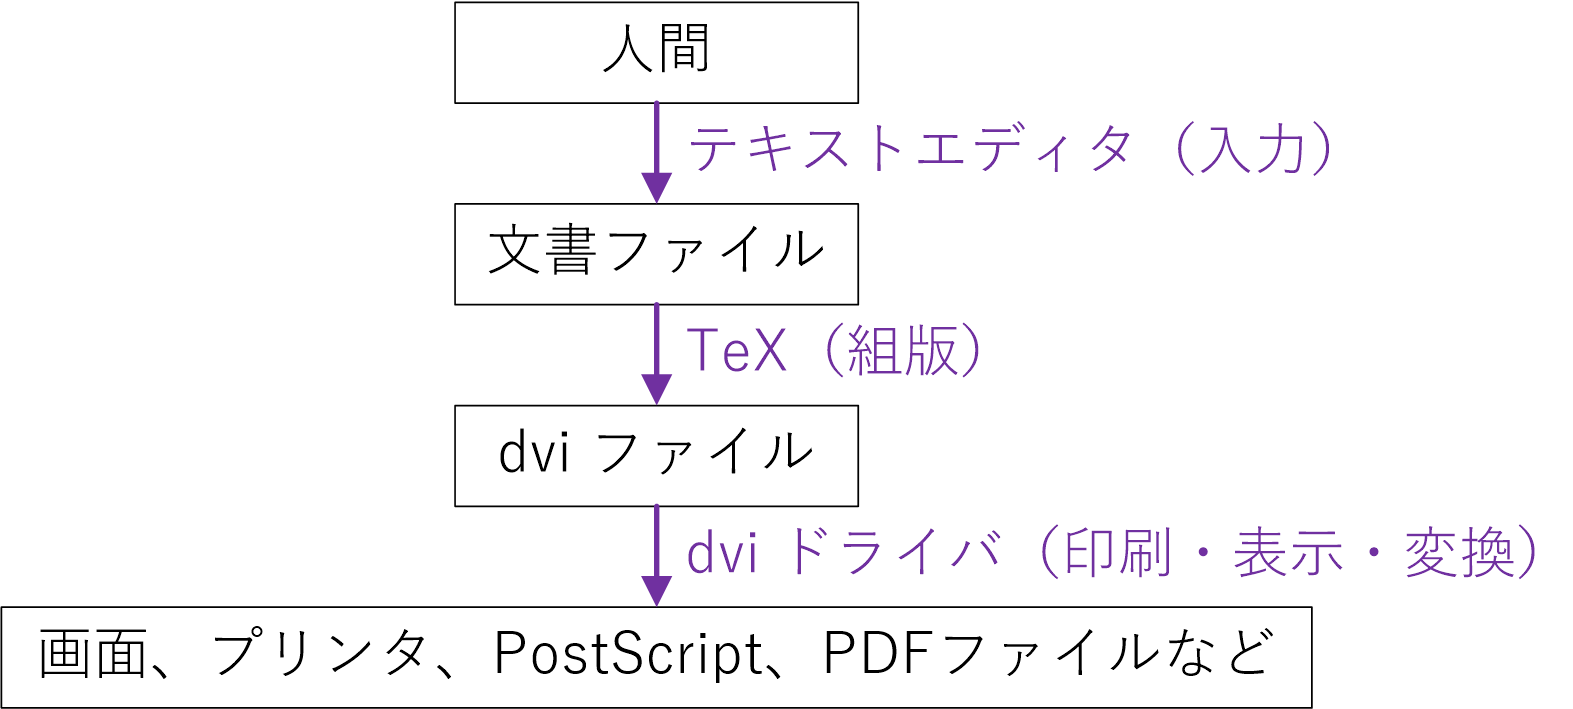
\includegraphics{./Part1/Fig/Fig01_01.PNG}}\caption{Part1で作成するスタンダードレイアウト}\label{Part1で作成するスタンダードレイアウト}\end{figure}\vspc{-3.00zw}
%%
%% 項:こんなことを学ぶ
%%----------------------------------------------------------------------------------------------------------%%
\subsection*{こんなことを学ぶ}
\vspc{-0.50zw}\begin{itemize}\setlength{\leftskip}{-1.00zw}%\setlength{\labelsep}{+1.00zw}
\item HTML5 の新要素
\item アウトライン
\end{itemize}\vspc{-1.50zw}
%%
%% 節:Part2:グリッドレイアウト
%%--------------------------------------------------------------------------------------------------------------------%%
\section{Part2:グリッドレイアウト}
ブラウザの横幅が変わるとブロックが自動で移動する可変グリッドレイアウトのサイトを作成する。
\vspc{-5.00pt}\begin{figure}[H]\centering\scalebox{0.37}{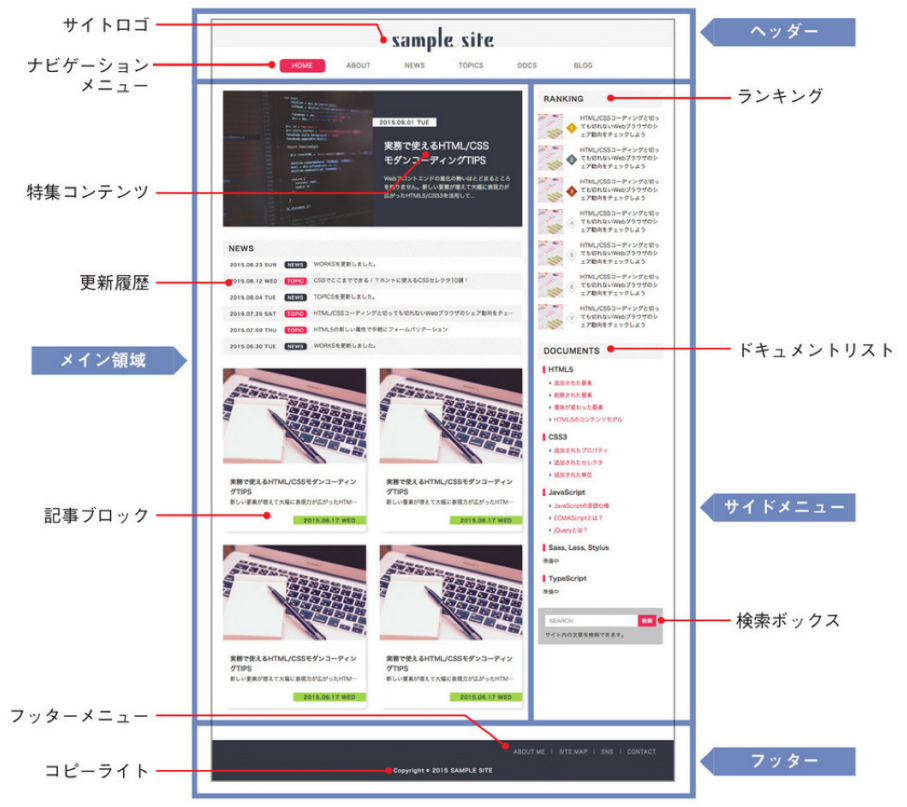
\includegraphics{./PART1/Fig/Fig01_02.PNG}}\caption{Part2で作成するグリッドレイアウト}\label{Part2で作成するグリッドレイアウト}\end{figure}\vspc{-3.00zw}
%%
%% 項:こんなことを学ぶ
%%----------------------------------------------------------------------------------------------------------%%
\subsection*{こんなことを学ぶ}
\vspc{-0.50zw}\begin{itemize}\setlength{\leftskip}{-1.00zw}%\setlength{\labelsep}{+1.00zw}
\item 可変グリッドレイアウトライブラリ
\item CSS アニメーション
\end{itemize}\vspc{-1.50zw}
%%
%% 節:Part3:グリッドレイアウト
%%--------------------------------------------------------------------------------------------------------------------%%
\section{Part3:シングルページレイアウト}
PC とスマートフォン両方に対応したシングルページレイアウトを作成する。
\vspc{-5.00pt}\begin{figure}[H]\centering\scalebox{0.45}{\includegraphics{./PART1/Fig/Fig01_03.PNG}}\caption{Part3で作成するシングルページレイアウト}\label{Part3で作成するシングルページレイアウト}\end{figure}\vspc{-3.00zw}
%%
%% 項:こんなことを学ぶ
%%----------------------------------------------------------------------------------------------------------%%
\subsection*{こんなことを学ぶ}
\vspc{-0.50zw}\begin{itemize}\setlength{\leftskip}{-1.00zw}%\setlength{\labelsep}{+1.00zw}
\item レスポンシブル Web デザイン
\item Web フォント
\end{itemize}\vspc{-1.50zw}
%%
%% 節:対応ブラウザ
%%--------------------------------------------------------------------------------------------------------------------%%
\section{対応ブラウザ}
本稿で作成するサイトの対応ブラウザは以下の通りである。
\vspc{-0.50zw}\begin{itemize}\setlength{\leftskip}{-1.00zw}%\setlength{\labelsep}{+1.00zw}
\item Internet Explorer 9 以上
\item Google Chrome
\item FireFox
\item Safari
\item シングルページレイアウトでのみ Mobile Safari、Chome to Mobile、Android Browser(Android 4.1 以降)
\end{itemize}\vspc{-0.50zw}
Internet Explore 8(以下、IE8 と記す)は 2016 年 1 月 12 日に Microsoft のサポート対象から外れ、セキュリティの更新やテクニカルサポートが提供されなくなったため、IE8 やそれ以下のレガシーブラウザは今後ますます使われなくなっていくことは明らかである。
そのため、本稿ではそれらのブラウザを対象ブラウザから除外している。\\

HTML5 に対応していないレガシーブラウザを除外することによって、コーディングに使える要素や機能がぐっと多くなるとともに、レガシーブラウザでの表示をフォローするための工夫も不要になるため、軽量で効率的なコーディングを行うことが可能となる。
これまでは比較的モダンとされていたようなコーディングが、IE8 のサポート終了以降も、もはやモダンではなくスタンダードとなっていくだろう。\\
%%
%% 節:コーディングの進め方
%%--------------------------------------------------------------------------------------------------------------------%%
\section{コーディングの進め方}
%%
%% 項:コーディングの前知識
%%----------------------------------------------------------------------------------------------------------%%
\subsection{コーディングの前知識}
本稿の解説で使用する HTML と CSS の各部の名称については以下の通りである。
\vspc{-0.50zw}\begin{longtable}{cl}
  \caption[]{HTML/CSSの各部名称\label{HTML/CSSの各部名称}}                                                                                                                \\[-1.30zw]\toprule
  \textgt{HTML} & \texttt{<\textcolor{orange}{要素名} \textcolor{blue}{属性}=}\verb|"|\texttt{\textcolor{red}{値}}\verb|"|\texttt{>テキスト</\textcolor{orange}{要素名}>} \\
  \textgt{CSS}  & \texttt{\textcolor{orange}{セレクタ} \{\,\textcolor{blue}{プロパティ}\hspc{+0.40pt}:\hspc{+1.00pt}\textcolor{red}{値}{;}\,\}}                           \\ \bottomrule
\end{longtable}\vspc{-0.90zw}
以下の CSS の基本的なセレクタについては、本稿の中では解説を省くことにする。
\vspc{-0.50zw}\begin{longtable}{ll}
  \caption[]{CSSの基本的なセレクタ\label{CSSの基本的なセレクタ}} \\[-1.30zw]\toprule
  \texttt{p}                       & 要素型                      \\ \midrule
  \texttt{{.}sample}\hspc{+4.00zw} & クラス\hspc{+3.00zw}        \\ \midrule
  \texttt{\#sample}                & id                          \\ \bottomrule
\end{longtable}\vspc{-0.90zw}
また、解説の中で、ある要素を示したい場合には CSS のセレクタと同様の表現を使用する。
%%
%% 項:コーディングする上でのポイント
%%----------------------------------------------------------------------------------------------------------%%
\subsection{コーディングする上でのポイント}
CSS コーディングの際に意識すると保守性が高まるポイントを紹介する。
本稿で扱うサンプルサイトも以下のポイントを踏まえて制作されている。
\vspc{-0.50zw}\begin{itemize}\setlength{\leftskip}{-1.00zw}%\setlength{\labelsep}{+1.00zw}
\item[\textcolor{red}{・}] \textcolor{red}{要素名にスタイルを指定しない} \\
  一度コーディングが終わっても、後から部分的な仕様の変更や対象ブラウザの変化などによって HTML のマークアップが変更される場合がある。
  そのような場合に要素名に対してスタイルを指定していると、HTML の編集と同時にセレクタを変更するために CSS ファイルも修正しなくてはならなくなる。
  但し、a要素、input要素、textarea要素など「その要素でないと機能が成り立たない」場合は要素の種類が変わる可能性が低いため、要素名に直接スタイルを指定するデメリットは小さくなる。
\item[\textcolor{red}{・}] \textcolor{red}{CSS のセレクタには ID ではなくクラスを使用する} \\
  CSS のセレクタにはクラスの他に ID も使用できるが、ID を避けた方がよい理由が 3 つある。\enlargethispage{0.50zw}
  \vspc{-0.00zw}\begin{itemize}\setlength{\leftskip}{-1.00zw}%\setlength{\labelsep}{+1.00zw}
  \item[\ajMaru{1}] \textbf{スタイルの使い回しができない} \\
    ID はクラスと異なり、同じページの中では 1 つの ID を複数回使えないという決まりがある。
    その為、ID にスタイルを指定してしまうと、そのスタイルは 1 つのページの中で一度までしか使用できなくなってしまう。
    最初のデザインではそれで問題なくても、後々の改善で同じデザインの要素を増やす必要が出てきた場合に問題となる。
  \item[\ajMaru{2}] \textbf{スタイルの上書きが難しい} \\
    CSS には詳細度という概念がある。
    詳細度とは、スタイルが適用される優先順位を決める仕組みである。詳しくは後述するが、ID はクラスよりも詳細度が高いので、ID で指定したスタイルは後からクラスで指定したスタイルで上書きすることができない。
  \item[\ajMaru{3}] \textbf{HTML や JavaScript と影響範囲を分離する} \\
    CSS セレクタはスタイルを指定したい要素を CSS から特定するためのものだが、要素の特定が必要な場合は CSS 以外でも発生する。
    HTML でページ内の特定の場所を指定してリンクする場合には ID を用いるし、JavaScript の処理で特定の 1 の要素を取得したい場合にも ID を使用すると効率がよい。
    前述した ID のルールに従い、同じ ID の要素が複数存在しないことを前提にできるので、絞り込みや重複確認をせずピンポイントで 1 つの要素を特定できるからである。
    そこで、ID は HTML、JavaScript からの特定に使用し、CSS セレクタは使用しないというようなルール付けをすると、影響範囲を分離できるので管理がし易くなる。
  \end{itemize}\vspc{-0.50zw}

\end{itemize}\vspc{-0.50zw}
%%
%% 項:リセット CSS について
%%----------------------------------------------------------------------------------------------------------%%
\subsection{リセット CSS について}
本稿で扱うサンプルサイトでは、解説の中で記述していく style.css の前に「リセットCSS」と呼ばれる CSS ファイルを読み込んでいる。\\

Web サイトを閲覧するブラウザは、それぞれ「ユーザエージェントスタイルシート(UAスタイルシート)」と呼ばれるスタイルシートを持っている。
ここには「h1要素は大きめの文字で太字」「p要素のまわりには間隔をあける」「ul要素にはリストマークを付ける」など、デフォルトで適用されるスタイルが記述されている。
そのおかげで、CSS が 1 行も書かれていない HTML 文書もある程度読み易く表示することができる。\\

便利な UA スタイルシートだが、次に挙げるような問題もある。
\vspc{-0.50zw}\begin{itemize}\setlength{\leftskip}{-1.00zw}%\setlength{\labelsep}{+1.00zw}
\item ブラウザごとに UA スタイルシートがあるため、適用される値のズレによって同じ HTML でもブラウザ間で表示が異なってしまう。
\item これから自分で記述するスタイルシートと UA スタイルシートの間に食い違いが存在すると、UA スタイルシートの不要なスタイルをわざわざ打ち消さなければならない。
\end{itemize}\vspc{-0.50zw}
これらの問題を解決してくれるのがリセット CSS である。
リセット CSS は各ブラウザの UA スタイルシートを一部リセットするための CSS で、この CSS を読み込むことで UA スタイルシートによる装飾がある程度まで打ち消され、ブラウザ間の差異をなくすことができる。\\

もう 1 つ似たものとして normalize.css という CSS もある。
これもブラウザ間での表示の差異をなくすという目的は reset.css と同じだが「リセット(初期化)」ではなく「ノーマライズ(統一する)」という名前の通り、UA スタイルシートの装飾を極力活かしながらブラウザ間の差異のみを埋めていくという点が異なる。\\

UA スタイルシートを活かせそうなサイトデザインであれば、こちらの CSS を読み込んだ方がコーディングの効率がよくなる場合がある。
本稿では、Part1 と Part2 では reset.css を、Part3 では normalize.css を利用している。

%%
%% 章:ベースのコーディング
%%------------------------------------------------------------------------------------------------------------------------------%%
\chapter{ベースのコーディング}
それぞれの箇所のコーディングに入る前に、サイト全体に影響する部分のコーディングを行う。
%%
%% 節:ファイル構成
%%--------------------------------------------------------------------------------------------------------------------%%
\section{ファイル構成}
\begin{wrapfigure}{r}{19.00zw}
  \vspace*{-\intextsep}
  \includegraphics[width=19.00zw]{./PART2/Fig/Fig01_03.PNG}
\end{wrapfigure}
今回制作するスタンダードレイアウトサイトのファイル構成を確認しておく。
ベースになるファイルは、翔泳社のダウンロードサイト\footnote{http://www.shoeisha.co.jp/book/download/9784798141572}で配布されている。
ファイルをダウンロードしたら css/reset.css と image/ 以下のファイルはダウンロードしたファイルをそのまま利用する。\\

メインとなる index.html と css/style.css をこれから記述していく。
%%
%% 節:要素とサイズの確認
%%--------------------------------------------------------------------------------------------------------------------%%
\section{要素とサイズの確認}

%%
%% 章:基本的な操作
%%------------------------------------------------------------------------------------------------------------------------------%%
\chapter{基本的な操作}
%%
%% 節:コマンド
%%--------------------------------------------------------------------------------------------------------------------%%
\section{コマンド}
Emacs はエディタなので文字入力ができるのは当然だが、文字を入力するだけなら単機能なエディタと同じであると言える。
Emacs が多くの開発者に愛されているのは、様々なことが行える優秀なコマンドが多く用意されているからである。
%%
%% 項:入力して実行する
%%----------------------------------------------------------------------------------------------------------%%
\subsection{入力して実行する}
コマンドを実行する方法は 2 通り存在する。\\

その 1 つがコマンド名を入力して実行する方法である。
Emacs 上で \raise0.3ex\hbox{\ovalbox{\footnotesize{\texttt{Alt\vphantom{x}}}}}+\raise0.3ex\hbox{\ovalbox{\footnotesize{\texttt{x\vphantom{l}}}}} を押すとミニバッファにフォーカスが移動し、コマンド入力待ちの状態となる。
この状態で、例えば \texttt{about} と入力して \raise0.3ex\hbox{\ovalbox{\footnotesize{\texttt{Tab\vphantom{T}}}}} を押してみる。
\raise0.3ex\hbox{\ovalbox{\footnotesize{\texttt{Tab\vphantom{T}}}}} はミニバッファで入力を補完してくれる非常に便利なキーである。
about から始まるコマンドは about-emacs のみなので about-emacs が補完されたはずである。
この状態で \raise0.3ex\hbox{\ovalbox{\footnotesize{\texttt{Enter\vphantom{E}}}}} キーを押すと、環境にインストールされている Emacs のバージョン情報が表示されるバッファが開く。\\

続いて、同じく \raise0.3ex\hbox{\ovalbox{\footnotesize{\texttt{Alt\vphantom{x}}}}}+\raise0.3ex\hbox{\ovalbox{\footnotesize{\texttt{x\vphantom{l}}}}} を押してコマンド入力待ちの状態にし、help-with-tutorial-spec-language と入力してみる。
今度はウィンドウが分割され、ミニバッファには Language: と表示されるはずである。
これは、更なる入力を求めている状態であり、japa と入力して \raise0.3ex\hbox{\ovalbox{\footnotesize{\texttt{Tab\vphantom{T}}}}} キーを押す。
Japanese が補完されるので \raise0.3ex\hbox{\ovalbox{\footnotesize{\texttt{Enter\vphantom{E}}}}} を押すと、Emacs チュートリアルの日本語版が開く。
このチュートリアルは、読み進めながら指示通りに操作することで Emacs の一連の操作をマスターすることができるようになっている。
%%
%% 項:キーバインドから実行する
%%----------------------------------------------------------------------------------------------------------%%
\subsection{キーバインドから実行する}
もう 1 つのコマンド実行方法はキーバインドから実行する方法である。
キーバインドとは一般的にキーボードショートカットと呼ばれるもので、修飾キーと文字キーを組み合わせた操作のことである。\\

Emacs には様々なキーバインドが用意されている。
このキーバインドを覚えることで、魔法のように速く編集を行うことができるようになる。\\

何か文字のある行の途中で \raise0.3ex\hbox{\ovalbox{\footnotesize{\texttt{Ctrl\vphantom{C}}}}}+\raise0.3ex\hbox{\ovalbox{\footnotesize{\texttt{a\vphantom{C}}}}} を押してみる。
すると、カーソルが行頭に移動する。
続けて \raise0.3ex\hbox{\ovalbox{\footnotesize{\texttt{Ctrl\vphantom{C}}}}}+\raise0.3ex\hbox{\ovalbox{\footnotesize{\texttt{e\vphantom{C}}}}} を押すと、今度はカーソルが行末に移動する。
これは、それぞれのキーバインドに beginning-of-line と move-end-line というコマンドが割り当てられ実行されているのである。\\

Emacs のコマンドはプログラムの関数となっており、それがキーに割り当てられている。
キーバインドには自分で好きなコマンドを割り当てることも可能なので、全てのコマンドをキーバインドから実行することも可能である。
%%
%% 款:コマンドの表記方法
%%------------------------------------------------------------------------------------------------%%
\subsubsection{コマンドの表記方法}
本稿でコマンドを表記する場合は次のように表記する。
\vspc{-0.50zw}\begin{itemize}\setlength{\leftskip}{-1.00zw}%\setlength{\labelsep}{+1.00zw}
\item[] \texttt{\textgt{M-x コマンド名}}
\end{itemize}\vspc{-0.50zw}
\texttt{M-x} は \raise0.3ex\hbox{\ovalbox{\footnotesize{\texttt{Alt\vphantom{x}}}}}+\raise0.3ex\hbox{\ovalbox{\footnotesize{\texttt{x\vphantom{l}}}}} と同じ意味で、この後「キーバインドの表記方法」で詳しく解説する。
尚、\texttt{M-x} は「メタエックス」もしくは「エムエックス」と読む。\\

コマンドに続けて更にミニバッファに入力を求められる場合は、
\vspc{-0.50zw}\begin{itemize}\setlength{\leftskip}{-1.00zw}%\setlength{\labelsep}{+1.00zw}
\item[] \texttt{\textgt{M-x コマンド名 RET 追加入力 RET}}
\end{itemize}\vspc{-0.50zw}
と表記する。
RET は \raise0.3ex\hbox{\ovalbox{\footnotesize{\texttt{Enter\vphantom{E}}}}} もしくは \raise0.3ex\hbox{\ovalbox{\footnotesize{\texttt{Ctrl\vphantom{C}}}}}+\raise0.3ex\hbox{\ovalbox{\footnotesize{\texttt{m\vphantom{C}}}}} を意味する。
%%
%% 款:キーバインドの表記方法
%%------------------------------------------------------------------------------------------------%%
\subsubsection{キーバインドの表記方法}
本稿でキーバインドを表記する場合は表\ref{キーバインド早わかり表}のように表記する。
\vspc{-0.50zw}\begin{longtable}{llllll}
  \caption[]{キーバインド早わかり表\label{キーバインド早わかり表}} \\[-1.30zw] \toprule
  \textgt{キーの種類} & \textgt{名前}  & \textgt{表記}           & \textgt{キーの種類} & \textgt{名前}  & \textgt{表記}               \\ \midrule\midrule
  装飾キー            & Control        & \texttt{C-}             & 特殊キー            & $\leftarrow$   & \texttt{<left>}             \\ \cmidrule{2-3}\cmidrule{5-6}
  {}                  & Meta           & \texttt{M-}             &                     & $\rightarrow$  & \texttt{<right>}            \\ \cmidrule{2-3}\cmidrule{5-6}
  {}                  & Shift          & \texttt{S-}             &                     & PageUp         & \texttt{<prior>}            \\ \cmidrule{2-3}\cmidrule{5-6}
  {}                  & Super          & \texttt{s-}             &                     & PageDown       & \texttt{<next>}             \\ \cmidrule{1-3}\cmidrule{5-6}
  文字・記号          & a,1,?,$\cdots$ & \texttt{a,1,?,$\cdots$} &                     & Home           & \texttt{<home>}             \\ \cmidrule{1-3}\cmidrule{5-6}
  特殊キー            & Tab            & \texttt{TAB}            &                     & End            & \texttt{<end>}              \\ \cmidrule{1-3}\cmidrule{5-6}
  {}                  & Space          & \texttt{SPC}            &                     & Backspace      & \texttt{<backspace>}        \\ \cmidrule{2-3}\cmidrule{5-6}
  {}                  & Escape         & \texttt{ESC}            &                     & Delete         & \texttt{<del>}              \\ \cmidrule{2-3}\cmidrule{5-6}
  {}                  & Return         & RET            &                     & Shift$+$TAB    & \texttt{<backtab>}          \\ \cmidrule{2-3}\cmidrule{5-6}
  {}                  & $\uparrow$     & \texttt{<up>}           &                     & F1,F2,$\cdots$ & \texttt{<f1>,<f2>,$\cdots$} \\ \cmidrule{2-3}\cmidrule{5-6}
  {}                  & $\downarrow$   & \texttt{<down>}         &                     &                &                             \\ \bottomrule
\end{longtable}\vspc{-1.50zw}
%%
%% 款:キーバインドの表記サンプル
%%------------------------------------------------------------------------------------------------%%
\subsubsection{キーバインドの表記サンプル}
キーバインドを説明する際、\texttt{C-n} や \texttt{M-x}、\texttt{C-x f} などの特殊な表記を用いるため、表\ref{キーバインドの表記}で説明しておく。
\vspc{-0.50zw}\begin{longtable}{ll}
  \caption[]{キーバインドの表記\label{キーバインドの表記}} \\[-1.30zw] \toprule
  \textgt{キー}      & \textgt{説明}                                                                                                                                                                                                                                                                                                              \\ \midrule\midrule
  \texttt{C-n}       & \raise0.2ex\hbox{\ovalbox{\footnotesize{\texttt{Ctrl\vphantom{C}}}}} を押しながら \raise0.2ex\hbox{\ovalbox{\footnotesize{\texttt{n\vphantom{C}}}}} を押す。                                                                                                                                                               \\ \midrule
  \texttt{M-f}       & \raise0.2ex\hbox{\ovalbox{\footnotesize{\texttt{Meta\vphantom{C}}}}} を押しながら \raise0.1ex\hbox{\ovalbox{\footnotesize{\texttt{f\vphantom{C}}}}} を押す。                                                                                                                                                               \\ \midrule
  \texttt{C-RET}     & \raise0.2ex\hbox{\ovalbox{\footnotesize{\texttt{Ctrl\vphantom{C}}}}} を押しながら \raise0.2ex\hbox{\ovalbox{\footnotesize{\texttt{Enter\vphantom{C}}}}} を押す。                                                                                                                                                           \\ \midrule
  \texttt{C-x k}     & \raise0.2ex\hbox{\ovalbox{\footnotesize{\texttt{Ctrl\vphantom{C}}}}} を押しながら \raise0.2ex\hbox{\ovalbox{\footnotesize{\texttt{x\vphantom{C}}}}} を押し、\raise0.2ex\hbox{\ovalbox{\footnotesize{\texttt{Ctrl\vphantom{C}}}}} を離してから \raise0.1ex\hbox{\ovalbox{\footnotesize{\texttt{k\vphantom{C}}}}} を押す。   \\ \midrule
  \texttt{C-x C-c}   & \raise0.2ex\hbox{\ovalbox{\footnotesize{\texttt{Ctrl\vphantom{C}}}}} を押しながら \raise0.2ex\hbox{\ovalbox{\footnotesize{\texttt{x\vphantom{C}}}}} を押し、そのまま \raise0.1ex\hbox{\ovalbox{\footnotesize{\texttt{c\vphantom{C}}}}} を押す。                                                                            \\ \midrule
  \texttt{C-M-S-v}   & \raise0.2ex\hbox{\ovalbox{\footnotesize{\texttt{Ctrl\vphantom{C}}}}} と \raise0.2ex\hbox{\ovalbox{\footnotesize{\texttt{Meta\vphantom{C}}}}} と \raise0.1ex\hbox{\ovalbox{\footnotesize{\texttt{Shift\vphantom{C}}}}}を押しながら \raise0.2ex\hbox{\ovalbox{\footnotesize{\texttt{v\vphantom{C}}}}} を押す。               \\ \midrule
  \texttt{C-/, C-\_} & \raise0.2ex\hbox{\ovalbox{\footnotesize{\texttt{Ctrl\vphantom{C}}}}} を押しながら \raise0.2ex\hbox{\ovalbox{\footnotesize{\texttt{/\vphantom{C}}}}}、もしくは \raise0.2ex\hbox{\ovalbox{\footnotesize{\texttt{Ctrl\vphantom{C}}}}}を押しながら \raise0.2ex\hbox{\ovalbox{\footnotesize{\texttt{\_\vphantom{C}}}}} を押す。 \\ \bottomrule
\end{longtable}\vspc{-0.70zw}
また、Emacs の解説では次のようにキーバインドの後にコマンド名を表記する場合がある。\enlargethispage{0.50zw}
\vspc{-0.50zw}\begin{itemize}\setlength{\leftskip}{-1.00zw}%\setlength{\labelsep}{+1.00zw}
\item[] \texttt{C-x C-f (find-file)}
\end{itemize}\vspc{-0.50zw}
これは \texttt{C-x C-f} と入力する他に \texttt{M-x find-file RET} としても利用可能である、という意味である。
本稿でも、キーバインドと同じ処理を実現するコマンドが存在する場合にはこの形で表記する。
%%
%% 款:プレフィックスキー(起点キー)
%%------------------------------------------------------------------------------------------------%%
\subsubsection{プレフィックスキー(起点キー)}
\texttt{C-x C-f} の \texttt{C-x} などは単体ではコマンドが実行されず、その後にキー入力を必要とするキーバインドである。
Emacs ではこのようなキーをプレフィックスキーと呼ぶ。
プレフィックスキーには、それぞれキーバインド設計のための指針が用意されているので、表\ref{プレフィックスキーの指針}で解説しておく。
\vspc{-0.50zw}\begin{longtable}{ll}
  \caption[]{プレフィックスキーの指針\label{プレフィックスキーの指針}} \\[-1.30zw] \toprule
  \textgt{キー} & \textgt{説明}                                                                   \\ \midrule\midrule
  \texttt{C-x}  & システムコマンドが利用する。                                                    \\ \midrule
  \texttt{C-c}  & ユーザがキーバインドを定義する。                                                \\ \midrule
  {}            & 拡張機能を作成する場合は \texttt{C-c} で始まるキーバインドは定義しない方がよい。\\ \midrule
  \texttt{M-g}  & 行移動に関するキーバインドが定義されている。                                    \\ \bottomrule
\end{longtable}\vspc{-1.50zw}
%%
%% 節:起動と終了
%%--------------------------------------------------------------------------------------------------------------------%%
\section{起動と終了}
起動と終了を説明しなければならないのは些か時代遅れな気がするが、Emacs は様々な OS や環境で利用できるように一般のアプリケーションより少々方法が多くなっているので、ここで解説しておく。
%%
%% 項:起動する
%%----------------------------------------------------------------------------------------------------------%%
\subsection{起動する}
最も簡単な Emacs の起動はアイコンをダブルクリックする方法である。
Mac では Emacs.app のアイコン、バイナリインストールした Windows では runemacs.exe のアイコンをダブルクリックして起動する。\\

ターミナルからは emacs、もしくは emacs-27.1 のようにバージョン番号を付けて起動する。
もし、X で起動する Emacs をターミナル内で起動したい場合は次のように -nw という引数を付加する。
\vspc{-0.50zw}\begin{itemize}\setlength{\leftskip}{-1.00zw}%\setlength{\labelsep}{+1.00zw}
\item[] \texttt{\textgt{\$ emacs -nw} もしくは \texttt{-{}-no-window-system}}
\end{itemize}\vspc{-0.50zw}
尚、Mac の Emacs.app もターミナル上で次のようにするとターミナル上で起動することができる。
\vspc{-0.50zw}\begin{itemize}\setlength{\leftskip}{-1.00zw}%\setlength{\labelsep}{+1.00zw}
\item[]\texttt{\textgt{\$ /Applications/Emacs.app/Contents/MacOS/Emacs -nw}}
\end{itemize}\vspc{-0.50zw}
Windows でもコマンドプロンプトもしくは PowerShell から bin\textyen{}emacs.exe に -nw 引数を付加して起動することで、プロンプト上で Emacs を利用可能である。
%%
%% 款:Emacs デーモンで起動を高速化する
%%------------------------------------------------------------------------------------------------%%
\subsubsection{Emacs デーモンで起動を高速化する}
Emacs は引数を付加して起動することで様々な状態で起動することが可能である。
主だった引数はターミナル上でで引数 -{}-help を付けて実行することで確認することができるが、覚えておきたいのが Emaacs デーモンである。\\

Emacs デーモンは Emacs 23 から導入された機能で、Emacs をデーモンと呼ばれるバックグランドで動作するプログラムとして起動しておくことで、瞬時に Emacs を起動させることができる仕組みである。\\

デーモンとして起動するには、Emacs に -{}-daemon という引数を付加して実行するだけである。
但し、Windows プラットフォームでは Emacs デーモンはサポートされていない。
\vspc{-0.50zw}\begin{itemize}\setlength{\leftskip}{-1.00zw}%\setlength{\labelsep}{+1.00zw}
\item[] \texttt{\$ emacs -{}-daemon}
\end{itemize}\vspc{-0.50zw}
デーモンとして起動しておいた Emacs を利用するには、emacsclient というコマンドを用いる。
\vspc{-0.50zw}\begin{itemize}\setlength{\leftskip}{-1.00zw}%\setlength{\labelsep}{+1.00zw}
\item[] \texttt{\$ emacsclient -c} もしくは \texttt{-{}-create-frame}
\end{itemize}\vspc{-0.50zw}
-c は主に X で Emacs を利用するために用いる。
ターミナル上で Emacs デーモンを利用する場合は次の通りである。
\vspc{-0.50zw}\begin{itemize}\setlength{\leftskip}{-1.00zw}%\setlength{\labelsep}{+1.00zw}
\item[] \texttt{\$ emacsclient -c} もしくは \texttt{-nw}
\end{itemize}\vspc{-0.50zw}
尚、Emacs デーモンは普通に終了してもバックグランドで起動し続けている。
本当に終了したい場合は、Emacs 上で \texttt{M-x kill-emacs} を実行するか、シェル上で次のコマンドを実行する。
\vspc{-0.50zw}\begin{itemize}\setlength{\leftskip}{-1.00zw}%\setlength{\labelsep}{+1.00zw}
\item[] \texttt{\$ emacsclient -e `(kill-emacs)`}
\end{itemize}\vspc{-0.50zw}
常に Emacs デーモンを利用したいのであれば、シェルにエイリアスを設定しておくとよい。\\

また、OS の起動スクリプトを利用して OS に起動と同時に自動的に Emacs デーモンを起動する方法が「Emacs Wiki: Emacs As  Daemon」\footnote{http://www.emacswiki.org/emacs/EmacsAsDaeom}に紹介されている。
%%
%% 款:デバックモードで起動する
%%------------------------------------------------------------------------------------------------%%
\subsubsection{デバックモードで起動する}
Emacs は第 4 章で解説する設定ファイル(init.el)を用意することで、起動時にユーザが記述した設定を読み込むようになる。
その際、設定に記述ミスがあると途中でエラーが発生し、それ以降の読み込みを中断する。
そのような場合、デバックモードで起動することでエラーの原因を調べることができる。\\

例えば、以下のような設定ファイルを読み込むようにしていたとする。
\vspc{+0.50zw}\begin{mdframed}[roundcorner=0.50zw,leftmargin=3.00zw,rightmargin=3.00zw,skipabove=0.40zw,skipbelow=0.40zw,innertopmargin=4.00pt,innerbottommargin=4.00pt,innerleftmargin=5.00pt,innerrightmargin=5.00pt,linecolor=gray!020,linewidth=0.50pt,backgroundcolor=gray!20]
\begin{verbatim}
;; cl-lib パッケージを読み込む。
(require `cl-lib)
;; スタートアップメッセージを非表示にする。
(setq inhibit-startup-screen t)
p(when window-system  % ← 行頭に不要な p が入っている
  ;; tool-bar を非表示にする。
  (tool-bar-mode 0)
  ;; scroll-bar を非表示にする。
  (scroll-bar-mode 0))
\end{verbatim}
\end{mdframed}\vspc{-0.70zw}
すると、Emacs は起動時に以下のようなエラーを出力する。
\vspc{+0.50zw}\begin{mdframed}[roundcorner=0.50zw,leftmargin=3.00zw,rightmargin=3.00zw,skipabove=0.40zw,skipbelow=0.40zw,innertopmargin=4.00pt,innerbottommargin=4.00pt,innerleftmargin=5.00pt,innerrightmargin=5.00pt,linecolor=gray!090,linewidth=0.50pt,backgroundcolor=gray!90]\color{gray!10}
\begin{verbatim}
Warning (initilaization): An error occured while loding `/Usrs/ユーザ名/.emacs.d/
init.el` :

Symbol's value as variable is boid: p

To ensure normal operation, you should investigate and remove the cause of the
error in your initialization file. Start Emacs with fg4the `--debag-init' option
to view a complete error backtrace.
\end{verbatim}
\end{mdframed}\vspc{-0.70zw}
この大まかな意味は「init.el ファイルを読み込み時にエラーが発生しました。p というシンボル変数は存在しません」である。
そして最後に「-{}-debag-init オプションを利用することで、完全なエラーのバックトレースを見ることができます」という説明が書かれている。
実際に -{}-debag-init を付加して起動してみると、Emacs 上で次のように表示される。
\vspc{-1.00zw}\begin{mdframed}[roundcorner=0.50zw,leftmargin=3.00zw,rightmargin=3.00zw,skipabove=0.40zw,skipbelow=0.40zw,innertopmargin=4.00pt,innerbottommargin=4.00pt,innerleftmargin=5.00pt,innerrightmargin=5.00pt,linecolor=gray!090,linewidth=0.50pt,backgroundcolor=gray!90]\color{gray!10}
\begin{verbatim}
Debugger entered--Lisp error: (void-variable p)
  eval-buffer(#<buffer *load> nil "/Users/ユーザ名/.emacs.d/init.el" nil t) ;
Readnig at buffer position 92
  load-with-code-conversion("/Users/ユーザ名/.emacs.d/init.el" "/Users/ユーザ名/
.emacs.d/init.el/" t t)
  load("/Users/ユーザ名/.emacs.d/init" t t)
  #[0 "H\205\266^Q \306=/203^Q^Q\307^H\310Q\202?^Q
  (中略)
  command-line()
  normal-top-level()
\end{verbatim}
\end{mdframed}\vspc{-0.70zw}
注目してほしいのは「Reading at buffer position 92」の部分である。
92 という数値は Emacs 内部の文字の場所(ポイントと呼ぶ)の数値である。\enlargethispage{1.00zw}
従って、この場所では init.el ファイルを開いて \texttt{M-x goto-char RET 92 RET} といコマンドを実行すると p という文字にカーソルが移動し、ここに p という文字が紛れ込んでいるのを発見することができる。
%%
%% 項:終了する
%%----------------------------------------------------------------------------------------------------------%%
\subsection{終了する}
Emacs を終了させるためには、通常 \texttt{C-c C-x} というキーバインドを利用する。
まだ保存されていないファイルが存在する場合は、ミニバッファに、
\vspc{-0.50zw}\begin{itemize}\setlength{\leftskip}{-1.00zw}%\setlength{\labelsep}{+1.00zw}
\item[] \verb|Save file /Users/ユーザ名/.emacs.d/init.el? (y, n, !, ., q, C-r, d or C-h)|
\end{itemize}\vspc{-0.50zw}
という質問が表示される。
この質問に対するそれぞれの指示は表\ref{未保存のファイルが存在する場合の対応}の通りである。
\vspc{-0.50zw}\begin{longtable}{ll}
  \caption[]{未保存のファイルが存在する場合の対応\label{未保存のファイルが存在する場合の対応}} \\[-1.30zw]\toprule
  \textgt{キー} & \textgt{説明}                                                                \\ \midrule\midrule
  \texttt{y}    & このファイルを保存する。                                                     \\ \midrule
  \texttt{n}    & このファイルを保存しない。                                                   \\ \midrule
  \texttt{!}    & 全てを保存する(未保存のファイルが複数存在する場合)。                       \\ \midrule
  \texttt{.}    & このファイルを保存して Emacs を終了する。                                    \\ \midrule
  \texttt{q}    & 全てのファイルを保存しない。                                                 \\ \midrule
  \texttt{C-r}  & ファイルを表示する(フレーム上に表示されていない場合)。                     \\ \midrule
  \texttt{d}    & 保存されているファイルと編集中のファイルの差分を表示する。                   \\ \midrule
  \texttt{C-h}  & 選択肢のヘルプを表示する。                                                   \\ \midrule
  \texttt{C-g}  & 操作をキャンセルする(何もしない)。                                         \\ \bottomrule
\end{longtable}\vspc{-0.50zw}
表\ref{未保存のファイルが存在する場合の対応}のキーを押すことで対応する操作が実行される。
未保存のファイルが複数存在する場合は全てのファイルに対して同じ質問が繰り返される。
保存を拒否したファイルが存在する場合、最後に次のように質問される。
\vspc{-0.50zw}\begin{itemize}\setlength{\leftskip}{-1.00zw}%\setlength{\labelsep}{+1.00zw}
\item[] \texttt{Modified buffers exist anyway? (yes or no)}
\end{itemize}\vspc{-0.50zw}
これは「変更がまだ残っていますが、本当に終了しますか?」という意味なので、\texttt{yes RET} とタイプすると変更を破棄して終了し、\texttt{no RET} で終了をキャンセルする。
\texttt{C-g} でもキャンセル可能である。
%%
%% 節:ファイル(バッファ)を開く、保存する
%%--------------------------------------------------------------------------------------------------------------------%%
\section{ファイル(バッファ)を開く、保存する}
Emacs はコマンドラインの時代から利用されているアプリケーションであるため、ファイルを開く、保存するなど非常に一般的な操作も通常はキーボードから操作する。
また、ここで解説するファイルの開き方はあくまで基本となる操作であり、第 6 章で解説する Helm という拡張機能を利用することで簡単にファイルを開くことが可能となる。
%%
%% 項:ファイル(バッファ)を開く
%%----------------------------------------------------------------------------------------------------------%%
\subsection{ファイル(バッファ)を開く:C-x C-f}
\texttt{C-x C-f (find-file)} というコマンドは、ファイルを開くための基本コマンドである。
カレントバッファのディレクトリを起点とし、ミニバッファにファイル名を入力する。
ミニバッファでは TAB による補完が利用できるため、慣れてくるとマウスでファイルを見つけてダブルクリックするよりも速くファイルを開くことができるようになる。\\

また、存在しないファイル名を入力するとバッファが作成され、保存時にディスクにファイルとして書き込まれる。
%%
%% 項:ファイル(バッファ)を保存する
%%----------------------------------------------------------------------------------------------------------%%
\subsection{ファイル(バッファ)を保存する:C-x C-s}
ファイルを開くという動作は、実際にはファイルを Emacs のバッファに読み込むという操作のことである。
従って、編集したバッファは保存するまでは実際のファイルに反映されない。
バッファを保存するには \texttt{C-x C-s (save-buffer)} というキーバインドを用いる。\\

尚、標準の設定では一番初めにファイルを保存する際、ファイルを開いた時の状態をバックアップファイル(後述)として保存する。
この機能を利用することで、何度保存しても最初に開いた時の状態に復元することができる。
%%
%% 項:全てのファイル(バッファ)を保存する
%%----------------------------------------------------------------------------------------------------------%%
\subsection{全てのファイル(バッファ)を保存する:C-x s}
\texttt{C-x s (save-some-buffers)} というコマンドも用意されている。
こちらは「Emacs の終了」で解説したものと同じで、Emacs 上で開いている全てのファイルに対して保存するか否かそれぞれ確認する。
%%
%% 項:バックアップファイル
%%----------------------------------------------------------------------------------------------------------%%
\subsection{バックアップファイル}
Emacs が作成するバックアップファイルは、ファイル名の末尾に \textasciitilde(チルダ)を付けた名前となっている。
例えば「init.el」というファイルであれば「init.el\textasciitilde」というファイルがバックアップファイルである。
%%
%% 款:オートセーブファイル
%%------------------------------------------------------------------------------------------------%%
\subsubsection{オートセーブファイル}
前述のバックアップファイルは Emacs が終了しても残り続けるが、これ以外にも Emacs には編集中のファイルのバックアップを随時作成するオートセーブという仕組みが用意されている。
これはアイドルタイム(Emacs を操作していない時間)を利用してファイル名の前と後ろに \# マークが付いたオートセーブファイルを自動的に作成してくれる。
尚、このオートセーブファイルはバッファをファイルに保存すると自動的に削除される。
このオートセーブに関する詳しい設定については第 5 章で解説する。
%%
%% 項:別名で保存する
%%----------------------------------------------------------------------------------------------------------%%
\subsection{別名で保存する:C-x C-w}
ファイルを別名で保存するには \texttt{C-x C-w (write-file)} というキーバインドを用いる。
コマンドを入力すると \texttt{C-x C-f (find-file)} と同じようにファイル名(パスも含めて)を聞かれるので、入力して RET とすると別名で保存される。
%%
%% 項:バッファに別ファイルを挿入する
%%----------------------------------------------------------------------------------------------------------%%
\subsection{バッファに別ファイルを挿入する:C-x i}
現在開いているバッファに別のファイルを挿入することも可能である。
\texttt{C-x i (insert-file)} を実行すると、ミニバッファで「Insert file:」とファイル名を聞かれるので、ファイルを開く時と同様にファイル名を入力するだけで簡単にファイルを挿入することができる。
また、\texttt{M-x insert-buffer} でバッファを挿入することも可能である。
すなわち、既に Emacs で開いているファイルまたは Emacs が自動生成するバッファの内容を挿入することができる。
%%
%% 項:文字コード・改行コードを変換する
%%----------------------------------------------------------------------------------------------------------%%
\subsection{文字コード・改行コードを変換する:C-x RET f}
最近は意識する必要が少なくなったとはいえ、テキストファイルを扱う上で忘れてならないのが文字コードと改行コードである。\\

Emacs はエディタの中でも最も多くの文字コードを扱うことができるエディタの 1 つである。
基本的には自動判別して適切な文字コードでファイルを開いてくれる。
尚、Emacs でファイルを作成した際の標準文字コードは Unicode(UTF-8)、改行コードは UNIX(LF)となっている。\\

現在編集中のバッファの文字コードを変更したい場合は、\texttt{C-x RET f (set-buffer-file-coding-system)} というキーバインドを用いる。
実行するとミニバッファで「Coding system for saving file (default nil):」と問われるので、変更したい文字コードの名前(コーディングシステム名)を入力すると文字コードが変更される。
例えば、sjis-dos とすると Shift-JIS で CR+LF、sjis であれば Shift-JIS で改行コードは変更しないという意味となる。\\

指定可能な文字コードを表\ref{文字コード}、改行コードを表\ref{改行コード}に示す。
\vspc{-0.50zw}\begin{longtable}{lll}
  \caption[]{文字コード\label{文字コード}} \\[-1.30zw] \toprule
  \textgt{モードライン表記} & \textgt{文字コード名} & \textgt{Emacs 上の呼称}                                 \\ \midrule\midrule
  \texttt{U}                & Unicode               & utf-8、utf-16、utf-7 など                               \\ \midrule
  \texttt{S}                & Shift\_JIS            & sjis(shift\_jis)                                      \\ \midrule
  \texttt{J}                & JIS コード            & iso-2022-jp など                                        \\ \midrule
  \texttt{E}                & 日本語 EUC            & euc-jp、euc-jis-2004 など                               \\ \midrule
  \texttt{1}                & Lattin-1              & latin-1(iso$-$8859$-$1)                               \\ \midrule
  \texttt{M}                & emacs-mule            & emacs-mule                                              \\ \bottomrule
\end{longtable}\vspc{-1.50zw}
\vspc{-0.50zw}\begin{longtable}{llll}
  \caption[]{改行コード\label{改行コード}} \\[-1.30zw] \toprule
  \textgt{モードライン表記} & \textgt{改行コード名} & \textgt{Emacs 上の呼称} & 説明                          \\ \midrule\midrule
  \texttt{:}                & LF                    & unix                    & UNIX 系 OS で主に利用される。 \\ \midrule
  \texttt{(DOS)}            & CR+LF                 & dos                     & Windows で主に利用される。    \\ \midrule
  \texttt{(Mac)}            & CR                    & mac                     & Mac OS 9 まで利用されていた。 \\ \bottomrule
\end{longtable}\vspc{-1.00zw}
文字コードの選択でも TAB による補完と候補一覧を利用することができる。
%%
%% 項:文字コード・改行コードを変換して開き直す
%%----------------------------------------------------------------------------------------------------------%%
\subsection{文字コード・改行コードを変換して開き直す:C-x RET r}
次は、途中変更ではなく文字コードを指定して開き直す方法である。
\texttt{C-x RET r (revert-buffer-with-coding-sys\\tem)} というキーバインドで、前述と同様に文字コードを問われるので入力するとファイル名を指定した文字コードで開き直してくれる。
%%
%% 項:バッファを切り替える
%%----------------------------------------------------------------------------------------------------------%%
\subsection{バッファを切り替える:C-x b}
今までも何度か登場したが、Emacs ではファイルを開くとバッファを作成し、消去しない限り Emacs 上に保持し続ける。
これはブラウザで言うところのタブのようなもので、タブを切り替えるようにバッファを切り替えることで複数のファイルを 1 つの Emacs で編集することができる。\\

バッファを切り替えるには \texttt{C-x b (switch-to-buffer)} というキーバインドを用いる。
するとミニバッファでバッファ名を問われるので入力して RET を押す。
この時、勿論 TAB による補完が利用可能である。
いちいちバッファ名を入力するのが煩わしい場合は、\texttt{C-x <right> (next-buffer)}、\texttt{C-x <left> (previous-buffer)} というキーバインドを利用するとよいだろう。
これは Emacs 内で管理しているバッファリストに従って、バッファを順番に切り替えてくれる。
バッファリストの確認は \texttt{C-x C-b (list-buffers)} というキーバインドで可能である。
%%
%% 項:バッファを消去する
%%----------------------------------------------------------------------------------------------------------%%
\subsection{バッファを消去する:C-x k}
バッファを消去するには \texttt{C-x k (kill-buffer)} というキーバインドを用いる。
すると消去するバッファを問われるので、そのまま RET するとカレントバッファが消去される。\\

もし、そのバッファがまだ保存されていない場合は「buffer バッファ名 modified; kill anyway? (yes or no)」と問われるので、yes と入力するとバッファを保存せずに消去、すなわち編集を破棄する。
no または \texttt{C-g} でバッファの消去をキャンセルする。
%%
%% 節:カーソル移動
%%--------------------------------------------------------------------------------------------------------------------%%
\section{カーソル移動}
次はカーソル移動である。
第 1 章でも述べたが、Emacs を使うメリットとしてキーボードで思い通りのカーソル移動ができるという点が挙げられる。
その優れた操作性を身に付けることで、とても快適な編集を実現してくれる。
%%
%% 項:キーバインド一覧
%%----------------------------------------------------------------------------------------------------------%%
\subsection{キーバインド一覧}
カーソル移動については、Emacs チュートリアルで一通り学ぶことができるが、改めて主要なキーバインド一覧を表\ref{カーソル移動系の主要キーバインド}にまとめておく。
\vspc{-0.50zw}\begin{longtable}{lll}
  \caption[]{カーソル移動系の主要キーバインド\label{カーソル移動系の主要キーバインド}}  \\[-1.30zw] \toprule
  \textgt{キー}    & \textgt{コマンド名}               & \textgt{説明}                                                      \\ \midrule\midrule
  \texttt{C-l}     & \texttt{recenter-top-bottom}      & カーソル位置を起点にウィンドウの表示をリフレッシュする。           \\ \midrule
  \texttt{C-p}     & \texttt{backward-line}            & 1 つ上の行に移動する。                                             \\ \midrule
  \texttt{C-n}     & \texttt{next-line}                & 1 つ下の行に移動する。                                             \\ \midrule
  \texttt{C-f}     & \texttt{previous-line}            & 1 文字前に移動する。                                               \\ \midrule
  \texttt{C-b}     & \texttt{previous-line}            & 1 文字後に移動する。                                               \\ \midrule
  \texttt{C-a}     & \texttt{move-beginning-of-line}   & 行頭に移動する。                                                   \\ \midrule
  \texttt{C-e}     & \texttt{move-end-of-line}         & 行末に移動する。                                                   \\ \midrule
  \texttt{C-v}     & \texttt{scroll-up-command}        & 1 画面下にスクロールする。                                         \\ \midrule
  \texttt{M-v}     & \texttt{scroll-down-command}      & 1 画面上にスクロールする。                                         \\ \midrule
  \texttt{C-M-v}   & \texttt{scroll-other-window}      & ウィンドウ分割時に他のウィンドウに対して \texttt{C-v} を実行する。 \\ \midrule
  \texttt{C-M-S-v} & \texttt{scroll-other-window-down} & ウィンドウ分割時に他のウィンドウに対して \texttt{M-v} を実行する。 \\ \midrule
  \texttt{M-<}     & \texttt{beginning-of-buffer}      & バッファの先頭へ移動する。                                         \\ \midrule
  \texttt{M->}     & \texttt{end-of-buffer}            & バッファの終端へ移動する。                                         \\ \midrule
  \texttt{M-g g}   & \texttt{goto-line}                & ミニバッファで入力した行番号へ移動する。                           \\ \bottomrule
\end{longtable}\vspc{-1.50zw}
%%
%% 節:文字の入力や文字列の操作
%%--------------------------------------------------------------------------------------------------------------------%%
\section{文字の入力や文字列の操作}
続いては入力に関する操作である。
通常の文字タイピングに関しては特筆すべき事はないが、コピーやカット、ペーストなどの入力補助については大いに有用である。
%%
%% 項:マークとリージョン
%%----------------------------------------------------------------------------------------------------------%%
\subsection{マークとリージョン:C-SPC}
コピーやカットを行う為には、まず範囲選択を行う。
この範囲選択はメモ帳などのエディタでは \raise0.2ex\hbox{\ovalbox{\footnotesize{\texttt{Shift\vphantom{$\uparrow$}}}}}+\raise0.3ex\hbox{\ovalbox{\footnotesize{ $\uparrow$ }}} \raise0.3ex\hbox{\ovalbox{\footnotesize{ $\downarrow$ }}} \raise0.3ex\hbox{\ovalbox{\footnotesize{$\leftarrow$\vphantom{$\uparrow$}}}} \raise0.3ex\hbox{\ovalbox{\footnotesize{$\rightarrow$}\vphantom{$\uparrow$}}} を用いるのが一般的だが、Emacs では一風変わった範囲選択方法が用意されている。
それがマークとリージョンという概念である。\\

マークは言葉の通りカーソル位置にマーキング(印付け)を行う操作である。
キーバインドは \texttt{C-SPC (mark-set-command)} もしくは \texttt{C-@} である。
マークしてからカーソル移動すると、マークから現在位置までが選択範囲となる。
これがリージョンである。
Emacs はリージョンを用いてコピーやカットなどの一般的な操作から整形、変換など高度な処理を行うことができる。
%%
%% 項:コピーとカット
%%----------------------------------------------------------------------------------------------------------%%
\subsection{コピーとカット:M-w、C-w}
リージョンを学んだ上で、コピーとカットの方法を解説する。
まずはコピーだが、リージョンによる範囲選択を行ってから \texttt{M-w (kill-ring-save)} というキーバインドを用いるとリージョンをコピーしてくれる。\\

コマンド名に kill-ring(キルリング)という言葉が入っているが、これは一般的にクリップボードと呼ばれるような機構で、消去(キル)したテキストを記録しておく場所となっている。\\

カットはコピーと同じくリージョンを作成してから \texttt{C-w (kill-region)} というキーバインドを用いる。
コマンド名は kill-region となっているが、このキルは消去という意味であり、キルされたテキストは全てキルリングに記録される。
尚、キルリングに記録しない文字の消去は削除(delete)と表現し、コマンド名も delete から始まるものが用いられる。
%%
%% 項:行を消去する
%%----------------------------------------------------------------------------------------------------------%%
\subsection{行を消去する:C-k}
少し特殊な操作として行の消去がある。
\texttt{C-k (kill-line)} はカーソル位置より右にあるテキストを行末まで(改行は含まない)を消去する。
消去なのでテキストはキルリングに記録される。
非常によく用いられる操作としては、行頭へ移動して行を消去する \texttt{C-a C-k} が挙げられる。\\

\texttt{C-k} はカーソルが改行に位置する場合、改行のみを消去する。
また、連続して \texttt{C-k} を用いて消去した内容は 1 回のペーストで貼り付けることができるようになっている。
%%
%% 項:ペーストする
%%----------------------------------------------------------------------------------------------------------%%
\subsection{ペーストする:C-y、C-y M-y}
コピーやカットなどで消去され、キルリングに記憶されたテキストは \texttt{C-y (yank)} を用いていつでもヤンク(ペースト)可能である。
このヤンクは直前に消去された内容を貼り付けるコマンドである。\\

以前にキルリングに記録した内容を遡ってヤンクするには、\texttt{C-y} に続けて \texttt{M-y (yank-pop)} を入力する。
\texttt{M-y} は直前のコマンドが \texttt{C-y} だった場合にのみ利用可能なコマンドで、キルリングの内容を遡ってヤンクする。
\texttt{M-y} を続けて入力することでキルリングを遡り続けるのだが、インタフェースとしては少々使いづらいものであるため、第 6 章で紹介する helm-show-kill-ring という拡張機能を利用する方がよいかもしれない。
%%
%% 項:コメントする、コメントを解除する
%%----------------------------------------------------------------------------------------------------------%%
\subsection{コメントする、コメントを解除する:M-;}
コメントとはコードや設定ファイルにおいて処理に含めない部分のことであり、読む人間のためのメモ書きやコード処理させないようにする(コメントアウトする)などに利用する。
Emacs には \texttt{M-; (comment-dwin)} という言語と状況によってコメントを挿入・解除してくれるコマンドが備わっている。
\vspc{-0.50zw}\begin{itemize}\setlength{\leftskip}{-1.00zw}%\setlength{\labelsep}{+1.00zw}
\item リージョン選択中に \texttt{M-;} するとコメントアウト、もしくはコメント解除する。
\item リージョン選択中に \texttt{C-u 数値 M-;} するとコメント文字列を数値分にする。
\item 何も書かれていない行(空行)で \texttt{M-;} した場合、コメント文字列を挿入する。
\item 何か書かれている行で \texttt{M-;} した場合、行末にコメント文字列を挿入する。
\item コメントが存在する行で \texttt{M-;} した場合、コメント本文までジャンプする。
\item コメント行で引数を与えて \texttt{M-;} した(例えば \texttt{C-u M-;})場合、コメント行であれば削除する。
\end{itemize}\vspc{-0.50zw}
編集中のファイルが特有のコメント開始文字を持たない場合はミニバッファで「No comment syntax is defined. Use:」と問われるので、例えば \# として RET すると \# をコメント開始記号として利用してくれる。
%%
%% 項:特殊文字を入力する
%%----------------------------------------------------------------------------------------------------------%%
\subsection{特殊文字を入力する:C-q}
テキストには、例えば改行文字やタブ文字など通常の文字とは異なる文字(制御文字など)が存在する。
これらを入力する方法を覚えておくと、思わぬところで役立つ可能性がある。
\texttt{C-q (quoted-insert)} は、次に入力したキーの制御文字を挿入してくれる。
例えば、リターンではなく改行文字そのものを挿入したい場合は \texttt{C-q C-j} を実行する。
同じくインデントではなくタブ文字を挿入したい場合は \texttt{C-q TAB} を実行し、\raise0.3ex\hbox{\ovalbox{\footnotesize{\texttt{Ctrl\vphantom{C}}}}}+\raise0.3ex\hbox{\ovalbox{\footnotesize{\texttt{c\vphantom{C}}}}} の制御文字を挿入したい場合は \texttt{C-q C-c} を実行する。
この \texttt{C-q} による特殊文字の入力を覚えておくと、例えば一括変換で改行を消去したり、カンマ(,)を改行に変換したりすることなどが簡単に行えるようになる。
%%
%% 項:アンドゥ
%%----------------------------------------------------------------------------------------------------------%%
\subsection{アンドゥ:C-/、C-\_、C-x u}
入力中に編集内容を 1 つ前の状態に戻したい場合はアンドゥを利用する。
\texttt{C-/ (undo)} を実行すると、直前の変更を元の状態に戻すことが可能である。\\

アンドゥとは逆の操作を実現するリドゥは Emacs 標準には用意されておらず、\texttt{C-g} を実行してからアンドゥを行うことでリドゥとの機能を実現する。
この操作に馴染めない場合は、第 6 章で紹介する拡張機能 undo-tree を導入するとよいだろう。\enlargethispage{1.00zw}
%%
%% 節:Emacs の正規表現
%%--------------------------------------------------------------------------------------------------------------------%%
\section{Emacs の正規表現}
Emacs では他のエディタ同様、検索や置換などに正規表現を利用することができる。
正規表現については本節ではあまり深く語らないが、Emacs の正規表現は文字列で記述するため、一般的な正規表現リテラルによる記述とは少々異なり注意が必要な部分が存在する。
%%
%% 項:特別な文字
%%----------------------------------------------------------------------------------------------------------%%
\subsection{特別な文字}
特別な文字とは一般的にメタキャラクタと呼ばれるもので、普通の文字とは異なり特殊な意味を持つ文字のことである。
表\ref{正規表現で使うことのできる特別な文字(メタキャラクタ)}にメタキャラクタを示す。
\vspc{-0.50zw}\begin{longtable}{lp{18zw}p{22zw}}
  \caption[]{正規表現で使うことのできる特別な文字(メタキャラクタ)\label{正規表現で使うことのできる特別な文字(メタキャラクタ)}} \\[-1.30zw] \toprule
  \textgt{文字}                                                         & \textgt{説明}                                                                  & \textgt{利用例}                                                                                                                \\ \midrule\midrule
  \texttt{.}                                                            & 改行以外の任意の文字に一致する。                                               & .macs(Emacs, imacs などに一致)                                                                                               \\ \midrule
  \textasteriskcentered{}                                               & 直前の正規表現を可能な限り反復する後置演算子。                                 & E\textasteriskcentered{}macs(macs, Emacs, EEEmacs などに一致)                                                                \\ \midrule
  \texttt{+}                                                            & 直前の正規表現に 1 回以上一致する。                                            & E+macs(Emacs, EEmacs, EEEmacs などに一致)                                                                                    \\ \midrule
  \texttt{?}                                                            & 直前の正規表現に 1 回以上一致するか、あるいは 1 回も一致しない。               & E?macs(macs, Emacs に一致)                                                                                                   \\ \midrule
  \texttt{\textbackslash\{n\}\textbackslash}                            & 直前の正規表現がn回の場合のみ一致する後置演算子。                             & E\textbackslash\{2\textbackslash\}macs(EEmacs に一致)                                                                        \\ \midrule
  \texttt{\textbackslash\{n, m\textbackslash\}}                         & 直前の正規表現がn回からm回まで一致する後置演算子。                           & E\textbackslash\{1, 3\textbackslash\}macs(Emacs, EEmacs, EEEmacs に一致)                                                     \\ \midrule
  \texttt{[\hphantom{.}\ldots\hphantom{\^{}}]}                          & この間にある文字集合に一致する。                                               & [Ee]macs(Emacs, emacs に一致)                                                                                                \\ \midrule
  \texttt{[\^{}\ldots\hphantom{\^{}}]}                                  & この間にある文字集合以外に一致する。                                           & [\^{}Ee]macs(Emacs, emacs 以外に一致)                                                                                        \\ \midrule
  \texttt{\^{}}                                                         & 行頭に一致する。                                                               & \^{}Emacs(行頭の Emacs に一致)                                                                                               \\ \midrule
  \texttt{\$}                                                           & 行末に一致する。                                                               & Emacs\$(行末の Emacs に一致)                                                                                                 \\ \midrule
  \texttt{\textbackslash}                                               & 特別な文字をクオート(エスケープ)する。\textbackslash{}.は文字{.}に一致する。 & \textbackslash{}.emacs(.emacs に一致)                                                                                        \\ \midrule
  \texttt{\textbackslash{}|}                                            & 両端の正規表現のどちらかに一致する。通常はグループ化と組合わせて使用する。     & a\textbackslash|{}b(a か b に一致する)                                                                                       \\ \midrule
  \texttt{\textbackslash(\hphantom{.}\ldots\hphantom{.}\textbackslash)} & グループ化。囲まれた正規表現を 1 つの文字のように扱う。                        & \textbackslash{}(Emacs\textbackslash{}|emacs\textbackslash)(Emacs か emacs に一致)                                           \\ \midrule
  \texttt{\textbackslash{}1,\textbackslash{}2,\ldots,\textbackslash{}9} & グループ化した文字を引用する。                                                 & \textbackslash(Emacs\textbackslash).\textasteriskcentered{}?\textbackslash{}1(Emacs から同じ行に登場する次の Emacs まで一致) \\ \bottomrule
\end{longtable}\vspc{-1.50zw}
%%
%% 節:検索と置換
%%----------------------------------------------------------------------------------------------------------%%
\section{検索と置換}
検索と置換はエディタの中心機能の 1 つである。
そもそも、検索は見つけるという操作以外にも移動したり思い出すなど様々な役割があり、OS を含む全てのアプリケーションにおいて検索を使いこなせるか否かで作業効率が大幅に変化する。
%%
%% 項:grep による検索
%%----------------------------------------------------------------------------------------------------------%%
\subsection{grep による検索}
grep とは UNIX 系 OS における検索の代名詞とも言えるコマンドであり、指定されたファイルの中から正規表現を用いて検索して一致する行を一覧表示してくれるものである。
Emacs には \texttt{M-x grep} というコマンドが用意されており、Emacs から直接 grep を実行することができる。
\texttt{M-x grep RET} と入力すると「Run grep (like this): grep -nH -e」という内容がミニバッファに表示される。
これはターミナルにおいて grep を実行する場合と同じ要領でコマンドを入力せよ、という要求である。
検索対象となるディレクトリはカレントディレクトリとなる。\\

例えば、emacs という単語を全てのファイルから検索したい場合、\verb'grep -nH -e "emacs" * RET' と入力する。
すると *grep* というバッファが開かれ、通常の grep と同様に一致した行が一覧表示される。\enlargethispage{0.50zw}
この一覧表からファイルを直接開くことが可能である。\\

通常の grep 以外にも対話式 grep コマンドである lgrep、再帰的に grep を行う rgrep というコマンドも用意されており、両方とも有用である。
%%
%% 項:インクリメンタル検索
%%----------------------------------------------------------------------------------------------------------%%
\subsection{インクリメンタル検索:C-s、C-r、C-M-s、C-M-r}
\texttt{C-s (isearch-forward)} は Emacs で非常によく利用されるキーバインドの 1 つである。
ミニバッファで「I-search:」と問われるので、文字を入力するとインクリメンタル検索が開始され、カレントバッファ上のカーソル以降にあるマッチ(一致)する文字の場所へカーソルがジャンプする。
尚、\texttt{C-r (isearch-backward)} は \texttt{C-s} とは逆にカーソル以前のマッチする文字へジャンプする。\\

\texttt{C-s} や \texttt{C-r} は検索している際に連続で入力すると、次にマッチする場所までカーソルが移動する。
これによって本文検索とカーソル移動を同時に実現することができる。\\

\texttt{C-M-s (isearch-forward-regexp)} は regexp という名前の付く通り isearch の正規表現版である。
%%
%% 項:対話置換、一括置換
%%----------------------------------------------------------------------------------------------------------%%
\subsection{対話置換、一括置換:M-\%、C-M-\%}
文字列の置換は正しく利用することで確実にテキストを置き換えてくれる。
Emacs には正規表現を利用するかどうか、置換時に確認するかどうかという異なる条件の置換コマンドが 4 つ用意されている。
尚、置換は全てカーソル以降に対してのみ行われるようになっており、カーソル以前は対象外となる。\\

\texttt{M-\%(query-replace)} は対話型の置換コマンドで、ミニバッファに検索する文字列、次に置換する文字列を入力することで置換が開始される。
検索にマッチした文字列を見つけるとカーソルが移動し「Query replacing 検索文字列 with 置換文字列: (?\hphantom{.}for help)」と問われる。
?\hphantom{.}を押すとヘルプが表示され、y で置換、n でスキップする。\\

\texttt{C-M-\%(query-replace-regexp)} は同じく対話型置換コマンドの正規表現利用版である。
\texttt{M-x replace-string} は対話無しで一括置換を行うコマンドであり、\texttt{M-x replace-string-regexp} は同じく一括置換の正規表現利用版である。
%%
%% 款:ナローイングを用いてバッファの一部のみを編集する
%%------------------------------------------------------------------------------------------------%%
\subsubsection{ナローイングを用いてバッファの一部のみを編集する}
ナローイング(narrowing)は普段あまり利用する機会のあるものではないが、意図しないキー操作によって実行される場合がある為、記憶に留めておいた方がよい仕組みである。\\

範囲を制限するという意味であるナローイングは、Emacs では編集可能範囲を制限するという意味で用いられる。
ある範囲だけを置換対象にしたい場合にも利用することができる。\\

リージョン選択時に \texttt{C-x n n (narrow-to-region)} というコマンドを実行すると、バッファからリージョンのみを残して他の部分が消え去る。\\

このコマンドは初心者にとって混乱の原因となる為、標準では利用できないようになっている。
そのため、初めて実行した際に本当に実行するかどうかを確認する問いが表示される。
\vspc{+0.05zw}\begin{mdframed}[roundcorner=0.50zw,leftmargin=3.00zw,rightmargin=3.00zw,skipabove=0.40zw,skipbelow=0.40zw,innertopmargin=4.00pt,innerbottommargin=4.00pt,innerleftmargin=5.00pt,innerrightmargin=5.00pt,linecolor=gray!090,linewidth=0.50pt,backgroundcolor=gray!90]\color{gray!10}
\begin{verbatim}
You have typed C-x n n, invoking disable command narrow-to-region.
It is disabled because new users often find it confusing.
Here's the first part of its description:

(中略)

You can now type
y   to try it and enable it (no question if you use it again).
n   to cancel--don't try the command, and it remains disabled.
SPC to try the command just this once, but leave it disabled.
!   to try it, and enable all disable commands for this session only.
\end{verbatim}
\end{mdframed}\vspc{-0.70zw}
そして、ミニバッファでは「Type y,n,!\hphantom{,}or\hphantom{,}SPC (the space bar):」という問いが表示され入力待ちとなる。
y を押すと narrow-to-regin が実行され、 2 度と同じ質問がされなくなる。
それぞの選択結果については表\ref{narrow-to-region の問いに対する選択結果}にまとめる。
\vspc{-0.60zw}\begin{longtable}{lp{42zw}}
  \caption[]{narrow-to-region の問いに対する選択結果\label{narrow-to-region の問いに対する選択結果}} \\[-1.30zw] \toprule
  \textgt{キー} & \textgt{説明}                                                                                                     \\ \midrule\midrule
  \texttt{y}    & narrow-to-region を実行。\texttt{(put `narrow-to-region `disable nil)} を設定ファイルに追加し、2 度と質問しない。 \\ \midrule
  \texttt{n}    & 実行をキャンセルする。次に実行する際は再度質問する。                                                              \\ \midrule
  \texttt{SPC}  & 今回は実行するが、次に実行する際は再度質問する。                                                                  \\ \midrule
  \texttt{!}    & 実行する。Emacs を終了するまで質問しない。                                                                        \\ \bottomrule
\end{longtable}\vspc{-0.60zw}
narrow-to-region を実行すると、モードラインに「Narrow」と表示され、リージョン以外が消えてしまった様な表示となるが、編集範囲を制限(隠した)だけである。
ナローイングを解除するワイドニングは \texttt{C-x n w (widen)} である。
ワイドニングを実行すると再び全体が表示される。
%%
%% 節:ウィンドウ操作
%%--------------------------------------------------------------------------------------------------------------------%%
\section{ウィンドウ操作}
Emacs を使っていると自動的にウィンドウ分割するコマンドが多々存在する為、本人が望まなくともウィンドウ操作を余儀なくされる。
最初の内は少々ややこしいかもしれないが、実際にウィンドウ操作で覚えなければならないものは最低でも以下の 3 つだけである。
%%
%% 項:ウィンドウを分割する
%%----------------------------------------------------------------------------------------------------------%%
\subsection{ウィンドウを分割する:C-x 2、C-x 3}
ウィンドウを分割するコマンドは 2 つのみである。
横に 2 分割する \texttt{C-x 2(split-window-vertically)} と、縦に分割する \texttt{C-x 3 (split-window-horizontally)} である。\\

vertically(垂直)と horizontally(水平)が、日本語の感覚としては逆であることが少々混乱を与えるが、横ではなく上下に分割するという意味合いから vertically と名付けられたのだろう。
覚え方としては、漢字の「二」のように分割するのが \texttt{C-x 2} であると捉えると記憶し易いかもしれない。
%%
%% 項:ウィンドウを移動する
%%----------------------------------------------------------------------------------------------------------%%
\subsection{ウィンドウを移動する:C-x o}
\texttt{C-x o (other-window)} は、ウィンドウが分割されている際に、カレントウィンドウを他のウィンドウへ移動するコマンドである。
%%
%% 項:分割したウィンドウを閉じる
%%----------------------------------------------------------------------------------------------------------%%
\subsection{分割したウィンドウを閉じる:C-x 1、C-x 0}
ウィンドウを閉じるコマンドは 2 つ用意されている。\\

1 つ目は \texttt{C-x 1 (delete-other-window)} で、実行するとカレントウィンドウ以外の全てのウィンドウを閉じる。\\

2 つ目は \texttt{C-x 0 (delete-window)} で、実行するとカレントウィンドウのみを閉じる。
状況に応じて使い分けると良いだろう。
因みに、ウィンドウを閉じてもバッファが削除されることはない。
%%
%% 節:ディレクトリ操作(Dired)
%%--------------------------------------------------------------------------------------------------------------------%%
\section{ディレクトリ操作(Dired)}
Emacs はテキストエディタだが、標準でディレクトリ操作が可能である。\\

それが Dired という機能である。
\texttt{C-x d (dired)} から \texttt{C-x C-f} と同じように開きたいディレクトリを指定して RET する。
すると、Dired というディレクトリエディタの為のバッファが開く。\\

Dired ではディレクトリやファイルのコピー、リネーム、作成、パーミッション変更など、標準的なファイラの機能は全て利用可能である。
基本操作を表\ref{Dired 上での代表的なコマンド一覧}にまとめる。
\vspc{-0.50zw}\begin{longtable}{llll}
  \caption[]{Dired 上での代表的なコマンド一覧\label{Dired 上での代表的なコマンド一覧}} \\[-1.30zw] \toprule
  \textgt{キー}        & \textgt{説明}                  & \textgt{キー} & \textgt{説明}                     \\ \midrule\midrule
  \texttt{n、SPC}      & 次の行へ移動する。             & \texttt{u}    & 現在行のマークを外す。            \\ \midrule
  \texttt{p}           & 前の行へ移動する。             & \texttt{*{}!} & マークを全て外す。                \\ \midrule
  \texttt{RET、f}      & 現在行のファイルを開く。       & \texttt{+}    & ディレクトリを作成する。          \\ \midrule
  \texttt{d}           & 削除候補としてマークする。     & \texttt{C\_}  & 操作を 1 つ戻す。                 \\ \midrule
  \texttt{x}           & マークしたファイルを削除する。 & \texttt{D}    & 指定したファイルを削除する。      \\ \midrule
  \texttt{m}           & マークする。                   & \texttt{R}    & 指定したファイルの名前を変更する。\\ \midrule
  \texttt{*\%}         & 正規表現でマークする。         & \texttt{C}    & 指定したファイルをコピーする。    \\ \midrule
  \texttt{<backspace>} & 1 行上のマークを外す。         & \texttt{q}    & ウィンドウを閉じる。              \\ \bottomrule
\end{longtable}\vspc{-1.50zw}
%%
%% 項:ファイル名の一括変更
%%----------------------------------------------------------------------------------------------------------%%
\subsection{ファイル名の一括変更:wdired-change-to-wdired-mode}
Dired を利用してバッファに表示されているファイル名をテキストファイルを編集するように一括変換する機能が備わっている。
\texttt{M-x wdired-to-change-wdired-mode} というコマンドを実行すると、Dired 画面に表示されているディレクトリ名を含む全てのファイル名がテキストとして編集可能となる。
すなわち、第 7 節の「検索と置換」や第 6 章で解説する「矩形編集」などの Emacs の持つエディタとしての編集機能を活用することでファイル名を一括変換することができる。
%%
%% 節:キーボードマクロによる繰り返し操作
%%--------------------------------------------------------------------------------------------------------------------%%
\section{キーボードマクロによる繰り返し操作}
キーボードマクロは Excel などのマクロの様に、使用頻度の高い操作を記録して再利用可能とする機能である。
%%
%% 項:基本的な使い方
%%----------------------------------------------------------------------------------------------------------%%
\subsection{基本的な使い方}
キーボードマクロの基本的な利用方法は \verb|C-x ( (start-kbd-macro)| を実行し、繰り返したい操作を行う。操作が終わってから \verb|C-x ) (end-kbd-macro)| でその操作が記録される。
すると、\texttt{C-x e (call-last-kbd-macro)} で先程記録したキーボードマクロを呼び出すことができる。
もし、10 回実行したければ \texttt{C-u 10 C-x e} の様に前置引数を付加して実行する。\\

例えば、行頭に移動して{-}と入力して次の行に移動するというマクロを作成したければ、\verb|C-x (| を実行した後に \texttt{C-a- C-n} とし、最後に \verb|C-x )| を実行することになる。
この状態で \texttt{C-e} を実行すると行頭に「{-}」が挿入される。
%%
%% 項:名前をつける
%%----------------------------------------------------------------------------------------------------------%%
\subsection{名前をつける}
\texttt{M-x name-last-kbd-macro} というコマンドを用いて、直近に記録したキーボードマクロに名前を付けることができる。
\texttt{M-x name-last-kbd-macro RET insert- RET} と入力すると \texttt{M-x insert-} というコマンドが用意され、別のキーボードマクロを作成しても利用し続けることが可能となる。
しかし、名前を付けても設定ファイルに保存しなければ Emacs を終了すると記録は消されてしまう。
%%
%% 項:再利用するために保存する
%%----------------------------------------------------------------------------------------------------------%%
\subsection{再利用するために保存する}
定義したキーボードマクロを Emacs を終了しても利用可能とするには、設定ファイルに保存する必要がある。
名前を付けた後に設定ファイルを開いて、\texttt{M-x insert-kbd-macro RET insert- RET} と入力する。
すると、次の S 式が挿入される。
\vspc{+0.00zw}\begin{mdframed}[roundcorner=0.50zw,leftmargin=3.00zw,rightmargin=3.00zw,skipabove=0.40zw,skipbelow=0.40zw,innertopmargin=4.00pt,innerbottommargin=4.00pt,innerleftmargin=5.00pt,innerrightmargin=5.00pt,linecolor=gray!020,linewidth=0.50pt,backgroundcolor=gray!20]
\begin{verbatim}
(fset 'insert-
   "\C-a- \C-n")
\end{verbatim}
\end{mdframed}\vspc{-0.70zw}
この式を読み込むことで \texttt{M-x insert-} というコマンドを常に利用することができる。
%%
%% 節:表示の変更
%%----------------------------------------------------------------------------------------------------------%%
\section{表示の変更}
本節では、少々毛色の変わった表示に関する操作を解説する。
%%
%% 項:文字サイズをすぐに変更する
%%----------------------------------------------------------------------------------------------------------%%
\subsection{文字サイズをすぐに変更する:C-x C-+、C-x C-=、C-x C-{}-、C-x C-0}
\texttt{C-x C-+} もしくは \texttt{C-x C-=} は文字サイズを大きくするするコマンドである。
逆に、小さくするコマンドが \texttt{C-x C-{}-} である。
\texttt{C-x} の後のキーを連続でタイプすることで段階的にサイズ変更することが可能である。
そして、\texttt{C-x C-0} で元のサイズに戻すことができる。\\

これらは \texttt{M-x text-scale-adjust} というコマンドを利用しており、起点となるサイズを 0 として +1 または -1 と表示サイズレベルを変化させる(モードラインに現在のサイズレベルが表示される)。
尚、このレベルは text-scale-mode-step という変数の値(初期値は 1.2)を現在の文字の高さに乗算したものとなっている。\\

\texttt{C-u 5 M-x text-scale-adjust} というコマンドで直接サイズレベルを指定することも可能であり、この場合は +5 のレベルを指定しているので 1.2 の 5 乗となり、デフォルトのサイズが 12pt である場合には約 29pt となる。
%%
%% 項:行の折り返し表示を変更する
%%----------------------------------------------------------------------------------------------------------%%
\subsection{行の折り返し表示を変更する:M-x toggle-truncate-lines}
テキストの 1 行当たりの文字数に制限はないが、当然ながら Emacs の表示幅は有限である。
その為、1 行が表示幅を超える様な場合には折り返す/折り返さないという 2 つの表示方法を選択することが可能である。
因みに、標準では折り返す設定になっている。\\

行の折り返し設定を切り替えるには \texttt{M-x toggle-truncate-line} というコマンドを用いる。
因みに、toggle というのはオンオフを両方兼ね備えたスイッチという意味であり、\texttt{toggle-} から始まるコマンドは 1 つのコマンドによってオン/オフを切り替えることができる。
%%
%% 節:ヘルプの利用
%%--------------------------------------------------------------------------------------------------------------------%%
\section{ヘルプの利用}
Emacs は「Emacs is an extensible self-documenting editor」\footnote{http://www.emacswiki.org/emacs/SelfDocumentation}と称されることもあるくらい、ドキュメントが充実している(但し、英文である)。
これには Elisp 自体に説明文を埋め込めるようになっていたり、またそれらを検索する仕組みがあったり、更にはコミュニティの協力があったりなど様々な要因がある。\\

総じて重要なことは「Emacs で分からない事があれば Emacs から直接教えてもらう事ができる」ということである。
%%
%% 項:info:M-x info
%%----------------------------------------------------------------------------------------------------------%%
\subsection{info:M-x info}
info とは説明書の事である。
ターミナルからも info コマンドを利用することができるが、Emacs からも利用可能である。
%%
%% 項:ヘルプコマンド:C-h、<f1>
%%----------------------------------------------------------------------------------------------------------%%
\subsection{ヘルプコマンド:C-h、<f1>}
Emacs を自分好みにカスタマイズできるようになるためには、Emacs の機能や関数を自分で調べることができるようになる必要がある。
標準のキーバインドであれば \texttt{C-h} はヘルプコマンドを呼び出すための接頭辞キーとなっている。
\texttt{C-h} に続いてキーをタイプすることで、Emacs の様々な情報を調べることができる。
\texttt{C-h C-h} を実行すると、どういったヘルプコマンドが用意されているのかを確認することができる。\enlargethispage{0.50zw}
%%
%% 項:よく利用されるヘルプコマンド
%%----------------------------------------------------------------------------------------------------------%%
\subsection{よく利用されるヘルプコマンド}
よく利用されるヘルプコマンドを紹介しておく。
尚、where-is と describe-function と describe-variable については、実行した時のカーソル位置の文字を自動的に拾ってくれる。
その場合はコマンド名などを入力せずに RET でヘルプを参照することができる。
%%
%% 款:C-h a 文字列 RET
%%------------------------------------------------------------------------------------------------%%
\subsubsection{C-h a 文字列 RET}
入力した文字列が含まれるコマンドのリストを表示する。
%%
%% 款:C-h b (decribe-bindings)
%%------------------------------------------------------------------------------------------------%%
\subsubsection{C-h b (M-x describe-bindings)}
現在の割り当てキー表を表示する。
%%
%% 款:C-h k キーバインド
%%------------------------------------------------------------------------------------------------%%
\subsubsection{C-h k キーバインド}
キーバインドが実行するコマンド(関数)とそのドキュメントを表示する。
%%
%% 款:C-h w コマンド名 RET (M-x where-is)
%%------------------------------------------------------------------------------------------------%%
\subsubsection{C-h w コマンド名 RET (M-x where-is)}
入力したコマンドを実行するキーを表示する。
%%
%% 款:C-h f 関数名 RET (M-x describe-function)
%%------------------------------------------------------------------------------------------------%%
\subsubsection{C-h f 関数名 RET (M-x describe-function)}
入力した関数の説明を表示する。
%%
%% 款:C-h v 変数名 RET (M-x describe-variable)
%%------------------------------------------------------------------------------------------------%%
\subsubsection{C-h v 変数名 RET (M-x describe-variable)}
入力した変数の説明を表示する。
%%
%% 項:日本語ドキュメント
%%----------------------------------------------------------------------------------------------------------%%
\subsection{日本語ドキュメント}
Emacs 本体に同梱されているドキュメントは全て英語で書かれている。
但し、バージョンは古いが過去に様々な人達によって翻訳されたドキュメントが Web 上に存在し「EmacsWiki: Emacs Lisp リファレンス」\footnote{EmacsWiki: Emacs Lisp リファレンス:https://www.emacswiki.org/emacs?interface=ja}にまとめられている。

%%
%% 章:パッケージと自前の命令
%%------------------------------------------------------------------------------------------------------------------------------%%
\chapter{パッケージと自前の命令}
\TeX{}には自前の命令(マクロ)を定義する機能が備わっている。
\LaTeX{}はこの機能を用いて\TeX{}を拡張したものである。
この機能を使えば、\LaTeX{}を更に拡張することができる。\\

自前の命令は文書ファイルに直接書き込むこともできるが、パッケージ化して別ファイルに保存しておくこともできる。
\LaTeXe{}には様々な出来合いのパッケージが付属している。\\

本章では既存のパッケージの利用の仕方と、自分でパッケージを作成する方法を解説する。
%%
%% 節:パッケージ
%%--------------------------------------------------------------------------------------------------------------------%%
\section{パッケージ}
パッケージとは\LaTeX{}の機能を簡単に拡張するための仕組みである。
例えば、ルビ(フリガナ)を振りたいとする。
\LaTeX{}にはルビを振る命令は存在しないので、何らかの方法で\LaTeX{}を拡張しなければならない。
このような場合に利用するのがパッケージである。\\

ルビを振る命令はさまざまなパッケージで定義されているが、ここでは okumacro というパッケージを使うことにする。
そのためには、文書ファイルのプリアンブルに次のように記述する。
\vspc{+0.50zw}\begin{mdframed}[roundcorner=0.50zw,leftmargin=3.00zw,rightmargin=3.00zw,skipabove=0.40zw,skipbelow=0.40zw,innertopmargin=4.00pt,innerbottommargin=4.00pt,innerleftmargin=5.00pt,innerrightmargin=5.00pt,linecolor=gray!020,linewidth=0.50pt,backgroundcolor=gray!20]
\begin{verbatim}
\usepackage{okumacro}
\end{verbatim}
\end{mdframed}\vspc{-0.70zw}
こうしておけば、ルビを振る命令 \verb`\ruby` を使うことができるようになる。
\vspc{-0.50zw}\begin{longtable}[l]{@{}c|l@{}}
  入力 & \verb'\documentclass{jsarticle}'                                                            \\
  \    & \verb'\usepackage{okumacro}'                                                                \\
  \    & \verb'\begin{document}'                                                                     \\
  \    & \verb'\ruby{奥}{おく}\ruby{村}{むら}\ruby{晴}{はる}\ruby{彦}{ひこ}氏作のパッケージである。' \\
  \    & \verb'\end{document}'                                                                       \\
\end{longtable}\vspc{-0.50zw}
\vspc{-1.50zw}\begin{longtable}[l]{@{}c|l@{}}
  出力 & \ruby{奥}{おく}\ruby{村}{むら}\ruby{晴}{はる}\ruby{彦}{ひこ}氏作のパッケージである。        \\
\end{longtable}\vspc{-1.20zw}
\verb`\usepackeag{okumacro}` と記述すると\LaTeX{}は okumacro.sty というファイルを読み込んで、その中で定義された命令を取り込む。
すなわち、パッケージ okumacro の実体は okumacro.sty という名前のファイルである。
もし、このファイルがコンピュータ上に存在しないと、次のようなエラーメッセージが出力される。
\vspc{+0.50zw}\begin{mdframed}[roundcorner=0.50zw,leftmargin=3.00zw,rightmargin=3.00zw,skipabove=0.40zw,skipbelow=0.40zw,innertopmargin=4.00pt,innerbottommargin=4.00pt,innerleftmargin=5.00pt,innerrightmargin=5.00pt,linecolor=gray!090,linewidth=0.50pt,backgroundcolor=gray!90]\color{gray!10}
\begin{verbatim}
! LaTeX Error.File `okumacro.sty' not found.

Type X to quit or <RETURN> to proceed.
or enter new name.(Default extension: sty)

Enter file name:
\end{verbatim}
\end{mdframed}\vspc{-0.70zw}
このようなエラーが出力されるのは okumacro の綴りを間違えているか、あるいは実際に okumacro.sty というファイルがインストールされていない可能性が考えられる。\enlargethispage{+0.60zw}
もし本当にインストールされていない場合は、インターネットで okumacro.sty をダウンロードして、どこかに格納すればよい。
格納する場所は、現在の\LaTeX{}文書ファイル(ソースファイル)と同じフォルダの中が一番簡単である(\pLaTeX{}関連のファイルを格納する一般的な場所については、\TeX~Live のディレクトリ構造を理解している必要があるため後述する)。
%%
%% 節:簡単な命令の作り方
%%--------------------------------------------------------------------------------------------------------------------%%
\section{節}
\LaTeX{}にて用紙の左右中央に、
\vspc{+0.50zw}\begin{mdframed}[roundcorner=0.50zw,leftmargin=3.00zw,rightmargin=3.00zw,skipabove=0.40zw,skipbelow=0.40zw,innertopmargin=4.00pt,innerbottommargin=4.00pt,innerleftmargin=5.00pt,innerrightmargin=5.00pt,linecolor=gray!100,linewidth=0.50pt,backgroundcolor=gray!00]
\begin{center} 記 \end{center}
\end{mdframed}\vspc{-0.70zw}
と出力するには、
\vspc{+0.50zw}\begin{mdframed}[roundcorner=0.50zw,leftmargin=3.00zw,rightmargin=3.00zw,skipabove=0.40zw,skipbelow=0.40zw,innertopmargin=4.00pt,innerbottommargin=4.00pt,innerleftmargin=5.00pt,innerrightmargin=5.00pt,linecolor=gray!020,linewidth=0.50pt,backgroundcolor=gray!20]
\begin{verbatim}
\begin{center} 記 \end{center}
\end{verbatim}
\end{mdframed}\vspc{-0.70zw}
と記述する。
この入力を簡単にするために、\verb`\記` という自前の命令を定義してみることにする。
このような命令は別ファイルに記述するのが一般的だが、ここではとりあえず文書ファイルの中で、その命令を使いたい場所より前(例えばプリアンブル)に次のように \verb`\記` の定義を記述しておく。
\vspc{+0.50zw}\begin{mdframed}[roundcorner=0.50zw,leftmargin=3.00zw,rightmargin=3.00zw,skipabove=0.40zw,skipbelow=0.40zw,innertopmargin=4.00pt,innerbottommargin=4.00pt,innerleftmargin=5.00pt,innerrightmargin=5.00pt,linecolor=gray!020,linewidth=0.50pt,backgroundcolor=gray!20]
\begin{verbatim}
\newcommand{\記}{\begin{center} 記 \end{center}}
\end{verbatim}
\end{mdframed}\vspc{-0.70zw}
この \verb`\newcommand` という命令は、新しい(new)命令(command)を定義するための命令である。
上のように記述しておけば、それ以降 \verb`\記` と記述すれば \verb`\begin{center} 記 \end{center}` と記述するのと全く同じ意味となる。\\

\LaTeX{}の命令のことを一般にコマンド(command)あるいは\ruby{制御綴}{せいぎょつづり}(control sequence)というが、このような自前の命令のことを特にマクロ(macro)ということがある。\\

もう1つ例を挙げておく。
小さい文字で弊社と何度も書く必要があるなら、次のように \verb`\弊社` という命令を定義しておく。
\vspc{+0.50zw}\begin{mdframed}[roundcorner=0.50zw,leftmargin=3.00zw,rightmargin=3.00zw,skipabove=0.40zw,skipbelow=0.40zw,innertopmargin=4.00pt,innerbottommargin=4.00pt,innerleftmargin=5.00pt,innerrightmargin=5.00pt,linecolor=gray!020,linewidth=0.50pt,backgroundcolor=gray!20]
\begin{verbatim}
\newcommand{\弊社}{{\small 弊社}}
\end{verbatim}
\end{mdframed}\vspc{-0.70zw}
右側の括弧は二重にしなければならない。単に、
\vspc{+0.50zw}\begin{mdframed}[roundcorner=0.50zw,leftmargin=3.00zw,rightmargin=3.00zw,skipabove=0.40zw,skipbelow=0.40zw,innertopmargin=4.00pt,innerbottommargin=4.00pt,innerleftmargin=5.00pt,innerrightmargin=5.00pt,linecolor=gray!020,linewidth=0.50pt,backgroundcolor=gray!20]
\begin{verbatim}
\newcommand{\弊社}{\small 弊社}
\end{verbatim}
\end{mdframed}\vspc{-0.70zw}
としてしまっては、\verb`\small 弊社` と記述したことと同じになり \verb`\small` を閉じる括弧がないため、これ以降、文書の最後まで小さい文字になってしまう。
また、この命令を使う際に、
\vspc{+0.50zw}\begin{mdframed}[roundcorner=0.50zw,leftmargin=3.00zw,rightmargin=3.00zw,skipabove=0.40zw,skipbelow=0.40zw,innertopmargin=4.00pt,innerbottommargin=4.00pt,innerleftmargin=5.00pt,innerrightmargin=5.00pt,linecolor=gray!020,linewidth=0.50pt,backgroundcolor=gray!20]
\begin{verbatim}
\弊社では、…
\end{verbatim}
\end{mdframed}\vspc{-0.70zw}
と書いてしまっては、\verb`\弊社では` という命令が未定義であるというエラーとなるため、
\vspc{-0.50zw}\begin{itemize}\setlength{\leftskip}{-1.00zw}%\setlength{\labelsep}{+1.00zw}
\item \verb`\弊社`\textvisiblespace\verb`では`
\item \verb`\弊社{}では`
\item \verb`{\弊社}では`
\end{itemize}\vspc{-0.50zw}
のいずれかの書き方をする必要がある。
%%
%% 節:パッケージを作成する
%%--------------------------------------------------------------------------------------------------------------------%%
\section{パッケージを作成する}
マクロがいくつか作成できたら、自分用のパッケージに登録しておこう。\\

エディタを起動して、例えば mymacros.sty という名前のファイルを作成する。
ファイル名は任意だが、拡張子は sty にしておく。
このファイルに自分が定義した命令を並べて書き込んでおく。
例えば、次のようにする。
\vspc{+0.50zw}\begin{mdframed}[roundcorner=0.50zw,leftmargin=3.00zw,rightmargin=3.00zw,skipabove=0.40zw,skipbelow=0.40zw,innertopmargin=4.00pt,innerbottommargin=4.00pt,innerleftmargin=5.00pt,innerrightmargin=5.00pt,linecolor=gray!020,linewidth=0.50pt,backgroundcolor=gray!20]
\begin{verbatim}
\newcommand{\弊社}{{\small 弊社}}
\newcommand{\記}{\begin{center} 記 \end{center}}
\end{verbatim}
\end{mdframed}\vspc{-0.70zw}
この mymacros.sty は、とりあえずはカレントディレクトリ(文書ファイルの存在するフォルダ)に置いておけばよい。
個々の文書ファイルでは、次のようにプリアンブルの \verb`\usepackage` 命令でこのパッケージを読み込んで使用する。\enlargethispage{+0.50zw}
\vspc{-1.00zw}\begin{mdframed}[roundcorner=0.50zw,leftmargin=3.00zw,rightmargin=3.00zw,skipabove=0.40zw,skipbelow=0.40zw,innertopmargin=4.00pt,innerbottommargin=4.00pt,innerleftmargin=5.00pt,innerrightmargin=5.00pt,linecolor=gray!020,linewidth=0.50pt,backgroundcolor=gray!20]
\begin{verbatim}
\usepackage{mymacros}
\end{verbatim}
\end{mdframed}\vspc{-0.70zw}
このような命令が充実すればするほど、タイピングの量やレイアウトを考える必要が減り、文書の論理構造に集中できるようになる。\\

文書ファイルに、
\vspc{+0.50zw}\begin{mdframed}[roundcorner=0.50zw,leftmargin=3.00zw,rightmargin=3.00zw,skipabove=0.40zw,skipbelow=0.40zw,innertopmargin=4.00pt,innerbottommargin=4.00pt,innerleftmargin=5.00pt,innerrightmargin=5.00pt,linecolor=gray!020,linewidth=0.50pt,backgroundcolor=gray!20]
\begin{verbatim}
\begin{center} 記 \end{center}
\end{verbatim}
\end{mdframed}\vspc{-0.70zw}
と記述することは、ワープロソフトと同様に、文書のレイアウトを指定していることになる。
これに対して、\verb`\記` と記述すれば、そこから文書の「記」という要素が始まるという文書の構造を示したこととなる。\\

尚、読み込むパッケージが複数存在する場合は、
\vspc{+0.50zw}\begin{mdframed}[roundcorner=0.50zw,leftmargin=3.00zw,rightmargin=3.00zw,skipabove=0.40zw,skipbelow=0.40zw,innertopmargin=4.00pt,innerbottommargin=4.00pt,innerleftmargin=5.00pt,innerrightmargin=5.00pt,linecolor=gray!020,linewidth=0.50pt,backgroundcolor=gray!20]
\begin{verbatim}
\usepackage{multicol}
\usepackage{mymacros}
\end{verbatim}
\end{mdframed}\vspc{-0.70zw}
のように記述しても、
\vspc{+0.50zw}\begin{mdframed}[roundcorner=0.50zw,leftmargin=3.00zw,rightmargin=3.00zw,skipabove=0.40zw,skipbelow=0.40zw,innertopmargin=4.00pt,innerbottommargin=4.00pt,innerleftmargin=5.00pt,innerrightmargin=5.00pt,linecolor=gray!020,linewidth=0.50pt,backgroundcolor=gray!20]
\begin{verbatim}
\usepackage{multicol,mymacros}
\end{verbatim}
\end{mdframed}\vspc{-0.70zw}
のように並べて記述しても構わない。
%%
%% 節:命令の名前の付け方
%%--------------------------------------------------------------------------------------------------------------------%%
\section{命令の名前の付け方}
命令の名前は \verb`\FooBar` のような英字でも、\verb`\命令` のような漢字でも、両者の混合でも構わない\footnote{実際には、その命令の機能を類推することができる名前を付けるべきである。}。
大文字と小文字は区別されるので、\verb`\foo` と \verb`\FOO` は全く別の命令となる。\\

但し、\verb`\foo_bar` や \verb`\a4` のような記号・数字を含む命令は通常定義することはできない。
例外として、句読点・括弧などの記号類や数字 1 文字だけからなる命令は定義することができる。
例えば、\verb`\3` という命令は定義することができる。
しかし、\verb`\33` や \verb`\3K` や \verb`\K3` は定義することはできない。\\

\verb`\foo` や \verb`\命令` のようなアルファベットや漢字の命令では、直後の半角空白は区切りの役割をするだけだが、\verb`\3` のような数字・記号 1 文字の命令では、直後の半角空白は空白として出力される。\\

同じ名前の命令が既に存在する場合は \verb`\newcommand` は使えない。
既に存在する命令の定義を変更するには \verb`\newcommand` の代わりに \verb`\renewcommand` を用いる。
\verb`\renewcommand` を用いれば、自分で定義した命令でも、\LaTeX{}で定義されている命令でも定義を変更することができる。
%%
%% 節:自前の環境
%%--------------------------------------------------------------------------------------------------------------------%%
\section{自前の環境}
\verb`\begin{quote} ... \end{quote}` のような、\verb`\begin` で始まり \verb`\end` で終わる命令を環境(environment)ということは前述した。
環境も自前で定義することができる。
環境を定義するための命令は \verb`\newenvironment` である。
これは、
\vspc{-1.00zw}\begin{mdframed}[roundcorner=0.50zw,leftmargin=3.00zw,rightmargin=3.00zw,skipabove=0.40zw,skipbelow=0.40zw,innertopmargin=4.00pt,innerbottommargin=4.00pt,innerleftmargin=5.00pt,innerrightmargin=5.00pt,linecolor=gray!020,linewidth=0.50pt,backgroundcolor=gray!20]
\begin{verbatim}
\newenvironment{なになに}{かくかく}{しかじか}
\end{verbatim}
\end{mdframed}\vspc{-0.70zw}
の形で用いる。これで、
\vspc{-0.50zw}\begin{itemize}\setlength{\leftskip}{-1.00zw}%\setlength{\labelsep}{+1.00zw}
\item[] \verb'\begin{なになに} → {かくかく'
\item[] \verb'\end{なになに}   → しかじか}'
\end{itemize}\vspc{-0.50zw}
という意味となる。
もう少し実用的な例として、先に定義した \verb`\記` という命令を環境に拡張してみる。
\vspc{+0.50zw}\begin{mdframed}[roundcorner=0.50zw,leftmargin=3.00zw,rightmargin=3.00zw,skipabove=0.40zw,skipbelow=0.40zw,innertopmargin=4.00pt,innerbottommargin=4.00pt,innerleftmargin=5.00pt,innerrightmargin=5.00pt,linecolor=gray!020,linewidth=0.50pt,backgroundcolor=gray!20]
\begin{verbatim}
\newenvironment{記}
  {\begin{center} 記 \end{center}\begin{description}}
  {\end{description}}
\end{verbatim}
\end{mdframed}\vspc{-0.70zw}
このように宣言しておくと、その後では、\enlargethispage{+0.90zw}
\vspc{-0.50zw}\begin{itemize}\setlength{\leftskip}{-1.00zw}%\setlength{\labelsep}{+1.00zw}
\item[] \verb'\begin{記} = {\begin{center} 記 \end{center}\begin{description}'
\item[] \verb'  \end{記} = \end{description}}'
\end{itemize}\vspc{-0.50zw}
という等式が成り立つ。これで、
\vspc{+0.50zw}\begin{mdframed}[roundcorner=0.50zw,leftmargin=3.00zw,rightmargin=3.00zw,skipabove=0.40zw,skipbelow=0.40zw,innertopmargin=4.00pt,innerbottommargin=4.00pt,innerleftmargin=5.00pt,innerrightmargin=5.00pt,linecolor=gray!020,linewidth=0.50pt,backgroundcolor=gray!20]
\begin{verbatim}
\begin{記}
\item[日時] 2013年02月02日 午後 2 時
\item[場所] 第 2 会議室
\end{記}
\end{verbatim}
\end{mdframed}\vspc{-0.70zw}
などと記述することができる。\\

尚、既に存在する命令と同じ名前の環境を定義することはできない。
すなわち、先の例において \verb`\newcommand{\記}{...}` のように命令を定義してあると \verb`\newenvironment{記}{...}{...}` という定義は行うことができない。
既に存在する定義を上書きしたい場合は \verb`\newenvironnment` の代わりに \verb`\renewenvironment` という命令を用いる。
%%
%% 節:引数をとるマクロ
%%--------------------------------------------------------------------------------------------------------------------%%
\section{引数をとるマクロ}
ゴシック体で \textgt{ほげほげ} と出力するためには、\verb`\textgt{ほげほげ}` と記述する。
このような命令の直後の \verb`{}` で囲んだ部分を、その命令の引数(argument)という。\\

引数を付けて使う命令のことを「引数をとる命令」という。
引数をとる命令も \verb`\newcommand` や \verb`\renewcommnad` で定義することができる。
例えば、{\textgt{\small 小さいゴシック体}}で出力する命令 \verb`\sg` を定義してみる。
\vspc{+0.50zw}\begin{mdframed}[roundcorner=0.50zw,leftmargin=3.00zw,rightmargin=3.00zw,skipabove=0.40zw,skipbelow=0.40zw,innertopmargin=4.00pt,innerbottommargin=4.00pt,innerleftmargin=5.00pt,innerrightmargin=5.00pt,linecolor=gray!020,linewidth=0.50pt,backgroundcolor=gray!20]
\begin{verbatim}
\newcommand{\sg}[1]{\textgt{\small #1}}
\end{verbatim}
\end{mdframed}\vspc{-0.70zw}
使うときは \verb`\sg{ほげほげ}` のようにする。\\

もう1つの例として、\framebox[1cm]{\textgt{\small ア}} のように、小さいゴシック体を幅 1\,cm の長方形で囲む命令 \verb`\f{...}` を定義してみる。
\vspc{-1.00zw}\begin{mdframed}[roundcorner=0.50zw,leftmargin=3.00zw,rightmargin=3.00zw,skipabove=0.40zw,skipbelow=0.40zw,innertopmargin=4.00pt,innerbottommargin=4.00pt,innerleftmargin=5.00pt,innerrightmargin=5.00pt,linecolor=gray!020,linewidth=0.50pt,backgroundcolor=gray!20]
\begin{verbatim}
\newcomand{\f}[1]{\framebox[1cm]{\textgt{\small #1}}}
\end{verbatim}
\end{mdframed}\vspc{-0.70zw}
ここで用いた \verb`\framebox[1cm]{何々}` は、幅 1\,cm の枠で囲んで「何々」を出力する命令である。
これで、
\vspc{-2.25zw}\begin{center}
\item[] \verb`大化の改新は \f{ア} 年である。` →\hspace{0.80zw} 大化の改新は \framebox[1cm]{\textgt{\small ア}} 年である。
\end{center}\vspc{-0.50zw}
となる。
このように、引数をとる命令(マクロ)は、
\vspc{+0.50zw}\begin{mdframed}[roundcorner=0.50zw,leftmargin=3.00zw,rightmargin=3.00zw,skipabove=0.40zw,skipbelow=0.40zw,innertopmargin=4.00pt,innerbottommargin=4.00pt,innerleftmargin=5.00pt,innerrightmargin=5.00pt,linecolor=gray!020,linewidth=0.50pt,backgroundcolor=gray!20]
\begin{verbatim}
\newcommand{\命令の名前}[引数の個数]{定義内容}
\end{verbatim}
\end{mdframed}\vspc{-0.70zw}
の形式で定義する。
命令の定義内の \verb`#1` が引数で置き換えられる。
引数がいくつも存在する場合は、\verb`#1` が第 1 引数、\verb`#2` が第 2 引数、$\cdots$ に置き換えられる。
引数は 9 個まで使うことができる。
%%
%% 節:マクロの引数の制約
%%--------------------------------------------------------------------------------------------------------------------%%
\section{マクロの引数の制約}
\verb`\newcommand` でも \verb`\newenvironment` でも同じことができる場合、どちらを用いたらよいだろうか?
例えば、
\vspc{+0.50zw}\begin{mdframed}[roundcorner=0.50zw,leftmargin=3.00zw,rightmargin=3.00zw,skipabove=0.40zw,skipbelow=0.40zw,innertopmargin=4.00pt,innerbottommargin=4.00pt,innerleftmargin=5.00pt,innerrightmargin=5.00pt,linecolor=gray!020,linewidth=0.50pt,backgroundcolor=gray!20]
\begin{verbatim}
\newcommand{\sg}[1]{\textgt{\small #1}}
これは\sg{ほげほげ}です。
\end{verbatim}
\end{mdframed}\vspc{-0.70zw}
とするのと、
\vspc{+0.50zw}\begin{mdframed}[roundcorner=0.50zw,leftmargin=3.00zw,rightmargin=3.00zw,skipabove=0.40zw,skipbelow=0.40zw,innertopmargin=4.00pt,innerbottommargin=4.00pt,innerleftmargin=5.00pt,innerrightmargin=5.00pt,linecolor=gray!020,linewidth=0.50pt,backgroundcolor=gray!20]
\begin{verbatim}
\newenvironment{sg}{\small}{}
これは\begin{sg}ほげほげ\end{sg}です。
\end{verbatim}
\end{mdframed}\vspc{-0.70zw}
とするのは、同じことのように見える。
しかし、マクロの引数の中では \verb`\verb` など一部の命令が使えないという制約が存在する。
先程の \verb`\sg` 命令(マクロ)において、
\vspc{+0.50zw}\begin{mdframed}[roundcorner=0.50zw,leftmargin=3.00zw,rightmargin=3.00zw,skipabove=0.40zw,skipbelow=0.40zw,innertopmargin=4.00pt,innerbottommargin=4.00pt,innerleftmargin=5.00pt,innerrightmargin=5.00pt,linecolor=gray!020,linewidth=0.50pt,backgroundcolor=gray!20]
\begin{verbatim}
\sg{冷汗 \verb|(^_^;)|}
\end{verbatim}
\end{mdframed}\vspc{-0.70zw}
としようとするとエラーが発生する。一方、環境の方では、
\vspc{+0.50zw}\begin{mdframed}[roundcorner=0.50zw,leftmargin=3.00zw,rightmargin=3.00zw,skipabove=0.40zw,skipbelow=0.40zw,innertopmargin=4.00pt,innerbottommargin=4.00pt,innerleftmargin=5.00pt,innerrightmargin=5.00pt,linecolor=gray!020,linewidth=0.50pt,backgroundcolor=gray!20]
\begin{verbatim}
\begin{sg}冷汗 \verb|(^_^;)|\end{sg}
\end{verbatim}
\end{mdframed}\vspc{-0.70zw}
としてもエラーは発生せず、正しく処理される。\\

\verb`\section` など既存の命令の引数にも \verb`\verb` は使うことができない。
目的がタイプライタ体で出力するだけなら、代わりに \verb`\texttt{...}` を使うことができる。\\

\verb`\texttt{...}` でうまく出力することができない特殊文字は \verb`\symbol{文字コード}` という命令で出力することができる。
例えば、\verb`\`(バックスラッシュ)は文字コードが \texttt{5C}(16進)なので、\verb`\texttt{\symbol{"5C}}` とすることでタイプライタ体のバックスラッシュを出力することができる。\\

\LaTeXe{}では lrbox 環境を併用することで \verb`\verb` を命令の引数の中で使うことができる。
但し、文字の大きさは状況に応じて変化しないため、次の例のように \verb`\section` 中で使うなら \verb`\Large` にしておく必要がある。
\vspc{+0.50zw}\begin{mdframed}[roundcorner=0.50zw,leftmargin=3.00zw,rightmargin=3.00zw,skipabove=0.40zw,skipbelow=0.40zw,innertopmargin=4.00pt,innerbottommargin=4.00pt,innerleftmargin=5.00pt,innerrightmargin=5.00pt,linecolor=gray!020,linewidth=0.50pt,backgroundcolor=gray!20]
\begin{verbatim}
\newsavebox{\mybox}    % mybox という箱を作る
\begin{lrbox}{\mybox}  % mybox という箱の中に \Large\verb|\TeX| を入れる
  \Large\verb|\TeX|
\end{lrbox}
\section{\usebox{\mybox} コマンドについて}
\end{verbatim}
\end{mdframed}\vspc{-1.70zw}
%%
%% 節:ちょっと便利なマクロ
%%--------------------------------------------------------------------------------------------------------------------%%
\section{ちょっと便利なマクロ}
いくつかの便利な小物マクロを紹介しておく。
これらの命令は\LaTeX{}ではなく裸の\TeX{}や plain \TeX{}の知識に基づいている。
本節で紹介する命令やその改良版は、\TeX\ Live に含まれる okumacro というパッケージに含まれている。
%%
%% 項:丸囲み文字
%%----------------------------------------------------------------------------------------------------------%%
\subsection{丸囲み文字}
丸囲み文字\ajMaru{1}\ajMaru{2}\ajMaru{3}$\cdots$は、JIS X 0208 ベースの符号化(シフト JIS、EUC-JP、ISO-2022-JP)では機種依存文字となり Windows と Mac 間などで文字化けを起こす。
これらは utf パッケージ、もしくは otf パッケージを用いれば、\verb`\ajMaru` という命令で出力することができる。
また、pifont パッケージでも利用可能である。\\

自前で丸印と数字を合成して \ajMaru{1} \ajMaru{2} $\cdots$ を出力するためには、次のような命令を定義しておき \verb`\MARU{1} \MARU{2}` $\cdots$ とする。
\vspc{+0.50zw}\begin{mdframed}[roundcorner=0.50zw,leftmargin=3.00zw,rightmargin=3.00zw,skipabove=0.40zw,skipbelow=0.40zw,innertopmargin=4.00pt,innerbottommargin=4.00pt,innerleftmargin=5.00pt,innerrightmargin=5.00pt,linecolor=gray!020,linewidth=0.50pt,backgroundcolor=gray!20]
\begin{verbatim}
\newcommand{\MARU}[1]
           {{\ooalign{\hfil#1\/\hfil\crcr\raise.167ex\hbox{\mathhexbox20D}}}}
\end{verbatim}
\end{mdframed}\vspc{-1.70zw}
%%
%% 項:時候の挨拶
%%----------------------------------------------------------------------------------------------------------%%
\subsection{時候の挨拶}
次の命令 \verb`\挨拶` は「拝啓\hspc{+1.00zw}陽春の候、ますますご清栄のこととお喜び申し上げます」のような挨拶をその月に合わせて出力する。
\verb`\month` には\LaTeX{}で処理した月(1~12)が格納される。
\verb`\ifcase` は数値 0、1、2、$\cdots$ によって条件分岐する命令である。
\vspc{+0.50zw}\begin{mdframed}[roundcorner=0.50zw,leftmargin=3.00zw,rightmargin=3.00zw,skipabove=0.40zw,skipbelow=0.40zw,innertopmargin=4.00pt,innerbottommargin=4.00pt,innerleftmargin=5.00pt,innerrightmargin=5.00pt,linecolor=gray!020,linewidth=0.50pt,backgroundcolor=gray!20]
\begin{verbatim}
\def\挨拶{\noindent 拝啓\hspc{+1zw}\ifcase\month\or
  厳寒\or 春寒\or 早春\or 陽春\or 新緑\or 向暑\or
  猛暑\or 残暑\or 初秋\or 中秋\or 晩秋\or 初冬\fi
  の候、ますますご清栄のこととお喜び申し上げます。}
\end{verbatim}
\end{mdframed}\vspc{-1.70zw}
%%
%% 項:曜日
%%----------------------------------------------------------------------------------------------------------%%
\subsection{曜日}
\verb`今日は\曜`\textvisiblespace\verb`曜日です` と記述すると「今日は金曜日です」のように、\LaTeX{}で処理した日の曜日を出力する。\enlargethispage{+0.15zw}
この命令の定義には Zeller の公式\footnote{『C 言語による最新アルゴリズム辞典』(技術評論社、1991 年)、『Java によるアルゴリズム辞典』(技術評論社、2003 年)参照} というものを用いている。\\

\verb`\@tempcnta`、\verb`\@tempcntb` は \LaTeX{}内部でよく用いられる一時的な(temporary な)利用のためのカウンタ(整数値の変数)である。
このように \verb`@`(\ruby{at}{アット}マーク)を含む名前は、パッケージファイル中では自由に使うことができるが、\LaTeX{}文書ファイル中で使うには \verb`\makeatletter` と \verb`\makeatother` で囲んでおかなければならない。
\vspc{+0.50zw}\begin{mdframed}[roundcorner=0.50zw,leftmargin=3.00zw,rightmargin=3.00zw,skipabove=0.40zw,skipbelow=0.40zw,innertopmargin=4.00pt,innerbottommargin=4.00pt,innerleftmargin=5.00pt,innerrightmargin=5.00pt,linecolor=gray!020,linewidth=0.50pt,backgroundcolor=gray!20]
\begin{verbatim}
\makeatletter
\newcommand{\曜}{{\@tempcnta=\year \@tempcntb=\month
  \ifnum \@tempcntb < 3
    \advance \@tempcnta by -1
    \advance \@tempcntb by 12
  \fi
  \multiply \@tempcntb by  13
  \advance  \@tempcntb by   8
  \divide   \@tempcntb by   5
  \advance  \@tempcntb by  \@tempcnta
  \devide   \@tempcnta by   4
  \advance  \@tempcntb by  \@tempcnta
  \divide   \@tempcnta by  25
  \advance  \@tempcntb by -\@tempcnta
  \divide   \@tempcnta by   4
  \advance  \@tempcntb by  \@tempcnta
  \advance  \@tempcntb by  \day
  \@tempcnta = \@tempcntb
  \divide   \@tempcbtb by   7
  \multiply \@tempcntb by   7
  \advance  \@tempcnta by -\@tempcntb
  \ifcase \@tempcnta 日\or 月\or 火\or 水\or 木\or 金\or 土\or
\fi}}
\makeatother
\end{verbatim}
\end{mdframed}\vspc{-0.70zw}
\verb`\advance`、\verb`\multiply`、\verb`\divide` は和・積・商の値を求める命令である。
\verb`\ifnum` は数値の比較を行う命令である。
%%
%% 項:均等割り
%%----------------------------------------------------------------------------------------------------------%%
\subsection{均等割り}
均等割りの命令は次のようにして定義することができる。
但し、使用できるは和文だけである。
\vspc{+0.50zw}\begin{mdframed}[roundcorner=0.50zw,leftmargin=3.00zw,rightmargin=3.00zw,skipabove=0.40zw,skipbelow=0.40zw,innertopmargin=4.00pt,innerbottommargin=4.00pt,innerleftmargin=5.00pt,innerrightmargin=5.00pt,linecolor=gray!020,linewidth=0.50pt,backgroundcolor=gray!20]
\begin{verbatim}
\newcommand{\kintou}[2]{%
  \leavemode
  \hbox to #1{%
    \kanjiskip=0pt plus 1fill minus 1fill \xkanjiskip=\kanjiskip #2
  }
}
\end{verbatim}
\end{mdframed}\vspc{-0.70zw}
\verb`\leavemode` は\TeX{}の「垂直モード vertical mode を抜ける」ための命令で、\verb`\hbox`(水平ボックス:horizontal box)を段落の最初でも使えるようにするオマジナイである。
\verb`\leavemode \hbox to 5zw {ほげ}` で「ほげ」という文字を 5\,zw の箱の中に書き込むという意味になるが、均等割りにするために和文文字間のアキ \verb`\kanjiskip`、和文・欧文文字間のアキ \verb`\xkanjiskip` を標準で 0 ポイント、それにプラスマイナス 1 [fill](いくらでも伸びる値)に設定している。\\

この命令は次のように用いる。
\vspc{-0.50zw}\begin{longtable}[l]{@{}c|l@{}}
  入力 & \verb`5文字の幅に4文字を\kintou{5zw}{均等割り}する` \\
\end{longtable}\vspc{-0.50zw}
\vspc{-1.50zw}\begin{longtable}[l]{@{}c|l@{}}
  出力 & 5文字の幅に4文字を\kintou{5zw}{均等割り}する \\
\end{longtable}\vspc{-1.20zw}
この命令を使うと、3 文字分の幅に 4 文字を無理やり詰め込むこともできる。
%%
%% 項:圏点
%%----------------------------------------------------------------------------------------------------------%%
\subsection{圏点}
\ruby{圏点}{けんてん}を打つマクロである。
\verb`\kenten{強調}` とすると \kenten{強調} となる。
\verb`\.強\.調`(\.強\.調)として打つ圏点より大きくなる。\\

以下の定義では、垂直モード(段落が始まっていない状態)なら(\verb`\ifvmode`)段落を開始し(\verb`\leavevmode`)、そうでなければ \verb`\kanjiskip` だけのアキを入れる。
「・」といくらでも縮むグルー \verb`\hss` とを入れた幅ゼロ(\verb`\z@` は 0pt と同義)の箱を箱レジスタ 1 に代入し、その高さ(\verb`\ht`)を 0.63zw にして、\verb`\@kenten` に制御を移す。
\verb`\@kenten` は tall recursion という方法を用いて各文字をループし、実際に圏点を振る。
\vspc{+0.50zw}\begin{mdframed}[roundcorner=0.50zw,leftmargin=3.00zw,rightmargin=3.00zw,skipabove=0.40zw,skipbelow=0.40zw,innertopmargin=4.00pt,innerbottommargin=4.00pt,innerleftmargin=5.00pt,innerrightmargin=5.00pt,linecolor=gray!020,linewidth=0.50pt,backgroundcolor=gray!20]
\begin{verbatim}
\makeatletter
\def\kenten#1{%
  \ifvmode\leavevmode\else\hskip\kanjiskip\fi
  \setbox1 = \hbox to \z@{・\hss}% 「・」は全角の中黒
  \ht1 = .63zw
  \@kenten#1\end}
\def\@kenten#1{%
  \ifx#1\end \let\next = \relax \else
    \raise.63zw\copy1\nobreak #1\hskip\kanjiskip\relax
    \let\next = \@kenten
  \fi\next}
\makeatother
\end{verbatim}
\end{mdframed}\vspc{-0.70zw}
%%
%% 項:倍角ダッシュ
%%----------------------------------------------------------------------------------------------------------%%
\subsection{倍角ダッシュ}
半角のマイナスを ``\verb`--`'' のように 2 つ連続して入力すると {--} のような欧文のエヌダッシュが出力される。
また、``\verb`---`'' のように3つ連続で入力すると、--- のような欧文のエムダッシュが出力される。\\

和文の ―\kern-.5zw―\kern-.5zw― のような倍角ダッシュ(2 倍ダーシ)は JIS コード 213D の ― を 2 つ並べても出力することができるが、フォントによっては隙間が空いてしまうことがある。
次のようにすれば隙間を無くすことができる。
\vspc{+0.50zw}\begin{mdframed}[roundcorner=0.50zw,leftmargin=3.00zw,rightmargin=3.00zw,skipabove=0.40zw,skipbelow=0.40zw,innertopmargin=4.00pt,innerbottommargin=4.00pt,innerleftmargin=5.00pt,innerrightmargin=5.00pt,linecolor=gray!020,linewidth=0.50pt,backgroundcolor=gray!20]
\begin{verbatim}
\def\――{―\kern-.5zw―\kern-.5zw―}
\end{verbatim}
\end{mdframed}\vspc{-0.70zw}
これで \verb`海\――山` とすると「海\――山」となる。
同様のマクロが okumacro パッケージで定義されている。

%%
%% 章:数式の基礎
%%------------------------------------------------------------------------------------------------------------------------------%%
\chapter{数式の基礎}
\TeX{}を開発した Knuth 教授は数学者でもあり、数式関係の\TeX{}の機能は抜群である。
本章では、\LaTeX{}の標準機能による数式の書き方を説明し、次章では amsmath パッケージによる高度な数式の書き方を説明する。
%%
%% 節:数式の基本
%%--------------------------------------------------------------------------------------------------------------------%%
\section{数式の基本}
例えば、
\vspc{+0.50zw}\begin{mdframed}[roundcorner=0.50zw,leftmargin=3.00zw,rightmargin=3.00zw,skipabove=0.40zw,skipbelow=0.40zw,innertopmargin=4.00pt,innerbottommargin=4.00pt,innerleftmargin=5.00pt,innerrightmargin=5.00pt,linecolor=gray!100,linewidth=0.50pt,backgroundcolor=gray!00]
  アインシュタインは $E=mc^{2}$ と言った。
\end{mdframed}\vspc{-0.70zw}
と出力するには、\LaTeX{}では、
\vspc{+0.50zw}\begin{mdframed}[roundcorner=0.50zw,leftmargin=3.00zw,rightmargin=3.00zw,skipabove=0.40zw,skipbelow=0.40zw,innertopmargin=4.00pt,innerbottommargin=4.00pt,innerleftmargin=5.00pt,innerrightmargin=5.00pt,linecolor=gray!020,linewidth=0.50pt,backgroundcolor=gray!20]
\begin{verbatim}
\documentclass{jsarticle}
\begin{document}
アインシュタインは $E=mc^{2}$ と言った。
\end{document}
\end{verbatim}
\end{mdframed}\vspc{-0.70zw}
と記述する。
この \verb'$'(ドル記号)で挟まれた部分が数式である。\\

\texttt{E} や \texttt{m} や \texttt{c} のようなアルファベットが、数式中では $E$ や $m$ や $c$ のような数式用フォント(イタリック体)で出力される。
また、\verb`^`(ハット)に続く文字が「上付き文字」(superscript)になる。\\

数式にはもう 1 種類ある。
\vspc{+0.50zw}\begin{mdframed}[roundcorner=0.50zw,leftmargin=3.00zw,rightmargin=3.00zw,skipabove=0.40zw,skipbelow=0.40zw,innertopmargin=4.00pt,innerbottommargin=4.00pt,innerleftmargin=5.00pt,innerrightmargin=5.00pt,linecolor=gray!100,linewidth=0.50pt,backgroundcolor=gray!00]
  アインシュタインは \[ E=mc^{2} \] と言った。
\end{mdframed}\vspc{-0.70zw}
のような別行立ての数式、あるいは別行数式(displayed formula, display math)と呼ばれるものである。
これは、
\vspc{+0.50zw}\begin{mdframed}[roundcorner=0.50zw,leftmargin=3.00zw,rightmargin=3.00zw,skipabove=0.40zw,skipbelow=0.40zw,innertopmargin=4.00pt,innerbottommargin=4.00pt,innerleftmargin=5.00pt,innerrightmargin=5.00pt,linecolor=gray!020,linewidth=0.50pt,backgroundcolor=gray!20]
\begin{verbatim}
\documentclass{jsarticle}
\begin{document}
アインシュタインは \[ E=mc^{2} \] と言った。
\end{document}
\end{verbatim}
\end{mdframed}\vspc{-0.70zw}
のように \verb`\[...\]` でサンドイッチする。
%%
%% 節:数式用のフォント
%%--------------------------------------------------------------------------------------------------------------------%%
\section{数式用のフォント}
\LaTeX{}では標準で Computer Modern フォントが使われる。\enlargethispage{+2.70zw}
本文を Times 系のフォントにするには、プリアンブルに、
\vspc{-1.00zw}\begin{mdframed}[roundcorner=0.50zw,leftmargin=3.00zw,rightmargin=3.00zw,skipabove=0.40zw,skipbelow=0.40zw,innertopmargin=4.00pt,innerbottommargin=4.00pt,innerleftmargin=5.00pt,innerrightmargin=5.00pt,linecolor=gray!020,linewidth=0.50pt,backgroundcolor=gray!20]
\begin{verbatim}
\usepackage{newtxtext}
\end{verbatim}
\end{mdframed}\vspc{-0.70zw}
と書けばよいのだが、本文だけでなく数式も Times 系のフォントにするためには、
\vspc{+0.50zw}\begin{mdframed}[roundcorner=0.50zw,leftmargin=3.00zw,rightmargin=3.00zw,skipabove=0.40zw,skipbelow=0.40zw,innertopmargin=4.00pt,innerbottommargin=4.00pt,innerleftmargin=5.00pt,innerrightmargin=5.00pt,linecolor=gray!020,linewidth=0.50pt,backgroundcolor=gray!20]
\begin{verbatim}
\usepackage{newtxtext,newtxmath}
\end{verbatim}
\end{mdframed}\vspc{-0.70zw}
と記述する。\\

同様に、本文・数式が Palatino フォントにするためには、プリアンブルに、
\vspc{+0.50zw}\begin{mdframed}[roundcorner=0.50zw,leftmargin=3.00zw,rightmargin=3.00zw,skipabove=0.40zw,skipbelow=0.40zw,innertopmargin=4.00pt,innerbottommargin=4.00pt,innerleftmargin=5.00pt,innerrightmargin=5.00pt,linecolor=gray!020,linewidth=0.50pt,backgroundcolor=gray!20]
\begin{verbatim}
\usepackage{newpxtext,newpxmath}
\end{verbatim}
\end{mdframed}\vspc{-0.70zw}
と記述する。あるいは、少々デザインは異なるが、
\vspc{+0.50zw}\begin{mdframed}[roundcorner=0.50zw,leftmargin=3.00zw,rightmargin=3.00zw,skipabove=0.40zw,skipbelow=0.40zw,innertopmargin=4.00pt,innerbottommargin=4.00pt,innerleftmargin=5.00pt,innerrightmargin=5.00pt,linecolor=gray!020,linewidth=0.50pt,backgroundcolor=gray!20]
\begin{verbatim}
\usepackage{mathpazo}
\end{verbatim}
\end{mdframed}\vspc{-0.70zw}
と記述しても本文・数式が Palatino フォントになる。
%%
%% 節:数式の書き方の詳細
%%--------------------------------------------------------------------------------------------------------------------%%
\section{数式の書き方の詳細}
数式モードでは、次のように半角空白を入れても出力は変わらない。

\begin{tabular}{lcl}
  \hspc{+1.00zw}\verb`$a + (- b) = a - b$` & → & $a+(-b)=a-b$ \\
  \hspc{+1.00zw}\verb`$a+(-b)=a-b$`        & → & $a+(-b)=a-b$ \\
\end{tabular}

また、数式用の書体 $xyz$(\verb`$xyz$`)は、本文用イタリック体 \textit{xyz}(\textit{xyz})とは微妙に異なることがある。
特に、文字間の間隔が異なるため、本文のイタリック体の代わりに数式モードを用いると次のようにおかしなことになる。

\begin{tabular}{clcl}
  \hspc{+1.00zw}\textcolor{blue}{(正)} & \hspc{-10.0pt}\verb`\textit{difference}` & → & \textit{differencec} \\
  \hspc{+1.00zw}\textcolor{blue}{(誤)} & \hspc{-10.0pt}\verb`$difference$`        & → & $difference$         \\
\end{tabular}

更に、約物(句読点や括弧類)以外の文字と数式の間には、半角の空白 \textvisiblespace\ を入れるのが慣習となっている。

\begin{tabular}{lcl}
  \hspc{+1.00zw}\verb`方程式`\textvisiblespace\verb`$f(x)=0$`\textvisiblespace\verb`の解` & ← & 通常は半角空白を入れる。      \\
  \hspc{+1.00zw}\verb`方程式「$f(x)=0$、$g(x)=0$」の解`                                   & ← & 約物との間には空白を入れない。\\
\end{tabular}
%%
%% 節:上付き文字・下付き文字
%%--------------------------------------------------------------------------------------------------------------------%%
\section{上付き文字・下付き文字}
累乗(一般に上付き文字)$x^{2}$ は \verb`$x^2$` と書く。
しかし、$x^{10}$ と出力するつもりで \verb`x^10` と書くと \verb'$x^10$' となってしまう。
ここは、\verb`x^{10}` と書かなければならない。
また、$a_{n}$ のような添字(一般に下付き文字)を付けるには \verb`$a_n$` のように書く。
これも添字が 2 文字以上なら \verb`$a_{ij}$` のようなグループ化が必要となる。\\

いくつかの複雑な例を挙げておく。

\begin{tabular}{lcl}
  \hspc{+1.00zw}\verb`$2^{2^{2}}$`                              & → & $2^{2^{2}}$                              \\
  \hspc{+1.00zw}\verb`$a^{k_{ij}}$`                             & → & $a^{k_{ij}}$                             \\
  \hspc{+1.00zw}\verb`$\mathrm{^{137m}Ba}$`                     & → & $\mathrm{^{137m}Ba}$                     \\
  \hspc{+1.00zw}\verb`$\mathrm{^{137}_{\hphantom{0}55}Cs}$`     & → & $\mathrm{^{137}_{\hphantom{0}55}Cs}$     \\
  \hspc{+1.00zw}\verb`$R^{\rho}{}_{\sigma\mu\nu}$`              & → & $R^{\rho}{}_{\sigma\mu\nu}$              \\
  \hspc{+1.00zw}\verb`$R^{\rho}_{\hphantom{\rho}\sigma\mu\nu}$` & → & $R^{\rho}_{\hphantom{\rho}\sigma\mu\nu}$ \\
\end{tabular}
%%
%% 節:別行立ての数式
%%--------------------------------------------------------------------------------------------------------------------%%
\section{別行立ての数式}
前述したように、\verb`\[...\]` で囲めば別行立ての数式となる。
無指定では、別行立ての数式は行の中央に配置される。
左端から一定の距離に配置するには、ドキュメントクラスのオプションに fleqn を指定する。
すなわち、文書ファイルの最初の行を、
\vspc{+0.50zw}\begin{mdframed}[roundcorner=0.50zw,leftmargin=3.00zw,rightmargin=3.00zw,skipabove=0.40zw,skipbelow=0.40zw,innertopmargin=4.00pt,innerbottommargin=4.00pt,innerleftmargin=5.00pt,innerrightmargin=5.00pt,linecolor=gray!020,linewidth=0.50pt,backgroundcolor=gray!20]
\begin{verbatim}
\doculemtclass[fleqn]{...}
\end{verbatim}
\end{mdframed}\vspc{-0.70zw}
のようにする。
左端からの距離を全角 1 文字分にするには、更に、\enlargethispage{+1.00zw}
\vspc{+0.50zw}\begin{mdframed}[roundcorner=0.50zw,leftmargin=3.00zw,rightmargin=3.00zw,skipabove=0.40zw,skipbelow=0.40zw,innertopmargin=4.00pt,innerbottommargin=4.00pt,innerleftmargin=5.00pt,innerrightmargin=5.00pt,linecolor=gray!020,linewidth=0.50pt,backgroundcolor=gray!20]
\begin{verbatim}
\setlength{\mathindent}{1zw}
\end{verbatim}
\end{mdframed}\vspc{-0.70zw}
のように指定する。本稿ではこの指定を行っている。\\

数式番号を付けるには、\verb`\[...\]` の代わりに equation 環境を用いて、
\vspc{+0.50zw}\begin{mdframed}[roundcorner=0.50zw,leftmargin=3.00zw,rightmargin=3.00zw,skipabove=0.40zw,skipbelow=0.40zw,innertopmargin=4.00pt,innerbottommargin=4.00pt,innerleftmargin=5.00pt,innerrightmargin=5.00pt,linecolor=gray!020,linewidth=0.50pt,backgroundcolor=gray!20]
\begin{verbatim}
別行とは……とは、
\begin{equation}
  y = ax^{2} + bx + c
\end{equation}
のように……
\end{verbatim}
\end{mdframed}\vspc{-0.70zw}
のように記述する。右側に数式番号が
\vspc{+0.50zw}\begin{mdframed}[roundcorner=0.50zw,leftmargin=3.00zw,rightmargin=3.00zw,skipabove=0.40zw,skipbelow=0.40zw,innertopmargin=4.00pt,innerbottommargin=4.00pt,innerleftmargin=5.00pt,innerrightmargin=5.00pt,linecolor=gray!100,linewidth=0.50pt,backgroundcolor=gray!00]
\vspace{-1.60zw}\begin{equation}
  y = ax^{2} + bx + c \tag{1}
\end{equation}
\end{mdframed}\vspc{-0.70zw}
のように自動的に出力される。
章に分かれた本(jsbook ドキュメントクラス等)の場合は、第 3 章の最初の数式なら (3.1) のようになる。\\

数式番号は標準では右側に付加される。
左側に付けたい場合は、
\vspc{+0.50zw}\begin{mdframed}[roundcorner=0.50zw,leftmargin=3.00zw,rightmargin=3.00zw,skipabove=0.40zw,skipbelow=0.40zw,innertopmargin=4.00pt,innerbottommargin=4.00pt,innerleftmargin=5.00pt,innerrightmargin=5.00pt,linecolor=gray!020,linewidth=0.50pt,backgroundcolor=gray!20]
\begin{verbatim}
\documentclass[leqno]{...}
\end{verbatim}
\end{mdframed}\vspc{-0.70zw}
のように leqno オプションを付加する。
%%
%% 節:和・積分
%%--------------------------------------------------------------------------------------------------------------------%%
\section{和・積分}
和の記号 $\sum$ を出力する命令は \verb`\sum` である。
\vspc{+0.50zw}\begin{mdframed}[roundcorner=0.50zw,leftmargin=3.00zw,rightmargin=3.00zw,skipabove=0.40zw,skipbelow=0.40zw,innertopmargin=4.00pt,innerbottommargin=4.00pt,innerleftmargin=5.00pt,innerrightmargin=5.00pt,linecolor=gray!100,linewidth=0.50pt,backgroundcolor=gray!00]
\vspc{-1.30zw}\begin{equation*}
  \sum_{k=1}^{n}{a_{k}} = a_{1}+a_{2}+a_{3}+\cdots+a_{n}
\end{equation*}
\end{mdframed}\vspc{-0.70zw}
と出力するには、
\vspc{+0.50zw}\begin{mdframed}[roundcorner=0.50zw,leftmargin=3.00zw,rightmargin=3.00zw,skipabove=0.40zw,skipbelow=0.40zw,innertopmargin=4.00pt,innerbottommargin=4.00pt,innerleftmargin=5.00pt,innerrightmargin=5.00pt,linecolor=gray!020,linewidth=0.50pt,backgroundcolor=gray!20]
\begin{verbatim}
\[ \sum_{k=1}^{n}{a_{k}} = a_{1}+a_{2}+a_{3}+\cdots+a_{n} \]
\end{verbatim}
\end{mdframed}\vspc{-0.70zw}
と記述する。
この \verb`_{k=1}` や \verb`^{n}` は上下の添字を付ける命令と同じだが、$\sum$ のような特殊な記号については、別行立ての数式として使ったときに限り、添字は記号の上下に付加される。\\

同じ \verb`\sum` でも、本文中で、
\vspc{+0.50zw}\begin{mdframed}[roundcorner=0.50zw,leftmargin=3.00zw,rightmargin=3.00zw,skipabove=0.40zw,skipbelow=0.40zw,innertopmargin=4.00pt,innerbottommargin=4.00pt,innerleftmargin=5.00pt,innerrightmargin=5.00pt,linecolor=gray!020,linewidth=0.50pt,backgroundcolor=gray!20]
\begin{verbatim}
和 $\sum_{k=1}^{n}{a_{k}}$ を求めよ。
\end{verbatim}
\end{mdframed}\vspc{-0.70zw}
と書くと、
\vspc{+0.50zw}\begin{mdframed}[roundcorner=0.50zw,leftmargin=3.00zw,rightmargin=3.00zw,skipabove=0.40zw,skipbelow=0.40zw,innertopmargin=4.00pt,innerbottommargin=4.00pt,innerleftmargin=5.00pt,innerrightmargin=5.00pt,linecolor=gray!100,linewidth=0.50pt,backgroundcolor=gray!00]
  和 $\sum_{k=1}^{n}{a_{k}}$ を求めよ。
\end{mdframed}\vspc{-0.70zw}
のよう上下限の付き方が変わる。
本文中で $\displaystyle{\sum_{k=1}^{n}{a_{k}}}$ のように別行立て数式のような和記号を使いたい場合には、
\vspc{+0.50zw}\begin{mdframed}[roundcorner=0.50zw,leftmargin=3.00zw,rightmargin=3.00zw,skipabove=0.40zw,skipbelow=0.40zw,innertopmargin=4.00pt,innerbottommargin=4.00pt,innerleftmargin=5.00pt,innerrightmargin=5.00pt,linecolor=gray!020,linewidth=0.50pt,backgroundcolor=gray!20]
\begin{verbatim}
$\displaystyle{\sum_{k=1}^{n}{a_{k}}}$
\end{verbatim}
\end{mdframed}\vspc{-0.70zw}
のように \verb`\displaystyle` という命令を用いる。
逆に、別行立ての数式で本文中のような記号 $\sum_{k=1}^{n}{a_{k}}$ を出力するには、
\vspc{-1.00zw}\begin{mdframed}[roundcorner=0.50zw,leftmargin=3.00zw,rightmargin=3.00zw,skipabove=0.40zw,skipbelow=0.40zw,innertopmargin=4.00pt,innerbottommargin=4.00pt,innerleftmargin=5.00pt,innerrightmargin=5.00pt,linecolor=gray!020,linewidth=0.50pt,backgroundcolor=gray!20]
\begin{verbatim}
\[ \textstyle{\sum_{k=1}^{n}{a_{k}}} \]
\end{verbatim}
\end{mdframed}\vspc{-0.70zw}
のように \verb`\textstyle` という命令を用いる。\\

\verb`\displaystyle`、\verb`\textstyle` を使うと、和記号・積分記号・分数の大きさ、添字の位置などが変わる。
大きさを変えないで、添字の付き方だけを変えたい場合には \verb`\limits`、\verb`\nolimits` を用いる。

\vspc{+0.50zw}\begin{tabular}{lcl}
  \hspc{+1.00zw}\verb`\[ \textstyle{\sum_{k=1}^{n}} \]`        & → & $\displaystyle{\textstyle{\sum_{k=1}^{n}}}$        \\[+0.90zw]
  \hspc{+1.00zw}\verb`\[ \textstyle{\sum\limits_{k=1}^{n}} \]` & → & $\displaystyle{\textstyle{\sum\limits_{k=1}^{n}}}$ \\[+0.90zw]
  \hspc{+1.00zw}\verb`\[ \sum\nolimits_{k=1}^{n} \]`           & → & $\displaystyle{\sum\nolimits_{k=1}^{n}}$           \\[+0.40zw]
\end{tabular}\vspc{+0.50zw}

積分記号 $\int$ は \verb`\int` という命令で出力する。
これも和記号と同様に上下限を \verb`_ ^` で指定する。
例えば、 \verb`\int_{0}^{1}` は、別行立て数式では $\displaystyle{\int_{0}^{1}}$、本文中では $\int_{0}^{1}$ のようになる。
%%
%% 節:分数
%%--------------------------------------------------------------------------------------------------------------------%%
\section{分数}
分数(fraction)を書く命令は \verb`\frac{`\textcolor{blue}{\texttt{分子}}\verb`}{`\textcolor{blue}{\texttt{分母}}\verb`}` である。
例えば、\verb`\[ y=\frac{1+x}{1-x} \]` と書けば、
\vspc{+0.50zw}\begin{mdframed}[roundcorner=0.50zw,leftmargin=3.00zw,rightmargin=3.00zw,skipabove=0.40zw,skipbelow=0.40zw,innertopmargin=4.00pt,innerbottommargin=4.00pt,innerleftmargin=5.00pt,innerrightmargin=5.00pt,linecolor=gray!100,linewidth=0.50pt,backgroundcolor=gray!00]
\vspc{-1.30zw}\begin{equation*}
  y=\frac{1+x}{1-x}
\end{equation*}
\end{mdframed}\vspc{-0.70zw}
と出力される。
本文中で \verb`$y=\frac{1+x}{1-x}$` と書けば $y=\frac{1+x}{1-x}$ のように小さめの字となる。
しかし、これは \verb`y=(1+x)/(1-x)` と書いて $y=(1+x)/(1-x)$ とする方がよいスタイルであるとされている。\vspc{+0.40zw}
どうしても $\displaystyle{y=\frac{1+x}{1-x}}$ のように大きい分数を本文中で使いたい場合は、
\vspc{+0.50zw}\begin{mdframed}[roundcorner=0.50zw,leftmargin=3.00zw,rightmargin=3.00zw,skipabove=0.40zw,skipbelow=0.40zw,innertopmargin=4.00pt,innerbottommargin=4.00pt,innerleftmargin=5.00pt,innerrightmargin=5.00pt,linecolor=gray!020,linewidth=0.50pt,backgroundcolor=gray!20]
\begin{verbatim}
$\displaystype{y=\frac{1+x}{1-x}}$
\end{verbatim}
\end{mdframed}\vspc{-0.70zw}
のように記述する。
逆に、別行立ての数式を本文中の数式の形式にするには \verb`\textstyle` を用いる。\\

なお、第 6 章で説明する amsmath パッケージには、大きい分数を出力する \verb`\dfrac`、小さい分数を出力する \verb`\tfrac` が定義されているので、そちらを使う方が便利である。
%%
%% 節:字間や高さの微調整
%%--------------------------------------------------------------------------------------------------------------------%%
\section{字間や高さの微調整}
数式中の字間は多くの場合\TeX{}が正しく判断してくれる。
例えば、\verb`$x-y$` と書いた際と \verb`$-y$` と書いた際では $-$ と $y$ の間隔は異なるのが正しいのだが、\TeX{}は正しくこれを判断してくれる。
しかし、\TeX{}の判断には限界がある。
例えば、\verb`f(x,y)dxdy` と書くと $f(x,y)dxdy$ となってしまい、意味の上での区切りがわかりにくくなってしまう。
このような場合、$f(x,y)\,dx\,dy$ のように若干の空きを入れるには \verb`$f(x,y)\,dx\,dy$` のように \verb`\,` を適宜挿入する。
同様に、\verb`$\sqrt{2}x$` より \verb`$\sqrt{2}\,x$` と書く方がよいだろう。\\

数式中に強制的にスペースを入れる命令は \verb`\,` 以外にもいろいろ存在する。
まず、\verb`\quad` は本文に 10 ポイントの文字を使っているなら 10 ポイントの空きを入れる命令である。
\verb`\quad` は数式中でも本文中でも使用可能である。
この \verb`\quad` の他に、次の命令が用意されている。

\vspc{+0.25zw}\begin{tabular}{ll}
  \hspc{+1.00zw}\verb`\qqad` & \verb`\quad` の 2 倍。                                     \\
  \hspc{+1.00zw}\verb`\,`    & \verb`\quad` の $\hphantom{-}3/18$ ほど。                  \\
  \hspc{+1.00zw}\verb`\>`    & \verb`\quad` の $\hphantom{-}4/18$ ほど(数式モードのみ)。\\
  \hspc{+1.00zw}\verb`\;`    & \verb`\quad` の $\hphantom{-}5/18$ ほど(数式モードのみ)。\\
  \hspc{+1.00zw}\verb`\!`    & \verb`\quad` の $          - 3/18$ ほど(数式モードのみ)。\\
\end{tabular}\vspc{+0.25zw}

上で「ほど」と書いたのは、状況に応じて若干伸び縮みするからである。
\verb`\>` は足し算の $+$ の両側の空き、\verb`\;` は等号 $=$ の両側の空きに相当する。
最後の \verb`\!` は負の空き、すなわち後戻りを意味する。
これ以外に、数式で \verb`\`\textvisiblespace{} を使うと、本文の半角スペース \textvisiblespace{} 相当の空きが挿入される(\verb`\quad` の $1/3$ ~ $1/4$)。
\verb`\,` などの空白は \verb`$i\,j$` のように使ったときと \verb`$a_{i\,j}$` のように添字の中で使ったときとで、長さが変化する。\\

2 重積分 $\iint$ は、単純に \verb`\int\int` と書くと $\int\int$ のように積分記号の間隔が広くなりすぎてしまう。
\verb`\!` を 2 ~ 3 個挿めばうまくいく。
但し、これらは第 6 章で説明する amsmath パッケージで定義されている \verb`\iint` という命令を使った方が簡単である。
3 重積分 \verb`\iiint` なども同様である。
newtxmath、newpmath パッケージでも \verb`\iint`、\verb`\iiint` などが定義されている。\\

文字の高さも微調整するとよい場合がある。
例えば、
\vspc{+0.50zw}\begin{mdframed}[roundcorner=0.50zw,leftmargin=3.00zw,rightmargin=3.00zw,skipabove=0.40zw,skipbelow=0.40zw,innertopmargin=4.00pt,innerbottommargin=4.00pt,innerleftmargin=5.00pt,innerrightmargin=5.00pt,linecolor=gray!020,linewidth=0.50pt,backgroundcolor=gray!20]
\begin{verbatim}
$\sqrt{g} + \sqrt{h}$
\end{verbatim}
\end{mdframed}\vspc{-0.70zw}
と書くと、$\sqrt{g} + \sqrt{h}$ のように根号(ルート)の高さが不揃いになるので、\verb`\mathstruct` という命令を用いて、
\vspc{+0.50zw}\begin{mdframed}[roundcorner=0.50zw,leftmargin=3.00zw,rightmargin=3.00zw,skipabove=0.40zw,skipbelow=0.40zw,innertopmargin=4.00pt,innerbottommargin=4.00pt,innerleftmargin=5.00pt,innerrightmargin=5.00pt,linecolor=gray!020,linewidth=0.50pt,backgroundcolor=gray!20]
\begin{verbatim}
$\sqrt{\mathstrut{g}} + \sqrt{\mathstrut{h}}$
\end{verbatim}
\end{mdframed}\vspc{-0.70zw}
のように書けば、$\sqrt{\mathstrut{g}} + \sqrt{\mathstrut{h}}$ のように多少ましになるが、フォントによってはこれでも不揃いになる。
更に凝った方法は第 6 章で紹介する。\enlargethispage{+2.00zw}
%%
%% 節:式の参照
%%--------------------------------------------------------------------------------------------------------------------%%
\section{式の参照}
\LaTeX{}は数式に自動的に番号を振ってくれるが、書き手は数式を番号ではなく適当な名前で管理する方が便利である。\\

例えば、
\vspc{+0.50zw}\begin{mdframed}[roundcorner=0.50zw,leftmargin=3.00zw,rightmargin=3.00zw,skipabove=0.40zw,skipbelow=0.40zw,innertopmargin=4.00pt,innerbottommargin=4.00pt,innerleftmargin=5.00pt,innerrightmargin=5.00pt,linecolor=gray!100,linewidth=0.50pt,backgroundcolor=gray!00]
\vspc{-1.60zw}\begin{equation*}
  E = mc^{2} \tag{12}
\end{equation*}
\end{mdframed}\vspc{-0.70zw}
という数式があったとする。
この数式の番号は (12) だが、追加・削除したり順番を変えたりすると番号は変わってしまう。
そこで、この数式に例えば eq:Einstein という名前を付けて、この名前で管理すると便利である。
それには \verb`\label` という命令を用いて、
\vspc{+0.50zw}\begin{mdframed}[roundcorner=0.50zw,leftmargin=3.00zw,rightmargin=3.00zw,skipabove=0.40zw,skipbelow=0.40zw,innertopmargin=4.00pt,innerbottommargin=4.00pt,innerleftmargin=5.00pt,innerrightmargin=5.00pt,linecolor=gray!020,linewidth=0.50pt,backgroundcolor=gray!20]
\begin{verbatim}
\begin{equation}
  E = mc^{2} \label{eq:Einstein}
\end{equation}
\end{verbatim}
\end{mdframed}\vspc{-0.70zw}
と書いておく。
この数式番号を参照したいときには、命令 \verb`\ref` を用いる。
また、数式のページを参照したいときには、命令 \verb`\pageref` を用いる。
例えば、
\vspc{+0.50zw}\begin{mdframed}[roundcorner=0.50zw,leftmargin=3.00zw,rightmargin=3.00zw,skipabove=0.40zw,skipbelow=0.40zw,innertopmargin=4.00pt,innerbottommargin=4.00pt,innerleftmargin=5.00pt,innerrightmargin=5.00pt,linecolor=gray!020,linewidth=0.50pt,backgroundcolor=gray!20]
\begin{verbatim}
\pageref{eq:Einstein} ページの式 (\ref{eq:Einstein}) によれば...
\end{verbatim}
\end{mdframed}\vspc{-0.70zw}
とすれば ``89 ページの式 (12) によれば\ldots'' のように出力される。
参照する側とされる側のどちらが先にあっても構わない。
但し、このような参照機能を用いる際には、文書ファイルを\LaTeX{}で少なくとも 2 回処理することが必要となる。
例えば、foo.tex という文書ファイルなら、\LaTeX{}は 1 回目の実行で補助ファイル foo.aux に参照表を書き出し、2 回目の実行で foo.aux から参照番号を拾い出す。
%%
%% 節:括弧類
%%--------------------------------------------------------------------------------------------------------------------%%
\section{括弧類}
括弧類(区切り文字:delimiters)には次のような種類が存在する。
まず、左右の区別があるものは以下の通りである。
\vspc{-0.50zw}\begin{longtable}{@{}lclclclc@{}}
  入力              & 出力         & 入力                     & 出力                & 入力                     & 出力                \\ \toprule
  \verb`(x)`        & $(x)$        & \verb`\{ x \}`           & $\{ x \}$           & \verb`\lceil x \rceil`   & $\lceil x \rceil$   \\
  \verb`[x]`        & $[x]$        & \verb`\lfloor x \rfloor` & $\lfloor x \rfloor$ & \verb`\langle x \rangle` & $\langle x \rangle$ \\
\end{longtable}\vspc{-0.50zw}
次は左右の区別のないものである。
\vspc{-0.50zw}\begin{longtable}{@{}lclclc@{}}
  入力              & 出力         & 入力                     & 出力                & 入力                     & 出力                \\ \toprule
  \verb`/`          & $/$          & \verb`\uparrow`          & $\uparrow$          & \verb`\updownarrow`      & $\updownarrow$      \\
  \verb`\backslash` & $\backslash$ & \verb`\Uparrow`          & $\Uparrow$          & \verb`\Updownarrow`      & $\Updownarrow$      \\
  \verb`|`          & $|$          & \verb`\downarrow`        & $\downarrow$        &                          &                     \\
  \verb`\|`         & $\|$         & \verb`\Downarrow`        & $\Downarrow$        &                          &                     \\
\end{longtable}\vspc{-0.50zw}
これらを少し大きくするには、前に \verb`\big` を付ける。
但し、左括弧の類は \verb`\bigl`、右括弧の類は \verb`\bigr` とする方がバランスがよくなる。
また、2 項関係を表す記号を大きくするには \verb`\bigm` を付ける。

\vspc{+0.50zw}\begin{tabular}{lcl}
  \hspc{+1.00zw}\verb`$\bigl| |x| + |y| \bigr|$`                        & → & $\bigl| |x| + |y| \bigr|$                        \\
  \hspc{+1.00zw}\verb`$\bigl\lfloor \sqrt{X} \bigr\rfloor$`             & → & $\bigl\lfloor \sqrt{X} \bigr\rfloor$             \\
  \hspc{+1.00zw}\verb`$\bigl(x - f(x) \big)\big/ \big(x + f(x) \bigr)$` & → & $\bigl(x - f(x) \big)\big/ \big(x + f(x) \bigr)$ \\
\end{tabular}\vspc{+0.50zw}

\verb`\big` より大きくするには \verb`\Big`、\verb`\bigg`、\verb`\Bigg` を付ける。
\verb`\Bigl`、\verb`\biggl`、\verb`\Biggl`、\verb`\Bigr`、\verb`\biggr`、\verb`\Biggr`、\verb`\Bigm`、\verb`\biggm`、\verb`\Biggm` についても同様である。\\

次のように \verb`\left`、\verb`\right` を用いれば、区切りの大きさが自動的に選択される。

\vspc{+0.50zw}\begin{tabular}{lcl}
  \hspc{+1.00zw}\verb`$\left(x \right)$`                           & → & $\left(x     \right)$                       \\[0.50zw]
  \hspc{+1.00zw}\verb`$\left(x^{2} \right)$`                       & → & $\left(x^{2} \right)$                       \\[0.25zw]
  \hspc{+1.00zw}\verb`$\displaystyle{\left( \frac{A}{B} \right)}$` & → & $\displaystyle{\left( \frac{A}{B} \right)}$ \\
\end{tabular}\vspc{+0.50zw}

\verb`\left` と \verb`\right` は必ずペアで用いる。
片方だけ括弧を付けたい場合には、

\vspc{+0.50zw}\begin{tabular}{lcl}
  \hspc{+1.00zw}\verb`$\left( x^{2} \right.$`                      & → & $\left( x^{2} \right. $                      \\
\end{tabular}\vspc{+0.50zw}

のように、もう片方はピリオド($ . $)にしておく。
この場合のピリオドは出力されない。\\

あまり古くないシステム($\epsilon$-\TeX{}拡張されたもの)では、次のような \verb`\middle` という命令も定義されている。
\vspc{+0.50zw}\begin{tabular}{lcl}
  \hspc{+1.00zw}\verb`$\displaystyle{\left( \frac{A}{B}} \middle/ \frac{C}{D} \right)$` & → & $\displaystyle{\left( \frac{A}{B} \middle/ \frac{C}{D} \right)}$
\end{tabular}\vspc{+0.50zw}
%%
%% 節:ギリシア文字
%%--------------------------------------------------------------------------------------------------------------------%%
\section{ギリシア文字}
数式モードで扱うことができるギリシア文字を挙げておく。\\

小文字は英語名の前に \verb`\` を付けるだけである。
但し、$o$(omicron)だけは英語のオーと同じなので特に用意されていない。
\vspc{-1.50zw}\begin{longtable}{@{}lclclclc@{}}
    入力            & 出力       & 入力           & 出力      & 入力          & 出力     & 入力            & 出力       \\ \toprule
    \verb`\alpha`   & $\alpha$   & \verb`\eta`    & $\eta$    & \verb`\nu`    & $\nu$    & \verb`\tau`     & $\tau$     \\
    \verb`\beta`    & $\beta$    & \verb`\theta`  & $\theta$  & \verb`\xi`    & $\xi$    & \verb`\upsilon` & $\upsilon$ \\
    \verb`\gamma`   & $\gamma$   & \verb`\iota`   & $\iota$   & \verb`o`      & $o$      & \verb`\phi`     & $\phi$     \\
    \verb`\delta`   & $\delta$   & \verb`\kappa`  & $\kappa$  & \verb`\pi`    & $\pi$    & \verb`\chi`     & $\chi$     \\
    \verb`\epsilon` & $\epsilon$ & \verb`\lambda` & $\lambda$ & \verb`\rho`   & $\rho$   & \verb`\psi`     & $\psi$     \\
    \verb`\zeta`    & $\zeta$    & \verb`\mu`     & $\mu$     & \verb`\sigma` & $\sigma$ & \verb`\omega`   & $\omega$   \\
\end{longtable}\vspc{-0.50zw}
一部のギリシア文字(小文字)には変体文字が用意されている。
\vspc{-0.50zw}\begin{longtable}{@{}lclclc@{}}
    入力               & 出力          & 入力           & 出力      & 入力             & 出力        \\ \toprule
    \verb`\varepsilon` & $\varepsilon$ & \verb`\varpi`  & $\varpi$  & \verb`\varsigma` & $\varsigma$ \\
    \verb`\vartheta`   & $\vartheta$   & \verb`\varrho` & $\varrho$ & \verb`\varphi`   & $\varphi$   \\
\end{longtable}\vspc{-0.50zw}
大文字は、次の 11 通り以外は英語のアルファベットの大文字と同じである。
\vspc{-0.50zw}\begin{longtable}{@{}lclclclc@{}}
    入力          & 出力     & 入力           & 出力      & 入力            & 出力       & 入力          & 出力     \\ \toprule
    \verb`\Gamma` & $\Gamma$ & \verb`\Lambda` & $\Lambda$ & \verb`\Sigma`   & $\Sigma$   & \verb`\Psi`   & $\Psi$   \\
    \verb`\Delta` & $\Delta$ & \verb`\Xi`     & $\Xi$     & \verb`\Upsilon` & $\Upsilon$ & \verb`\Omega` & $\Omega$ \\
    \verb`\Theta` & $\Theta$ & \verb`\Pi`     & $\Pi$     & \verb`\Phi`     & $\Phi$     &               &          \\
\end{longtable}\vspc{-0.50zw}
数式中のギリシア文字は、慣習に従って小文字だけ斜体となる。
大文字も斜体にしたい場合は、第 6 章の amsmath パッケージを用いて、例えば \verb`\varDelta` と書けば $\varDelta$ が出力される。\\

小文字を立体にしたい場合は一部の文字については textcomp パッケージで出力することができる(例:\verb`\textmu` で \textmu)。
もっと広範囲に立体を使いたい場合は \verb`\usepackage{upgreek}` として \verb`\up...` という命令を用いる。
例えば、$\mu$ の立体は \verb`$\upmu$`(\textmu)である。
%%
%% 節:筆記体
%%--------------------------------------------------------------------------------------------------------------------%%
\section{筆記体}
大文字の筆記体には数式モードで \verb`mathcal` という命令で記述する。
標準では次のようなフォントになる。
\vspc{-0.50zw}\begin{longtable}{@{}lcl@{}}
  \verb`$\mathcal{ABCDEFGHIJKLMNOPQRSTUVWXYZ}$` & → & $\mathcal{ABCDEFGHIJKLMNOPQRSTUVWXYZ}$
\end{longtable}\vspc{-0.50zw}
物理でハミルトニアンやラグランジュを $\mathscr{H}$ や $\mathscr{L}$ のようにかっこよく書くには、プリアンブルに、
\vspc{+0.50zw}\begin{mdframed}[roundcorner=0.50zw,leftmargin=3.00zw,rightmargin=3.00zw,skipabove=0.40zw,skipbelow=0.40zw,innertopmargin=4.00pt,innerbottommargin=4.00pt,innerleftmargin=5.00pt,innerrightmargin=5.00pt,linecolor=gray!020,linewidth=0.50pt,backgroundcolor=gray!20]
\begin{verbatim}
\usepackage{mathrsfs}
\end{verbatim}
\end{mdframed}\vspc{-0.70zw}
と書いておき、\verb`$\mathscr{H}$` のように記述する。
このフォントは RSFS(Ralph Smith's Formal Script)と言う。
%%
%% 節:2 項演算子
%%--------------------------------------------------------------------------------------------------------------------%%
\section{2 項演算子}
2 項演算子とは足し算、引き算の記号の仲間である。
各々を単独で用いたり、$\pm a$(\verb`$\pm a$`)のように単項演算子として用いたりすることもできる。\pagebreak
\vspc{-0.50zw}\begin{longtable}{@{}lclclclc@{}}
    入力          & 出力     & 入力           & 出力      & 入力                    & 出力               & 入力          & 出力         \\ \toprule
    \verb`+`      & $+$      & \verb`\circ`   & $\circ$   & \verb`\vee`             & $\vee$             & \verb`\oplus`   & $\oplus$   \\
    \verb`-`      & $-$      & \verb`\bullet` & $\bullet$ & \verb`\wedge`           & $\wedge$           & \verb`\ominus`  & $\ominus$  \\
    \verb`\pm`    & $\pm$    & \verb`\cdot`   & $\cdot$   & \verb`\setminus`        & $\setminus$        & \verb`\otimes`  & $\otimes$  \\
    \verb`\mp`    & $\mp$    & \verb`\cap`    & $\cap$    & \verb`\wr`              & $\wr$              & \verb`\oslash`  & $\oslash$  \\
    \verb`\times` & $\times$ & \verb`\cup`    & $\cup$    & \verb`\diamond`         & $\diamond$         & \verb`\odot`    & $\odot$    \\
    \verb`\div`   & $\div$   & \verb`\uplus`  & $\uplus$  & \verb`\bigtriangleup`   & $\bigtriangleup$   & \verb`\bigcirc` & $\bigcirc$ \\
    \verb`*`      & $*$      & \verb`\sqcap`  & $\sqcap$  & \verb`\bigtriangledown` & $\bigtriangledown$ & \verb`\dagger`  & $\dagger$  \\
    \verb`\ast`   & $\ast$   & \verb`\sqcup`  & $\sqcup$  & \verb`\triangleleft`    & $\triangleleft$    & \verb`\ddagger` & $\ddagger$ \\
    \verb`\star`  & $\star$  &                &           & \verb`\triangleright`   & $\triangleright$   & \verb`\amalg`   & $\amalg$   \\
\end{longtable}\vspc{-0.50zw}
%%
%% 節:関係演算子
%%--------------------------------------------------------------------------------------------------------------------%%
\section{関係演算子}
関係演算子とは等号 $=$、不等号 $<$、$>$ の仲間である。
まず、左向きと右向きの区別のあるものを挙げる。
\vspc{-0.50zw}\begin{longtable}{@{}lclclclc@{}}
    入力             & 出力      & 入力             & 出力      & 入力               & 出力          & 入力               & 出力          \\ \toprule
    \verb`<`         & $<$       & \verb`>`         & $>$       & \verb`\supset`     & $\subset$     & \verb`\supset`     & $\supset$     \\
    \verb`\le, \leq` & $\le$     & \verb`\ge, \geq` & $\ge$     & \verb`\supseteq`   & $\subseteq$   & \verb`\supseteq`   & $\supseteq$   \\
    \verb`\prec`     & $\prec$   & \verb`\succ`     & $\succ$   & \verb`\sqsubseteq` & $\sqsubseteq$ & \verb`\sqsupseteq` & $\sqsupseteq$ \\
    \verb`\preceq`   & $\preceq$ & \verb`\succeq`   & $\succeq$ & \verb`\vdash`      & $\vdash$      & \verb`\dashv`      & $\dashv$      \\
    \verb`\ll`       & $\ll$     & \verb`\gg`       & $\gg$     & \verb`\in`         & $\in$         & \verb`\ni`         & $\ni$         \\
    \                &           &                  &           & \verb`\notin`      & $\notin$      &                    &               \\
\end{longtable}\vspc{-0.50zw}
次は、左向きと右向きの区別がないものである。
\vspc{-0.50zw}\begin{longtable}{@{}lclclclc@{}}
    入力          & 出力     & 入力           & 出力      & 入力           & 出力      & 入力             & 出力        \\ \toprule
    \verb`=`      & $=$      & \verb`\sim`    & $\sim$    & \verb`\propto` & $\propto$ & \verb`\parallel` & $\parallel$ \\
    \verb`\equiv` & $\equiv$ & \verb`\simeq`  & $\simeq$  & \verb`\models` & $\models$ & \verb`\bowtie`   & $\bowtie$   \\
    \verb`\neq`   & $\neq$   & \verb`\asymp`  & $\asymp$  & \verb`\perp`   & $\perp$   & \verb`\smile`    & $\smile$    \\
    \verb`\doteq` & $\doteq$ & \verb`\approx` & $\approx$ & \verb`\mid`    & $\mid$    & \verb`\frown`    & $\frown$    \\
    \             &          & \verb`\cong`   & $\cong$   & \verb`:`       & $:$       &                  &             \\
\end{longtable}\vspc{-0.50zw}
$\doteqdot$ などの記号は AMSFonts(第 6 章)の \verb`\doteqdot` を用いる。
斜線を重ねるには \verb'\not' を冠する。
\vspc{-0.50zw}\begin{longtable}{@{}lc@{}}
    入力                    & 出力             \\ \toprule
    \verb`$x \not\equiv y$` & $x \not\equiv y$ \\
\end{longtable}\vspc{-0.50zw}
\verb`$\{x | x \leq 1\}$` とすると $\{x | x \leq 1\}$ のようにバランスが悪くなる。
以下のように記述するのが望ましい。
\vspc{-0.50zw}\begin{longtable}{@{}lcl@{}}
  \hspc{+1.00zw}\verb`$\{x \mid x \leq 1\}$` & → & $\{x \mid x \leq 1\}$
\end{longtable}\vspc{-0.50zw}
\verb`\mid` を少し大きくしたい場合は \verb`\bigm\mid` ではなく \verb`\big|` とする。
両側のスペースも入る。\\

一方で、\verb`\middle|` とすれば($\epsilon$-\TeX{}拡張された新しい\TeX{}やp\TeX{}では)括弧に合わせて大きくなるが、両側に \verb`\;` と同じ幅のスペースが入らない。
これを解決する方法の1つは、
\vspc{+0.50zw}\begin{mdframed}[roundcorner=0.50zw,leftmargin=3.00zw,rightmargin=3.00zw,skipabove=0.40zw,skipbelow=0.40zw,innertopmargin=4.00pt,innerbottommargin=4.00pt,innerleftmargin=5.00pt,innerrightmargin=5.00pt,linecolor=gray!020,linewidth=0.50pt,backgroundcolor=gray!20]
\begin{verbatim}
\newcommand{\relmiddle}[1]{\mathrel{}\middle#1\mathrel{}}
\end{verbatim}
\end{mdframed}\vspc{-0.70zw}
と定義しておき、

\vspc{+0.50zw}\begin{tabular}{lcl}
  \hspc{+1.00zw}\verb`$\displaystyle{\left\{ x \relmiddle| x \leq \frac{1}{2} \right\}}$` & → & $\displaystyle{\left\{ x \relmiddle| x \leq \frac{1}{2} \right\}}$
\end{tabular}\vspc{+0.50zw}
とする。\\

コロンも数式の中では関係演算子扱いとなり、両側に \verb`\;` 相当の空白が入る。
このような空白を出力したくない場合には、\verb`{:}` のように中括弧で囲む。\\

次のような場合に、適切な空白を入れてくれる \verb`\colon` という命令も用意されている。
\vspc{-0.00zw}\begin{longtable}{@{}lcl@{}}
  \verb`$f :     A \to B$` & → & $f :     A \to B$ \\
  \verb`$f{:}\   A \to B$` & → & $f{:}\   A \to B$ \\
  \verb`$f\colon A \to B$` & → & $f\colon A \to B$ \\
\end{longtable}\vspc{-2.00zw}
%%
%% 節:矢印
%%--------------------------------------------------------------------------------------------------------------------%%
\section{矢印}
矢印は、括弧類で挙げたもの以外に、次のものが用意されている。
\vspc{-0.50zw}\begin{longtable}{@{}lclc@{}}
    入力                             & 出力               & 入力                       & 出力                  \\ \toprule
    \verb`\leftarrow`(\verb`gets`) & $\leftarrow$       & \verb`\longleftarrow`      & $\longleftarrow$      \\
    \verb`\Leftarrow`                & $\Leftarrow$       & \verb`\Longleftarrow`      & $\Longleftarrow$      \\
    \verb`\rithgarrow`(\verb`\to`) & $\rightarrow$      & \verb`\longrightarrow`     & $\longrightarrow$     \\
    \verb`\Rightarrow`               & $\Rightarrow$      & \verb`\Longrightarrow`     & $\Longrightarrow$     \\
    \verb`\leftrightarrow`           & $\leftrightarrow$  & \verb`\longleftrightarrow` & $\longleftrightarrow$ \\
    \verb`\Leftrightarrow`           & $\Leftrightarrow$  & \verb`\Longleftrightarrow` & $\Longleftrightarrow$ \\
    \verb`\mapsto`                   & $\mapsto$          & \verb`\longmapsto`         & $\longmapsto$         \\
    \verb`\hookleftarrow`            & $\hookleftarrow$   & \verb`\hookrightarrow`     & $\hookrightarrow$     \\
    \verb`\leftharpoonup`            & $\leftharpoonup$   & \verb`\rightharpoonup`     & $\rightharpoonup$     \\
    \verb`\leftharpoondown`          & $\leftharpoondown$ & \verb`\rightharpoondown`   & $\rightharpoondown$   \\
\end{longtable}\vspc{-0.50zw}
なお、\verb`\iff` も \verb`\Longleftrightarrow` と同じ記号 $\iff$ を出力するが、両側の空きは \verb`\iff` の方が広くなる。
\vspc{-0.50zw}\begin{longtable}{@{}lclclc@{}}
  入力            & 出力       & 入力            & 出力       & 入力                      & 出力                 \\ \toprule
  \verb`\nearrow` & $\nearrow$ & \verb`\swarrow` & $\swarrow$ & \verb`\rightleftharpoons` & $\rightleftharpoons$ \\
  \verb`\searrow` & $\searrow$ & \verb`\nwarrow` & $\nwarrow$ &                           &                      \\
\end{longtable}\vspc{-1.50zw}
%%
%% 節:雑記号
%%--------------------------------------------------------------------------------------------------------------------%%
\section{雑記号}
上記以外に、以外に次のようなものが用意されている。
\vspc{-0.50zw}\begin{longtable}{@{}lclclc@{}}
  入力            & 出力       & 入力             & 出力        & 入力                        & 出力           \\ \toprule
  \verb`\aleph`   & $\aleph$   & \verb`\prime`    & $\prime$    & \verb`\neg`(\verb`\lnot`) & $\neg$         \\
  \verb`\hbar`    & $\hbar$    & \verb`\emptyset` & $\emptyset$ & \verb`\flat`                & $\flat$        \\
  \verb`\imath`   & $\imath$   & \verb`\nabla`    & $\nabla$    & \verb`\natural`             & $\natural$     \\
  \verb`\jmath`   & $\jmath$   & \verb`\surd`     & $\surd$     & \verb`\sharp`               & $\sharp$       \\
  \verb`\ell`     & $\ell$     & \verb`\top`      & $\top$      & \verb`\clubsuit`            & $\clubsuit$    \\
  \verb`\wp`      & $\wp$      & \verb`\bot`      & $\bot$      & \verb`\diamondsuit`         & $\diamondsuit$ \\
  \verb`\Re`      & $\Re$      & \verb`\angle`    & $\angle$    & \verb`\heartsuit`           & $\heartsuit$   \\
  \verb`\Im`      & $\Im$      & \verb`\triangle` & $\triangle$ & \verb`\spadesuit`           & $\spadesuit$   \\
  \verb`\partial` & $\partial$ & \verb`\forall`   & $\forall$   &                             &                \\
  \verb`\infty`   & $\infty$   & \verb`\exists`   & $\exists$   &                             &                \\
\end{longtable}\vspc{-0.50zw}
%%
%% 節:latexsym で定義されている文字
%%--------------------------------------------------------------------------------------------------------------------%%
\section{latexsym で定義されている文字}
\LaTeX\ 2.09 では標準で使えた次の記号が、\LaTeXe{}ではオプションとなっている。
これらの記号を使うには、プリアンブルに \verb`\usepackage{latexsym}`と書いておく。
なお、ほぼ同じ記号が AMSFonts(第 6 章参照)にも用意されている。
次の 3 つの表において、括弧内は該当する AMSFonts(amssymb パッケージでの名前)である。
今後は、この AMSFonts を用いた方がいいだろう。\\

まず、2 項演算子から挙げておく。
\vspc{-0.50zw}\begin{longtable}{@{}lclc@{}}
  入力                                      & 出力                & 入力                                    & 出力               \\ \toprule
  \verb`\lhd`(\verb`\vartriangleleft`)    & $\vartriangleleft$  & \verb`\unlhd`(\verb`\trianglelefteq`) & $\trianglelefteq$  \\
  \verb`\rhd`(\verb`\vartriangleright`)   & $\vartriangleright$ & \verb`\unrhd`(\verb`\trianglerighteq`)& $\trianglerighteq$ \\
  \multicolumn{4}{l}{\hspc{-8.50zw}関係演算子は以下の通りである。}                                                             \\
  入力                                      & 出力                & 入力                                    & 出力               \\ \toprule
  \verb`\sqsubset`(\verb`\sqsubset` )     & $\sqsubset$         & \verb`\sqsupset`(\verb`\sqsupset`)    & $\sqsupset$        \\
  \verb`\Join`(\verb'\bowtie')              & $\Join$             &                                         &                    \\
  \multicolumn{4}{l}{\hspc{-8.50zw}それ以外の記号は以下の通りである。}                                                         \\
  入力                                      & 出力                & 入力                                    & 出力               \\ \toprule
  \verb`\leadsto`(\verb`\rightsquigarrow`)& $\rightsquigarrow$  & \verb`\Diamond`(\verb`\lozenge`)      & $\lozenge$         \\
  \verb`\Box`(\verb`\square`)             & $\square$           & \verb`\mho`(\verb`\mho`)              & $\mho$             \\
\end{longtable}\vspc{-1.50zw}
%%
%% 節:mathcomp で定義されている文字
%%--------------------------------------------------------------------------------------------------------------------%%
\section{mathcomp で定義されている文字}
textcomp パッケージの記号を数式モードで出力するための mathcomp パッケージによる記号である。
デフォルトのフォントは Computer Modern Roman だが、例えば \verb`\usepackage[ppl]{mathcomp}` とすれば、Palatino(ppl)フォントになる。
\vspc{-1.30zw}\begin{longtable}{@{}lclc@{}}
  入力                       & 出力             & 入力                     & 出力                \\ \toprule
  \verb`\tcohm`              & $\tcohm$         & \verb`\tcmu`             & $\tcmu$             \\
  \verb`\tcdegree`           & $\tcdegree$      & \verb`\tccelsius`        & $\tccelsius$        \\
  \verb`\tcoerthousand`      & $\tcperthousand$ &                          &                     \\
\end{longtable}\vspc{-0.50zw}
$45\tcdegree$ を昔は \verb`$45^{\circ}$` と書いていたが、今はテキストモードでは textcomp の \verb`\textdegree`、数式モードでは mathcomp の \verb`\tcdegree` 使うべきである。
尚、\textcelsius{}は単位記号なので、数字との間に若干のスペース \verb`\,` を入れるのが正しいとされている。
%%
%% 節:大きな記号
%%--------------------------------------------------------------------------------------------------------------------%%
\section{大きな記号}
和・積分の類である。
\vspc{-1.50zw}\begin{longtable}{@{}lclclc@{}}
  入力           & 出力      & 入力             & 出力        & 入力              & 出力         \\ \toprule
  \verb`\sum`    & $\sum$    & \verb`\bigcap`   & $\bigcap$   & \verb`\bigodot`   & $\bigodot$   \\
  \verb`\prod`   & $\prod$   & \verb`\bigcup`   & $\bigcup$   & \verb`\bigotimes` & $\bigotimes$ \\
  \verb`\coprod` & $\coprod$ & \verb`\bigsqcup` & $\bigsqcup$ & \verb`\bigoplus`  & $\bigoplus$  \\
  \verb`\int`    & $\int$    & \verb`\bigvee`   & $\bigvee$   & \verb`\biguplus`  & $\biguplus$  \\
  \verb`\oint`   & $\oint$   & \verb`\bigwedge` & $\bigwedge$ &                   &              \\
\end{longtable}\vspc{-2.50zw}
%%
%% 節:log 型関数と mod
%%--------------------------------------------------------------------------------------------------------------------%%
\section{$\log$ 型関数と $\bmod$}
$\log$ のような関数はイタリック体ではなく、アップライト体(立体)で書く。
$\log x$ と出力するつもりで \verb`$log x$` と書くと $\log x$ のような見苦しい出力となってしまう。
正しくは \verb`\log` という命令を用いて \verb`$\log x$` と書く。\\

この種の関数は多数存在する。
\vspc{-0.50zw}\begin{longtable}{@{}lclclclc@{}}
  入力           & 出力      & 入力        & 出力   & 入力           & 出力      & 入力         & 出力    \\ \toprule
  \verb`\arccos` & $\arccos$ & \verb`\csc` & $\csc$ & \verb`\ker`    & $\ker$    & \verb`\min`  & $\min$  \\
  \verb`\arcsin` & $\arcsin$ & \verb`\deg` & $\deg$ & \verb`\lg`     & $\lg$     & \verb`\Pr`   & $\Pr$   \\
  \verb`\arctan` & $\arctan$ & \verb`\det` & $\det$ & \verb`\lim`    & $\lim$    & \verb`\sec`  & $\sec$  \\
  \verb`\arg`    & $\arg$    & \verb`\dim` & $\dim$ & \verb`\liminf` & $\liminf$ & \verb`\sin`  & $\sin$  \\
  \verb`\cos`    & $\cos$    & \verb`\exp` & $\exp$ & \verb`\limsup` & $\limsup$ & \verb`\sinh` & $\sinh$ \\
  \verb`\cosh`   & $\cosh$   & \verb`\gcd` & $\gcd$ & \verb`\ln`     & $\ln$     & \verb`\sup`  & $\sup$  \\
  \verb`\cot`    & $\cot$    & \verb`\hom` & $\hom$ & \verb`\log`    & $\log$    & \verb`\tan`  & $\tan$  \\
  \verb`\coth`   & $\coth$   & \verb`\inf` & $\inf$ & \verb`\max`    & $\max$    & \verb`\tanh` & $\tanh$ \\
\end{longtable}\vspc{-0.50zw}
これらの演算子のうち上限・下限をとるものは \verb`^` と \verb`_` で指定する。

\vspc{+0.50zw}\begin{tabular}{lcl}
  \hspc{+1.00zw}\verb`$\lim_{x \to \infty} f(x)$`                & → & $\lim_{s \to \infty} f(x)$                \\
  \hspc{+1.00zw}\verb`$\displaystyle{\lim_{x \to \infty} f(x)}$` & → & $\displaystyle{\lim_{x \to \infty} f(x)}$ \\
\end{tabular}\vspc{+0.50zw}

$\log$ 型関数と似たものに次の 2 種類の $\bmod$ がある。
\verb`\bmod` は 2 項(binary)演算子の $\bmod$ である。
\verb`\pmod` は括弧付き(parenthesized)の $\bmod$ である。

\vspc{+0.50zw}\begin{tabular}{lcl}
  \hspc{+1.00zw}\verb`$m \bmod n$`           & → & $m \bmod n$           \\
  \hspc{+1.00zw}\verb`$a \equiv b \pmod{n}$` & → & $a \equiv b \pmod{n}$ \\
\end{tabular}\vspc{+0.50zw}

第 6 章においてこの類の追加と、これに類似の命令を新たに定義する方法を説明する。
%%
%% 節:上下に付けるもの
%%--------------------------------------------------------------------------------------------------------------------%%
\section{上下に付けるもの}
数式モードだけで使うことができるアクセント記号である。
\vspc{-0.50zw}\begin{longtable}{@{}lclclclc@{}}
  入力             & 出力        & 入力             & 出力        & 入力           & 出力      & 入力            & 出力       \\ \toprule
  \verb`\hat{a}`   & $\hat{a}$   & \verb`\acute{a}` & $\acute{a}$ & \verb`\bar{a}` & $\bar{a}$ & \verb`\ddot{a}` & $\ddot{a}$ \\
  \verb`\check{a}` & $\check{a}$ & \verb`\grave{a}` & $\grave{a}$ & \verb`\vec{a}` & $\vec{a}$ &                 &            \\
  \verb`\breve{a}` & $\breve{a}$ & \verb`\tilde{a}` & $\tilde{a}$ & \verb`\dot{a}` & $\dot{a}$ &                 &            \\
\end{longtable}\vspc{-0.50zw}
$i$、$j$ にアクセント記号を付ける場合は、$\imath$(\verb`\imath`)、$\jmath$(\verb`\jmath`)を用いて、例えば、$\tilde{\imath}$(\verb`$\tilde{\imath}$`)のようにする。\\

次は、伸縮自在の上下の棒の類である。
\vspc{-0.50zw}\begin{longtable}{@{}lclc@{}}
  入力                   & 出力              & 入力                                & 出力                           \\ \toprule
  \verb`\overline{x+y}`  & $\overline{x+y}$  & \verb`\overbrace{x+y}`              & $\overbrace{x+y}$              \\
  \verb`\underline{x+y}` & $\underline{x+y}$ & \verb`\underbrace{x+y}`             & $\underbrace{x+y}$             \\
  \verb`\widehat{xyz}`   & $\widehat{xyz}$   & \verb`\overrightarrow{\mathrm{OA}}` & $\overrightarrow{\mathrm{OA}}$ \\
  \verb`\widetidle{xyz}` & $\widetilde{xyz}$ & \verb`\overleftarrow{\mathrm{OA}}`  & $\overleftarrow{\mathrm{OA}}$  \\
\end{longtable}\vspc{-0.50zw}
以上のうち \verb`\widehat`、\verb`\widetilde` はある程度しか伸びない。
これらは重ねたり、入れ子にしたりすることができる。\\

\verb`\overbrace`、\verb`underbrace` は和記号と同じような添字の付き方をする。

\vspc{+0.50zw}\begin{tabular}{lcl}
  \hspc{+1.00zw}\verb`$\overbrace{a  + \cdots + z}^{26}$` & → & $\overbrace{a  + \cdots + z}^{26}$ \\
  \hspc{+1.00zw}\verb`$\underbrace{a + \cdots + z}_{26}$` & → & $\underbrace{a + \cdots + z}_{26}$ \\
\end{tabular}\vspc{+0.50zw}

記号の上に式を乗せるには、\verb`\stackrel{`\texttt{\textcolor{blue}{上に乗る式}}\verb`}{`\texttt{\textcolor{blue}{記号}}\verb`}` とする。
出来上がった記号は関係演算子として扱われる。

\vspc{+0.50zw}\begin{tabular}{lcl}
  \hspc{+1.00zw}\verb`$\stackrel{f}{\to}$`          & → & $\stackrel{f}{\to}$          \\
  \hspc{+1.00zw}\verb`$\stackrel{\mathrm{def}}{=}$` & → & $\stackrel{\mathrm{def}}{=}$ \\
\end{tabular}\vspc{+0.50zw}

ここで \verb`\mathrm` は数式モード中の文字の書体をローマン体変える命令である。
%%
%% 節:数式の書体
%%--------------------------------------------------------------------------------------------------------------------%%
\section{数式の書体}
数式中でも次のように書体を変えることができる。
\vspc{-0.50zw}\begin{longtable}{@{}lclc@{}}
  入力                      & 出力                 & 入力                  & 出力             \\ \toprule
  \verb`x + \mathrm{const}` & $x + \mathrm{const}$ & \verb`H(x)`           & $H(x)$           \\
  \verb`x\,\mathrm{cm}^{2}` & $x\,\mathrm{cm}^{2}$ & \verb`\mathrm{H}(x)`  & $\mathrm{H}(x)$  \\
  \verb`x_\mathrm{max}`     & $x_\mathrm{max}$     & \verb`\mathcal{H}(x)` & $\mathcal{H}(x)$ \\
  \verb`\mathbf{x}`         & $\mathbf{x}$         & \verb`\mathsf{H}(x)`  & $\mathsf{H}(x)$  \\
  \verb`\mathit{diff}(x)`   & $\mathit{diff}(x)$   & \verb`\mathtt{H}(x)`  & $\mathtt{H}(x)$  \\
\end{longtable}\vspc{-0.50zw}
$\mathit{diff}$ のような 1 語となったものは \verb`$\mathit{diff}$` とする。
単に、\verb`$diff(x)$` とすると $diff(x)$ のような見苦しい出力になってしまう\footnote{これは $d \times i \times f \times f(x)$ と解釈されてしまうためである。}。\\

数式モード中で通常のローマン体の欧文を出力するには \verb`\mathrm` を使う方法と \verb`\textrm` を使う方法がある。
\verb`\mathrm` では数式用のローマン体フォントになり、\verb`\textrm` では本文用のローマン体フォントになる。
数式用フォントでは \verb`\mathrm{for all}` と書いても空白は入らない。
\verb`\mathrm{for\ all}` 又は \verb`\textrm{for all}` とする必要がある。\\

\verb`\textrm` の代わりに \verb`\mbox` を使うこともできる。
しかし、これらでは添字中でも文字サイズが変わらないので、amsmath パッケージの \verb`\text` を用いた方がいいだろう。\\

数式中で和文を使いたい場合は、\verb`\textmc`(明朝体)、\verb`\textgt`(ゴシック体)を用いるか、amsmath パッケージの \verb`\text` を用いる。\\

数式中の太字(ボールド体)は \verb`\mathbf` で出力することができる。
例えば、$\bm{\alpha}$(太字の \verb`\alpha`)なら \verb`\bm{\alpha}`、$\bm{\nabla}$(太字の \verb`\nabla`)なら \verb`\bm{\nabla}` のようにして出力する。
また、同じ太字を何度も使う必要がある場合は、
\vspc{-1.00zw}\begin{mdframed}[roundcorner=0.50zw,leftmargin=3.00zw,rightmargin=3.00zw,skipabove=0.40zw,skipbelow=0.40zw,innertopmargin=4.00pt,innerbottommargin=4.00pt,innerleftmargin=5.00pt,innerrightmargin=5.00pt,linecolor=gray!020,linewidth=0.50pt,backgroundcolor=gray!20]
\begin{verbatim}
\bmdefine{\balpha}{\alpha}
\end{verbatim}
\end{mdframed}\vspc{-0.70zw}
のように定義すれば \verb`\balpha` で $\bm{\alpha}$ を出力することができるようになる。\\

newtxmath や mathpazo 等の数式フォントを変更するパッケージと併用する場合は、\verb`\usepackage{bm}` はそれらのパッケージの後に記述する。
%%
%% 節:ISO/JIS の数式組版規則
%%--------------------------------------------------------------------------------------------------------------------%%
\section{ISO/JIS の数式組版規則}
昔からの数式の組版規則では、
\vspc{-0.50zw}\begin{itemize}\setlength{\leftskip}{-1.00zw}%\setlength{\labelsep}{+1.00zw}
\item 数字はローマン体にする($\mathit{3.14}$ ではなく $\mathrm{3.14}$)。
\item 複数文字からなる名前はローマン体にする($\sin\,x$ ではなく $\sin{x}$)。
\item 単位記号はローマン体にする($3\mathit{m}$ ではなく $3\,\mathrm{m}$)。
\end{itemize}\vspc{-0.50zw}
というルールになっている。
また、$\sin{x}$ の $\sin$ と $x$ の間や、$3\,\mathrm{m}$ の $3$ と $\mathrm{m}$ の間には少しだけスペースを入れる。
但し、$\sin{(a+b)}$ のように括弧が来る場合はスペースを空けない。\\

例として『岩波数学辞典』第 3 版(1985 年)や、全編\TeX{}で組まれた第 4 版(2007 年)では、事象 $E$ の確率 $P(E)$、事象 $\epsilon$ の起こる確率 $\Pr(\epsilon)$ のような書き方をしている。
例外として、ユニタリ群 $U(n)$ に対して特殊ユニタリ群 $\mathit{SU}(n)$ のように、複数文字でも群や体の名前はイタリック体になっている。
$\mathit{GF}(n)$、$\mathit{Spin}(n)$ も同様である。\\

しかし、ISO や JIS の流儀では、1 文字でも演算子や定数はローマン体にすることになっている。
例えば、数学流の微分の書き方 $\mathit{dx}$ に対して、こちらの流儀では $\mathrm{d}x$(\verb`$\mathrm{d}x$`)のように立てて書く。
また、自然対数の底などの定数も、こちらの流儀では $e$ や $\pi$ ではなく $\mathrm{e}=2.718\cdots$、$\pi=3.14\cdots$ のように立てて書く。
どちらが正しいというわけではないので、投稿論文の決まりに従えばよい。
%%
%% 節:プログラムやアルゴリズムの組版
%%--------------------------------------------------------------------------------------------------------------------%%
\section{プログラムやアルゴリズムの組版}
プログラムの組版は verbatim 環境を用いるのが最も簡単である。
verbatim だけでは左寄せになるので、更に quote で囲むか、あるいは jsverb パッケージの verbatim 環境を用いる。
後者の場合、\verb`\setlength\verbatimleftmargin{3zw}` などのようにして左マージンを設定することができる。
なお、タブコードは半角空白 1 個分として扱われるので、予め適当な個数の空白に置換しておく。
\vspc{+0.50zw}\begin{mdframed}[roundcorner=0.50zw,leftmargin=3.00zw,rightmargin=3.00zw,skipabove=0.40zw,skipbelow=0.40zw,innertopmargin=4.00pt,innerbottommargin=4.00pt,innerleftmargin=5.00pt,innerrightmargin=5.00pt,linecolor=gray!020,linewidth=0.50pt,backgroundcolor=gray!20]
\verb'\begin{quote}'                    \\
\verb'\setlength{\baselineskip}{12pt}'  \\
\verb`\verb'\begin{verbatim}`           \\
\verb'sum1 = sum2 = 0 ;'                \\
\verb'for (k = 1; k <= 10; k++) {'      \\
\verb'    sum1 += k ; sum2 += k * k ;'  \\
\verb'}'                                \\
\verb'\end{verbatim}'                   \\
\verb'\end{quote}'
\end{mdframed}\vspc{-0.70zw}
行送り(\verb`\baselineskip`)を 12 ポイントにしたのは、和文の本文の行送り(15 ~ 16 ポイント)では行間が空きすぎになってしまうからである。
%%
%% 節:array 環境
%%--------------------------------------------------------------------------------------------------------------------%%
\section{\texttt{array} 環境}
array 環境は、第 8 章の tabular 環境とほぼ同じものだが、tabular 環境が本文中で使われるのに対して、array 環境は数式中で使われるというところが異なる。
例えば、数式中で次のように記述すると、
\vspc{+0.50zw}\begin{mdframed}[roundcorner=0.50zw,leftmargin=3.00zw,rightmargin=3.00zw,skipabove=0.40zw,skipbelow=0.40zw,innertopmargin=4.00pt,innerbottommargin=4.00pt,innerleftmargin=5.00pt,innerrightmargin=5.00pt,linecolor=gray!020,linewidth=0.50pt,backgroundcolor=gray!20]
\begin{verbatim}
\begin{equation}
  \begin{array}{lcr}
    abc & abc & abc \\
    x   & y   & z   \\
  \end{array}
\end{equation}
\end{verbatim}
\end{mdframed}\vspc{-0.70zw}
以下の出力が得られる。
\vspc{+0.50zw}\begin{mdframed}[roundcorner=0.50zw,leftmargin=3.00zw,rightmargin=3.00zw,skipabove=0.40zw,skipbelow=0.40zw,innertopmargin=4.00pt,innerbottommargin=4.00pt,innerleftmargin=5.00pt,innerrightmargin=5.00pt,linecolor=gray!100,linewidth=0.50pt,backgroundcolor=gray!00]
  \vspc{-1.25zw}\begin{equation*}
    \begin{array}{lcr}
      abc & abc & abc \\
      x   & y   & z   \\
    \end{array}
  \end{equation*}
\end{mdframed}\vspc{-0.70zw}
このように、\verb`\begin{array}` に続く中括弧 \verb`{ }` の中に、各列の揃え方を並べる。
中央揃えは \verb`c`、左揃えは \verb`l`、右揃えは \verb`r` である。
array 環境の本体では、各列は \verb`&` で区切り、各行は \verb`\\` で区切る。\\

従来の\LaTeX{}では、この array 環境に装飾を施して行列の類を出力していた。
例えば、\verb`\left(...\right)` で囲めば、括弧付きの行列となる。
\vspc{+0.50zw}\begin{mdframed}[roundcorner=0.50zw,leftmargin=3.00zw,rightmargin=3.00zw,skipabove=0.40zw,skipbelow=0.40zw,innertopmargin=4.00pt,innerbottommargin=4.00pt,innerleftmargin=5.00pt,innerrightmargin=5.00pt,linecolor=gray!020,linewidth=0.50pt,backgroundcolor=gray!20]
\begin{verbatim}
\begin{equation}
  A = \left(
  \begin{array}{@{\,}cccc@{\,}}
    a_{11} & a_{12} & \cdots & a_{1n} \\
    a_{21} & a_{22} & \cdots & a_{2n} \\
    \vdots & \vdots & \ddots & \vdots \\
    a_{m1} & a_{m2} & \cdots & a_{mn} \\
  \end{array}
  \right)
\end{equation}
\end{verbatim}
\end{mdframed}\vspc{-0.70zw}
上のように書くと、以下の出力が得られる。
\vspc{+0.50zw}\begin{mdframed}[roundcorner=0.50zw,leftmargin=3.00zw,rightmargin=3.00zw,skipabove=0.40zw,skipbelow=0.40zw,innertopmargin=4.00pt,innerbottommargin=4.00pt,innerleftmargin=5.00pt,innerrightmargin=5.00pt,linecolor=gray!100,linewidth=0.50pt,backgroundcolor=gray!00]
  \vspc{-1.25zw}\begin{equation*}
    A = \left(
    \begin{array}{@{\,}cccc@{\,}}
      a_{11} & a_{12} & \cdots & a_{1n} \\
      a_{21} & a_{22} & \cdots & a_{2n} \\
      \vdots & \vdots & \ddots & \vdots \\
      a_{m1} & a_{m2} & \cdots & a_{mn} \\
    \end{array}
    \right)
  \end{equation*}
\end{mdframed}\vspc{-0.70zw}
行指定を \verb`{cccc}` ではなく \verb`{@{\,}cccc@{\,}}` としたのは、括弧と中身の間の空きを調節するためのトリックである。
\verb`@{}` でいったん余分な空白を除いてから、\verb`\,` でほんの少しの空白を入れ直している。\\

第 6 章で述べる amsmath パッケージを使えば、もっと素直に行列を書くことができる。
ただ、array 環境は次のように行列の中に罫線を引くときに便利である。
縦罫線は \verb`|`、横罫線は \verb`\hline` で描くことができる。
\vspc{+0.50zw}\begin{mdframed}[roundcorner=0.50zw,leftmargin=3.00zw,rightmargin=3.00zw,skipabove=0.40zw,skipbelow=0.40zw,innertopmargin=4.00pt,innerbottommargin=4.00pt,innerleftmargin=5.00pt,innerrightmargin=5.00pt,linecolor=gray!020,linewidth=0.50pt,backgroundcolor=gray!20]
\begin{verbatim}
\begin{equation}
  A = \left(
  \begin{array}{@{\,}c|ccc@{\,}}
    a_{11} & 0      & \cdots & 0      \\ \hline
    0      & a_{22} & \cdots & a_{2n} \\
    \vdots & \vdots & \ddots & \vdots \\
    0      & a_{m2} & \cdots & a_{mn} \\
    \end{array}
  \right)
\end{equation}
\end{verbatim}
\end{mdframed}\vspc{-0.70zw}
これで以下の出力が得られる。
\vspc{+0.50zw}\begin{mdframed}[roundcorner=0.50zw,leftmargin=3.00zw,rightmargin=3.00zw,skipabove=0.40zw,skipbelow=0.40zw,innertopmargin=4.00pt,innerbottommargin=4.00pt,innerleftmargin=5.00pt,innerrightmargin=5.00pt,linecolor=gray!100,linewidth=0.50pt,backgroundcolor=gray!00]
  \vspc{-1.25zw}\begin{equation*}
    A = \left(
    \begin{array}{@{\,}c|ccc@{\,}}
      a_{11} & 0      & \cdots & 0      \\ \hline
      0      & a_{22} & \cdots & a_{2n} \\
      \vdots & \vdots & \ddots & \vdots \\
      0      & a_{m2} & \cdots & a_{mn} \\
    \end{array}
    \right)
  \end{equation*}
\end{mdframed}

%%
%% 章:高度な数式
%%------------------------------------------------------------------------------------------------------------------------------%%
\chapter{高度な数式}
英国数学会(American Mathematical Society)が開発した amsmath パッケージと AMSFonts を用いた高度な数式の書き方を説明する。
%%
%% 節:amsmath と AMSFonts
%%--------------------------------------------------------------------------------------------------------------------%%
\section{amsmath と AMSFonts}
Leslie Lamport が\LaTeX{}を開発しているとき、米国数学回(American Mathemetical Society)は Michael Spivak による $\mathcal{A\hspc{-3.00pt}\raisebox{-3.00pt}{$\mathcal{M}$}\hspc{-1.00pt}S}$-\TeX{}という数学論文記述に特化したマクロパッケージの開発を後押ししていた。
$\mathcal{A\hspc{-3.00pt}\raisebox{-3.00pt}{$\mathcal{M}$}\hspc{-1.00pt}S}$-\TeX{}の数式記述能力は素晴らしいものだったが、世の中ではより使いやすい\LaTeX{}が主流になってきて、\LaTeX{}の枠内で $\mathcal{A\hspc{-3.00pt}\raisebox{-3.00pt}{$\mathcal{M}$}\hspc{-1.00pt}S}$-\TeX{}の数式記述能力を使いたいという要望が高まった。
そこで、\LaTeX\ 3 プロジェクトチームの Frank Mittelbach と Rainer Sh\"{o}pf が中心となって、$\mathcal{A\hspc{-3.00pt}\raisebox{-3.00pt}{$\mathcal{M}$}\hspc{-1.00pt}S}$-\LaTeX{}が開発された。\\

$\mathcal{A\hspc{-3.00pt}\raisebox{-3.00pt}{$\mathcal{M}$}\hspc{-1.00pt}S}$-\LaTeX{}のバージョン 1.1 までは amstex.sty というファイルが核となっていたが、
これはまだ $\mathcal{A\hspc{-3.00pt}\raisebox{-3.00pt}{$\mathcal{M}$}\hspc{-1.00pt}S}$-\TeX{}時代のしがらみをとどめており、\LaTeX{}の流儀と一致しない部分が存在した。
しかし、$\mathcal{A\hspc{-3.00pt}\raisebox{-3.00pt}{$\mathcal{M}$}\hspc{-1.00pt}S}$-\LaTeX\ 1.2 で内容が一新され、\LaTeXe{}の枠内で使用することができるようになった。
また、後述の AMSFonts パッケージとの役割分担も見直され、フォント関係の命令は AMSFonts に移された。
1999 年 12 月の $\mathcal{A\hspc{-3.00pt}\raisebox{-3.00pt}{$\mathcal{M}$}\hspc{-1.00pt}S}$-\LaTeX\ 2.0 からは ``$\mathcal{A\hspc{-3.00pt}\raisebox{-3.00pt}{$\mathcal{M}$}\hspc{-1.00pt}S}$-\LaTeX\ = amsmath パッケージ+米国数学会用クラスファイル群'' という性質が確立された。\\

高度な数式を扱う\LaTeX{}文書では、amsmath と AMSFonts が標準的に用いられる。
AMSFonts を使うためのパッケージは amssymb なので、プリアンブルには、
\vspc{+0.50zw}\begin{mdframed}[roundcorner=0.50zw,leftmargin=3.00zw,rightmargin=3.00zw,skipabove=0.40zw,skipbelow=0.40zw,innertopmargin=4.00pt,innerbottommargin=4.00pt,innerleftmargin=5.00pt,innerrightmargin=5.00pt,linecolor=gray!020,linewidth=0.50pt,backgroundcolor=gray!20]
\begin{verbatim}
\usepackage{amsmath,amssymb}
\end{verbatim}
\end{mdframed}\vspc{-0.70zw}
と記述しておく。\\

AMSFonts の含まれるいろいろな数学記号の表を挙げておく。
数学記号では、まず 2 項演算子に次のようなものが用意されている。
\vspc{-0.50zw}\begin{longtable}{@{}lclclc@{}}
  入力                      & 出力                 & 入力                       & 出力                   & 入力                      & 出力                \\ \toprule
  \verb`\boxdot           ` & $\boxdot$            & \verb`\Cap               ` & $\Cap$                 & \verb`\circleddash      ` & $\circleddash$      \\
  \verb`\boxplus`           & $\boxplus$           & \verb`\curlywedge`         & $\curlywedge$          & \verb`\divideontimes`     & $\divideontimes$    \\
  \verb`\boxtimes`          & $\boxtimes$          & \verb`\curlyvee`           & $\curlyvee$            & \verb`\lessdot`           & $\lessdot$          \\
  \verb`\centerdot`         & $\centerdot$         & \verb`\leftthreetimes`     & $\leftthreetimes$      & \verb`\gtrdot`            & $\gtrdot$           \\
  \verb`\boxminus`          & $\boxminus$          & \verb`\rightthreetimes`    & $\rightthreetimes$     & \verb`\ltimes`            & $\ltimes$           \\
  \verb`\veebar`            & $\veebar$            & \verb`\dotplus`            & $\dotplus$             & \verb`\rtimes`            & $\rtimes$           \\
  \verb`\barwedge`          & $\barwedge$          & \verb`\intercal`           & $\intercal$            & \verb`\smallsetminus`     & $\smallsetminus$    \\
  \verb`\doublebarwedge`    & $\doublebarwedge$    & \verb`\circledcirc`        & $\circledcirc$         &                           &                     \\
  \verb`\Cup`               & $\Cup$               & \verb`\circledast`         & $\circledast$          &                           &                     \\
\end{longtable}\vspc{-1.25zw}
次に関係演算子を挙げる。
\vspc{-0.50zw}\begin{longtable}{@{}lclclc@{}}
  入力                      & 出力                 & 入力                        & 出力                   & 入力                     & 出力                \\ \toprule
  \verb`\circlearrowright`  & $\circlearrowright$  & \verb`\upharpoonleft`       & $\upharpoonleft$       & \verb`\gtrapprox       ` & $\gtrapprox$        \\
  \verb`\circlearrowleft`   & $\circlearrowleft$   & \verb`\downharpoonleft`     & $\downharpoonleft$     & \verb`\multimap`         & $\multimap$         \\
  \verb`\rightleftharpoons` & $\rightleftharpoons$ & \verb`\rightarrowtail`      & $\rightarrowtail$      & \verb`\therefore`        & $\therefore$        \\
  \verb`\leftrightharpoons` & $\leftrightharpoons$ & \verb`\leftarrowtail`       & $\leftarrowtail$       & \verb`\because`          & $\because$          \\
  \verb`\Vdash`             & $\Vdash$             & \verb`\leftrightarrows`     & $\leftrightarrows$     & \verb`\doteqdot`         & $\doteqdot$         \\
  \verb`\Vvdash`            & $\Vvdash$            & \verb`\rightleftarrows`     & $\rightleftarrows$     & \verb`\triangleq`        & $\triangleq$        \\
  \verb`\vDash`             & $\vDash$             & \verb`\Lsh`                 & $\Lsh$                 & \verb`\precsim`          & $\precsim$          \\
  \verb`\twoheadrightarrow` & $\twoheadrightarrow$ & \verb`\Rsh`                 & $\Rsh$                 & \verb`\lesssim`          & $\lesssim$          \\
  \verb`\twoheadleftarrow`  & $\twoheadleftarrow$  & \verb`\rightsquigarrow`     & $\rightsquigarrow$     & \verb`\lessapprox`       & $\lessapprox$       \\
  \verb`\leftleftarrows`    & $\leftleftarrows$    & \verb`\leftrightsquigarrow` & $\leftrightsquigarrow$ & \verb`\eqslantless`      & $\eqslantless$      \\
  \verb`\rightrightarrows`  & $\rightrightarrows$  & \verb`\looparrowleft`       & $\looparrowleft$       & \verb`\eqslantgtr`       & $\eqslantgtr$       \\
  \verb`\upuparrows`        & $\upuparrows$        & \verb`\looparrowright`      & $\looparrowright$      & \verb`\curlyeqprec`      & $\curlyeqprec$      \\
  \verb`\downdownarrows`    & $\downdownarrows$    & \verb`\circeq`              & $\circeq$              & \verb`\curlyeqsucc`      & $\curlyeqsucc$      \\
  \verb`\upharpoonright`    & $\upharpoonright$    & \verb`\succsim`             & $\succsim$             &                          &                     \\
  \verb`\downharpoonright`  & $\downharpoonright$  & \verb`\gtrsim`              & $\gtrsim$              &                          &                     \\
\end{longtable}\vspc{-1.25zw}
以下の関係演算子も用意されている。
\vspc{-0.50zw}\begin{longtable}{@{}lclclc@{}}
  入力                      & 出力                 & 入力                        & 出力                   & 入力                     & 出力                \\ \toprule
  \verb`\preccurlyeq`       & $\preccurlyeq$       & \verb`\trianglerighteq`     & $\trianglerighteq$     & \verb`\smallsmile     `  & $\smallsmile$       \\
  \verb`\leqq`              & $\leqq$              & \verb`\trianglelefteq`      & $\trianglelefteq$      & \verb`\smallfrown`       & $\smallfrown$       \\
  \verb`\leqslant`          & $\leqslant$          & \verb`\between`             & $\between$             & \verb`\Subset`           & $\Subset$           \\
  \verb`\lessgtr`           & $\lessgtr$           & \verb`\blacktriangleright ` & $\blacktriangleright$  & \verb`\Supset`           & $\Supset$           \\
  \verb`\risingdotseq`      & $\risingdotseq$      & \verb`\blacktriangleleft`   & $\blacktriangleleft$   & \verb`\subseteqq`        & $\subseteqq$        \\
  \verb`\fallingdotseq`     & $\fallingdotseq$     & \verb`\vartriangle`         & $\vartriangle$         & \verb`\supseteqq`        & $\supseteqq$        \\
  \verb`\succcurlyeq`       & $\succcurlyeq$       & \verb`\eqcirc`              & $\eqcirc$              & \verb`\bumpeq`           & $\bumpeq$           \\
  \verb`\geqq`              & $\geqq$              & \verb`\lesseqgtr`           & $\lesseqgtr$           & \verb`\Bumpeq`           & $\Bumpeq$           \\
  \verb`\geqslant`          & $\geqslant$          & \verb`\gtreqless`           & $\gtreqless$           & \verb`\lll`              & $\lll$              \\
  \verb`\gtrless`           & $\gtrless$           & \verb`\lesseqqgtr`          & $\lesseqqgtr$          & \verb`\ggg`              & $\ggg$              \\
  \verb`\sqsubset`          & $\sqsubset$          & \verb`\gtreqqless`          & $\gtreqqless$          & \verb`\pitchfork`        & $\pitchfork$        \\
  \verb`\sqsupset`          & $\sqsupset$          & \verb`\Rrightarrow`         & $\Rrightarrow$         & \verb`\backsim`          & $\backsim$          \\
  \verb`\vartriangleright`  & $\vartriangleright$  & \verb`\Lleftarrow`          & $\Lleftarrow$          & \verb`\backsimeq`        & $\backsimeq$        \\
  \verb`\vartriangleleft`   & $\vartriangleleft$   & \verb`\varpropto`           & $\varpropto$           &                          &                     \\
\end{longtable}\vspc{-1.25zw}
更に、以下の関係演算子も用意されている。
\vspc{-0.50zw}\begin{longtable}{@{}lclclc@{}}
  入力                      & 出力                 & 入力                        & 出力                   & 入力                     & 出力                \\ \toprule
  \verb`\lvertneqq        ` & $\lvertneqq$         & \verb`\precnapprox        ` & $\precnapprox$         & \verb`\nvDash`           & $\nvDash$           \\
  \verb`\gvertneqq`         & $\gvertneqq$         & \verb`\succnapprox`         & $\succnapprox$         & \verb`\nVDash`           & $\nVDash$           \\
  \verb`\nleq`              & $\nleq$              & \verb`\lnapprox`            & $\lnapprox$            & \verb`\ntriagnlerighteq` & $\ntrianglerighteq$ \\
  \verb`\ngeq`              & $\ngeq$              & \verb`\gnapprox`            & $\gnapprox$            & \verb`\ntrianglelefteq`  & $\ntrianglelefteq$  \\
  \verb`\nless`             & $\nless$             & \verb`\nsim`                & $\nsim$                & \verb`\ntriangleright`   & $\ntriangleright$   \\
  \verb`\ngtr`              & $\ngtr$              & \verb`\ncong`               & $\ncong$               & \verb`\ntriangleleft`    & $\ntriangleleft$    \\
  \verb`\nprec`             & $\nprec$             & \verb`\varsubsetneq`        & $\varsubsetneq$        & \verb`\nleftarrow`       & $\nleftarrow$       \\
  \verb`\nsucc`             & $\nsucc$             & \verb`\varsupsetneq`        & $\varsupsetneq$        & \verb`\nrightarrow`      & $\nrightarrow$      \\
  \verb`\lneqq`             & $\lneqq$             & \verb`\nsubseteqq`          & $\nsubseteqq$          & \verb`\nLeftarrow`       & $\nLeftarrow$       \\
  \verb`\gneqq`             & $\gneqq$             & \verb`\nsupseteqq`          & $\nsupseteqq$          & \verb`\nRightarrow`      & $\nRightarrow$      \\
  \verb`\nleqslant`         & $\nleqslant$         & \verb`\subsetneqq`          & $\subsetneqq$          & \verb`\nleftrightarrow`  & $\nleftrightarrow$  \\
  \verb`\ngeqslant`         & $\ngeqslant$         & \verb`\supsetneqq`          & $\supsetneqq$          & \verb`\nLeftrightarrow`  & $\nLeftrightarrow$  \\
  \verb`\lneq`              & $\lneq$              & \verb`\varsubsetneqq`       & $\varsubsetneqq$       & \verb`\eqsim`            & $\eqsim$            \\
  \verb`\gneq`              & $\gneq$              & \verb`\varsupsetneqq`       & $\varsupsetneqq$       & \verb`\shortmid`         & $\shortmid$         \\
  \verb`\npreceq`           & $\npreceq$           & \verb`\subsetneq`           & $\subsetneq$           & \verb`\shortparallel`    & $\shortparallel$    \\
  \verb`\nsucceq`           & $\nsucceq$           & \verb`\supsetneq`           & $\supsetneq$           & \verb`\thicksim`         & $\thicksim$         \\
  \verb`\precnsim`          & $\precnsim$          & \verb`\nsubseteq`           & $\nsubseteq$           & \verb`\thickapprox`      & $\thickapprox$      \\
  \verb`\succnsim`          & $\succnsim$          & \verb`\nsupseteq`           & $\nsupseteq$           & \verb`\approxeq`         & $\approxeq$         \\
  \verb`\lnsim`             & $\lnsim$             & \verb`\nparallel`           & $\nparallel$           & \verb`\succapprox`       & $\succapprox$       \\
  \verb`\gnsim`             & $\gnsim$             & \verb`\nmid`                & $\nmid$                & \verb`\precapprox`       & $\precapprox$       \\
  \verb`\nleqq`             & $\nleqq$             & \verb`\nshortmid`           & $\nshortmid$           & \verb`\curvearrowleft`   & $\curvearrowleft$   \\
  \verb`\ngeqq`             & $\ngeqq$             & \verb`\nshortparallel`      & $\nshortparallel$      & \verb`\curvearrowright`  & $\curvearrowright$  \\
  \verb`\precneqq`          & $\precneqq$          & \verb`\nvdash`              & $\nvdash$              & \verb`\backepsilon`      & $\backepsilon$      \\
  \verb`\succneqq`          & $\succneqq$          & \verb`\nVdash`              & $\nVdash$              &                          &                     \\
\end{longtable}\vspc{-1.25zw}
以下は、その他の記号である。
\vspc{-0.50zw}\begin{longtable}{@{}lclclc@{}}
  入力                      & 出力                 & 入力                        & 出力                   & 入力                     & 出力                \\ \toprule
  \verb`\square           ` & $\square$            & \verb`\measuredangle      ` & $\measuredangle$       & \verb`\mho             ` & $\mho$              \\
  \verb`\blacksquare`       & $\blacksquare$       & \verb`\spherivalangle`      & $\sphericalangle$      & \verb`\eth`              & $\eth$              \\
  \verb`\lozenge`           & $\lozenge$           & \verb`\circledS`            & $\circledS$            & \verb`\beth`             & $\beth$             \\
  \verb`\blacklozenge`      & $\blacklozenge$      & \verb`\complement`          & $\complement$          & \verb`\gimel`            & $\gimel$            \\
  \verb`\backprime`         & $\backprime$         & \verb`\diagup`              & $\diagup$              & \verb`\daleth`           & $\daleth$           \\
  \verb`\bigstar`           & $\bigstar$           & \verb`\diagdown`            & $\diagdown$            & \verb`\digamma`          & $\digamma$          \\
  \verb`\blacktriangledown` & $\blacktriangledown$ & \verb`\varnothing`          & $\varnothing$          & \verb`\varkappa`         & $\varkappa$         \\
  \verb`\blacktriangle`     & $\blacktriangle$     & \verb`\nexists`             & $\nexists$             & \verb`\Bbbk`             & $\Bbbk$             \\
  \verb`\triangledown`      & $\triangledown$      & \verb`\Finv`                & $\Finv$                & \verb`\hslash`           & $\hslash$           \\
  \verb`\angle`             & $\angle$             & \verb`\Game`                & $\Game$                & \verb`\hbar`             & $\hbar$             \\
\end{longtable}\vspc{-1.25zw}
以下は、ギリシア語の斜体である。
\vspc{-0.50zw}\begin{longtable}{@{}lclclc@{}}
  入力                      & 出力                 & 入力                        & 出力                   & 入力                     & 出力                \\ \toprule
  \verb`\varGamma         ` & $\varGamma$          & \verb`\varXi              ` & $\varXi$               & \verb`\varPhi          ` & $\varPhi$           \\
  \verb`\varDelta`          & $\varDelta$          & \verb`\varPi`               & $\varPi$               & \verb`\varPsi`           & $\varPsi$           \\
  \verb`\varTheta`          & $\varTheta$          & \verb`\varSigma`            & $\varSigma$            & \verb`\varOmega`         & $\varOmega$         \\
  \verb`\varLambda`         & $\varLambda$         & \verb`\varUpsilon`          & $\varUpsilon$          &                          &                     \\
\end{longtable}\vspc{-1.50zw}
%%
%% 節:いろいろな記号
%%--------------------------------------------------------------------------------------------------------------------%%
\section{いろいろな記号}
%%
%% 項:ドイツ語(Fraktur)
%%----------------------------------------------------------------------------------------------------------%%
\subsection{ドイツ語(Fraktur)}
$\mathfrak{ABC}$ は \verb`$\mathfrak{ABC}$` のようにして出力する。
%%
%% 項:黒板太文字
%%----------------------------------------------------------------------------------------------------------%%
\subsection{黒板太文字}
$\mathbb{ABC}$ は \verb`$\mathbb{ABC}$` のようにして出力する。
%%
%% 項:文脈に応じてサイズが変わるテキスト
%%----------------------------------------------------------------------------------------------------------%%
\subsection{文脈に応じてサイズが変わるテキスト}
\verb`\text` は数式中にテキストをはさむために用いる。
\verb`\mbox` とは異なり、文脈に応じてフォントのサイズが変わる。

\begin{tabular}{lcl}
  \hspc{+1.00zw}\verb`$A_{\text{max}} = \text{some constant}$` & → & $A_{\text{max}} = \text{some constant}$
\end{tabular}
%%
%% 項:賢い点々
%%----------------------------------------------------------------------------------------------------------%%
\subsection{賢い点々}
数式の中で点々($\ldots$ の類)は、通常 \verb`\dots` と書くだけで後続の記号から種類を判断してくれることになっている。

\begin{tabular}{lcl}
  \hspc{+1.00zw}\verb`$a_{1}, a_{2}, \dots, a_{n}$`    & → & $a_{1}, a_{2}, \dots, a_{n}$     \\
  \hspc{+1.00zw}\verb`$a_{1} + a_{2} + \dots + a_{n}$` & → & $a_{1} + a_{2} + \cdots + a_{n}$ \\
  \hspc{+1.00zw}\verb`$a_{1} a_{2} \dots a_{n}$`       & → & $a_{1} a_{2} \dots a_{n}$        \\
  \hspc{+1.00zw}\verb`$\int \dots \int$`               & → & $\int \dots \int$                \\
\end{tabular}

最後の例は後述の \verb`\idotsint` を利用した方がいいだろう。
後続の記号がない場合や、うまくいかない場合は、次のような命令で区別する\footnote{これらは標準の\LaTeX{}で用意されている \verb`\ldots`、\verb`\cdots` 命令に代わるもので、前後の空白が微妙に調節されている。}。

\begin{tabular}{lcll}
  \hspc{+1.00zw}\verb`$a_{1}, \dotsc$`  & → & $a_{1}, \dotsc$  &(\textcolor{blue}{\underline{c}ommas})                    \\
  \hspc{+1.00zw}\verb`$a_{1} + \dotsb$` & → & $a_{1} + \dotsb$ &(\textcolor{blue}{\underline{b}inary operation/relations})\\
  \hspc{+1.00zw}\verb`$a_{1} \dotsm$`   & → & $a_{1} \dotsm$   &(\textcolor{blue}{\underline{m}ultiplications})           \\
  \hspc{+1.00zw}\verb`$\int \dotsi$`    & → & $\int \dotsi$    &(\textcolor{blue}{\underline{i}ntegrals})                 \\
\end{tabular}\vspc{+0.50zw}
%%
%% 項:長さが自由に伸びる矢印
%%----------------------------------------------------------------------------------------------------------%%
\subsection{長さが自由に伸びる矢印}
両側に矢印が付いたのも以外は普通の\LaTeX{}でも利用することができる。

\vspc{+0.50zw}\begin{tabular}{lcc}
  \hspc{+1.00zw}\verb`$\overrightarrow{A}$`      & → & $\overrightarrow{A}$      \\
  \hspc{+1.00zw}\verb`$\overleftarrow{A}$`       & → & $\overleftarrow{A}$       \\
  \hspc{+1.00zw}\verb`$\overleftrightarrow{A}$`  & → & $\overleftrightarrow{A}$  \\
  \hspc{+1.00zw}\verb`$\underrightarrow{A}$`     & → & $\underrightarrow{A}$     \\
  \hspc{+1.00zw}\verb`$\underleftarrow{A}$`      & → & $\underleftarrow{A}$      \\
  \hspc{+1.00zw}\verb`$\underleftrightarrow{A}$` & → & $\underleftrightarrow{A}$ \\
\end{tabular}\vspc{+0.50zw}

矢印と文字の間を離したいときは \verb`$\overleftrightarrow{\mathstrut x}$` のように \verb`\mathstrut` を用いる。
%%
%% 項:いくらでも伸びる矢印
%%----------------------------------------------------------------------------------------------------------%%
\subsection{いくらでも伸びる矢印}
\verb`\xrightarrow`、\verb`\xleftarrow` は文字の付いた自由に伸びる矢印である。
\verb`$\xrightarrow{xyz}$` のようにすると $\xrightarrow{xyz}$、\verb`$\xrightarrow[abc]{{xyz}$` とすると $\xrightarrow[abc]{xyz}$ のようになる。
\vspc{-0.50zw}\begin{longtable}[l]{@{}c|l@{}}
  入力 & \verb`$\text{foo.tex} \xrightarrow{\text{platex}}`                                                                      \\
  \    & \verb`                \text{foo.dvi} \xrightarrow{\text{dvipdfmx}} \text{foo.pdf}$`                                     \\
  出力 & $\displaystyle{\text{foo.tex} \xrightarrow{\text{platex}} \text{foo.dvi} \xrightarrow{\text{dvipdfmx}} \text{foo.pdf}}$ \\
\end{longtable}\vspc{-0.50zw}
%%
%% 項:数学用アクセント
%%----------------------------------------------------------------------------------------------------------%%
\subsection{数学用アクセント}
\verb`$\Hat{\Hat{A}}$` のようにネスト(入れ子)にしても、$\Hat{\Hat{A}}$ のように正しい位置に出力される。
\vspc{-0.50zw}\begin{longtable}{@{}lclclclc@{}}
  入力             & 出力        & 入力             & 出力        & 入力             & 出力        & 入力             & 出力        \\ \toprule
  \verb`\Hat{A}`   & $\Hat{A}$   & \verb`\Check{A}` & $\Check{A}$ & \verb`\Tilde{A}` & $\Tilde{A}$ & \verb`\Acute{A}` & $\Acute{A}$ \\
  \verb`\Grave{A}` & $\Grave{A}$ & \verb`\Dot{A}`   & $\Dot{A}$   & \verb`\Ddot{A}`  & $\Ddot{A}$  & \verb`\Breve{A}` & $\Breve{A}$ \\
  \verb`\Bar{A}`   & $\Bar{A}$   & \verb`\Vec{A}`   & $\Vec{A}$   &                  &             &                  &             \\
\end{longtable}\vspc{-0.50zw}
%%
%% 項:上につく点
%%----------------------------------------------------------------------------------------------------------%%
\subsection{上につく点}
次の最初の 2 つは amsmath パッケージを使わなくても利用可能である。
\vspc{-0.50zw}\begin{longtable}{@{}lclclclc@{}}
  入力              & 出力      & 入力             & 出力       & 入力             & 出力        & 入力              & 出力         \\ \toprule
  \verb`\dot{x}   ` & $\dot{x}$ & \verb`\ddot{x}  `& $\ddot{x}$ & \verb`\dddto{x}` & $\dddot{A}$ & \verb`\ddddot{x}` & $\ddddot{x}$ \\
\end{longtable}\vspc{-0.50zw}
%%
%% 項:多重積分記号
%%----------------------------------------------------------------------------------------------------------%%
\subsection{多重積分記号}
\verb`\int\int` とすると間が空きすぎてしまうため、以下の命令が用意されている。
\vspc{-0.50zw}\begin{longtable}{@{}lclclclc@{}}
  入力              & 出力      & 入力            & 出力      & 入力              & 出力        & 入力              & 出力        \\ \toprule
  \verb`\iint     ` & $\iint$   & \verb`\iiint  ` & $\iiint$  & \verb`\iiiint  `  & $\iiiint$   & \verb`\idotsint ` & $\idotsint$ \\
\end{longtable}\vspc{-1.50zw}
%%
%% 項:数式中の空白
%%----------------------------------------------------------------------------------------------------------%%
\subsection{数式中の空白}
数式中の空白は \verb`\mspace` という命令を用いて \verb`\mspace{5mu}` のようにして出力する。
$\mathrm{mu}$ という単位(math units)は em(`m' の幅)の 1/18 である。
負の値を指定することも可能である。
%%
%% 項:\smash
%%----------------------------------------------------------------------------------------------------------%%
\subsection{$\backslash$smash}
\verb`\smash{...}` は高さ、深さをゼロにつぶす命令だが、amsmath パッケージで更に \verb`\smash[t]{...}` や \verb`\smash[b]{...}` でそれぞれ高さ、深さだけをゼロにすることができる。
次の例では、$y$ のルートだけ下に伸びすぎるのを防ぐために使っている。
\vspc{-0.50zw}\begin{longtable}[l]{@{}lcl@{}}
  \hspc{+1.00zw}\verb`$\sqrt{x} + \sqrt{y}$`            & → & $\sqrt{x} + \sqrt{y}$            \\
  \hspc{+1.00zw}\verb`$\sqrt{x} + \sqrt{\smash[b]{y}}$` & → & $\sqrt{x} + \sqrt{\smash[b]{y}}$ \\
\end{longtable}\vspc{-0.50zw}
高さ・深さを揃えるための数式用の支柱 \verb`\mathstrut` については前述したが、これを \verb`\smash[b]` と組み合わせると便利である。

\newcommand{\ssqrt}[1]{\sqrt{\smash[b]{\mathstrut #1}}}
\vspc{-0.50zw}\begin{longtable}[l]{@{}lcl@{}}
  \hspc{+1.00zw}\verb`\newcommand{\ssqrt}[1]{\sqrt{\smash[b]{\mathstrut #1}}}` &    &                         \\
  \hspc{+1.00zw}\verb`$\ssqrt{g} + \ssqrt{h}$`                                 & → & $\ssqrt{g} + \ssqrt{h}$ \\
\end{longtable}\vspc{-1.50zw}
%%
%% 項:演算子
%%----------------------------------------------------------------------------------------------------------%%
\subsection{演算子}
\LaTeX{}標準の $\log$ 型関数に加えて、次の演算子が追加されている。
\vspc{-0.50zw}\begin{longtable}{@{}lclclc@{}}
  入力            & 出力       & 入力               & 出力          & 入力              & 出力         \\ \toprule
  \verb`\injlim`  & $\injlim$  & \verb`\varinjlim`  & $\varinjlim$  & \verb`\varliminf` & $\varliminf$ \\
  \verb`\projlim` & $\projlim$ & \verb`\varprojlim` & $\varprojlim$ & \verb`\varlimsup` & $\varlimsup$ \\
\end{longtable}\vspc{-0.50zw}
この種の命令(マクロ)を更に追加することもできる。
例えば、\verb`$\cosec x$` と書いて $\cosec x$ と出力したければ、プリアンブルに次のように記述しておく。
\vspc{+0.50zw}\begin{mdframed}[roundcorner=0.50zw,leftmargin=3.00zw,rightmargin=3.00zw,skipabove=0.40zw,skipbelow=0.40zw,innertopmargin=4.00pt,innerbottommargin=4.00pt,innerleftmargin=5.00pt,innerrightmargin=5.00pt,linecolor=gray!020,linewidth=0.50pt,backgroundcolor=gray!20]
\begin{verbatim}
\DeclareMathOperator{\cosec}{cosec}
\end{verbatim}
\end{mdframed}\vspc{-0.70zw}
また、
\vspc{+0.50zw}\begin{mdframed}[roundcorner=0.50zw,leftmargin=3.00zw,rightmargin=3.00zw,skipabove=0.40zw,skipbelow=0.40zw,innertopmargin=4.00pt,innerbottommargin=4.00pt,innerleftmargin=5.00pt,innerrightmargin=5.00pt,linecolor=gray!020,linewidth=0.50pt,backgroundcolor=gray!20]
\begin{verbatim}
\DeclareMathOperator*{\argmax}{\mathrm{arg\,max}}
\end{verbatim}
\end{mdframed}\vspc{-0.70zw}
のように $*$ を付ければ、
\vspc{-0.50zw}\begin{longtable}[l]{@{}lcl@{}}
  \hspc{+1.00zw}\verb`$\displaystyle{\argmax_{\theta}}$` & → & $\displaystyle{\argmax_{\theta}}$
\end{longtable}\vspc{-1.50zw}
のように別行立て数式中で真下・真上に下限・上限が付くようになる。\\

マクロが定義できない場合は、\verb`operatorname` もしくは \verb`operatorname*` を用いる。
\vspc{-0.50zw}\begin{longtable}[l]{@{}lcl@{}}
  \hspc{+1.00zw}\verb`\operatorname{cosec} x`                     & → & $\operatorname{cosec} x$                                    \\
  \hspc{+1.00zw}\verb`\operatorname*{\mathrm{arg\,min}}_{x} f(x)` & → & $\displaystyle{\operatorname*{\mathrm{arg\,min}}_{x} f(x)}$ \\
\end{longtable}\vspc{-1.50zw}
%%
%% 節:行列
%%--------------------------------------------------------------------------------------------------------------------%%
\section{行列}
amsmath パッケージによる行列には、次のものが用意されている。
\vspc{-0.50zw}\begin{longtable}[c]{@{}lcc@{}}
  入力                                                &    & 出力                                           \\ \toprule
  \verb`\begin{matrix}  a & b \\ c & d \end{matrix}`  & → & $\begin{matrix}  a & b \\ c & d \end{matrix}$  \\[+15.0pt]
  \verb`\begin{pmatrix} a & b \\ c & d \end{pmatrix}` & → & $\begin{pmatrix} a & b \\ c & d \end{pmatrix}$ \\[+15.0pt]
  \verb`\begin{bmatrix} a & b \\ c & d \end{bmatrix}` & → & $\begin{bmatrix} a & b \\ c & d \end{bmatrix}$ \\[+15.0pt]
  \verb`\begin{Bmatrix} a & b \\ c & d \end{Bmatrix}` & → & $\begin{Bmatrix} a & b \\ c & d \end{Bmatrix}$ \\[+15.0pt]
  \verb`\begin{vmatrix} a & b \\ c & d \end{vmatrix}` & → & $\begin{vmatrix} a & b \\ c & d \end{vmatrix}$ \\[+15.0pt]
  \verb`\begin{Vmatrix} a & b \\ c & d \end{Vmatrix}` & → & $\begin{Vmatrix} a & b \\ c & d \end{Vmatrix}$ \\[+15.0pt]
\end{longtable}\vspc{-0.50zw}
行列の列の区切りは \verb`&`、行の区切りは \verb`\\` である。
次の例で \verb`\hdotsfor{`\texttt{\textcolor{blue}{列数}}\verb`}` は複数列にわたる点々である。
\vspc{-0.50zw}\begin{longtable}[l]{@{}l|l@{}}
  入力 & \verb`\begin{equation}`                   \\
  \    & \verb`  A = \begin{pmatrix}`              \\
  \    & \verb`        a_{11} & \dots & a_{1n} \\` \\
  \    & \verb`        \hdotsfor{3}            \\` \\
  \    & \verb`        a_{m1} & \dots & a_{mn} \\` \\
  \    & \verb`      \end{pmatrix}`                \\
  \    & \verb`\end{equation}`                     \\
\end{longtable}\vspc{-1.50zw}
\vspc{-0.50zw}\begin{longtable}[l]{@{}l|l@{}}
  出力 & $\displaystyle{A = \begin{pmatrix} a_{11} & \dots & a_{1n} \\ \hdotsfor{3} \\ a_{m1} & \dots & a_{mn} \\ \end{pmatrix}}$ \\
\end{longtable}\vspc{-0.50zw}
小さめの行列は smallmatrix 環境を用いて、
\vspc{+0.50zw}\begin{mdframed}[roundcorner=0.50zw,leftmargin=3.00zw,rightmargin=3.00zw,skipabove=0.40zw,skipbelow=0.40zw,innertopmargin=4.00pt,innerbottommargin=4.00pt,innerleftmargin=5.00pt,innerrightmargin=5.00pt,linecolor=gray!020,linewidth=0.50pt,backgroundcolor=gray!20]
\begin{verbatim}
$\bigl( \begin{smallmatrix} a & b \\ c & d \end{smallmatrix} \bigr)$
\end{verbatim}
\end{mdframed}\vspc{-0.70zw}
のように書くと $\bigl( \begin{smallmatrix} a & b \\ c & d \end{smallmatrix} \bigr)$ のようになる。\\

場合分けは case 環境を用いる。
これも行列の仲間である。
\vspc{-0.50zw}\begin{longtable}[l]{@{}l|l@{}}
  入力 & \verb`\begin{equation}`                                                  \\
  \    & \verb`  \lvert x \rvert = \begin{cases}`                                 \\
  \    & \verb`                      \hphantom{-}x & \text{$x \ge 0$ のとき} \\`  \\
  \    & \verb`                                - x & \text{それ以外のとき}    \\` \\
  \    & \verb`                    \end{cases}`                                   \\
  \    & \verb`\end{equation}`                                                    \\
\end{longtable}\vspc{-1.50zw}
\vspc{-0.50zw}\begin{longtable}[l]{@{}l|l@{}}
  出力 & $\displaystyle{\lvert x \rvert = \begin{cases} \hphantom{-}x & \text{$x \ge 0$ のとき} \\ - x & \text{それ以外のとき} \\ \end{cases}}$ \\
\end{longtable}\vspc{-1.50zw}
%%
%% 節:分数
%%--------------------------------------------------------------------------------------------------------------------%%
\section{分数}
%%
%% 項:連分数
%%----------------------------------------------------------------------------------------------------------%%
\subsection{連分数}
次の例のような連分数(conitnued fraction)は \verb`\cfrac` を用いるとバランスよく出力することができる。
\vspc{-0.50zw}\begin{longtable}[l]{@{}l|l@{}}
  入力 & \verb`\begin{equation}`                                                 \\
  \    & \verb`  b_{0} + \cfrac{c_{1}}{b_{1} +`                                  \\
  \    & \verb`          \cfrac{c_{2}}{b_{2} +`                                  \\
  \    & \verb`          \cfrac{c_{3}}{b_{3} + \cfrac{c_{4}}{b_{4} + \cdots}}}}` \\
  \    & \verb`\end{equation}`                                                   \\
\end{longtable}\vspc{-1.50zw}
\vspc{-0.50zw}\begin{longtable}[l]{@{}l|l@{}}
  出力 & $\displaystyle{b_{0} + \cfrac{c_{1}}{b_{1} + \cfrac{c_{2}}{b_{2} + \cfrac{c_{3}}{b_{3} + \cfrac{c_{4}}{b_{4} + \cdots}}}}}$
\end{longtable}\vspc{-0.50zw}
ちなみに、連分数は次のような書き方もすることがある。
\vspc{-0.50zw}\begin{longtable}[l]{@{}l|l@{}}
  入力 & \verb`\begin{equation}`                             \\
  \    & \verb`  b_{0} + \frac{c_{1}}{b_{1} + {}} \,`        \\
  \    & \verb`          \frac{c_{2}}{b_{2} + {}} \,`        \\
  \    & \verb`          \frac{c_{3}}{b_{3} + {}} \,`        \\
  \    & \verb`          \frac{c_{4}}{b_{4} + {}} \, \dotsb` \\
  \    & \verb`\end{equation}`                               \\
\end{longtable}\vspc{-1.50zw}
\vspc{-0.50zw}\begin{longtable}[l]{@{}l|l@{}}
  出力 & $\displaystyle{b_{0} + \frac{c_{1}}{b_{1} + {}} \,\frac{c_{2}}{b_{2} + {}} \,\frac{c_{3}}{b_{3} + {}} \,\frac{c_{4}}{b_{4} + {}} \, \dotsb}$
\end{longtable}\vspc{-0.50zw}
\vspc{-0.50zw}\begin{longtable}[l]{@{}l|l@{}}
  入力 & \verb`\begin{equation}`                                                \\
  \    & \verb`  b_{0} + \frac{c_{1}}{b_{1}} {\genfrac{}{}{0pt}{}{}{+}}`        \\
  \    & \verb`          \frac{c_{2}}{b_{2}} {\genfrac{}{}{0pt}{}{}{+}}`        \\
  \    & \verb`          \frac{c_{3}}{b_{3}} {\genfrac{}{}{0pt}{}{}{+}}`        \\
  \    & \verb`          \frac{c_{4}}{b_{4}} {\genfrac{}{}{0pt}{}{}{+ \dotsb}}` \\
  \    & \verb`\end{equation}`                                                  \\
\end{longtable}\vspc{-1.50zw}
\vspc{-0.50zw}\begin{longtable}[l]{@{}l|l@{}}
  出力 & $\displaystyle{b_{0} + \frac{c_{1}}{b_{1}} {\genfrac{}{}{0pt}{}{}{+}}\frac{c_{2}}{b_{2}} {\genfrac{}{}{0pt}{}{}{+}}\frac{c_{3}}{b_{3}} {\genfrac{}{}{0pt}{}{}{+}}\frac{c_{4}}{b_{4}} {\genfrac{}{}{0pt}{}{}{+ \dotsb}}}$
\end{longtable}\vspc{-1.50zw}
%%
%% 項:2 項係数
%%----------------------------------------------------------------------------------------------------------%%
\subsection{2 項係数}
2 項係数は \verb`\binom{a}{b}` と書けば、本文中では $\binom{a}{b}$ のようなテキストスタイル、別行立て数式中では $\displaystyle \binom{a}{b}$ のようなディスプレイスタイルで出力される。
必ずテキストスタイルで出力する \verb`\tbinom`、必ずディスプレイスタイルで\vspc{+2.00pt}出力する \verb`\tbinom` も用意されている。
%%
%% 項:一般の分数
%%----------------------------------------------------------------------------------------------------------%%
\subsection{一般の分数}
分数や 2 項係数を含む一般の分数を出力する命令は、
\begin{quote}
\verb`\genfrac{`\texttt{\textcolor{blue}{左括弧}}\verb`}{`\texttt{\textcolor{blue}{右括弧}}\verb`}{`\texttt{\textcolor{blue}{棒の太さ}}\verb`}{`\texttt{\textcolor{blue}{スタイル}}\verb`}{`\texttt{\textcolor{blue}{分子}}\verb`}{`\texttt{\textcolor{blue}{分母}}\verb`}`
\end{quote}
である。
「棒の太さ」は何も記入しなければ通常の分数の棒になるが、棒を出力したくない場合には \texttt{0pt} と書き込む。
「スタイル」は通常は何も記入しないが、0 ~ 3 までの数字を書き込むと次のような特定にスタイルで出力することを意味する。
\vspc{-0.50zw}\begin{itemize}\setlength{\leftskip}{-1.00zw}%\setlength{\labelsep}{+1.00zw}
\item[0] $\cdots$ \verb`\displaystyle     `(別行立て数式のスタイル)
\item[1] $\cdots$ \verb`\textstyle        `(本文中の数式のスタイル)
\item[2] $\cdots$ \verb`\scriptstyle      `(添字のスタイル)
\item[3] $\cdots$ \verb`\scriptscriptstyle`(添字の添字のスタイル)
\end{itemize}\vspc{-0.50zw}
例えば、
\vspc{-0.50zw}\begin{longtable}[l]{@{}lcc@{}}
  \hspc{+1.00zw}\verb`$\genfrac{}{}{}{}{a}{b}$`           & → & $\genfrac{}{}{}{}{a}{b}$           \\
  \hspc{+1.00zw}\verb`$\genfrac{\{}{\}}{0pt}{}{i}{j\,k}$` & → & $\genfrac{\{}{\}}{0pt}{}{i}{j\,k}$ \\
\end{longtable}\vspc{-0.50zw}
のようになる。
括弧が片側にしかない場合は逆側はピリオド(\verb`.`)を指定する。
\vspc{-0.50zw}\begin{longtable}[l]{@{}lcc@{}}
  \hspc{+1.00zw}\verb`$\genfrac{.}{\}}{0pt}{}{a}{b}$`      & → & $\genfrac{.}{\}}{0pt}{}{a}{b}$    \\
\end{longtable}\vspc{-1.50zw}
%%
%% 節:別行立ての数式
%%--------------------------------------------------------------------------------------------------------------------%%
\section{別行立ての数式}
数式番号の付いた別行立ての数式を出力するには equation 環境を用いる(これは標準の\LaTeX{}と同じである)。
\vspc{-0.50zw}\begin{longtable}[l]{@{}l|l@{}}
  入力 & \verb`\begin{equation}` \\
  \    & \verb`  E = mc^{2}`     \\
  \    & \verb`\end{equation}`   \\
\end{longtable}\vspc{-1.50zw}
\vspc{-0.50zw}\begin{longtable}[l]{@{}l|l@{}}
  出力 & $\displaystyle E=mc^{2} \hspc{+412pt} (\text{6})$ \\
\end{longtable}\vspc{-0.90zw}
数式番号が不要な場合は equation$*$ 環境を用いる。
\vspc{-0.50zw}\begin{longtable}[l]{@{}l|l@{}}
  入力 & \verb`\begin{equation*}` \\
  \    & \verb`  E = mc^{2}`      \\
  \    & \verb`\end{equation*}`   \\
\end{longtable}\vspc{-0.50zw}
\vspc{-0.50zw}\begin{longtable}[l]{@{}l|l@{}}
  出力 & $\displaystyle E=mc^{2}$ \\
\end{longtable}\vspc{-0.90zw}
標準的でない数式番号は \verb`\tag` で付ける。
例えば、 ($*$) という番号を付けるには \verb`\tag{$*$}` とする\footnote{\verb`$*$` は本来は数式モードの掛け算の記号なので、正しい使い方ではないかもしれない。これが気になる場合は textcomp パッケージの \verb`\textasteriskcentered` を用いる。}。
\vspc{-0.50zw}\begin{longtable}[l]{@{}l|l@{}}
  入力 & \verb`\begin{equation}`       \\
  \    & \verb`  E = mc^{2} \tag{$*$}` \\
  \    & \verb`\end{equation}`         \\
\end{longtable}\vspc{-1.50zw}
\vspc{-0.50zw}\begin{longtable}[l]{@{}l|l@{}}
  出力 & $\displaystyle E=mc^{2} \hspc{+412pt} (\text{$*$})$ \\
\end{longtable}\vspc{-0.90zw}
\verb`\tab{...}` の中身は本文用のフォントで組まれる。
数式番号に括弧を付けたくない場合は \verb`\tag*{...}` とする。\\

複数の数式を並べるには \verb`gather` 環境を用いる。
数式の区切り(改行)は \verb`\\` である。
最後の行には \verb`\\` は付けない。
\vspc{-0.50zw}\begin{longtable}[l]{@{}l|l@{}}
  入力 & \verb`\begin{gather}`                                     \\
  \    & \verb`  (a + b)^{2} = a^{2} + 2ab + b^{2}        \\`      \\
  \    & \verb`  (a - b)^{2} = a^{2} - 2ab + b^{2} \notag \\`      \\
  \    & \verb`  (a + b)^{3} = a^{3} + 3a^{{2}b + 3ab^{2} + b^{3}` \\
  \    & \verb`\end{gather}`                                       \\
\end{longtable}\vspc{-1.50zw}
\vspc{-0.50zw}\begin{longtable}[l]{@{}l|l@{}}
  出力 & $(a + b)^{2} = a^{2} + 2ab + b^{2} \hspc{+344pt} (\text{7})$               \\
  \    & $(a - b)^{2} = a^{2} - 2ab + b^{2}$                                        \\
  \    & $(a + b)^{3} = a^{3} + 3a^{2}b + 3ab^{2} + b^{3} \hspc{+309pt} (\text{8})$ \\
\end{longtable}\vspc{-0.90zw}
各行に数式番号が付加されるが、番号を付けたくない行は、最後(\verb`\\` の直前)に \verb`\notag` と書いておく(他の数式環境でも同様である)。\\

gather の代わりに gather$*$ とすると、全ての行に数式番号が付かなくなる。環境名に \verb`*` を付けると番号が付かなくなるのは、他の数式環境でも同様である。\\

改行の命令 \verb`\\` を例えば \verb`\\[-3pt]` に変えると、改行の幅が通常より 3 ポイント小さくなる。
和文(行送り 15 ~ 17 ポイント)と欧文(行送り 12 ~ 13 ポイント)の一般的な行送りの違いを考えれば、和文の中の数式は改行を \verb`\\[-3pt]` 程度にする方が適切かもしれない(他の数式環境でも同様)。\\

align 環境は \verb`&` で位置を揃えることができる。
各行に番号が付く。番号が不要な行には \verb`\notag` を用いる。
\vspc{-0.50zw}\begin{longtable}[l]{@{}l|l@{}}
  入力 & \verb`\begin{align}`                                          \\
  \    & \verb`  \sinh^{-1} x &= \log(x + \sqrt{x^{2} +1}) \notag \\`  \\
  \    & \verb`               &= x - x^{3}\!/6 + 3x^{5}\!/40 + \dotsb` \\
  \    & \verb`\end{align}`                                            \\
\end{longtable}\vspc{-1.50zw}
\vspc{-0.50zw}\begin{longtable}[l]{@{}l|l@{}}
  出力 & $\sinh^{-1} x      = \log(x + \sqrt{x^{2} +1})$               \\
  \    & $\hphantom{\sinh^{-1} x} = x - x^{3}\!/6 + 3x^{5}\!/40 + \dotsb \hspc{+300pt} \text{(9)}$ \\
\end{longtable}\vspc{-0.90zw}
どの行にも番号が不要なら align$*$ を用いる。\\ \enlargethispage{+0.50zw}

位置を揃えた複数行の数式全体の中央に番号を振るには、split 環境もしくは aligned 環境で位置を揃え、全体を他の数式環境の中に入れて番号を振る。
\vspc{-0.50zw}\begin{longtable}[l]{@{}l|l@{}}
  入力 & \verb`\begin{equation}`                                         \\
  \    & \verb`  \begin{split}`                                          \\
  \    & \verb`    \sinh^{-1} x &= \log(x + \sqrt{x^{2} +1}) \notag \\`  \\
  \    & \verb`                 &= x - x^{3}\!/6 + 3x^{5}\!/40 + \dotsb` \\
  \    & \verb`  \end{split}`                                            \\
  \    & \verb`\end{equation}`                                           \\
\end{longtable}\vspc{-1.50zw}
\vspc{-0.50zw}\begin{longtable}[l]{@{}l|l@{}}
  出力 & $\sinh^{-1} x      = \log(x + \sqrt{x^{2} +1})$                 \\
  \    & $\hphantom{\sinh^{-1} x} = x - x^{3}\!/6 + 3x^{5}\!/40 + \dotsb \hspc{+302pt} \raisebox{+7.00pt}[0.00pt][0.00pt]{\text{(10)}}$ \\
\end{longtable}\vspc{-0.990zw}
上の例で数式番号を出力したのは equation 環境の方である。
split 自身は数式番号を出力しない(よって split$*$ は存在しない)。\\

aligned も split とほぼ同じ用途に用いることができるが、こちらはより柔軟性に富み、枠 \verb`\fbox` に入れたり、オプション \verb`[t]` や \verb`[b]` を付けて揃え位置を上下に動かしたりできるので、箇条書きの番号と揃えるときも便利である。\\

align 環境の類は各行に複数の \verb`&` があっても構わない。
各行の偶数番目の \verb`&` は式を区切るために用いられる。
\vspc{-0.50zw}\begin{longtable}[l]{@{}l|l@{}}
  入力 & \verb`\begin{align*}`                                     \\
  \    & \verb`  \sin A &= y/r & \cos A &= x/r & \tan A &= y/x \\` \\
  \    & \verb`  \cot A &= x/y & \sec A &= r/x & \csc A &= r/y`    \\
  \    & \verb`\end{align*}`                                       \\
\end{longtable}\vspc{-1.50zw}
\vspc{-0.50zw}\begin{longtable}[l]{@{}l|l@{}}
  出力 & $\sin A = y/r \hspc{+30pt} \cos A = x/r \hspc{+30pt} \tan A = y/x$ \\
  \    & $\cot A = x/y \hspc{+30pt} \sec A = r/x \hspc{+30pt} \csc A = r/y$ \\
\end{longtable}\vspc{-0.50zw}
数式どうしの間隔を自分で制御するには alignat\{\textcolor{blue}{数式の個数}\} を用いる。
「数式の個数」とは各列の数式の個数(偶数番目の \verb`&` の個数+1)の最大値である。
これは次のような場合に便利である。
\vspc{-0.50zw}\begin{longtable}[l]{@{}l|l@{}}
  入力 & \verb`\begin{alignat}{2}`                                            \\
  \    & \verb`  (a+b)^{2} &= a^{2}+2ab+b^{2} & \qquad & \text{展開する} \\ ` \\
  \    & \verb`            &= a(a+2a)+b^{2}   &        & \text{$a$ でくくる}` \\
  \    & \verb`\end{alignat}`                                                 \\
\end{longtable}\vspc{-1.50zw}
\vspc{-0.50zw}\begin{longtable}[l]{@{}l|l@{}}
  出力 & $(a+b)^{2}      = a^{2}+2ab+b^{2} \qquad \text{展開する} \hspc{+285pt} \text{(11)}$                 \\
  \    & $\hphantom{(a+b)^{2}} = a(a+2a)+b^{2} \hspc{+19pt} \text{$a$ でくくる} \hspc{+275.5pt} \text{(12)}$ \\
\end{longtable}\vspc{-0.50zw}
数式の途中に文章を割り込ませるには \verb`\intertext` を用いる。
\vspc{-0.50zw}\begin{longtable}[l]{@{}l|l@{}}
  入力 & \verb`\begin{align}`                             \\
  \    & \verb`  s_{1} &= a_{1}, \\`                      \\
  \    & \verb`  s_{2} &= a_{1} + a_{2}, \\`              \\
  \    & \verb`\intertext{一般に、}`                      \\
  \    & \verb`  s_{n} &= a_{1} + a_{2} + \cdots + a_{n}` \\
  \    & \verb`\end{align}`                               \\
\end{longtable}\vspc{-1.50zw}
\vspc{-0.50zw}\begin{longtable}[l]{@{}l|l@{}}
  出力 & $\hspc{+1.00zw}s_{1} = a_{1},\hspc{+400pt} \text{(13)}$                          \\
  \    & $\hspc{+1.00zw}s_{2} = a_{1} + a_{2},\hspc{+380pt} \text{(14)}$                  \\
  \    & 一般に、                                                                         \\
  \    & $\hspc{+1.00zw}s_{n} = a_{1} + a_{2} + \cdots + a_{n} \hspc{+340pt} \text{(15)}$ \\
\end{longtable}\vspc{-0.50zw}
揃え位置のない複数行にわたる 1 つの数式は multline で記述する。
\vspc{-0.50zw}\begin{longtable}[l]{@{}l|l@{}}
  入力 & \verb`\begin{multline}`                                        \\
  \    & \verb`  a + b + c + d + e + f + g + h + i + j + k \\`          \\
  \    & \verb`    + l + m + n + o + p + q + r + s + t + u + v \\`      \\
  \    & \verb`    + v + x + y + z + \alpha + \beta + \gammma + \delta` \\
  \    & \verb`\end{multline}`                                          \\
\end{longtable}\vspc{-1.50zw}
\vspc{-0.50zw}\begin{longtable}[l]{@{}l|l@{}}
  出力 & $a + b + c + d + e + f + g + h + i + j + k$                                                                              \\
  \    & $\hphantom{a + b + c +}+ l + m + n + o + p + q + r + s + t + u + v$                                                      \\
  \    & $\hphantom{a + b + c + d + e + f + g + h +}+ v + x + y + z + \alpha + \beta + \gamma + \delta \hspc{+188pt} \text{(16)}$ \\
\end{longtable}\vspc{-0.50zw}
最初の行は左に寄り、最後の行は右に寄る。
それ以外の行は、標準では左右中央に並ぶ(fleqn オプションを付ければ左から一定距離に並ぶ)が、強制的に右に寄せたい行は \verb`\shoveright{...}`、左に寄せたい行は \verb`\shoveleft{...}` で囲む(囲む範囲は改行 \verb`\\` の直前まで)。\\

左右に寄る場合、\verb`\multlinegap` だけ余白が入る。
これは標準で 10\,pt だが、\verb`\setlength{\multlinegap}{20pt}` のようにして変更することができる。\\

数式中の \verb`\\` では改ページされない。
改ページを許すには、\verb`\\` の直前に \verb`\displaybreak[0]` と書いておく。
この \verb`[0]` を \verb`[1]`、\verb`[2]`、\verb`[3]` と変更すると改ページのしやすさが次第に増し \verb`\displaybreak[4]` では必ず改ページする。
単に \verb`\displaybreak` と書けば \verb`\displaybreak[4]` と同じ意味になる。\\

全ての \verb`\\` について同じ改ページのしやすさを設定するには、プリアンブルに \verb`\allowdisplaybreak[1]` などと記述しておく。
オプションのパラメータの値は 0 から 4 までで、0 では改ページせず、4 に近づくほど改ページしやすくなる。
この場合、改ページしたくない改行は \verb`\\*` で表す。\\

\LaTeX{}では、例えば \verb`\label{Einstein}` というラベルを貼った数式を参照する際、
\vspc{+0.50zw}\begin{mdframed}[roundcorner=0.50zw,leftmargin=3.00zw,rightmargin=3.00zw,skipabove=0.40zw,skipbelow=0.40zw,innertopmargin=4.00pt,innerbottommargin=4.00pt,innerleftmargin=5.00pt,innerrightmargin=5.00pt,linecolor=gray!020,linewidth=0.50pt,backgroundcolor=gray!20]
\begin{verbatim}
式~(\ref{Einstein}) では…
\end{verbatim}
\end{mdframed}\vspc{-0.70zw}
のように書くが、amsmath パッケージでは、
\vspc{+0.50zw}\begin{mdframed}[roundcorner=0.50zw,leftmargin=3.00zw,rightmargin=3.00zw,skipabove=0.40zw,skipbelow=0.40zw,innertopmargin=4.00pt,innerbottommargin=4.00pt,innerleftmargin=5.00pt,innerrightmargin=5.00pt,linecolor=gray!020,linewidth=0.50pt,backgroundcolor=gray!20]
\begin{verbatim}
式~\eqref{Einstein} では…
\end{verbatim}
\end{mdframed}\vspc{-0.70zw}
という命令も用意されている。
\verb`\eqref` の方が括弧やイタリック補正が組み込まれており便利である。

%%
%% 章:開発を更に効率化する拡張機能
%%------------------------------------------------------------------------------------------------------------------------------%%
\chapter{開発を更に効率化する拡張機能}
%%
%% 節:各種言語の開発環境
%%--------------------------------------------------------------------------------------------------------------------%%
\section{各種言語の開発環境}
Emacs はテキストエディタなので、種類を問わずテキストを書く全ての者のためのソフトウェアである。
しかし、Emacs というソフトウェアに巡り合った多くの者は開発のための機能を Emacs に求めているのではないだろうか?
そこで、締めくくりとなる本章では開発に主眼を置いた Emacs の利用方法を紹介する。\\

まずは各種言語に関する設定である。
Emacs には様々な言語を扱うためのメジャーモードとマイナーモードが用意されている。
Emacs 本体に同梱されているものからインストールが必要なものまで様々存在し、また同一言語でも複数のメジャーモードが用意されている。
本稿では多くの者に支持されている機能を中心に紹介していく。
%%
%% 項:Web 開発
%%----------------------------------------------------------------------------------------------------------%%
\subsection{Web 開発}
Web 開発は HTML、CSS、JavaScript などのフロントエンド技術や PHP や Ruby などのサーバサイド技術などが複合していることが一般的である。
そのため、1 つのファイル内で複数の言語が入り乱れることもある。\\

Emacs は第 2 章で解説した通り、バッファに対して 1 つのメジャーモードが適用される仕組みとなっているため、1 つのファイルの中に複数の言語が書かれている場合、シンタックスハイライトやインデントなどがうまく機能しない問題が存在していた。\\

しかし、ここで紹介する web-mode は 1 つのメジャーモードで複数の言語をうまく扱う仕組みが用意されているため、web-mode を利用することで、これまで解決が難しかったこれらの問題を回避することができる。\\

勿論、それぞれのメジャーモードには専用のコマンドが用意されているため、全てのケースにおいて必ずしも web-mode が最適の選択であるとは限らないが、とりあえずファイルを開いて編集するだけの目的であれば最適なメジャーモードであろう。
そのため、まず web-mode を紹介した後に各言語別のメジャーモードを紹介していくので、自分の利用環境に応じて適切な選択を行うこと。
%%
%% 款:web-mode
%%------------------------------------------------------------------------------------------------%%
\subsubsection{web-mode}
web-mode が提供する機能は主に次のようになっており、HTML や JavaScript、PHP や Ruby などの言語が混在する環境でも適切に動作するのが最大の特徴となっている。
\vspc{-0.50zw}\begin{itemize}\setlength{\leftskip}{-1.00zw}%\setlength{\labelsep}{+1.00zw}
\item 複数言語の同時編集
\item 自動インデント
\item HTML タグの自動挿入(主に閉じタグ)
\item シンタックスハイライト
\item コメントアウト/アンコメント
\item コードの折り畳み
\end{itemize}\vspc{-0.50zw}
web-mode は ELPA から次のようにしてインストールする。\enlargethispage{1.00zw}
\vspc{-0.50zw}\begin{itemize}\setlength{\leftskip}{-1.00zw}%\setlength{\labelsep}{+1.00zw}
\item[] \texttt{M-x package-install RET web-mode RET}
\end{itemize}\vspc{-0.50zw}
基本となる編集については特に意識することなく使えるようになっているが、表\ref{web-mode における代表的なコマンド一覧}のキー操作を覚えることで、より編集が楽になる。
\vspc{-0.50zw}\begin{longtable}{ll}
  \caption[]{web-mode における代表的なコマンド一覧\label{web-mode における代表的なコマンド一覧}} \\[-1.30zw]\toprule
  \textgt{キー}      & \textgt{説明}                                                             \\ \midrule\midrule
  \texttt{M-;}       & カーソル行およびブロックをコメントアウト/アンコメントする。              \\ \midrule
  \texttt{C-c C-n}   & 開始タグおよび閉じタグへカーソルを移動する。                              \\ \midrule
  \texttt{C-c C-f}   & タグ内の文字列を折り畳む/折り畳みを解除する。                            \\ \midrule
  \texttt{C-c C-i}   & カーソル行もしくはリージョンをインデントする。                            \\ \midrule
  \texttt{C-c C-e r} & カーソル付近の HTML 開始タグと閉じタグを一括リネームする。                \\ \midrule
  \texttt{C-c C-e /} & 閉じタグを挿入する。                                                      \\ \midrule
  \texttt{C-c C-s}   & スニペットを挿入する。                                                    \\ \midrule
  \texttt{C-c C-d d} & HTML タグの文法をチェックする。                                           \\ \bottomrule
\end{longtable}\vspc{-2.00zw}
%%
%% 款:web-mode の基本設定
%%------------------------------------------------------------------------------------------------%%
\subsubsection{web-mode の基本設定}
特定のファイルを自動的に web-mode で開きたい場合、次の設定を init.el に追記する。
尚、インデントは標準でスペース 2 つ分に設定されている。
\vspc{+0.50zw}\begin{mdframed}[roundcorner=0.50zw,leftmargin=3.00zw,rightmargin=3.00zw,skipabove=0.40zw,skipbelow=0.40zw,innertopmargin=4.00pt,innerbottommargin=4.00pt,innerleftmargin=5.00pt,innerrightmargin=5.00pt,linecolor=gray!020,linewidth=0.50pt,backgroundcolor=gray!20]
\begin{verbatim}
(when (require 'web-mode nil t)
  ;; 自動的に web-mode を起動したい拡張子を追加する。
  (add-to-list 'add-mode-alist '("\\.html\\'" . web-mode))
  (add-to-list 'add-mode-alist '("\\.css\\'" . web-mode))
  (add-to-list 'add-mode-alist '("\\.js\\'"  . web-mode))
  (add-to-list 'add-mode-alist '("\\.jsx\\'" . web-mode))
  (add-to-list 'add-mode-alist '("\\.tpl\\'" . web-mode))
  (add-to-list 'add-mode-alist '("\\.php\\'" . web-mode))
  (add-to-list 'add-mode-alist '("\\.ctp\\'" . web-mode))
  (add-to-list 'add-mode-alits '("\\.jsp\\'" . web-mode))
  (add-to-list 'add-mode-alist '("\\.asx\\'" . web-mode))
  (add-to-list 'add-mode-alist '("\\.cpx\\'" . web-mode))
  (add-to-list 'add-mode-alist '("\\.erb\\'" . web-mode))
;; web-mode のインデント設定用フックの設定
  (defun web-mode-hook ()
    "Hooks for Web mode."
     (setq web-mode-markup-indent-offset 2)  ; HTML 用のインデント
     (setq web-mode-css-indent-offset    2)  ; CSS  用のインデント
     (setq web-mode-code-indent-offset   2)  ; JS, PHP, Ruby など用のインデント
     (setq web-mode-comment-style        2)  ; web-mode 内のコメントのインデント
     (setq web-mode-style-padding        1)  ; <style>  内のインデント開始レベル
     (setq web-mode-script-padding       1)) ; <script> 内のインデント開始レベル
  (add-hook 'web-mode-hook 'web-mode-hook))
\end{verbatim}
\end{mdframed}\vspc{-1.70zw}
%%
%% 項:HTML
%%----------------------------------------------------------------------------------------------------------%%
\subsection{HTML}
HTML(\emph{HyperText Markup Language})は文章をコンピュータ処理しやすくするために、タグと呼ばれるマークアップ(意味付け)を行うことによって見出し・箇条書きといった各要素をコンピュータに理解できるようにした言語である。
WWW はインターネットによる文書の恒久的なアーカイブを目的として誕生したため、Web 標準に準拠した妥当(Valid)な HTML で記述する限り、例えば Google Chrome がバージョン 100 になり、HTML 10 が誕生したとしても、将来も閲覧することができることが保証されている。\enlargethispage{1.00zw}
マークアップ検証サービスも提供されている。\\

但し、HTML ソースは人間にとって読み書きしにくいものである。
そのような HTML を可能な限り記述しやすく補助してくれるモードを紹介する。
%%
%% 款:html-mode
%%------------------------------------------------------------------------------------------------%%
\subsubsection{html-mode}
Emacs で HTML ファイルを開くと標準で選択されるのが html-mode である。
この html-mode は sgml-mode をベースに HTML 特有のタグをサポートしてくれる。
基本的な機能としてはタグの入力補助、シンタックスハイライト、インデント補助のみの非常にシンプルな設計となってる。
%%
%% 款:html-mode を用いてタグを入力する
%%------------------------------------------------------------------------------------------------%%
\subsubsection{html-mode を用いてタグを入力する}
html-mode ではキーバインドに用意されている HTML タグの入力サポートを利用することができる。
基本的なキーバインドを表\ref{html-mode における基本キーバインド}に示す。
詳しくは html-mode を選択中に \texttt{M-x describe-bindings (<f1>,\hspc{1.00pt}C-h b)} からメジャーモードのキーバインドを参照すること。
\vspc{-0.50zw}\begin{longtable}{lll}
  \caption[]{html-mode における基本キーバインド\label{html-mode における基本キーバインド}}                  \\[-1.30zw]\toprule
  \textgt{キー}           & \textgt{コマンド名}          & \textgt{説明}                                    \\ \midrule\midrule
  \verb|C-c 1|            & \texttt{html-headline-1}     & h1 要素を挿入する。                              \\ \midrule
  \verb|C-c 2|            & \texttt{html-headline-2}     & h2 要素を挿入する。                              \\ \midrule
  \verb|C-c 3|            & \texttt{html-headline-3}     & h3 要素を挿入する。                              \\ \midrule
  \verb|C-c RET|          & \texttt{html-paragragh}      & p\hphantom{l} 要素を挿入する。                   \\ \midrule
  \verb|C-c C-j|          & \texttt{html-line}           & br 要素を挿入する。                              \\ \midrule
  \verb|C-c C-c o|        & \texttt{html-ordered-list}   & ol 要素と li 要素を挿入する。                    \\ \midrule
  \verb|C-c C-c u|        & \texttt{html-unordered-list} & ul 要素と li 要素を挿入する。                    \\ \midrule
  \verb|C-c C-c l|        & \texttt{html-list-item}      & li 要素を挿入する。                              \\ \midrule
  \verb|C-c C-c i|        & \texttt{html-image}          & 画像のあるアドレスを聞いて img 要素を挿入する。  \\ \midrule
  \verb|C-c /, C-c ]|     & \texttt{sgml-close-tag}      & カーソルの位置するタグ要素の閉じタグを挿入する。 \\ \midrule
  \verb|C-c C-d, C-c DEL| & \texttt{sgml-delete-tag}     & カーソル位置かその後ろにあるタグを削除する。     \\ \midrule
  \verb|C-c C-t|          & \texttt{sgml-tag}            & ミニバッファから聞かれたタグを挿入する。         \\ \midrule
  \verb|C-c C-n|          & \texttt{sgml-name-char}      & 入力した文字の文字実体参照を挿入する。           \\ \bottomrule
\end{longtable}\vspc{-1.50zw}
%%
%% 款:html-mode が自動選択される仕組み
%%------------------------------------------------------------------------------------------------%%
\subsubsection{html-mode が自動選択される仕組み}
標準で html-mode が選択される仕組みは、第 2 章で解説した auto-mode-alist 変数に、
\vspc{-0.50zw}\begin{itemize}\setlength{\leftskip}{-1.00zw}%\setlength{\labelsep}{+1.00zw}
\item[] \verb|("\\.[sx]?html?\\(\\.[a-zA-Z_]+\\)?\\'" . html-mode)|
\end{itemize}\vspc{-0.50zw}
という指定があるためである。
もし HTML を編集する際に違うモードを利用したければ、init.el に設定を追加して auto-mode-alist 変数の値を書き換える必要がある。
例として、nxml-mode を Emacs で標準利用する場合の設定を後述する。
%%
%% 款:nxml-mode
%%------------------------------------------------------------------------------------------------%%
\subsubsection{nxml-mode}
nxml-mode(\emph{New XML editing mode})は XML 文章を編集する際に Emacs で標準選択されるモードである\footnote{xml-mode は nxml-mode のエイリアスとなっている。}。\enlargethispage{1.25zw}
HTML には XHTML という HTML を XML で記述するマークアップ言語が存在し、XHTML を編集する場合には nxml-mode を利用することができる。\\

nxml-mode には html-mode のような豊富なタグ入力補助機能は用意されていないのだが、スキーマ(Schema)を利用した構文チェック機能を利用することができる。\\

通常 XML は XML Schema と呼ばれるスキーマ言語によって論理構造が定義されているが、nxml-mode では RELAX NG\footnote{http://relaxng.org} というスキーマ言語を利用して XML 文書構造の定義を持っている。
そして、スキーマを利用してリアルタイムに構文をチェックしてくれる。
%%
%% 款:nxml-mode を HTML 編集のデフォルトモードにする
%%------------------------------------------------------------------------------------------------%%
\subsubsection{nxml-mode を HTML 編集のデフォルトモードにする}
nxml-mode を Emacs で HTML を編集する際のデフォルトモードをしたい場合は、次の設定を init.el に追記する。
\vspc{-1.00zw}\begin{mdframed}[roundcorner=0.50zw,leftmargin=3.00zw,rightmargin=3.00zw,skipabove=0.40zw,skipbelow=0.40zw,innertopmargin=4.00pt,innerbottommargin=4.00pt,innerleftmargin=5.00pt,innerrightmargin=5.00pt,linecolor=gray!020,linewidth=0.50pt,backgroundcolor=gray!20]
\begin{verbatim}
(add-to-list 'auto-mode-alist
             '("\\.[sx]?html?\\(\\.[a-zA-Z]+\\)0+\\)?\\'" . nxml-mode))
\end{verbatim}
\end{mdframed}\vspc{-0.70zw}
これで html-mode が選択されるはずだったファイルは全て nxml-mode が選択されるようになる。
但し、全ての HTML ファイルが nxml-mode を利用するようになるため、XML でない HTML を編集する場合には注意が必要となる。
その場合は、\texttt{M-x html-mode} で個別に切り替えるとよい。
もし XHTML しか編集せず、構文チェックを利用したければ nxml-mode を、そうでなければ入力補助機能を利用可能な html-mode を利用するのがよいだろう。
%%
%% 款:nxml-mode で構文チェックを利用する
%%------------------------------------------------------------------------------------------------%%
\subsubsection{nxml-mode で構文チェックを利用する}
nxml-mode では標準で rng-validate-mode(\texttt{C-c C-v\hspc{1.00pt}でオン/オフが切り替え可能})というリアルタイム構文チェック機能がオンになっている。
この構文チェックはロードされたスキーマを利用して行われる。\\

XML 文書と利用するスキーマの対応は rng-schema-locating-file-alist 変数によって管理されており、XHTML の場合は xhtml.rnc というファイルを利用する。
XHTML の場合は xhtmk.rnc というファイルを利用している。
スキーマ(RDF、XHTML、XSLT など)は \texttt{C-c C-s (rng-set-document-type-and-validate)} からスキーマ名を入力(\texttt{TAB} による補完が可能)して切り替えることができる。\\

rng-validate-mode がオンの状態では、XHTML が妥当であればモードラインに「Valid」妥当でなければ「Invalid」と表示される。
また、\texttt{C-c C-n (rng-next-error)} というキーバインドが用意されており、エラー箇所にジャンプすることが可能である。
エラー箇所にカーソルを乗せると、ミニバッファにエラー内容が表示される(例えば、スキーマに定義されていないタグを利用する「Unkown element」と表示される)。
%%
%% 款:HTML5 を nxml-mode で編集する
%%------------------------------------------------------------------------------------------------%%
\subsubsection{HTML5 を nxml-mode で編集する}
nxml-mode には HTML5 のためのスキーマが標準では用意されていないため、HTML5 を nxml-mode で編集すると section などの HTML5 から登場した要素は「Unknown element」としてエラーとなってしまう。
しかし、nxml-mode ではスキーマを追加し独自の XML 文書にも対応させることが可能となっており、HTML5 もスキーマを導入することで構文をチェックすることができる。\\

HTML5 のスキーマは ELPA から次のようにしてインストールすることが可能である。
\vspc{-0.50zw}\begin{itemize}\setlength{\leftskip}{-1.00zw}%\setlength{\labelsep}{+1.00zw}
\item[] \texttt{M-x package-install RET html5-schema RET}
\end{itemize}\vspc{-0.50zw}
これで nxml-mode によって HTML ファイルを編集する場合、HTML5 のスキーマが自動選択されるようになる。
%%
%% 款:nxml-mode の基本設定
%%------------------------------------------------------------------------------------------------%%
\subsubsection{nxml-mode の基本設定}
nxml-mode では html-mode のようなタグ入力のキーバインドは用意されていない。
しかし、タグ補完などの機能が用意されているので、次の設定によってそれらを活用することが可能である。
\vspc{+0.50zw}\begin{mdframed}[roundcorner=0.50zw,leftmargin=3.00zw,rightmargin=3.00zw,skipabove=0.40zw,skipbelow=0.40zw,innertopmargin=4.00pt,innerbottommargin=4.00pt,innerleftmargin=5.00pt,innerrightmargin=5.00pt,linecolor=gray!020,linewidth=0.50pt,backgroundcolor=gray!20]
\begin{verbatim}
;; </ を入力すると自動的にタグを閉じる。
(setq nxml-slash-auto-complete-flag t)
;; M-TAB でタグを補完する。
(setq nxml-bind-meta-tab-to-complete-flag t)
;; nxml-mode で auto-complete-mode を利用する。
(add-to-list 'ac-modes 'nxml-mode)
\end{verbatim}
\end{mdframed}\vspc{-0.70zw}
また、インデントの幅も調節可能である。\enlargethispage{0.55zw}
インデント幅を変更したい場合は次の設定を追記する。
\vspc{+0.50zw}\begin{mdframed}[roundcorner=0.50zw,leftmargin=3.00zw,rightmargin=3.00zw,skipabove=0.40zw,skipbelow=0.40zw,innertopmargin=4.00pt,innerbottommargin=4.00pt,innerleftmargin=5.00pt,innerrightmargin=5.00pt,linecolor=gray!020,linewidth=0.50pt,backgroundcolor=gray!20]
\begin{verbatim}
;; 子要素のインデント幅を設定する(初期値は 2 )。
(setq nxml-child-indent 0)
;; 属性値のインデント幅を設定する(初期値は 4 )。
(setq nxml-attribute-indent 0)
\end{verbatim}
\end{mdframed}\vspc{-1.70zw}
%%
%% 項:CSS
%%----------------------------------------------------------------------------------------------------------%%
\subsection{CSS}
HTML が文書を構造化するための言語であるのに対して、CSS(\emph{Cascading Style Sheets})は文書に表現(レイアウトや文字修飾)を与えるために誕生した言語である。\\

Emacs にはプロパティ名などを入力ミスしないよう手助けしてくれる機能が用意されている。
また、CSS には拡張機能が施された LESS\footnote{http://lesscss.org} と Sass (SCSS)\footnote{http://sass-lang.com} という 2 つの代表的な言語が存在する。
Emacs には標準で css-mode というメジャーモードが用意されており、CSS と SCSS に対応している。
最初に紹介した web-mode も CSS と SCSS に対応してるため、この 2 つに関しては基本的にどちらかを利用するとよいだろう。
css-mode と web-mode が対応していない LESS と Sass を編集する場合には次に紹介するメジャーモードをインストールしておく。
%%
%% 款:less-css-mode
%%------------------------------------------------------------------------------------------------%%
\subsubsection{less-css-mode}
LESS を編集する場合は less-css-mode を利用する。
ELPA から次のようにしてインストールする。
\vspc{-0.50zw}\begin{itemize}\setlength{\leftskip}{-1.00zw}%\setlength{\labelsep}{+1.00zw}
\item[] \texttt{M-x package-install RET less-css-mode RET}
\end{itemize}\vspc{-0.50zw}
ELPA からインストールすると、特に設定する必要がなく less ファイルを開くと less-css-mode が選択され、シンタックスハイライトやインデントが適用される。
lessc コマンドがインストールされている環境であれば、less-css-compile コマンドによって LESS ファイルを CSS にコンパイルすることも可能である。
%%
%% 款:sass-mode
%%------------------------------------------------------------------------------------------------%%
\subsubsection{sass-mode}
Sass を編集する場合は sass-mode を利用する。
こちらも ELPA から次のようにしてインストールする。
\vspc{-0.50zw}\begin{itemize}\setlength{\leftskip}{-1.00zw}%\setlength{\labelsep}{+1.00zw}
\item[] \texttt{M-x package-install RET sass-mode RET}
\end{itemize}\vspc{-0.50zw}
こちらもインストールするだけで sass ファイルを開くと sass-mode が選択され、シンタックスハイライトなどが適用される。
%%
%% 項:JavaScript
%%----------------------------------------------------------------------------------------------------------%%
\subsection{JavaScript}
JavaScript は近年の Web 開発において最重要言語と言ってよいだろう。
HTML、CSS によって作成された Web ページのインタラクティブな操作や使いやすい UI を提供し、非同期通信による動的な処理を実現するなど、今や Web 制作を行う上で決して避けては通れない言語となっている。
そんな JavaScript を Emacs で快適に編集するための設定を紹介する。
%%
%% 款:標準の js-mode
%%------------------------------------------------------------------------------------------------%%
\subsubsection{標準のjs-mode}
Emacs で JavaScript を編集するためにはには、どのメジャーモードが適切だろうか?
数年前まではこの問いに答えるのは困難であった。\enlargethispage{1.00zw}
しかし、Emacs~23.2 から js-mode が本体に同梱され、JavaScript ファイル(js\hspc{-0.01zw}ファイル)を開くとメジャーモードとして選択される。
js-mode はそれまで espresso-mode と呼ばれていた拡張機能で、数ある JaveScript のメジャーモードの中でも最も構文解析に優れていた。\\

js-mode で追加で設定することは殆どないが、もし、コーディング規約などによってスペース 2 つのインデントに変更したい場合は以下の設定を init.el に追記すればよい。
\vspc{+0.50zw}\begin{mdframed}[roundcorner=0.50zw,leftmargin=3.00zw,rightmargin=3.00zw,skipabove=0.40zw,skipbelow=0.40zw,innertopmargin=4.00pt,innerbottommargin=4.00pt,innerleftmargin=5.00pt,innerrightmargin=5.00pt,linecolor=gray!020,linewidth=0.50pt,backgroundcolor=gray!20]
\begin{verbatim}
(defun js-indent-hook ()
  ;; インデント幅を 4 にする。
  (setq js-indent-level 2
        js-expr-indent-offset 2
        indent-tabs-mode nil)
  ;; switch 文の case ラベルをインデントする関数を定義する。
  (defun my-js-indent-line ()
    (interactive)
    (let* ((parse-status (save-excursion (syntax-ppss (point-at-bol))))
           (offset (- (current-column) (current-indentation)))
           (indentation (js--proper-indentation parse-status)))
      (back-to-indentation)
      (if (looking-at "case\\s-")
          (indent-line-to (+ indantation 2))
        (js-indent-line))
      (when (> offset 0) (forward-char offset))))
  ;; case ラベルのインデント処理を設定する。
  (set (make-local-variable 'indent-line-function) 'my-js-indent-line)
  ;; ここまで case ラベルを調整する設定。
  )
;; js-mode の起動時に hook を追加する。
(add-hook 'js-mode-hook 'js-indent-hook)
\end{verbatim}
\end{mdframed}\vspc{-0.00zw}
これで switch 文の case ラベルも 2 スペースのインデントになるはずである。
もし、case ラベルのインデントが不要であれば my-js-indent-line 関数の定義以下の設定は必要ない。
%%
%% 款:構文チェック機能を備えた js2-mode
%%------------------------------------------------------------------------------------------------%%
\subsubsection{構文チェック機能を備えた js2-mode}
js-mode が標準で同梱される前から人気の高かったメジャーモードに js2-mode がある。
js2-mode は Google の Steve Yagge 氏が開発したメジャーモードで、その最大の特徴として Rhino\footnote{http://www.mozilla.org/rhino} という Java で記述された Javascript 実装を Elisp に移植することで独自の構文チェックを備えている。
%%
%% 款:js2-mode をインストールする
%%------------------------------------------------------------------------------------------------%%
\subsubsection{js2-mode をインストールする}
js2-mode は ELPA からインストールすることが可能である。
\vspc{-0.50zw}\begin{itemize}\setlength{\leftskip}{-1.00zw}%\setlength{\labelsep}{+1.00zw}
\item[] \texttt{M-x package-install RET js2-mode RET}
\end{itemize}\vspc{-0.50zw}
JavaScript ファイルを開いた際に自動的に js2-mode を適用するためには、init.el に次の設定を追記する。
\vspc{+0.50zw}\begin{mdframed}[roundcorner=0.50zw,leftmargin=3.00zw,rightmargin=3.00zw,skipabove=0.40zw,skipbelow=0.40zw,innertopmargin=4.00pt,innerbottommargin=4.00pt,innerleftmargin=5.00pt,innerrightmargin=5.00pt,linecolor=gray!020,linewidth=0.50pt,backgroundcolor=gray!20]
\begin{verbatim}
(add-to-list 'auto-mode-alist '("\\.js\\'" . js2-mode))
\end{verbatim}
\end{mdframed}\vspc{-1.70zw}
%%
%% 項:PHP
%%----------------------------------------------------------------------------------------------------------%%
\subsection{PHP}
ここまで紹介してきた HTML、CSS、JavaScript は主に Web 開発の中でもフロントエンド周りを開発するための言語である。
次はサーバサイドに移ることにする。
サーバでは Web サーバやデータベースサーバなどが動作しており、それらとフロントエンドを繋ぐのが Perl、Ruby、Python、PHP などのスクリプト言語である。
それぞれに特徴のある言語であり、どれを学べばいいのかは本稿の趣旨とは異なるため語ることはしないが、どの言語も Emacs だけで開発が行うことができるという点は共通している。\\

本項では PHP について紹介していく。
PHP は別名テンプレート言語と呼ばれるほど HTML と親和性が高く、\verb|<?php ?>| という開始タグと終了タグに囲まれた部分以外は HTML をそのまま記述することができる。
正確には、PHP は開始タグと終了タグを用いることで、どんなドキュメントにも埋め込むことが可能である。
%%
%% 款:php-mode
%%------------------------------------------------------------------------------------------------%%
\subsubsection{php-mode}
Emacs~25.2 では標準で PHP 用のメジャーモードが同梱されていない。
そのため、自身でインストールすることが必要となる。
ELPA から次のようにしてインストールする。
\vspc{-0.50zw}\begin{itemize}\setlength{\leftskip}{-1.00zw}%\setlength{\labelsep}{+1.00zw}
\item[] \texttt{M-x package-install RET php-mode RET}
\end{itemize}\vspc{-0.50zw}
MELPA からインストールすると、php ファイルを開いた際に自動的に php-mode が適用される。
また、設定次第で関数などの補完機能も利用可能となるが、第 6 章で紹介した auto-complete を導入していれば自動補完が適用され、こちらの方が php-mode に付属する補完機能よりも有用であるため、ここではあえて紹介することはしない。
%%
%% 款:オンラインドキュメントを利用する
%%------------------------------------------------------------------------------------------------%%
\subsubsection{オンラインドキュメントを利用する}
php-mode にはシームレスにオンラインドキュメントを利用する機能が備わっている。
標準では英語のドキュメントを利用するようになっているが、php-manual-url 変数にシンボル \texttt{'ja} を設定すると日本語のドキュメントを利用するようになる。
本稿執筆時点ではベースとなる PHP サイトの URL が古いようなので https を用いる URL に変更しておくとよいだろう。
\vspc{+0.50zw}\begin{mdframed}[roundcorner=0.50zw,leftmargin=3.00zw,rightmargin=3.00zw,skipabove=0.40zw,skipbelow=0.40zw,innertopmargin=4.00pt,innerbottommargin=4.00pt,innerleftmargin=5.00pt,innerrightmargin=5.00pt,linecolor=gray!020,linewidth=0.50pt,backgroundcolor=gray!20]
\begin{verbatim}
;; 日本語ドキュメントを利用するための設定
(when (require 'php-mode nil t)
  (setq php-site-url "https://secure.php.net/"
        php-manual-url 'ja))
\end{verbatim}
\end{mdframed}\vspc{-0.70zw}
関数のリファレンスを調べたい場合は、調べたい関数にカーソルを合わせて \texttt{C-c C-f (php-search-documentation)} を実行するだけで、ブラウザでオンラインリファレンスを参照することができる。
ドキュメントを開きたい場合は \texttt{C-c RET (php-browse-manual)} で直ちにブラウザでドキュメントのページを開くことができる。
%%
%% 款:php-mode のインデントを調整する
%%------------------------------------------------------------------------------------------------%%
\subsubsection{php-mode のインデントを調整する}
第 5 章でも少々触れたが php-mode のインデントは c-mode のインデントを利用している。
従って、PHP によくあるコーディング規約に従う必要がある場合は、次の設定を追加することでインデントをそろえることができる。
\vspc{+0.50zw}\begin{mdframed}[roundcorner=0.50zw,leftmargin=3.00zw,rightmargin=3.00zw,skipabove=0.40zw,skipbelow=0.40zw,innertopmargin=4.00pt,innerbottommargin=4.00pt,innerleftmargin=5.00pt,innerrightmargin=5.00pt,linecolor=gray!020,linewidth=0.50pt,backgroundcolor=gray!20]
\begin{verbatim}
;; php-mode のインデントの設定
(defun php-indent-hook ()
  (setq indent-tabs-mode nil)
  (setq c-basic-offset 4)
  (c-set-offset 'case-label    '+)  ; switch 文の case ラベル
  (c-set-offset 'arglist-intro '+)  ; 配列の最初の要素が改行した場合
  (c-set-offset 'arglist-close  0)) ; 配列の閉じ括弧
(add-hook 'php-mode-hook 'php-indent-hook)
\end{verbatim}
\end{mdframed}\vspc{-0.70zw}
c-basic-offset 変数がインデントを行う際の基本文字数となっているので、もし 2 文字にしたい場合は、
\vspc{-0.50zw}\begin{itemize}\setlength{\leftskip}{-1.00zw}%\setlength{\labelsep}{+1.00zw}
\item[] \texttt{(setq c-basic-offset 4)} の部分を \texttt{(setq c-basic-offset 2)}
\end{itemize}\vspc{-0.50zw}
とすればよい。
%%
%% 項:Perl
%%----------------------------------------------------------------------------------------------------------%%
\subsection{Perl}
Perl は現在のようなフレームワークによる Web アプリケーション開発が一般的になるずっと前、CGI と呼ばれる掲示板やメールフォームしかなかった時代から Web 開発の第一線で使用されてきたスクリプト言語である。\\

様々なプログラミング言語の中でも、特に Perl 開発者には Emacs を利用している者が多く存在する。
その理由としては Perl には \ruby{TMTOWTDI}{ティムトゥディ}(\emph{There's More Than One Way To Do It}:やり方は色々ある)というポリシーがあり、非常に柔軟な書き方が可能な言語となっているためである。
そのため、インデントやシンタックスハイライトを行うための構文解析も複雑で、それらに早くから対応していた Emacs を選択する者が多かったのではないかと考えられる。
%%
%% 款:cperl-mode
%%------------------------------------------------------------------------------------------------%%
\subsubsection{cperl-mode}
Emacs には Perl を編集するためのメジャーモードが最初から 2 つ用意されている。
1 つは perl-mode であり、もう 1 つは構文解析を C 言語に似せた cperl-mode である。
どちらを利用すればよいか悩むところだが、cperl-mode を利用している者が多いようである。
本稿でも cperl-mode について解説していく。\\

cperl-mode は最初から Emacs に同梱されているためインストールは不要である。
但し、標準では pl ファイルを開くと perl-mode が自動選択されるため、cperl-mode を利用するなら cperl-mode が自動選択されるように設定する必要がある。
cperl-mode を必ず利用するというのであれば、エイリアス(\emph{Alias})という仕組みを利用するとよいだろう。
コンピュータにはエイリアスというファイルやコマンドなどに別名を付けて呼び出す仕組みが備わっているが、Elisp でも関数や変数にエイリアス(別名)を付けることができる。\\

これを利用することで、perl-mode を cperl-mode の別名にしてしまうことができる。\\

設定するためのコードは非常に簡単で、defalias 関数に別名と実際に実行する関数の 2 つを引数として渡すだけでよい。
\vspc{-1.10zw}\begin{mdframed}[roundcorner=0.50zw,leftmargin=3.00zw,rightmargin=3.00zw,skipabove=0.40zw,skipbelow=0.40zw,innertopmargin=4.00pt,innerbottommargin=4.00pt,innerleftmargin=5.00pt,innerrightmargin=5.00pt,linecolor=gray!020,linewidth=0.50pt,backgroundcolor=gray!20]
\begin{verbatim}
;; perl-mode を cperl-mode のエイリアスに設定する。
(defalias 'perl-mode 'cperl-mode)
\end{verbatim}
\end{mdframed}\vspc{-0.70zw}
この設定を init.el に追記して読み込むと、以後 perl-mode が実行されると全て cperl-mode が呼び出されるようになる。
モードラインに「CPerl」と表示されていれば、cperl-mode が正しく呼び出されていることを確認するすることができる。
%%
%% 款:cperl-mode のインデントを調整する
%%------------------------------------------------------------------------------------------------%%
\subsubsection{cperl-mode のインデントを調整する}
cperl-mode においても細かくインデントを調整することができる。
標準のインデントが気に入らない場合は、次のサンプルを参考にして自身に合ったインデントを設定すればよい。
\vspc{+0.50zw}\begin{mdframed}[roundcorner=0.50zw,leftmargin=3.00zw,rightmargin=3.00zw,skipabove=0.40zw,skipbelow=0.40zw,innertopmargin=4.00pt,innerbottommargin=4.00pt,innerleftmargin=5.00pt,innerrightmargin=5.00pt,linecolor=gray!020,linewidth=0.50pt,backgroundcolor=gray!20]
\begin{verbatim}
;; cperl-mode のインデント設定
(setq cperl-indent-level               4 ; インデント幅を 4 にする
      cperl-continued-statement-offset 4 ; 継続する文のオフセット
      cperl-brace-offset              -4 ; ブレースのオフセット
      cperl-label-offset              -4 ; ラベルのオフセット
      cperl-indent-parens-as-block     t ; 括弧もブロックとしてインデントする
      cperl-close-paren-offset        -4 ; 閉じ括弧のオフセット
      cperl-tab-always-indent          t ; TAB をインデントにする
      cperl-highlight-variables-indiscriminately t) ; スカラを常にハイライトする
\end{verbatim}
\end{mdframed}\vspc{-0.70zw}
%%
%% 款:yaml-mode
%%------------------------------------------------------------------------------------------------%%
\subsubsection{yaml-mode}
プログラミングの世界では様々なデータを扱うが、その 1 つに YAML(\emph{YAML Ain't Markup Language})というテキスト形式のデータシリアライズ言語が存在する。
YAML は Perl だけでなく様々な言語で標準利用可能だが、その昔は Perl でよく扱われていたため、ここで紹介しておく。\\

yaml-mode は ELPA からインストールすることが可能である。
\vspc{-0.50zw}\begin{itemize}\setlength{\leftskip}{-1.00zw}%\setlength{\labelsep}{+1.00zw}
\item[] \texttt{M-x package-install RET yaml-mode RET}
\end{itemize}\vspc{-0.50zw}
ELPA からインストールすると、yml ファイルを開くと自動的に yaml-mode が選択され、モードラインに「YAML」と表示される。
%%
%% 項:Ruby
%%----------------------------------------------------------------------------------------------------------%%
\subsection{Ruby}
今日(2017年10月現在)において、Ruby は最もプログラマに愛されている言語と言っても過言ではないだろう。
プログラマがプログラムのことだけを考えて楽しく書くことを目標に設計された Ruby は、Ruby on Rails(以下 Rails と記す)というフレームワークの登場によって一躍世界中で注目を浴びた。\\

因みに、Ruby の生みの親である まつもとゆきひろ 氏は、Emacs から利用可能なメーラ「morq」と「cmail」を開発する程の Emacs ユーザとしても知られている。\\

Emacs で Ruby を編集するためのメジャーモードである ruby-mode は、Emacs~23 から本体に同梱されている。
作者はまつもと氏本人であるため、安心して利用することができるだろう。
%%
%% 款:ruby-mode のインデントを調整する
%%------------------------------------------------------------------------------------------------%%
\subsubsection{ruby-mode のインデントを調整する}
rb ファイルを開くと自動的に ruby-mode が選択される。
ruby-mode も各種プログラミングモードと同様にインデントの設定が可能となっている。
インデントの初期設定はスペース 2 つ分で、タブ文字は使用しないようになっている。
これを変更したい場合は、次のように init.el に設定を追記することで変更することが可能である。
\vspc{+0.50zw}\begin{mdframed}[roundcorner=0.50zw,leftmargin=3.00zw,rightmargin=3.00zw,skipabove=0.40zw,skipbelow=0.40zw,innertopmargin=4.00pt,innerbottommargin=4.00pt,innerleftmargin=5.00pt,innerrightmargin=5.00pt,linecolor=gray!020,linewidth=0.50pt,backgroundcolor=gray!20]
\begin{verbatim}
;; ruby-mode のインデントを調整する
(setq ruby-indent-level 3              ; インデント幅を 3 にする(初期値は 2 )
      ruby-deep-indent-paren-style nil ; 改行時のインデントを調整する
      ;; ruby-mode 実行時に indent-tabs-mode を初期値に変更する
      ruby-indent-tabs-mode t)         ; タブ文字を使用する(初期値は nil)
\end{verbatim}
\end{mdframed}\vspc{-1.70zw}
%%
%% 款:Ruby 編集用の便利なマイナーモードを利用する
%%------------------------------------------------------------------------------------------------%%
\subsubsection{Ruby 編集用の便利なマイナーモードを利用する}
Ruby には Ruby のソースコードにも標準添付されている便利なマイナーモードが 2 つ用意されている。
1 つは括弧などを自動挿入してくれる ruby-electric、もう 1 つが対話的に Ruby を実行可能にするインタラクティブシェルである irb を Emacs 上から利用可能とする inf-ruby である。\\

2 つとも ELPA からインストールすることが可能である。
\vspc{-0.50zw}\begin{itemize}\setlength{\leftskip}{-1.00zw}%\setlength{\labelsep}{+1.00zw}
\item[] \texttt{M-x package-install RET ruby-electric RET}
\item[] \texttt{M-x package-install RET inf-ruby RET}
\end{itemize}\vspc{-0.50zw}
インストール後、次の設定を init.el に追記する。
\vspc{+0.50zw}\begin{mdframed}[roundcorner=0.50zw,leftmargin=3.00zw,rightmargin=3.00zw,skipabove=0.40zw,skipbelow=0.40zw,innertopmargin=4.00pt,innerbottommargin=4.00pt,innerleftmargin=5.00pt,innerrightmargin=5.00pt,linecolor=gray!020,linewidth=0.50pt,backgroundcolor=gray!20]
\begin{verbatim}
;; ruby-mode-hook に ruby-electric-mode を追加する
(add-hook 'ruby-mode-hook #'ruby-electric-mode)
\end{verbatim}
\end{mdframed}\vspc{-0.70zw}
これで次回 ruby-mode を起動した際に ruby-electric-mode が利用可能となる。
inf-ruby は自動的に ruby-mode-hook に追加されるため、特に設定しなくても利用可能となっている。
ruby-electric は特に使い方を覚える必要なく利用することができるため、以降は inf-ruby の使用方法を解説する。
%%
%% 款:Emacs から irb を利用する -- inf-ruby
%%------------------------------------------------------------------------------------------------%%
\subsubsection{Emacs から irb を利用するー\hspc{-2.0pt}ーinf-ruby}
inf-ruby を利用するためには \texttt{C-c C-s (inf-ruby)} を実行する。
実行するとウィンドウが分割され irb が起動した *ruby* バッファが開く。
勿論、このまま irb を利用することも可能だが、編集中のソースコードのウィンドウで次の表\ref{inf-ruby のキーバインド}のコマンドが利用可能となる。
\vspc{-0.50zw}\begin{longtable}{lll}
  \caption[]{inf-ruby のキーバインド\label{inf-ruby のキーバインド}}                  \\[-1.30zw]\toprule
  \textgt{キー}    & \textgt{コマンド名}           & \textgt{説明}                    \\ \midrule\midrule
  \texttt{C-c C-s} & \texttt{inf-ruby}             & irb を起動する。                 \\ \midrule
  \texttt{C-c C-b} & \texttt{ruby-send-block}      & ブロックを irb へ送る。          \\ \midrule
  \texttt{C-c C-x} & \texttt{ruby-send-definition} & メソッド定義を irb へ送る。      \\ \midrule
  \texttt{C-c C-r} & \texttt{ruby-send-region}     & リージョンを irb へ送る。        \\ \midrule
  \texttt{C-c C-z} & \texttt{ruby-switch-to-inf}   & *ruby* バッファへ移動する。      \\ \midrule
  \texttt{C-c C-l} & \texttt{ruby-load-file}       & ファイルを読み込んで irb へ送る。\\ \bottomrule
\end{longtable}\vspc{-0.50zw}
例えば、実行したい部分をリージョンで囲って \texttt{C-c C-r} をタイプすると、実行結果が *ruby* バッファに表示される。
%%
%% 項:Python
%%----------------------------------------------------------------------------------------------------------%%
\subsection{Python}
Python はシンプルな文法を持ち、標準ライブラリが非常に充実したスクリプト言語である。
Mac や Linux などで標準ツールの作成言語として活用されていたり、最近(2017年10月現在)では機械学習方面でも人気を博していて、Google や Dropbox などの Web サービスでも積極的に活用されている(Python の開発者である Guido van Rossum 氏は 2013 年まで Google に在籍し、2017 年からは Dropbox に在籍している)。
Python のインデントはブロック構造を表現するための文法として機能する。
そのため、誰が書いてもほぼ統一された見た目となり、その読み易さや効率の良さからプログラミング言語教育向きであるとも言われている。
%%
%% 款:python-mode
%%------------------------------------------------------------------------------------------------%%
\subsubsection{python-mode}
py ファイルを開くと自動的に python-mode が選択される。
%%
%% 款:構文をチェックする
%%------------------------------------------------------------------------------------------------%%
\subsubsection{構文をチェックする}
python-mode では \texttt{C-c C-v (python-check)} を実行することで構文チェックを行うことができる。
標準では pyflacks を利用するように設定されているが、次の設定によって変更が可能である。
\vspc{-0.50zw}\begin{itemize}\setlength{\leftskip}{-1.00zw}%\setlength{\labelsep}{+1.00zw}
\item[] \verb|(setq pyhon-check-command "flake8")|
\end{itemize}\vspc{-0.50zw}
Python には様々な構文チェックツールが用意されているので、必要に応じてインストールすればよい。
%%
%% 項:C/C++
%%----------------------------------------------------------------------------------------------------------%%
\subsection{C/C++}
プログラミング言語の中で最も有名なのはやはり C であろう。
C はチューリングマシン(イギリスの数学者 Alan Mathison Turing 氏の論文「計算可能数について―\hspc{-1.0pt}―決定問題への応用」で発表された仮想マシン)を具体化したノイマン型アーキテクチャに特化した言語であり、コンピュータが今の形を続ける限り滅びることはない。
但し、C は Ruby などの新しいスクリプト言語に比べて読み書きが難しく、学習コストや生産性、メンテナンス性などを考えると簡単な処理に向いているとは言えない。
だが、多くのプログラミング言語や OS が C で書かれている。
そのため、Emacs には C を書くためのノウハウが凝縮されており、C でコーディングしたい者は Emacs の利用を推奨する。
%%
%% 款:cc-mode
%%------------------------------------------------------------------------------------------------%%
\subsubsection{cc-mode}
Emacs で C を編集する際は、本体に同梱されている cc-mode というメジャーモードを利用するのが一般的である。
しかし、実際には cc-mode というメジャーモードは存在しない。
cc-mode は「major-mode for editing C and similar language」という位置付けで、C を中心とした類似言語である C、C++、Objective-C、Java、AWK などをサポートしている。
c-mode、c++-mode、objc-mode、java-mode、awk-mode などが cc-mode 上に定義されており、特に設定することなく、それぞれの拡張子のファイルを開くと自動的にメジャーモードが選択されるようになっている。\\

尚、これまでも何度か解説してきたインデントについては、多くのプログラミング言語用のメジャーモードで c-mode のインデントスタイルを利用している。
%%
%% 款:cc-mode 付属のマイナーモード
%%------------------------------------------------------------------------------------------------%%
\subsubsection{cc-mode 付属のマイナーモード}
cc-mode には幾つかのマイナーモードが付属している。
例えば、c-mode を実行するとモードラインに「C/l」と表示され、c++-mode を実行すると「C++/l」と表示される。
この「C」は c-mode の「C」であり「l」は electric mode というマイナーモードがオンになっているという印である。
cc-mode には編集を手助けしてくれる機能が標準でマイナーモードとして搭載されており、利用者の好みで容易にオン/オフを切り替えることができるようになっている(表\ref{cc-mode 付属のマイナーモード})。
\vspc{-0.50zw}\begin{longtable}{@{}lp{12.5zw}lp{3.00zw}@{}}
  \caption[]{cc-mode 付属のマイナーモード\label{cc-mode 付属のマイナーモード}}                                                                                                                                                                 \\[-1.30zw]\toprule
  \textgt{マイナーモード名}           & \textgt{説明}                                                                                                               & \textgt{切り替えコマンド}                  & \textgt{モードラインの表示} \\ \midrule\midrule
  \texttt{syntactic-indentation-mode} & 標準でオン。オフにすると \texttt{C-j} でインデントしない。                                                                  & \texttt{c-toggle-syntactic-indentation}    & なし                        \\ \midrule
  \texttt{electric-mode}              & 特定の文字(\texttt{;}\hphantom{.}や\hphantom{.}\texttt{:} など)を入力すると自動的にインデントする。                       & \texttt{c-toggle-electric-state (C-c C-l)} & \texttt{|}                  \\ \midrule
  \texttt{auto-newline-mode}          & 特定の文字(\texttt{\{}\hphantom{.}や\hphantom{.}\texttt{;} など)を入力すると自動的に改行を挿入する。                      & \texttt{c-toggle-auto-newline (C-c C-a)}   & \texttt{a}                  \\ \midrule
  \texttt{hungry-delete-mode}         & \texttt{<del>} や \texttt{<backspace>} で空白文字を削除する際、次の文字が現れるまでの空白文字を全て削除する(改行も含む)。& \texttt{c-toggle-hungry-state}             & \texttt{h}                  \\ \midrule
  \texttt{subword-mode}               & Emacs 上のワードの単位を \ruby{CamelCase}{キャメルケース} に対応させる。                                                    & \texttt{subword-mode (C-c C-w)}            & \texttt{w}                  \\ \bottomrule
\end{longtable}\vspc{-1.50zw}
\vspc{-0.50zw}\begin{itemize}\setlength{\leftskip}{-1.00zw}%\setlength{\labelsep}{+1.00zw}
\item[※] CamelCase(またはcamelCase)とは、単語の境界を \_ や \verb|-| などで区切らず大文字にすることで表現する記法である。先頭の文字を大文字から始めるアッパーキャメルケース(UCC)と小文字から始めるローワーキャメルケース(LCC)が存在する。プログラミングの世界では LCC が一般的に利用されている。
\end{itemize}\vspc{-0.50zw}
表\ref{cc-mode 付属のマイナーモード}最後の subword-mode だけは cc-mode 以外でも利用可能である(但し、キーバインドによオン/オフは cc-mode のみ標準で利用可能)。
標準でオンにしたい/オフにしたい場合は、次に紹介するフックから設定が可能である。
%%
%% 款:c-mode-common-hook とそれぞれのフック
%%------------------------------------------------------------------------------------------------%%
\subsubsection{c-mode-common-hook とそれぞれのフック}
cc-mode には cc-mode 全体で共通利用する c-mode-common-hook と、c-mode-hook や php-mode-hook などのようなそれぞれのメジャーモード専用のフックの 2 種類が用意されている。
実行される順番は、先ず c-mode-common-hook が実行され、その後にそれぞれのメジャーモード専用のフックが実行されるようになっている。
%%
%% 節:Flycheck による文法チェック
%%--------------------------------------------------------------------------------------------------------------------%%
\section{Flycheck による文法チェック}
括弧の対応関係などは、メジャーモード標準のインデントやシンタックスハイライトの機能などによって視覚的に直ちに気付くことが可能だが、例えば文末のセミコロンが抜けていてもプログラムを実行する際まで気付くことは難しい。
このような簡単な文法ミスについても Emacs 上の編集段階で気付くことが可能である。
この文法チェックの機能を提供してくれるのが Flycheck である。\\

Flycheck の仕組みとしては、現在編集中のバッファのコピーを作成して外部の文法解析ツールを定期的に実行さる。
各種文法解析ツールはフォーマットこそ多少異なるが、検知した文法ミスをエラー内容と行番号で出力するという形式はほぼ同じである。
その結果を解析して間違いのレベルによって、警告やエラーなどを適切に色分けして Emacs 上に反映するという仕組みとなっている。
そのため、特定の言語に限定することなく利用可能となっている。
%%
%% 項:Flymake との違い
%%----------------------------------------------------------------------------------------------------------%%
\subsection{Flymake との違い}
同様の仕組みとして Emacs に標準で Flymake という機能が備わっている。
しかし、Flymake はその名の通り本来は文法チェックではなく make コマンドを実行するための仕組みとして用意されたものであるため、文法チェック機能に限れば Flycheck の方が多くの点で優れている。\\

Flymake と Flycheck の違いについては「Flycheck versus Flymake」\footnote{http://www.flycheck.org/en/latest/user/flycheck-versus-flymake.html}にまとめられているが、最大の違いは Flycheck では殆どの言語で設定を必要としない点であろう。
%%
%% 項:Flycheck を利用可能な言語
%%----------------------------------------------------------------------------------------------------------%%
\subsection{Flycheck を利用可能な言語}
Supported Language\footnote{http://www.flycheck.org/en/latest/languages.html} では次の通り 50 以上の言語が挙げられている。
\vspc{-0.50zw}\begin{longtable}{@{}p{48zw}@{}}
  Ada, AsciiDoc, C/C++, CFEngine, Chef, Coffeescript, Coq, CSS, D, Dockerfile, Elixir, Emacs Lisp, Erlang, ERuby, Fortran, Go, Groovy, Haml, Handlebars, Haskell, HTML, JavaScript, JSON, Less, Lua, Markdown, Perl, PHP, Processing, Protobuf, Pug, Puppet, Python, R, Racket, RPM Spec, reStructuredText, Ruby, Rust, Sass/SCSS, Scala, Scheme, Shell Scripting Language, Slim, SQL, systemd Unit Configuration, TeX/LaTeX, Texinfo, TypeScript, Verilog, XML, YAML
\end{longtable}\vspc{-0.50zw}
また、Python で紹介したように言語によっては複数の文法チェッカが存在する場合があるが、Flycheck は複数の文法チェッカを利用することも可能となっている。\enlargethispage{0.20zw}
%%
%% 項:Flycheck の利用
%%----------------------------------------------------------------------------------------------------------%%
\subsection{Flycheck の利用}
それでは Flycheck を実際に導入してみる。
%%
%% 款:インストールする
%%------------------------------------------------------------------------------------------------%%
\subsubsection{インストールする}
Flycheck は ELPA からインストールすることが可能である。
\vspc{-0.50zw}\begin{itemize}\setlength{\leftskip}{-1.00zw}%\setlength{\labelsep}{+1.00zw}
\item[] \texttt{M-x package-install RET flycheck RET}
\end{itemize}\vspc{-1.50zw}
%%
%% 款:文法チェックを実行する
%%------------------------------------------------------------------------------------------------%%
\subsubsection{文法チェックを実行する}
Flycheck による文法チェックは基本的には自動的に実行される。
利用可能とするには init.el に次の設定を追記する。
\vspc{-0.50zw}\begin{itemize}\setlength{\leftskip}{-1.00zw}%\setlength{\labelsep}{+1.00zw}
\item[] \verb|(add-hook 'after-init-hook \#'global-flycheck-mode)|
\end{itemize}\vspc{-0.50zw}
設定を追加すると Flycheck がサポートしていて、かつ文法チェッカが存在している言語のファイルを開くと自動的に文法チェックが開始され、エラー箇所に下線が引かれるようになる。
%%
%% 款:機能を追加する
%%------------------------------------------------------------------------------------------------%%
\subsubsection{機能を追加する}
Flycheck は拡張機能をインストールすることで対応する言語が追加可能となっている。
追加したい言語がある場合は package.el のパッケージ一覧から探してインストールすればよい。\\

言語追加以外にも、エラー表示をよりわかりやすくしてくれるパッケージも存在する。
例えば、flycheck-pos-tip はエラーをツールチップとしてカーソル付近に表示してくれるパッケージである。\\

これも ELPA からインストールすることが可能である。
\vspc{-0.50zw}\begin{itemize}\setlength{\leftskip}{-1.00zw}%\setlength{\labelsep}{+1.00zw}
\item[] \texttt{M-x package-install RET flycheck-popup-tip RET}
\end{itemize}\vspc{-0.50zw}
インストールした後、次の設定を init.el に追記することで、エラー表示がツールチップ表示されるようになる。
\vspc{+0.50zw}\begin{mdframed}[roundcorner=0.50zw,leftmargin=3.00zw,rightmargin=3.00zw,skipabove=0.40zw,skipbelow=0.40zw,innertopmargin=4.00pt,innerbottommargin=4.00pt,innerleftmargin=5.00pt,innerrightmargin=5.00pt,linecolor=gray!020,linewidth=0.50pt,backgroundcolor=gray!20]
\begin{verbatim}
;; Flycheck の追加機能を利用するための設定
(with-eval-after-load 'flycheck
  (flycheck-popup-tip-mode))
\end{verbatim}
\end{mdframed}\vspc{-1.70zw}
%%
%% 節:コードの実行
%%--------------------------------------------------------------------------------------------------------------------%%
\section{コードの実行}
Emacs 上でプログラムを書いている際、現在のコードを実行してみたいと思うことはないだろうか?
そんな場合に便利なのが syohex 氏が開発した quickrun である。
%%
%% 項:quickrun によるコード実行
%%----------------------------------------------------------------------------------------------------------%%
\subsection{quickrun によるコード実行}
quickrun は Emacs のバッファを様々なプログラムで実行可能な拡張機能である。
殆どの代表的な言語に対応しており、バッファやリージョンのコードを実行して実行結果を *quickrun* バッファに表示する。
%%
%% 款:インストールする
%%------------------------------------------------------------------------------------------------%%
\subsubsection{インストールする}
quickrun は ELPA からインストールすることが可能である。
\vspc{-0.50zw}\begin{itemize}\setlength{\leftskip}{-1.00zw}%\setlength{\labelsep}{+1.00zw}
\item[] \texttt{M-x package-install RET quickrun RET}
\end{itemize}\vspc{-0.50zw}
インストールが完了すると、直ちに quickrun が提供するコマンドが利用可能となる。
%%
%% 款:コードを実行する
%%------------------------------------------------------------------------------------------------%%
\subsubsection{コードを実行する}
quickrun が提供する機能を表\ref{quickrun が提供するコマンド一覧}に示す。
実際によく利用するコマンドは quickrun と quickrun-region になるだろう。
\vspc{-0.50zw}\begin{longtable}{ll}
  \caption[]{quickrun が提供するコマンド一覧\label{quickrun が提供するコマンド一覧}} \\[-1.30zw]\toprule
  \textgt{コマンド名}              & \textgt{説明}                                   \\ \midrule\midrule
  \texttt{quickrun}                & 現在のバッファを実行する。                      \\ \midrule
  \texttt{quickrun-region}         & 選択中のリージョンのみ実行する。                \\ \midrule
  \texttt{qucikrun-shell}          & シェルから対話的に実行する。                    \\ \midrule
  \texttt{quickrun-compile-only}   & コンパイルのみ実行する。                        \\ \midrule
  \texttt{quickrun-replace-region} & リージョンを実行結果で置換する。                \\ \midrule
  \texttt{quickrun-with-arg}       & ミニバッファから引数をとって実行する。          \\ \bottomrule
\end{longtable}\vspc{-0.50zw}
quickrun の使い方は非常に簡単である。
プログラムを書いて実行したくなった際に \texttt{M-x quickrun} を実行するだけである。
quickrun コマンドを実行すると、現在のメジャーモードからコンパイラやインタプリタを自動的に判別し、カレントバッファに記述されているコードの実行結果が *quickrun* バッファに表示される。\\

quickrun を利用すると、これまでターミナルからプログラムを実行していた操作を Emacs 内で行えるようになり、より開発者に集中することが可能となる。
%%
%% 節:タグによるコードリーディング
%%--------------------------------------------------------------------------------------------------------------------%%
\section{タグによるコードリーディング}
プログラムを読む際、ある関数、ある変数がどのように定義されているかを調べることが多々ある。
1 つのファイルに書かれた短いスクリプトであれば検索ですぐに発見することができるかもしれないが、複数のファイルに渡る規模の大きなプログラムの場合は定義元を見つけるのもひと苦労である。
そんな場合に役立つのがタグによるジャンプである。\\

タグとはソースコードにあるオブジェクト(関数やクラスや変数)を参照しやすいようにインデックスを付したファイルのことで、Emacs では標準で Etags と呼ばれるタグを生成するプログラムと etags.el というタグを利用したジャンプ機能が備わっている。\\

タグファイルを作成することで、Emacs からオブジェクト一覧を表示し、その定義元に一発でジャンプできるようになる。
これによって初めて読むソースコードも素早く理解することが可能となる。
%%
%% 項:Etags 以外のタグ作成プログラム
%%----------------------------------------------------------------------------------------------------------%%
\subsection{Etags 以外のタグ作成プログラム}
Emacs には標準で備わっている Etags 以外にも有名なタグ作成プログラムが 2 つ存在する。
1 つは GNU GLOBAL\footnote{http://www.gnu.org/software/global}(以下 gtags と記す)、もう 1 つは Exuberant Ctags\footnote{http://ctags.sourceforge.net}(以下 ctags と記す)である。\\

gtags は対応言語こそ少ないものの構文解析に優れ、解析結果の HTML 出力が可能であるなどの高性能さが特徴である。\enlargethispage{1.75zw}
ctags は豊富な言語対応と etags 互換タグファイルの作成が可能(すなわち etags.el から利用可能)となっている。\\

どのタグシステムもそれぞれ利点があり、言語や環境または好みに応じて使い分けることが望ましかったのだが、gtags は 6.2.7 から ctags と連携可能となり、6.3.2 からは Python 製のシンタックスハイライター Pygments とも連携可能となった。
そのため、gtags を利用すると現存する殆ど全ての言語でタグを利用することが可能となったので、特にこだわりがない場合は gtags を利用するとよいだろう。
%%
%% 項:gtags と Emacs の連携
%%----------------------------------------------------------------------------------------------------------%%
\subsection{gtags と Emacs の連携}
gtags は Homebrew が利用可能な環境であれば簡単にインストールすることが可能である。
ctags と Pygments と連携する場合は、次のコマンドでインストールする。
\vspc{+0.50zw}\begin{mdframed}[roundcorner=0.50zw,leftmargin=3.00zw,rightmargin=3.00zw,skipabove=0.40zw,skipbelow=0.40zw,innertopmargin=4.00pt,innerbottommargin=4.00pt,innerleftmargin=5.00pt,innerrightmargin=5.00pt,linecolor=gray!090,linewidth=0.50pt,backgroundcolor=gray!90]\color{gray!10}
\begin{verbatim}
$ brew install global --with-exuberant-ctags --with-pygments
\end{verbatim}
\end{mdframed}\vspc{-0.70zw}
連携機能を利用したい場合は、更に利用しているシェルに環境変数を設定する。
\vspc{+0.50zw}\begin{mdframed}[roundcorner=0.50zw,leftmargin=3.00zw,rightmargin=3.00zw,skipabove=0.40zw,skipbelow=0.40zw,innertopmargin=4.00pt,innerbottommargin=4.00pt,innerleftmargin=5.00pt,innerrightmargin=5.00pt,linecolor=gray!020,linewidth=0.50pt,backgroundcolor=gray!20]
\begin{verbatim}
# bash や Zsh での設定
export GTASCONF=/usr/local/share/gtags/gtags.conf
export GTAGSLABEL=pygments
\end{verbatim}
\end{mdframed}\vspc{-0.70zw}
gtags をインストールすると gtags コマンドが利用可能となる。
タグを作成したいディレクトリで gtags -v コマンドを実行することで、ソースコードの解析とタグの作成の両方が行われる。
%%
%% 款:gtags.el をインストールする
%%------------------------------------------------------------------------------------------------%%
\subsubsection{gtags.el をインストールする}
次に Emacs から gtags を利用するために gtags.el をインストールする。
gtags.el は gtags のソースコードを展開したディレクトリか /usr/local/share/gtags/ 内に配置されているので package.el を用いてインストールする。
\vspc{-0.50zw}\begin{itemize}\setlength{\leftskip}{-1.00zw}%\setlength{\labelsep}{+1.00zw}
\item[] \texttt{M-x package-install-file RET /usr/local/share/gtags/gtags.el RET}
\end{itemize}\vspc{-0.50zw}
インストール完了後、次の設定を init.el に追記することで Emacs から GTAGS ファイルを利用したタグジャンプ機能を利用することが可能となる。
\vspc{+0.50zw}\begin{mdframed}[roundcorner=0.50zw,leftmargin=3.00zw,rightmargin=3.00zw,skipabove=0.40zw,skipbelow=0.40zw,innertopmargin=4.00pt,innerbottommargin=4.00pt,innerleftmargin=5.00pt,innerrightmargin=5.00pt,linecolor=gray!020,linewidth=0.50pt,backgroundcolor=gray!20]
\begin{verbatim}
;; gtags-mode のキーバインドを有効化する。
(setq gtags-suggested-key-mapping t)
;; ファイル保存時に自動的にタグをアップデートする。
(setq gtags-auto-update t)
\end{verbatim}
\end{mdframed}\vspc{-0.70zw}
標準ではキーバインドは設定されていないが、読み込み時に gtags-suggested-key-mapping 変数に nil 以外の値をセットすると gtags-mode のキーバインドが有効化される。
但し、gtags-mode のキーバインドは標準のキーバインドを一部上書きしてしまうため、一度試した上で好みに応じて設定を追加するとよいだろう。
%%
%% 款:gtags-mode の使い方
%%------------------------------------------------------------------------------------------------%%
\subsubsection{gtags-mode の使い方}
gtags.el の機能は gtags-mode というマイナーモードとして設計されているが、マイナーモードがオンになっていなくても読み込んだ時点で各種コマンドが利用可能となっている。
基本となるコマンドは、解析されたタグファイルの中から関数やクラスなどの定義元へジャンプする \texttt{M-x gtags-find-tag} とジャンプする前の場所へ戻る \texttt{M-x gtags-pop-stack} である。
基本的には、この 2 つのコマンドを使いこなすだけで十分なのだが、それ以外の代表的なコマンドも簡単に紹介しておく。
\vspc{-0.50zw}\begin{longtable}{lll}
  \caption[]{gtags.el のコマンド\label{gtags.el のコマンド}} \\[-1.30zw] \toprule
  \textgt{キー}  & \textgt{コマンド名}        & \textgt{説明}                           \\ \midrule\midrule
  \texttt{C-c t} & \texttt{gtags-find-tag}    & 関数の定義元へ移動する。                \\ \midrule
  \texttt{C-c r} & \texttt{gtags-find-rtag}   & 関数の参照元へ移動する。                \\ \midrule
  \texttt{C-c s} & \texttt{gtags-find-symbol} & 変数の定義元と参照元へ移動する。        \\ \midrule
  \texttt{C-c P} & \texttt{gtags-find-file}   & タグで解析されているファイルへ移動する。\\ \midrule
  \texttt{C-t}   & \texttt{gtags-pop-stack}   & 移動前の場所へ戻る。                    \\ \bottomrule
\end{longtable}\vspc{-1.50zw}
%%
%% 款:Helm と gtags の連携
%%------------------------------------------------------------------------------------------------%%
\subsubsection{Helm と gtags の連携}
helm-gtags を利用することで Helm インタフェースを用いて gtags を利用することが可能となる。
helm-gtags は ELPA からインストールすることが可能である。
\vspc{-0.50zw}\begin{itemize}\setlength{\leftskip}{-1.00zw}%\setlength{\labelsep}{+1.00zw}
\item[] \texttt{M-x package-install RET helm-gtags RET}
\end{itemize}\vspc{-0.50zw}
helm-gtags は gtags.el の機能を基本的に踏襲している。
そのため、helm-gtags を利用するのであれば gtags.el は必要ない。
gtags.el のコマンドとの対応は表\ref{helm-gtags コマンドと gtags コマンドの対応}にまとめておく。
\vspc{-0.50zw}\begin{longtable}{ll}
  \caption[]{helm-gtags コマンドと gtags コマンドの対応\label{helm-gtags コマンドと gtags コマンドの対応}} \\[-1.30zw] \toprule
  \textgt{コマンド名}             & \textgt{対応コマンド}      \\ \midrule\midrule
  \texttt{helm-gtags-find-tag}    & \texttt{gtags-find-tag}    \\ \midrule
  \texttt{helm-gtags-find-rtag}   & \texttt{gtags-find-frag}   \\ \midrule
  \texttt{helm-gtags-find-symbol} & \texttt{gtags-find-symbol} \\ \midrule
  \texttt{helm-gtags-find-files}  & \texttt{gtags-find-files}  \\ \midrule
  \texttt{helm-gtags-pop-stack}   & \texttt{gtags-pop-stack}   \\ \bottomrule
\end{longtable}\vspc{-0.50zw}
設定は次のようになる。
\vspc{+0.50zw}\begin{mdframed}[roundcorner=0.50zw,leftmargin=3.00zw,rightmargin=3.00zw,skipabove=0.40zw,skipbelow=0.40zw,innertopmargin=4.00pt,innerbottommargin=4.00pt,innerleftmargin=5.00pt,innerrightmargin=5.00pt,linecolor=gray!020,linewidth=0.50pt,backgroundcolor=gray!20]
\begin{verbatim}
(custom-set-variables
 '(helm-gtags-suggested-key-mapping t)
 '(helm-gtags-auto-update t))
\end{verbatim}
\end{mdframed}\vspc{-0.70zw}
helm-gtags を利用するとタグの検索が更に便利になるため、Helm を利用している者には利用を推奨する。
%%
%% 節:プロジェクトベースの編集:projectile
%%--------------------------------------------------------------------------------------------------------------------%%
\section{プロジェクトベースの編集:projectile}
例えば、Rails のようなフレームワークを用いた開発プロジェクトを複数抱えている場合、同名のファイルが幾つも存在するため、Helm などを利用してファイルを検索すると複数のファイルがヒットする。
しかし、Emacs がプロジェクト毎にスコープを持っていれば、現在開発を行っているプロジェクトのみを対象にしてファイルの検索などを行うことが可能となる。
%%
%% 項:projectile によるプロジェクト管理
%%----------------------------------------------------------------------------------------------------------%%
\subsection{projectile によるプロジェクト管理}
Emacs では projectile という拡張機能によって、主にリポジトリを対象としたプロジェクトスコープを作成することが可能である。
Emacs 内でプロジェクトを切り替えることが可能で、同名のファイルが存在していても現在編集中のプロジェクトに対してのみにファイル検索対象を絞り込むことが可能となる。
%%
%% 款:インストールする
%%------------------------------------------------------------------------------------------------%%
\subsubsection{インストールする}
projectile は ELPA からインストールすることが可能である。
\vspc{-0.50zw}\begin{itemize}\setlength{\leftskip}{-1.00zw}%\setlength{\labelsep}{+1.00zw}
\item[] \texttt{M-x package-install RET projectile RET}
\end{itemize}\vspc{-0.50zw}
次の設定を init.el に追記すると Emacs でファイルを開いた際、自動的に projectile によるプロジェクト管理が開始される。
\vspc{-0.50zw}\begin{mdframed}[roundcorner=0.50zw,leftmargin=3.00zw,rightmargin=3.00zw,skipabove=0.40zw,skipbelow=0.40zw,innertopmargin=4.00pt,innerbottommargin=4.00pt,innerleftmargin=5.00pt,innerrightmargin=5.00pt,linecolor=gray!020,linewidth=0.50pt,backgroundcolor=gray!20]
\begin{verbatim}
;; projectile を利用するための設定
(when (require 'projectile nil t)
  ;; 自動的にプロジェクト管理を開始する
  (projectile-mode)
  ;; プロジェクト管理から除外するディレクトリを指定する
  (add-to-list
   'projectile-globally-ignored-directories
   "node_modules")
  ;; プロジェクト情報をキャッシュする
  (setq projectile-enable-caching t))
\end{verbatim}
\end{mdframed}\vspc{-1.70zw}
%%
%% 款:projectile を利用する
%%------------------------------------------------------------------------------------------------%%
\subsubsection{projectile を利用する}
projectile はプロジェクトというスコープを用いて、これまで紹介してきた Emacs の標準的な機能である「検索や置換」「ファイルの切り替え」「コマンドの実行」など、様々な操作が行うことが可能となっている。
代表的な機能を表\ref{projectile による代表的なコマンド一覧}に示す。\enlargethispage{1.00zw}
\vspc{-1.50zw}\begin{longtable}{@{}lclp{15zw}@{}}
  \caption[]{projectile による代表的なコマンド一覧\label{projectile による代表的なコマンド一覧}}                                                            \\[-1.30zw]\toprule
  \textgt{キー}    & \textgt{Helm} & \textgt{コマンド名}                                 & \textgt{説明}                                                    \\ \midrule\midrule
  \verb|C-c p f|   & ○            & {projectile-find-file}                              & \small{編集中のプロジェクトのファイル一覧を表示する。}           \\ \midrule
  \verb|C-c p F|   & ○            & {projectile-find-file-in-known-projects}            & \small{開いたことがあるプロジェクトのファイル一覧を表示する。}   \\ \midrule
  \verb|C-c p d|   & ○            & {projectile-find-dir}                               & \small{編集中のプロジェクトのディレクトリ一覧を表示する。}       \\ \midrule
  \verb|C-c p s g| & ○            & {projectile-grep}                                   & \small{プロジェクト内で grep を実行する。}                       \\ \midrule
  \verb|C-c p v|   & -            & {projectile-vc}                                     & \small{\texttt{vc-dir} コマンドをプロジェクトルートで実行する。} \\ \midrule
  \verb|C-c p b|   & ○            & {projectile-switch-to-buffer}                       & \small{プロジェクトで現在開いているファイル一覧を表示する。}     \\ \midrule
  \verb|C-c p r|   & -            & {projectile-replace}                                & \small{プロジェクトに M-\%(query-replace) を実行する。}          \\ \midrule
  \verb|C-c p R|   & -            & {projectile-regenerate-tags}                        & \small{プロジェクトのタグファイルを再生成する。}                 \\ \midrule
  \verb|C-c p j|   & -            & {projectile-find-tag}                               & \small{カーソル位置の関数の定義元へ移動する。}                   \\ \midrule
  \verb|C-c p k|   & -            & {projectile-kill-buffers}                           & \small{プロジェクトで開いているファイルを全て閉じる。}           \\ \midrule
  \verb|C-c p D|   & -            & {projectile-dired}                                  & \small{プロジェクトルートで Dired を開く。}                      \\ \midrule
  \verb|C-c p e|   & ○            & {projectile-recentf}                                & \small{プロジェクトで最近開いたファイル一覧を表示する。}         \\ \midrule
  \verb|C-c p !|   & -            & {projectile-run-shell-command-in-root}              & \small{プロジェクトルートでシェルコマンドを実行する。}           \\ \midrule
  \verb|C-c p c|   & -            & {projectile-compile-project}                        & \small{プロジェクトの標準ビルドコマンドを実行する。}             \\ \midrule
  \verb|C-c p P|   & -            & {projectile-test-project}                           & \small{プロジェクトの標準テストコマンドを実行する。}             \\ \midrule
  \verb|C-c p t|   & -            & {projectile-toggle-between-implementation-and-test} & \small{対応するソースファイルとテストファイルを切り替える。}     \\ \midrule
  \verb|C-c p p|   & ○            & {projectile-switch-project}                         & \small{開いたことのあるプロジェクトを切り替える。}               \\ \midrule
  \verb|C-c p ESC| & -            & {projectile-project-buffers-other-buffer}           & \small{プロジェクトで最も開いたファイルに切り替える。}           \\ \bottomrule
\end{longtable}\vspc{-0.50zw}
尚、projectile のキーバインドは \texttt{C-c p} というプレフィックスキーが設定されている。
このプレフィックスキーは次の設定から変更可能になっているので、好みに応じて変更可能である。
\vspc{+0.50zw}\begin{mdframed}[roundcorner=0.50zw,leftmargin=3.00zw,rightmargin=3.00zw,skipabove=0.40zw,skipbelow=0.40zw,innertopmargin=4.00pt,innerbottommargin=4.00pt,innerleftmargin=5.00pt,innerrightmargin=5.00pt,linecolor=gray!020,linewidth=0.50pt,backgroundcolor=gray!20]
\begin{verbatim}
;; projectile のプレフィックスキーを s-p に変更する。
(define-key projectile-mode-map (kbd "s-p") 'projectile-mode-map)
\end{verbatim}
\end{mdframed}\vspc{-1.70zw}
%%
%% 款:Helm を用いて利用する
%%------------------------------------------------------------------------------------------------%%
\subsubsection{Helm を用いて利用する}
helm-projectile を利用することで、Helm インタフェースを用いて projectile の一部のコマンドを利用することができる。
helm-projectile は ELPA からインストールすることが可能である。
\vspc{-0.50zw}\begin{itemize}\setlength{\leftskip}{-1.00zw}%\setlength{\labelsep}{+1.00zw}
\item[] \texttt{M-x package-install RET helm-projectile RET}
\end{itemize}\vspc{-0.50zw}
次の設定を init.el に追記すると projectile-find-file など一部のコマンドのキーバインドが helm-projectile-find-file などの Helm インタフェースを用いたものに置き換えられる。
\vspc{+0.50zw}\begin{mdframed}[roundcorner=0.50zw,leftmargin=3.00zw,rightmargin=3.00zw,skipabove=0.40zw,skipbelow=0.40zw,innertopmargin=4.00pt,innerbottommargin=4.00pt,innerleftmargin=5.00pt,innerrightmargin=5.00pt,linecolor=gray!020,linewidth=0.50pt,backgroundcolor=gray!20]
\begin{verbatim}
;; Fuzzy マッチを無効化する。
(setq helm-project-fuzzy-match nil)
(when (require 'helm-projectile nil t)
  (setq projectile-completion-system 'helm))
\end{verbatim}
\end{mdframed}\vspc{-0.70zw}
helm-projectile は標準で、完全一致しなくても曖昧検索を行う Fuzzy マッチを利用する。
この機能が不要な場合は、helm-projectile を読み込む前に helm-projectile-fuzzy-match に nil を設定して無効化すればよい。
%%
%% 款:Rails サポートを利用して編集するファイルを切り替える
%%------------------------------------------------------------------------------------------------%%
\subsubsection{Rails サポートを利用して編集するファイルを切り替える}
projectile-rails は Rails サポートを強化する。
これによって複数の Rails プロジェクトの開発を行っている場合でも、他のプロジェクトのファイルと区別した上で、モデルやコントローラなど特定の種類のファイルに絞って切り替えることが可能となる。
projectile-rails は ELPA からインストールすることが可能である。
\vspc{-0.50zw}\begin{itemize}\setlength{\leftskip}{-1.00zw}%\setlength{\labelsep}{+1.00zw}
\item[] \texttt{M-x package-install RET projectile-rails RET}
\end{itemize}\vspc{-0.50zw}
利用するためには、次の設定を init.el に追記する。
\vspc{+0.50zw}\begin{mdframed}[roundcorner=0.50zw,leftmargin=3.00zw,rightmargin=3.00zw,skipabove=0.40zw,skipbelow=0.40zw,innertopmargin=4.00pt,innerbottommargin=4.00pt,innerleftmargin=5.00pt,innerrightmargin=5.00pt,linecolor=gray!020,linewidth=0.50pt,backgroundcolor=gray!20]
\begin{verbatim}
;; projectile-rails のプレフィックスキーを s-r に変更する
(setq projectile-rails-keymap-prefix (kbd "s-r"))
(when (require 'projectile-rails nil t)
  (projectile-rails-global-mode))
\end{verbatim}
\end{mdframed}\vspc{-0.70zw}
代表的なコマンドを表\ref{projectile-rails による代表的なコマンド一覧}に記す。
\vspc{-0.50zw}\begin{longtable}{lll}
  \caption[]{projectile-rails による代表的なコマンド一覧\label{projectile-rails による代表的なコマンド一覧}} \\[-1.30zw]\toprule
  \textgt{キー}      & \textgt{コマンド名}                        & \textgt{説明}                            \\ \midrule\midrule
  \texttt{C-c r m}   & {projectile-rails-find-model}              & モデル一覧を表示する。                   \\ \midrule
  \texttt{C-c r M}   & {projectile-rails-find-current-model}      & 対応するモデルに移動する。               \\ \midrule
  \texttt{C-c r c}   & {projectile-rails-find-controller}         & コントローラ一覧を表示する。             \\ \midrule
  \texttt{C-c r C}   & {projectile-rails-find-current-controller} & 対応するコントローラに移動する。         \\ \midrule
  \texttt{C-c r v}   & {projectile-rails-find-view}               & ビュー一覧を開く。                       \\ \midrule
  \texttt{C-c r V}   & {projectile-rails-find-current-view}       & 対応するビューに移動する。               \\ \midrule
  \texttt{C-c r p}   & {projectile-rails-find-spec}               & スペック一覧を表示する。                 \\ \midrule
  \texttt{C-c r P}   & {projectile-rails-find-current-spec}       & 対応するスペックに移動する。             \\ \midrule
  \texttt{C-c r g r} & {projectile-rails-goto-routes}             & config/routes.rb ファイルを開く。        \\ \midrule
  \texttt{C-c r g s} & {projectile-rails-goto-seeds}              & db/seeds.rb ファイルを開く。             \\ \bottomrule
\end{longtable}\vspc{-1.00zw}
helm-projectile を導入していて init.el に設定を追記している場合は、こちらも Helm インタフェースを利用する。
また、プレフィックスキーも projectile 同様に変更可能となっている。
%%
%% 節:特殊な文字の入力補助
%%--------------------------------------------------------------------------------------------------------------------%%
\section{特殊な文字の入力補助}
この世には様々な文字が存在する。
身近なものであればアルファベット/記号/ひらがな/カタカナ/漢字などがあるが、携帯電話(スマートフォン)の普及によって一般化した絵文字は Emacs ではどのように入力すればよいのだろうか?
本節では、このような特殊文字の入力を助けてくれる機能を紹介する。
%%
%% 項:絵文字の入力補助:ac-emoji
%%----------------------------------------------------------------------------------------------------------%%
\subsection{絵文字の入力補助:ac-emoji}
代表的な文字コードである Unicode のバージョン 6 から導入された絵文字は、今や日本だけでなく世界中の Web サービスで広く利用されている。
その中でも GitHub で採用されている \texttt{:smile:} のように記述する絵文字のマークアップは Slack や Qiita などでも採用されているため、多くのエンジニアに馴染みがある。
そんな絵文字マークアップの入力を auto-complete を利用して手助けしてくれるのが ac-emoji である。
%%
%% 款:インストールする
%%------------------------------------------------------------------------------------------------%%
\subsubsection{インストールする}
ac-emoji は ELPA からインストールすることが可能である。\enlargethispage{0.50zw}
\vspc{-0.50zw}\begin{itemize}\setlength{\leftskip}{-1.00zw}%\setlength{\labelsep}{+1.00zw}
\item[] \texttt{M-x package-install RET ac-emoji RET}
\end{itemize}\vspc{-0.50zw}
ac-emoji は auto-complete が利用可能な状態で \texttt{M-x ac-emoji-setup} を実行することで利用可能となる。
そのため、text-mode や markdown-mode において ac-emoji を利用したい場合は、次のような設定を init.el に追記する。
\vspc{+0.50zw}\begin{mdframed}[roundcorner=0.50zw,leftmargin=3.00zw,rightmargin=3.00zw,skipabove=0.40zw,skipbelow=0.40zw,innertopmargin=4.00pt,innerbottommargin=4.00pt,innerleftmargin=5.00pt,innerrightmargin=5.00pt,linecolor=gray!020,linewidth=0.50pt,backgroundcolor=gray!20]
\begin{verbatim}
(when (require 'ac-emoji nil t)
  ;; text-mode と markdown-mode で auto-complete を有効化する
  (add-to-list 'ac-modes 'text-mode)
  (add-to-list 'ac-modes 'markdown-mode)
  ;; text-mode と markdown-mode で ac-emoji を有効化する
  (add-hook 'text-mode-hook 'ac-emoji-setup)
  (add-hook 'markdown-mode-hook 'ac-emoji-setup))
\end{verbatim}
\end{mdframed}\vspc{-0.00zw}
%%
%% 款:絵文字を入力する
%%------------------------------------------------------------------------------------------------%%
\subsubsection{絵文字を入力する}
入力は通常の auto-complete によって補完されるため\phantom{.}:(コロン)から絵文字コードの一部を入力すると、補完候補が表示される。
%%
%% 節:差分とマージ
%%--------------------------------------------------------------------------------------------------------------------%%
\section{差分とマージ}
コマンドラインツールに慣れ親しんだ UNIX 系 OS ユーザであれば diff/patch コマンドは必須コマンドであろう。
diff コマンドを利用して 2 つのファイルを比較したり、パッチを作成したり、patch コマンドで差分を適用する際に差分を確認しながら編集したい場合は Emacs の diff 機能を利用することを推奨する。\\

Emacs には diff コマンドを Emacs 上で実行するだけでなく、異なっている部分を自由自在にジャンプする機能や、2 つのファイルを比較しながらマージする機能など様々な機能が備わっている。\\

Emacs 標準の diff 機能はシンプルな diff と高機能な Ediff の 2 つが存在する。
%%
%% 項:diff による差分表示:M-x diff
%%----------------------------------------------------------------------------------------------------------%%
\subsection{diff による差分表示:M-x diff}
\texttt{M-x diff} は diff コマンドを Emacs バッファに表示させるためのコマンドである。
\vspc{-0.50zw}\begin{itemize}\setlength{\leftskip}{-1.00zw}%\setlength{\labelsep}{+1.00zw}
\item[] \texttt{M-x diff \textasciitilde{}/tmp/example1.txt RET \textasciitilde{}/tmp/sample2.txt RET}
\end{itemize}\vspc{-0.50zw}
という形で 2 つのファイルを指定すると、コマンドラインで、
\vspc{-0.50zw}\begin{itemize}\setlength{\leftskip}{-1.00zw}%\setlength{\labelsep}{+1.00zw}
\item[] \texttt{\$ diff -u \textasciitilde{}/tmp/example2.txt \textasciitilde{}/tmp/sample1.txt}
\end{itemize}\vspc{-0.50zw}
と実行した場合と同じ結果が *Diff* バッファに出力される。
修正後ファイルと修正前ファイルを指定すると順番がコマンドラインと逆で、diff コマンドでは修正後ファイルの方が先に表示される点に注意すること。\\

*Diff* を \texttt{C-x C-w (write-file)} コマンドで名前を付けて保存するとパッチとして利用することも可能だが、パッチを作成する場合は次に紹介する \texttt{M-x ediff} を利用する方がよいだろう。
%%
%% 項:Ediff による差分表示:M-x ediff
%%----------------------------------------------------------------------------------------------------------%%
\subsection{Ediff による差分表示:M-x ediff}
Ediff では単に diff コマンドの結果を出力するのではなく、ウィンドウを分割して差分を視覚的に比較することができる。
また、Ediff は 3 つファイルを同時に比較することも可能である。
%%
%% 款:ファイルを比較する
%%------------------------------------------------------------------------------------------------%%
\subsubsection{ファイルを比較する}
Ediff の使い方は diff と似ており、2 つのファイルを比較する場合、
\vspc{-0.50zw}\begin{itemize}\setlength{\leftskip}{-1.00zw}%\setlength{\labelsep}{+1.00zw}
\item[] \texttt{M-x ediff RET \textasciitilde{}/tmp/example2.txt RET \textasciitilde{}/tmp/sample1.txt RET}
\end{itemize}\vspc{-0.50zw}
のように用いる。
ファイルの指定順が \texttt{M-x diff} とは逆順で diff コマンドと同じである。
この順番は、ファイルを比較するだけの場合は関係ないのだが、パッチを出力する際に意味を持ってくる。
Ediff  を実行するとウィンドウが分割され、ファイルを指定した順番に A、B とバッファに対して識別子が割り振られてモードラインの一番左端に表示される。
これは後述するキー操作によって操作する際に利用する。\\

ターミナル以外の環境の Emacs の場合は標準では小さなフレームが右上に表示され、ターミナルの場合はモードラインのすぐ上に *Ediff Control Panel* というコントロールパネルフレームが表示される。
Ediff では、このバッファがアクティブ(すなわちカレントバッファ)になっている状態で操作を行う。
「Type\hphantom{.}? for help」と表示されている通り\hphantom{.}? を押すとキーバインド一覧が説明付きで表示される。
%%
%% 款:同一フレーム内にコントロールパネルを表示する
%%------------------------------------------------------------------------------------------------%%
\subsubsection{同一フレーム内にコントロールパネルを表示する}
右上にコントロールパネルフレームが表示される形式が好みでない場合、次の設定を init.el に追記しておくとターミナルと同じようにモードラインの上にコントロールパネルが表示されるようになる。
\vspc{+0.50zw}\begin{mdframed}[roundcorner=0.50zw,leftmargin=3.00zw,rightmargin=3.00zw,skipabove=0.40zw,skipbelow=0.40zw,innertopmargin=4.00pt,innerbottommargin=4.00pt,innerleftmargin=5.00pt,innerrightmargin=5.00pt,linecolor=gray!020,linewidth=0.50pt,backgroundcolor=gray!20]
\begin{verbatim}
;; ediff コントロールパネルを別フレームにしない
(setq ediff-window-setup-function 'ediff-setup-windows-plain)
\end{verbatim}
\end{mdframed}\vspc{-1.70zw}
%%
%% 款:キーバインドの一覧
%%------------------------------------------------------------------------------------------------%%
\subsubsection{キーバインドの一覧}
Ediff の操作はコマンドが多く一見難しそうに見えるが、実際に利用するのは一部なのでそれほど難しくはない。
主に n、p で差分を移動、$\|$ でウィンドウ分割の縦と横を切り替え、wd で差分ファイルに出力(パッチを作成)くらいを覚えておけば十分活用することが可能である。
主な操作を表\ref{Ediff の操作一覧}にまとめておく。
\vspc{-0.50zw}\begin{longtable}{lp{38zw}}
  \caption[]{Ediff の操作一覧\label{Ediff の操作一覧}}                                                                                                                    \\[-1.30zw]\toprule
  \textgt{キー}   & \textgt{説明}                                                                                                                                         \\ \midrule\midrule
  \texttt{?}      & ヘルプの表示/非表示を切り替える。                                                                                                                    \\ \midrule
  \texttt{p, DEL} & 前の差分へ移動する。                                                                                                                                  \\ \midrule
  \texttt{n, SPC} & 次の差分へ移動する。                                                                                                                                  \\ \midrule
  \texttt{|}      & ウィンドウ分割の縦横を切り替える。                                                                                                                    \\ \midrule
  \texttt{A, B}   & 指定した識別子のバッファを読み取り専用にする/または解除する。読み取り専用になるとモードラインの改行コードの表示付近に「\texttt{\%\%}」が表示される。 \\ \midrule
  \texttt{a, b}   & カーソル位置の差分を他方へコピーする。                                                                                                                \\ \midrule
  \texttt{ra, rb} & \texttt{r} に続いてタイプした識別子のバッファを元の状態に戻す。                                                                                      \\ \midrule
  \texttt{wa, wb} & \texttt{w} に続いてタイプした識別子のバッファを保存する。                                                                                             \\ \midrule
  \texttt{wd}     & 差分を保存する。                                                                                                                                      \\ \midrule
  \texttt{q}      & Ediff を終了する。                                                                                                                                    \\ \bottomrule
\end{longtable}\vspc{-1.50zw}
%%
%% 項:Ediff によるパッチの適用:M-x epatch
%%----------------------------------------------------------------------------------------------------------%%
\subsection{Ediff によるパッチの適用:M-x epatch}
Ediff を用いて差分をファイルに保存することでパッチを作成することができる。
先程と同じように、
\vspc{-0.50zw}\begin{itemize}\setlength{\leftskip}{-1.00zw}%\setlength{\labelsep}{+1.00zw}
\item[] \texttt{M-x ediff RET \textasciitilde{}/tmp/example2.txt RET \textasciitilde{}/tmp/sample1.txt RET}
\end{itemize}\vspc{-0.50zw}
を実行し Ediff を起動する。
そして wd とタイプするとミニバッファに「Saving diff output \ldots」と表示された後「File to save in:」と問われるので、ここでは example.patch と入力してパッチを作成する。\\

このようにして作成したパッチの適用も、Emacs 上で行うことができる。
例えば、example2.txt に適用するとする。
パッチを適用するコマンドは \texttt{M-x epatch} である。
このコマンドを実行すると、先ずミニバッファで「Is the patch already in a buffer? (y or n)」と問われる。
パッチはまだ Emacs のバッファ上には存在せずファイルを指定する必要があるので n とタイプする。
すると今度は「Patch is in File:」と問われるので、ここで先程作成したパッチファイル \textasciitilde{}/tmp/example.patch と入力する。
ウィンドウが分割されパッチファイルの内容が表示され「File to patch (directory, if multifile patch):」とパッチを適用したいファイルを問われるので \textasciitilde{}/tmp/example2.txt と入力すると example2.txt にパッチが適用される。
パッチが適用されると自動的にファイルの末尾に.orig が付けられたパッチアップファイルが作成され、Ediff による差分比較になる。
ここで再びパッチを適用する前のファイルの内容に戻すことも可能となるが、その必要がなければ q で Ediff を終了する。
%%
%% 項:Ediff によるマージ:M-x ediff-merge
%%----------------------------------------------------------------------------------------------------------%%
\subsection{Ediff によるマージ:M-x ediff-merge}
最後に Ediff の機能を用いて 2 つのファイルの差分から新しいファイルを作成する機能を紹介する。
\texttt{M-x ediff-merge} コマンドを実行すると Ediff と同じく比較する 2 つのファイルを問われるが、ウィンドウが 3 分割される。
3 つ目のウィンドウは *ediff-merge* バッファで、2 つのファイルのどちらか指定した方の差分を採用しマージして、最後に保存することで新しいファイルを作成することができる。\\

ediff-merge の操作は基本的に Ediff と同じである。
n、p で差分を移動し a、b によって採用する差分を選択する。
また、選択後に r をタイプすることで元に戻すことも可能である。
マージが完了したら q をタイプして ediff-merge を終了し、\texttt{C-x C-w} によって名前を付けて保存するか *ediff-merge* バッファは C という識別子が与えられているで ediff-merge 終了前に wc とタイプしてそのまま保存することも可能である。
%%
%% 節:Emacs からデータベースを操作する
%%--------------------------------------------------------------------------------------------------------------------%%
\section{Emacs からデータベースを操作する}
データベース操作には、MySQL であれば phpMyAdmin といった便利なインタフェースが存在する。
これらを利用すれば SQL を覚えていなくてもデータベースを操作することができる。
また、最近のフレームワークも標準で用意されたモデルやメソッドを活用することによって 1 行も SQL 文を記述することなくデータベースを利用可能となっている。\\

しかし実際には、SQL の知識を持たずに開発を行うと不要なクエリを発行して重くて使い物にならないアプリケーションを作ってしまうことがあるため、必要最低限の SQL は学習しておくべきである。
SQL を学ぶには自身で SQL を書いて実行するのが一番である。
通常ターミナルから対話的に操作を行うが、SQL 文を頻繁に書かない者にとって SQL を覚えるのはなかなか苦労する。\\

そこで Emacs の登場である。
Emacs は代表的なデータベースサーバに接続し、操作する機能を標準で備えている。
Emacs はエディタなので SQL 文もターミナルよりも楽に記述することができる。
また、SQL 文をファイルに保存することで一度利用した SQL 文を繰り返し利用することが可能となる。
生の SQL に触れながら楽に SQL を覚えることができ、実用性にも富む Emacs からデータベース操作を覚えておくとよいだろう。
%%
%% 項:データベースへの接続
%%----------------------------------------------------------------------------------------------------------%%
\subsection{データベースへの接続}
Emacs からデータベースへ接続するには、\texttt{M-x sql-mysql} のように「\texttt{M-x sql-データベース名}」というコマンドを用いる。
次の通り、標準で多くのデータベースに対応している。
\vspc{-0.50zw}\begin{itemize}\setlength{\leftskip}{-1.00zw}%\setlength{\labelsep}{+1.00zw}
\item MySQL
\item PostgreSQL
\item SQLite
\item Oralce
\item Microsoft SQL Server
\item DB2
\end{itemize}\vspc{-1.50zw}
%%
%% 款:MySQL へ接続する:sql-interactive-mode
%%------------------------------------------------------------------------------------------------%%
\subsubsection{MySQL へ接続する:sql-interactive-mode}
例として MySQL へ接続してみることにする。
\texttt{M-x sql-mysql} コマンドを実行するとミニバッファで「ユーザ名」「パスワード」「データベース名」「ホスト名」を問われるので、それぞれ適切に入力する。
すると、ターミナルから SQL シェルを実行した場合と同じ画面が Emacs の *SQL* バッファに表示される。\\

この *SQL* バッファは sql-interactive-mode という Emacs 上から SQL シェルを操作するメジャーモードである。
毎回同じデータベースに接続する場合は init.el に初期設定を記述しておくことで入力を省略することができる。
\vspc{+0.50zw}\begin{mdframed}[roundcorner=0.50zw,leftmargin=3.00zw,rightmargin=3.00zw,skipabove=0.40zw,skipbelow=0.40zw,innertopmargin=4.00pt,innerbottommargin=4.00pt,innerleftmargin=5.00pt,innerrightmargin=5.00pt,linecolor=gray!020,linewidth=0.50pt,backgroundcolor=gray!20]
\begin{verbatim}
;; SQL サーバへ接続するためのデフォルト情報
(setq sql-user     "root"          ; デフォルトユーザ名
      sql-detabase "database_name" ; データベース名
      sql-server   "localhost"     ; ホスト名
      sql-product  'mysql)         ; データベースの種類
\end{verbatim}
\end{mdframed}\vspc{-0.70zw}
sql-interactive-mode によりターミナルのシェルから SQL を発行する必要はなくなったが、これだけでは Emacs から SQL を利用可能となっただけに過ぎない。\\

次に紹介する sql-mode と連携することで、格段に便利で学習効率の良い SQL 操作を実現することが可能となる。
%%
%% 項:sql-mode との連携
%%----------------------------------------------------------------------------------------------------------%%
\subsection{sql-mode との連携}
次に \texttt{C-x C-f example.sql} としてファイルを作成する。
拡張子が sql のファイルを開くと自動的に sql-mode というメジャーモードが選択されるので、再び sql-interactive-mode を利用してデータベースに接続する。
そして example.sql ファイルに show-tables; と記述して \texttt{C-c C-c} を実行すると、example.sql に記述した SQL 文が *SQL* バッファ上で実行される。\\

sql-mode では \texttt{C-c C-c} に sql-send-paragraph というコマンドが割り当てられている。
sql-send-paragraph はその名の通り、段落文を Emacs 上の SQL シェルへと送信する。
すなわち、sql-mode と sql-interactive-mode を組み合わせることで、テキストファイルから直接 SQL サーバへクエリを送信し処理することが可能となる。\\

SQL シェルは手軽な反面、複雑な SQL 文を実行するのは少々面倒である。
しかし、Emacs のテキスト編集機能がフル活用できていれば、長い SQL 文でも楽に編集することができるはずである。
そして、SQL 文を記述しているのはシェル上ではなくテキストファイルである。
そのため、ファイルに保存しておくことで一度記述した SQL 文を複製することも可能となる。\\

データベース毎に SQL ファイルを作成し、よく利用する SQL 文を保存しておくことでデータベースのメンテナンスや集計など全てサーバ上の Emacs から行えるようになるのが理想である。
%%
%% 節:バージョン管理
%%--------------------------------------------------------------------------------------------------------------------%%
\section{バージョン管理}
開発の現場において、今や必須なのがバージョン管理システムである。
作業履歴を管理し、過去のコードを遡ることを可能にしてくれるバージョン管理システムは、コードを書く全ての者が使うべきツールである。
勿論、全ての機能を使いこなすためにはそれ相応の学習コストがかかるが、それ以上の恩恵を受けることができる。
バージョン管理システム本体はコマンドラインツールだが、敷居を下げるために様々なフロントエンドツールが存在する。
例えば、ファイラに統合されたフロントエンドツールや専用のアプリケーションも多数存在する。\\

Emacs は標準で殆どのバージョン管理システムに対応している。
また、拡張機能を導入することで更に簡単にバージョン管理システムの機能を利用することが可能となる。
まずは Emacs 標準で搭載されているバージョン管理システムの機能を解説し、その後で代表的なバージョン管理システム向けの拡張機能を紹介することにする。
%%
%% 項:Emacs 標準のバージョン管理機能
%%----------------------------------------------------------------------------------------------------------%%
\subsection{Emacs 標準のバージョン管理機能}
Emacs が標準で搭載するバージョン管理システム用のインタフェースは VC と呼ばれる。
この VC は vc- から始まるコマンド群で構成されている。
コードがどのバージョン管理システムで管理されているのかを自動判別し、違いを意識する必要がないように設計されている。
尚、Emacs から Git などを利用するにはシステムにインストールした上で第 5 章「パスの設定」で解説した exec-path 変数に各種バージョン管理ツールのコマンドパスを設定しておく必要がある。\\

バージョン管理システムで管理されているファイルを開くと、モードラインに各バージョン管理システム固有のインジケータが表示され、VC コマンドが利用可能となる。
VC の代表的なコマンドは表\ref{代表的な VC コマンド}の通りである。
\vspc{-0.50zw}\begin{longtable}{lll}
  \caption[]{代表的な VC コマンド\label{代表的な VC コマンド}}                                               \\[-1.30zw]\toprule
  \textgt{キー}                  & \textgt{コマンド名}        & \textgt{説明}                                \\ \midrule\midrule
  \texttt{C-x v v}               & {vc-next-action}           & 次に行うべき操作を実行する。                 \\ \midrule
  \texttt{C-x v i}               & {vc-register}              & ファイルを追加する。                         \\ \midrule
  \texttt{C-x v m}               & {vc-merge}                 & ファイルをマージする。                       \\ \midrule
  \texttt{C-x v =}               & {vc-diff}                  & 最新のチェックインとの差分を表示する。       \\ \midrule
  \texttt{C-x v l}               & {vc-print-log}             & ログを表示する。                             \\ \midrule
  \texttt{C-x v d}               & {vc-directory}             & VC 用ディレクトリエディタ。                  \\ \midrule
  \texttt{C-x v g}               & {vc-annotate}              & チェンジログを表示する。                     \\ \midrule
  \texttt{C-x v u}               & {vc-revert}                & 編集中のファイルを差し戻す。                 \\ \midrule
  \texttt{C-x v \textasciitilde} & {vc-revision-other-window} & 編集中のファイルの指定バージョンを表示する。 \\ \bottomrule
\end{longtable}\vspc{-0.50zw}
覚えておきたいコマンドは、次に行うべき操作を自動的に判断して実行してくれる \texttt{C-x v v (vc-next-action)} である。
ファイルの追加、コミットというバージョン管理システムを利用する際のフローを自動化してくれる。\\

標準の VC も十分に便利なのだが、各バージョン管理システム専用に開発されたフロントエンド拡張機能を導入することで Emacs からバージョン管理システムが更に利用し易くなる。
本稿では、広く普及している Subversion と、最近最も人気の高いバージョン管理システムである Git のフロントエンド拡張機能を紹介する。
%%
%% 項:Subversion フロントエンド:psvn
%%----------------------------------------------------------------------------------------------------------%%
\subsection{Subversion フロントエンド:psvn}
Git などの分散型バージョン管理システムが誕生する以前は、バージョン管理システムのスタンダードと言えば Subversion であった。
Subversion は集中型バージョン管理システムであり、開発者はソースコードを中央リポジトリに対してコミット/チェックアウトすることによって開発を進めて行く。\\

最近ではあまり見かけなくなってきたが、古くから存在するプロジェクトで Subversion を採用している場合もある。
また、Subversion は十分に枯れたソフトウェアであるため、Subversion を便利に扱う安定したソフトウェアが多く存在する。
その中でも Emacs から Subversion を便利に利用するための拡張機能として人気の高い psvn を紹介する。
%%
%% 款:インストールする
%%------------------------------------------------------------------------------------------------%%
\subsubsection{インストールする}
psvn は ELPA からインストールすることが可能である。
\vspc{-0.50zw}\begin{itemize}\setlength{\leftskip}{-1.00zw}%\setlength{\labelsep}{+1.00zw}
\item[] \texttt{M-x package-install RET psvn RET}
\end{itemize}\vspc{-0.50zw}
インストールが完了すると、直ちに psvn が提供するコマンドが利用可能となる。
%%
%% 款:操作する
%%------------------------------------------------------------------------------------------------%%
\subsubsection{操作する}
Subversion で管理されているファイルを編集し \texttt{M-x svn-status} を実行すると、ミニバッファでステータスを確認したいディレクトリを問われる。
デフォルトで編集中のファイルのディレクトリが設定されているので、そのまま RET する。\\

すると、指定したディレクトリ以下に存在するファイル一覧が *svn-status* バッファに表示される。
psvn の操作は Dired ライクになっており、n、p でファイルを移動、a でファイルを追加、m でマーク、u でアンマーク、そして c でコミットメッセージ入力のバッファとなり、\texttt{C-c C-c} でコミットを完了する。\\

U で svn up を実行することも可能であり、およそ Subversion で必要な機能は全てそろっている。
詳しい操作については表\ref{psvn のコマンド一覧}に記す。
\vspc{-0.50zw}\begin{longtable}{lll}
  \caption[]{psvn のコマンド一覧\label{psvn のコマンド一覧}}                              \\[-1.30zw]\toprule
  \textgt{キー} & \textgt{コマンド名}              & \textgt{説明}                        \\ \midrule\midrule
  \texttt{g}    & {svn-status-update}              & 状態を更新する。                     \\ \midrule
  \texttt{U}    & {svn-status-update-cmd}          & ファイルを更新する。                 \\ \midrule
  \texttt{a}    & {svn-status-add-file}            & ファイルを追加する。                 \\ \midrule
  \texttt{m}    & {svn-status-set-user-mark}       & ファイルをマークする。               \\ \midrule
  \texttt{u}    & {svn-status-unset-user-mark}     & ファイルをアンマークする。           \\ \midrule
  \texttt{c}    & {svn-status-commit}              & マークしたファイルをコミットする。   \\ \midrule
  \texttt{r}    & {svn-status-revert}              & マークしたファイルを取り消す。       \\ \midrule
  \texttt{=}    & {svn-status-show-svn-diff}       & 差分を見る。                         \\ \midrule
  \texttt{E}    & {svn-status-ediff-with-revision} & ediff で差分を見る。                 \\ \midrule
  \texttt{l}    & {svn-status-show-svn-log}        & ログを見る。                         \\ \midrule
  \texttt{?}    & {svn-status-toggle-hide-unknown} & 管理外のファイルを表示をトグルする。 \\ \bottomrule
\end{longtable}\vspc{-1.50zw}
%%
%% 項:Git フロントエンド:Magit
%%----------------------------------------------------------------------------------------------------------%%
\subsection{Git フロントエンド:Magit}
Git は CVS、Subversion などの集中型とは異なり、中央サーバ不要の分散型バージョン管理システムである。
Linux カーネルの開発や GitHub などの Web サービスに牽引され、現在最も普及しているバージョン管理システムと言える。\\

Git は使い方が難しいバージョン管理システムと言われることがあるが、それは恐らく Subversion などから移行した者が設計哲学が全く異なるために苦戦を強いられたり、Git があらゆる自体に対応可能であるように柔軟に設計されているため、できることの幅が広過ぎるためだと思われる。
基本概念さえしっかり理解してしまえば、とてもパワフルで使いやすく信頼性の高い大変優れたツールである。
Git を Emacs から快適に利用可能にする拡張機能の 1 つが Magit である。
%%
%% 款:インストールする
%%------------------------------------------------------------------------------------------------%%
\subsubsection{インストールする}
Magit は ELPA からインストールすることが可能である。
\vspc{-0.50zw}\begin{itemize}\setlength{\leftskip}{-1.00zw}%\setlength{\labelsep}{+1.00zw}
\item[] \texttt{M-x package-install RET magit RET}
\end{itemize}\vspc{-0.50zw}
インストールが完了したら、直ちに Magit が提供するコマンドが利用可能となる。
%%
%% 款:操作する
%%------------------------------------------------------------------------------------------------%%
\subsubsection{操作する}
Magit からは Git が提供する殆ど全ての機能を利用可能だが、全てを覚える必要はない。
まずは表\ref{Magit の基本コマンド一覧}の基本コマンドを覚えればよい。
\vspc{-1.50zw}\begin{longtable}{ll}
  \caption[]{Magit の基本コマンド一覧\label{Magit の基本コマンド一覧}} \\[-1.30zw]\toprule
  \textgt{コマンド名}   & \textgt{説明}                                \\ \midrule\midrule
  \texttt{magit-status} & git-status 相当の情報を表示する。            \\ \midrule
  \texttt{magit-diff}   & git-diff 相当の情報を表示する。              \\ \midrule
  \texttt{magit-log}    & git-log 相当の情報を表示する。               \\ \bottomrule
\end{longtable}\vspc{-0.50zw}
これから解説する操作は主にこれら基本コマンドから操作することになるが、この基本コマンドを実行すると Magit による Git 操作専用のモード(以下、magit-mode と記す)が起動される。
Magit は、この magit-mode からの対話的操作とミニバッファからコマンドを直接実行する直接的操作の 2 つに分かれている。\\

magit-mode の操作は(当然ながら)全てキーボードから行うことになるが、機能が多いため覚えるのが大変である。
そこで表\ref{Magit の基本コマンド一覧}で挙げた基本コマンドを実行中にメニューを表示する表\ref{Magit ポップアップメニュー}のコマンドを覚えておくとよい。\\

尚、Magit による操作中は q を押すことで操作をキャンセルすることができるので、こちらも合わせて覚えておくとよいだろう。
\vspc{-1.50zw}\begin{longtable}{ll}
  \caption[]{Magit ポップアップメニュー\label{Magit ポップアップメニュー}} \\[-1.30zw]\toprule
  \textgt{キー} & \textgt{説明}                                            \\ \midrule\midrule
  \texttt{c}    & コミットポップアップメニューを表示する。                 \\ \midrule
  \texttt{l}    & ログポップアップメニューを表示する。                     \\ \midrule
  \texttt{f}    & フェッチポップアップメニューを表示する。                 \\ \midrule
  \texttt{F}    & プルポップアップメニューを表示する。                     \\ \midrule
  \texttt{b}    & ブランチポップアップメニューを表示する。                 \\ \midrule
  \texttt{P}    & プッシュポップアップメニューを表示する。                 \\ \midrule
  \texttt{m}    & マージポップアップメニューを表示する。                   \\ \midrule
  \texttt{z}    & スタッシュポップアップメニューを表示する。               \\ \midrule
  \texttt{M}    & リモートポップアップメニューを表示する。                 \\ \bottomrule
\end{longtable}\vspc{-1.50zw}
%%
%% 款:コミットする
%%------------------------------------------------------------------------------------------------%%
\subsubsection{コミットする}
Magit でコミットするには、まずコミット対象となるファイルをステージングするため \texttt{M-x magit-status} を実行する。
すると git status を実行した際に表示される画面に似た画面が表示され、そこから対話的にステージングを行うことができる。
この画面では、p、n で上下に移動可能となっている。
ステージングしたいファイルの行で s を入力すると、そのファイルがステージングされる。
また、ステージングされたファイルの行で u を入力するとアンステージすることができる。
全てのファイルを一括でステージングしたい場合は、S を入力すると現在アンステージとなっているファイル全てがステージングされる。\\

Git ではファイルではなく特定の編集箇所だけをステージング(すなわちコミット)することができる。
これを部分ステージングと呼ぶが、これも Magit から行うことが可能である。
部分的にステージングしたいファイルで TAB を押すとファイル名の表示から変更差分が展開表示される。
この表示でも、p、n によって差分ブロックを移動することが可能であり、先程のステージングを行う際と同様に変更ブロックで s を入力するとファイルの一部分だけがステージングされる。
ステージングされた箇所の表示も TAB を押すことで展開して確認することが可能である。\\

ステージングが完了し、コミットする場合は c を入力する。
するとコミットポップアップメニューが開くので、更に c を入力する。
次にコミットログを入力する画面が表示されるので、これにコミットログを記述して \texttt{C-c C-c} を実行する。
これで Git リポジトリへのコミットが完了する。
この際、\texttt{C-c C-k} を実行するとコミットをキャンセルすることができる。
%%
%% 項:差分の表示:git-gutter
%%----------------------------------------------------------------------------------------------------------%%
\subsection{差分の表示:git-gutter}
Git で管理しているファイルを編集している際、変更状態を確認したくなることがある。
そのような場合は基本的には git diff コマンドを用いるが、毎回実行するのは少々面倒である。
git-gutter は Git と連携して変更差分を各行に表示してくれる拡張機能である。
これを利用することで git diff を実行せずとも変更されているかどうかが直ちに分かるようになる。
%%
%% 款:インストールする
%%------------------------------------------------------------------------------------------------%%
\subsubsection{インストールする}
git-gutter は ELPA からインストールすることが可能である。
\vspc{-0.50zw}\begin{itemize}\setlength{\leftskip}{-1.00zw}%\setlength{\labelsep}{+1.00zw}
\item[] \texttt{M-x package-install RET git-gutter RET}
\end{itemize}\vspc{-0.50zw}
次の設定を init.el に追記することで、自動的に git-gutter が有効化される。
\vspc{+0.50zw}\begin{mdframed}[roundcorner=0.50zw,leftmargin=3.00zw,rightmargin=3.00zw,skipabove=0.40zw,skipbelow=0.40zw,innertopmargin=4.00pt,innerbottommargin=4.00pt,innerleftmargin=5.00pt,innerrightmargin=5.00pt,linecolor=gray!020,linewidth=0.50pt,backgroundcolor=gray!20]
\begin{verbatim}
(when (require 'git-gutter nil t)
  (global-git-gutter-mode t)
  ;; linum-mode を利用している場合は次の設定も追加する
  (git-gutter:linum-setup))
\end{verbatim}
\end{mdframed}\vspc{-1.70zw}
%%
%% 款:差分を視覚的に表示する
%%------------------------------------------------------------------------------------------------%%
\subsubsection{差分を視覚的に表示する}
git-gutter が有効な状態で Git 管理されているファイルを編集すると、画面左端に変更状態を示す記号が表示されるようになる。
初期状態では変更された行には「\texttt{=}」、追加された行には「\texttt{+}」、削除された行には「\texttt{-}」が表示されるようになっている。
これらの記号は次のような設定によって変更可能である。\enlargethispage{0.50zw}
\vspc{+0.50zw}\begin{mdframed}[roundcorner=0.50zw,leftmargin=3.00zw,rightmargin=3.00zw,skipabove=0.40zw,skipbelow=0.40zw,innertopmargin=4.00pt,innerbottommargin=4.00pt,innerleftmargin=5.00pt,innerrightmargin=5.00pt,linecolor=gray!020,linewidth=0.50pt,backgroundcolor=gray!20]
\begin{verbatim}
(custoum-set-variables
 '(git-gutter:modified-sign "*")
 '(git-gutter:added-sign    ">")
 '(git-gutter:deleted-sign  "x"))
\end{verbatim}
\end{mdframed}\vspc{-0.70zw}
また、変更行へと移動する \texttt{M-x git-gutter:next-hunk} や \texttt{M-x git-gutter:previous-hunk} などのコマンドも用意されているため、頻繁に利用したい者は次のような設定でキーバインドに登録しておくとよいだろう。
\vspc{+0.50zw}\begin{mdframed}[roundcorner=0.50zw,leftmargin=3.00zw,rightmargin=3.00zw,skipabove=0.40zw,skipbelow=0.40zw,innertopmargin=4.00pt,innerbottommargin=4.00pt,innerleftmargin=5.00pt,innerrightmargin=5.00pt,linecolor=gray!020,linewidth=0.50pt,backgroundcolor=gray!20]
\begin{verbatim}
(global-set-key (kbd "C-x p") 'git-gutter:previous-hunk)
(global-set-key (kbd "C-x n") 'git-gutter:next-hunk)
\end{verbatim}
\end{mdframed}\vspc{-0.50zw}
%%
%% 節:シェルの利用
%%--------------------------------------------------------------------------------------------------------------------%%
\section{シェルの利用}
開発者にとってシェルはなくてはならない大事なツールである。
GUI が全盛の現在においてもその事実は変わらない。
ターミナルを利用したことのない者からすれば、難しそうなシェルが使われ続ける理由がよく分からないかもしれないが、ターミナルが使われ続ける理由の 1 つに GUI よりもできることの幅が広いことが挙げられる。\\

アプリケーションは小さなコマンドの集合で構成されており、その小さなコマンドを組み合わせて無数の機能を提供している。
その組み合わせをアプリケーションの垣根で限定せず、ほぼ全てのコマンドを組み合わせて利用可能なのがシェルである。
自身の目的に合うアプリケーションが存在していなくても、シェルを用いてコマンドを組み合わせることで実現可能となることが多くある。\\

このような素晴らしいシェルを利用するためには通常ターミナルを利用する必要があるのだが、ターミナルと Emacs を行ったり来たりするのは面倒であるし、思考の中断にも繋がる。
実は、Emacs にはシェルを利用する方法が多数用意されている。
本節では、簡単なコマンドを実行したい場合から、ガッツリとターミナルとにらめっこしたい場合などのケースに合わせて Emacs のシェル機能の使い方を紹介する。
%%
%% 項:シェルコマンドの実行:M-!
%%----------------------------------------------------------------------------------------------------------%%
\subsection{シェルコマンドの実行:M-!}
Emacs には \texttt{M-!\hspc{-0.75zw} (shell-command)} という機能が用意されている。
これはミニバッファからシェルコマンドを実行するためのコマンドで、カレントバッファが保存されるディレクトリ(存在しなければ Emacs を起動したディレクトリ)をカレントディレクトリとしてシェルコマンドを実行する。
例えば、\texttt{M-!\hphantom{.}date RET} とタイプすると現在時刻がミニバッファに表示される。
勿論、TAB による補完もできて簡単なコマンドを手軽に実行したい場合に最適である。\\

尚、実行結果の標準出力は *Shell Command Output* バッファへも出力されており、ミニバッファの表示を見逃してもバッファを切り替えて確認することができる。
しかし、このバッファはコマンド実行の度に上書きされてしまうため、ログを確認する用途には向かない。
%%
%% 款:カレントファイルへ結果を出力する:C-u M-!
%%------------------------------------------------------------------------------------------------%%
\subsubsection{カレントファイルへ結果を出力する:C-u M-!}
\texttt{C-u M-!} のように前置引数を付けると、出力先が *Shell Command Output* バッファからカレントバッファ(カーソル位置)に変更される。
コマンドの出力結果をファイルに挿入したい場合などに非常に便利なので、覚えておくとよいだろう。
%%
%% 款:バッファの内容を標準入力として利用する:M-|
%%------------------------------------------------------------------------------------------------%%
\subsubsection{バッファの内容を標準入力として利用する:M-|}
バッファ上のテキストをコマンドの標準入力にしたい場合、\texttt{M-| (shell-command-on-region)} を利用する。
リージョン選択範囲を標準入力に使用してコマンドを実行する。
また、こちらも \texttt{C-u M-|} のように前置引数を付けて実行するとリージョンが出力結果で置換される。
一時ファイルを作成したければ Dired やファイラで操作するよりも Emacs から cp コマンドを実行した方が確実に速い。
ちょっとしたコマンドを 1 回実行して結果を利用したい場合は \texttt{M-!} と \texttt{M-|} で殆ど実現可能なので、うまく活用するとよいだろう。
%%
%% 項:ターミナルの利用:multi-term
%%----------------------------------------------------------------------------------------------------------%%
\subsection{ターミナルの利用:multi-term}
Emacs はエディタではなく環境、あるいは OS であると言われている。
それは Emacs からテキストエディタの枠を超えた機能を利用できるからに他ならない。
そして、Emacs 内蔵のターミナルエミュレータもその一例として挙げられる機能である。
Emacs では単にコマンドを実行するだけではなく、本格的なターミナルとしてシェルを利用することも可能なのである。\\

Emacs のターミナルエミュレータは \texttt{M-x shell}、\texttt{M-x term (M-x ansi-term)}、\texttt{M-x eshell} の 3 つが代表的であり、全て標準で本体に同梱されている。
この中でも本物のターミナルとの違いが少ない ansi-term が人気でよく名前が挙げられるが、ansi-term は Emacs 標準のキーバインドを奪ってしまうため、ansi-term をベースにチューニングを施した multi-term の導入を推奨する。
%%
%% 款:インストールする
%%------------------------------------------------------------------------------------------------%%
\subsubsection{インストールする}
multi-term は ELPA からインストールすることが可能である。
\vspc{-0.50zw}\begin{itemize}\setlength{\leftskip}{-1.00zw}%\setlength{\labelsep}{+1.00zw}
\item[] \texttt{M-x package-install RET multi-term RET}
\end{itemize}\vspc{-0.50zw}
インストールが済んだら、require と使用するシェルを init.el に記述するだけで設定が完了する。
\vspc{+0.50zw}\begin{mdframed}[roundcorner=0.50zw,leftmargin=3.00zw,rightmargin=3.00zw,skipabove=0.40zw,skipbelow=0.40zw,innertopmargin=4.00pt,innerbottommargin=4.00pt,innerleftmargin=5.00pt,innerrightmargin=5.00pt,linecolor=gray!020,linewidth=0.50pt,backgroundcolor=gray!20]
\begin{verbatim}
;; multi-term の設定
(when (require 'multi-term nil t)
  ;; 使用するシェルを指定する
  (setq multi-term-program "/usr/local/bin/bash"))
\end{verbatim}
\end{mdframed}\vspc{-1.70zw}
%%
%% 款:ターミナルを起動する
%%------------------------------------------------------------------------------------------------%%
\subsubsection{ターミナルを起動する}
\texttt{M-x multi-term} を実行すると *terminal<1>* と表示されたバッファが表示され、Emacs がターミナルに変身する。
multi-term はその名の通り Emacs 上に幾つものターミナルを作成することも可能である。
GNU Screen を利用している者であれば、Emacs が GNU Screen になったかのように思えるかもしれない。
ターミナルを閉じたければ exit コマンドで終了することができる。
%%
%% 節:TRAMP によるサーバ接続
%%--------------------------------------------------------------------------------------------------------------------%%
\section{TRAMP によるサーバ接続}
サーバ上のファイルを編集するには幾つかの方法が考えられるが、基本的な手段としては「ローカル環境へダウンロードして編集する」または「サーバへログインして編集する」の 2 通りであろう。
前者の場合、自身の Emacs で編集することが可能であるため作業効率は上がるが、ファイルをアップロードし直すのが面倒である。
後者の場合、サーバのファイルを取得する手間は省けるが、自身の環境とは異なる環境で作業することになるため作業効率が低下する。\\

そこで第 3 の選択肢として覚えておきたいのが、Emacs でサーバへログインして直接ファイルを編集する方法である。
標準で本体に同梱されている TRAMP という拡張機能を用いることでサーバ上のファイルを直接を編集することが可能となる。
方法は簡単で、例えば SSH が利用可能な環境であれば \texttt{C-x C-f (find-file)} から「\texttt{/sshx:ユーザ名@ホスト名:}」と入力していくと、そのままサーバへ接続してローカルファイルのように扱うことができる。
%%
%% 項:sudo、su による編集
%%----------------------------------------------------------------------------------------------------------%%
\subsection{sudo、su による編集}
TRAMP の機能を利用すると、Emacs から直接 su、sudo を用いてファイルを開くことができる。
利用方法は ssh の場合と同様で \texttt{C-x C-f (find-file)} から「\texttt{/su:}」もしくは「\texttt{/sudo:}」でファイルを開くだけである。
%%
%% 項:バックアップファイルを作成しない
%%----------------------------------------------------------------------------------------------------------%%
\subsection{バックアップファイルを作成しない}
TRAMP を利用して SSH や su、sudo を用いたファイル編集を行っている際はバックアップファイルを作成したくないと考えるかもしれない。
TRAMP はそのような要望に応えられるように設計されている。
次の設定を追記すればよい。
\vspc{-1.00zw}\begin{mdframed}[roundcorner=0.50zw,leftmargin=3.00zw,rightmargin=3.00zw,skipabove=0.40zw,skipbelow=0.40zw,innertopmargin=4.00pt,innerbottommargin=4.00pt,innerleftmargin=5.00pt,innerrightmargin=5.00pt,linecolor=gray!020,linewidth=0.50pt,backgroundcolor=gray!20]
\begin{verbatim}
;; TRAMP でバックアップファイルを作成しないための設定
(add-to-list 'backup-directory-alist
             (cons tramp-file-name-regexp nil))
\end{verbatim}
\end{mdframed}\vspc{-0.70zw}
%%
%% 節:ドキュメント閲覧・検索
%%--------------------------------------------------------------------------------------------------------------------%%
\section{ドキュメント閲覧・検索}
開発者が困った際に頼りになるのは man などのドキュメントである。
本節では Emacs から man などのドキュメントを閲覧・検索するための方法を解説する。\\

ドキュメントの多くは英語で記述されているため読むのに抵抗を感じるかもしれないが、ドキュメントは先人の叡智の結晶であり検索エンジンで探すよりも素早く問題を解決してくれる。
もし、まだドキュメントを読むことに抵抗感がある者は、これを機会にドキュメントを読むことに挑戦することを推奨する。
%%
%% 項:Emacs 版 man ビューア(WoMan)の利用
%%----------------------------------------------------------------------------------------------------------%%
\subsection{Emacs 版 man ビューア(WoMan)の利用}
man は非常によく利用されるコマンドだが、ターミナル上で man を読むのは意外と不便である。
Emacs を利用しているのであれば Emacs から man を読む癖を付けるとよいだろう。
man 間の移動も容易であるし、いちいち man を閉じる必要もなくなりコマンドのコピーなども簡単に行うことが可能である。\\

Emacs には man コマンドの結果を Emacs 上に読み込む \texttt{M-x man} と Emacs 独自の man ビューアを利用する WoMan(Without Man)の 2 種類が存在する。
\texttt{M-x man} も十分便利なのだが、WoMan の方が文字コードの扱いやキー操作の面で優れているため WoMan を推奨する。\\

WoMan を利用するには \texttt{M-x woman RET コマンド名 RET} という形式でコマンドを実行する(man は \texttt{M-x man RET コマンド名 RET} である)。
WoMan の場合は、環境に同一コマンドの man ファイルが複数存在する場合、どちらを利用するかを追加で問われる。
Woman を利用する際に覚えておきたいキーバインドは \texttt{M-p (WoMan-previous-manpage)} と \texttt{M-n (WoMan-next-manpage)} である。
この 2 つのキーバインドによって、ブラウザの戻る/進むのように移動することが可能となる。
%%
%% 款:利用可能にする
%%------------------------------------------------------------------------------------------------%%
\subsubsection{利用可能にする}
WoMan で設定しなければならない項目は特にないのだが、知っておきたい設定を紹介しておく。
1 つ目はキャッシュの設定である。
woman-cache-filename 変数にキャッシュファイル名を設定しておくと、man のパスと man で検索可能なコマンド名をキャッシュとして保存し、次回起動時の動作を高速化することができる。
\vspc{+0.50zw}\begin{mdframed}[roundcorner=0.50zw,leftmargin=3.00zw,rightmargin=3.00zw,skipabove=0.40zw,skipbelow=0.40zw,innertopmargin=4.00pt,innerbottommargin=4.00pt,innerleftmargin=5.00pt,innerrightmargin=5.00pt,linecolor=gray!020,linewidth=0.50pt,backgroundcolor=gray!20]
\begin{verbatim}
;; WoMan でキャッシュを作成するための設定
(setq woman-cache-filename "~/.emacs.d/.wmncash.el")
\end{verbatim}
\end{mdframed}\vspc{-0.70zw}
このキャッシュは \texttt{C-u M-x woman RET} という形で前置引数を付加して起動することで更新することができる。\\

2 つ目は man のパス設定である。
正しく man が検索できない際はパスの設定がうまくいっていない可能性が考えられるため、woman-manpath 変数に man のパスのリストを設定する。
\vspc{+0.50zw}\begin{mdframed}[roundcorner=0.50zw,leftmargin=3.00zw,rightmargin=3.00zw,skipabove=0.40zw,skipbelow=0.40zw,innertopmargin=4.00pt,innerbottommargin=4.00pt,innerleftmargin=5.00pt,innerrightmargin=5.00pt,linecolor=gray!020,linewidth=0.50pt,backgroundcolor=gray!20]
\begin{verbatim}
;; man のパスを設定する
(setq woman-manpath '("/usr/share/man"
                      "/usr/local/share/man"
                      "/usr/local/share/mam/ja"))
\end{verbatim}
\end{mdframed}\vspc{-1.70zw}
%%
%% 項:Helm による man 検索
%%----------------------------------------------------------------------------------------------------------%%
\subsection{Helm による man 検索}
検索と言えばやはり Helm である。
Helm には標準で \texttt{M-x helm-man-woman} というコマンドが定義されている。
これは helm-source-man-pages という man を一覧表示するためのソースを利用している。
これを用いて Emacs 上で様々なドキュメントを串刺し検索するコマンドを作成してみる。
\vspc{+0.50zw}\begin{mdframed}[roundcorner=0.50zw,leftmargin=3.00zw,rightmargin=3.00zw,skipabove=0.40zw,skipbelow=0.40zw,innertopmargin=4.00pt,innerbottommargin=4.00pt,innerleftmargin=5.00pt,innerrightmargin=5.00pt,linecolor=gray!020,linewidth=0.50pt,backgroundcolor=gray!20]
\begin{verbatim}
;; 既存のソースを読み込む
(require 'helm-elisp)
(require 'helm-man)
;; 基本となるソースを定義する
(setq helm-for-document-sources
      '(helm-source-info-elisp
        helm-source-info-cl
        helm-source-info-pages
        helm-source-man-pages))
;; helm-for-document コマンドを定義する
(defun helm-for-document ()
  "Preconfigured `helm' for helm-for-document."
  (interactive)
  (let ((default (thing-at-point 'symbol)))
    (helm :sources
          (nconc
           (mapcar (lambda (func)
                     (funcall func default))
                   helm-apropos-function-list)
           helm-for-document-sources)
          :buffer "*helm for document*")))
\end{verbatim}
\end{mdframed}\vspc{-0.00zw}
この新しく定義された \texttt{M-x helm-for-document} というコマンドは man や info、apropos の結果を同時に検索して一覧にしてくれる。
コマンドを実行した時のカーソル位置にあるワードを拾い上げるようになっているため、検索したいワードの上で実行し RET するだけでドキュメントを閲覧することができる。
%%
%% 節:テスティングフレームワークとの連携
%%--------------------------------------------------------------------------------------------------------------------%%
\section{テスティングフレームワークとの連携}
最後は、Emacs とテスティングフレームワークとの連携について解説する。
最近では TDD(\emph{Test Driven Development、テスト駆動開発})もかなり浸透してきているが、テストコードを記述する者にとって開発中にテストを実行する回数は、コミットを行うより多いことだろう。
そこで Emacs からテストを実行してその結果を得られるようになれば、開発がより効率的に行えるようになるだろう。
Emacs は各言語のテスティングフレームワークと連携することが可能だが、本稿では PHP と Ruby の例を紹介する。
%%
%% 項:phpunit.el
%%----------------------------------------------------------------------------------------------------------%%
\subsection{phpunit.el}
phpunit.el は PHPUnit を Emacs から利用するための拡張機能である。
プロジェクト全体やファイル単体だけでなく、カーソル付近のクラスのみを実行することも可能である。
%%
%% 款:インストールする
%%------------------------------------------------------------------------------------------------%%
\subsubsection{インストールする}
phpunit.el は ELPA からインストールすることが可能である。
\vspc{-0.50zw}\begin{itemize}\setlength{\leftskip}{-1.00zw}%\setlength{\labelsep}{+1.00zw}
\item[] \texttt{M-x package-install RET phpunit RET}
\end{itemize}\vspc{-0.50zw}
インストールが完了すると、直ちに phpunit.el が提供するコマンドが利用可能となる。
%%
%% 款:テストを実行する
%%------------------------------------------------------------------------------------------------%%
\subsubsection{テストを実行する}
代表的なコマンドを表\ref{代表的な phpunit.el コマンド}にまとめる。
\vspc{-0.50zw}\begin{longtable}{ll}
  \caption[]{代表的な phpunit.el コマンド\label{代表的な phpunit.el コマンド}}          \\[-1.30zw]\toprule
  \textgt{コマンド名}              & \textgt{説明}                                      \\ \midrule\midrule
  \texttt{phpunit-current-project} & 全てのユニットテストを実行する。                   \\ \midrule
  \texttt{phpunit-current-test}    & カレントバッファのユニットを実行する。             \\ \midrule
  \texttt{phpunit-current-class}   & カーソル行付近のクラスのユニットテストを実行する。 \\ \bottomrule
\end{longtable}\vspc{-0.50zw}
PHPUnit が利用可能な環境で \texttt{M-x phpunit-current-project} を実行すると *compilation* バッファにテスト結果が表示される。
もし、これらのコマンドをキーバインドから実行したい場合は、次のような設定を init.el に追記すればよい。\enlargethispage{1.00zw}
\vspc{-0.30zw}\begin{mdframed}[roundcorner=0.50zw,leftmargin=3.00zw,rightmargin=3.00zw,skipabove=0.40zw,skipbelow=0.40zw,innertopmargin=4.00pt,innerbottommargin=4.00pt,innerleftmargin=5.00pt,innerrightmargin=5.00pt,linecolor=gray!020,linewidth=0.50pt,backgroundcolor=gray!20]
\begin{verbatim}
;; web-mode にキーバインドを追加する。
(define-key php-mode-map (kbd "C-t t") 'phpunit-current-test)
(define-key php-mode-map (kbd "C-t c") 'phpunit-current-class)
(define-key php-mode-map (kbd "C-t p") 'phpunit-current-project)
\end{verbatim}
\end{mdframed}\vspc{-0.00zw}
%%
%% 項:rspec-mode
%%----------------------------------------------------------------------------------------------------------%%
\subsection{rspec-mode}
rspec-mode は Rails などでよく利用される RSpec を Emacs から利用するための拡張機能である。
プロジェクト全体やファイル単体だけでなく、カーソル行付近の spec(RSpec ではテストコードのことを spec と呼ぶ) のみを実行することも可能である。
%%
%% 款:インストールする
%%------------------------------------------------------------------------------------------------%%
\subsubsection{インストールする}
rspec-mode は ELPA からインストールすることが可能である。
\vspc{-0.50zw}\begin{itemize}\setlength{\leftskip}{-1.00zw}%\setlength{\labelsep}{+1.00zw}
\item[] \texttt{M-x package-install RET rspec-mode RET}
\end{itemize}\vspc{-0.50zw}
インストールが完了すると、直ちに rspec-mode が提供するコマンドが利用可能となる。
環境によっては、direnv などを利用して.envrc から環境変数を読み込まなければアプリケーションが起動できないようになっている場合がある。
そのような場合は、direnv をインストールして設定を追記しておくことで対応する。
\vspc{-0.50zw}\begin{itemize}\setlength{\leftskip}{-1.00zw}%\setlength{\labelsep}{+1.00zw}
\item[] \texttt{M-x package-install RET direnv RET}
\end{itemize}\vspc{-0.50zw}
設定は次のようなものになる。
\vspc{+0.50zw}\begin{mdframed}[roundcorner=0.50zw,leftmargin=3.00zw,rightmargin=3.00zw,skipabove=0.40zw,skipbelow=0.40zw,innertopmargin=4.00pt,innerbottommargin=4.00pt,innerleftmargin=5.00pt,innerrightmargin=5.00pt,linecolor=gray!020,linewidth=0.50pt,backgroundcolor=gray!20]
\begin{verbatim}
;; direnv の設定
(when (require 'direnv nil t)
  (setq direnv-always-show-summry t)
  (direnv-mode))
\end{verbatim}
\end{mdframed}\vspc{-0.70zw}
尚、rspec-mode にはテストの実行に spring を利用したり Docker を利用したりなど、環境に合わせた設定が用意されている。
必要があれば、環境に応じて設定を追記することが必要となる。
%%
%% 款:テストを実行する
%%------------------------------------------------------------------------------------------------%%
\subsubsection{テストを実行する}
代表的なコマンドを表\ref{rspec-mode による代表的なコマンド一覧}にまとめておく。
恐らく、開発中に主に利用するコマンドは \texttt{M-x rspec-verify} か \texttt{M-x rspec-verify-single} になるだろう。
\vspc{-0.50zw}\begin{longtable}{lll}
  \caption[]{rspec-mode による代表的なコマンド一覧\label{rspec-mode による代表的なコマンド一覧}}   \\[-1.30zw]\toprule
  \textgt{キー}  & \textgt{コマンド名}              & \textgt{説明}                                \\ \midrule\midrule
  \verb|C-c , a| & \texttt{rspec-verify-all}        & プロジェクト全体の spec を実行する。         \\ \midrule
  \verb|C-c , v| & \texttt{rspec-verify}            & カレントバッファの spec を実行する。         \\ \midrule
  \verb|C-c , s| & \texttt{rspec-verify-single}     & カーソル行付近の spec を実行する。           \\ \midrule
  \verb|C-c , r| & \texttt{rspec-rerun}             & 最後に実行した spec を再実行する。           \\ \midrule
  \verb|C-c , f| & \texttt{rspec-run-last-failed}   & 最後に失敗した spec を実行する。             \\ \midrule
  \verb|C-c , y| & \texttt{rspec-yank-last-command} & 最後に spec を実行したコマンドをコピーする。 \\ \bottomrule
\end{longtable}\vspc{-1.00zw}
spec を実行するとウィンドウが分割され、テスト結果が *rspec-completion* バッファに表示される。

%%
%% 章:最新情報を入手するには
%%------------------------------------------------------------------------------------------------------------------------------%%
\chapter{最新情報を入手するには}
%%
%% 節:開発状況
%%--------------------------------------------------------------------------------------------------------------------%%
\section{開発状況}
Emacs は GNU プロジェクト\footnote{https://www.gnu.org/software/emacs}というフリーウェア開発の総本山で開発されている。
%%
%% 項:フリーソフトウェアとしての Emacs
%%----------------------------------------------------------------------------------------------------------%%
\subsection{フリーソフトウェアとしての Emacs}
ここで言うフリーソフトウェアとは当然ながら価格が無料という意味ではない。
また、オープンソースソフトウェアとも異なる。
Richard M.Stallman 氏を中心とするフリーソフトウェア運動の歴史は、自由を守るための戦いであり、全てのソフトウェア開発者が多かれ少なかれ恩恵を享受している。\\

従って、その賛否に関わらずフリーソフトウェアの思想に一度は触れておくべきだと考える。
開発者の生活において無くてはならないフリーソフトウェアが、どのような歴史的経緯で誕生したのかを知ることは決して無駄にはならないはずである。\\

このような話に興味を持った者は「GNUプロジェクトの理念」\footnote{https://www.gnu.org/philosophy/philosophy.ja.html}や「GNU宣言」\footnote{https://www.gnu.org/gnu/manifesto.html}または Mikiya Okuno 氏の「なぜリチャード・ストールマンはオープンソースを支持しないか」\footnote{https://nippondanji.blogspot.jp/2011/06/blog-post\_17.html}などの記事を参照して、自分自身の頭で咀嚼してみるとよいだろう。
とにかく、Emacs は Linux カーネルと並んで巨大で歴史あるフリーソフトウェアプロジェクトであり、誰でもソースコードを入手して開発に参加することができる。
Emacs のメインコードは C 言語で書かれているが、Emacs のソースコードは C 言語で書かれたプログラムの中でも綺麗だと言われている。
C 言語プログラミングに興味のある者は、一度コードリーディングをしてみるのもいいだろう。
%%
%% 項:ソースコードリポジトリ
%%----------------------------------------------------------------------------------------------------------%%
\subsection{ソースコードリポジトリ}
Emacs のコードリポジトリは Savannah\footnote{https://savannah.gnu.org} という開発ホスティングサイトで管理されている\footnote{https://savannah.gnu.org/projects/emacs}。
40年以上の歴史を持つ Emacs はバージョン管理システムも RCS(\emph{Revision Control System})、CVS(\emph{Concurrent Versions System})、Bazaar、そして Git と移り変わってきたが、Eric S.Raymond 氏の尽力により過去の記録をそのまま現在にまで引き継いでいる。
%%
%% 款:Git を利用してソースコードを取得する
%%------------------------------------------------------------------------------------------------%%
\subsubsection{Git を利用してソースコードを取得する}
Git が利用可能な環境であれば、プロジェクトディレクトリから \texttt{git clone git://git.sv.gnu.org/emacs.git} でソースコードを取得することが可能である。
%%
%% 節:開発版の試用
%%--------------------------------------------------------------------------------------------------------------------%%
\section{開発版の試用}
ソフトウェアの開発はリリース版(安定版)と開発版に分かれていることが多く、Emacs にもリリース版と開発版が存在する。
一般的なソフトウェアはリリースまでにアルファ版、ベータ版を経て、RC(\emph{Release Candidate})版で問題がなければ安定版としてリリースすることが多い。
Emacs の場合はこういった区切りとなるリリースは行われず、ある日を境にプレテスト版という形でテストリリースが行われ、この時点で新規機能の追加は終了してバグフィックスを繰り返して安定版がリリースされる流れとなっている。
%%
%% 項:開発版のビルド
%%----------------------------------------------------------------------------------------------------------%%
\subsection{開発版のビルド}
開発版の Emacs とは、基本的にはソースコードをチェックアウトしてから自らビルドしたものを指す。
一昔前では、自身でソフトウェアをビルドするためには様々な知識が必要であったが、最近では要領さえ理解すれば誰でも簡単にビルドすることができる。
開発版の Emacs を利用すると次に搭載される新機能などをいち早く試すことができるので、興味のあるものは是非ビルドして利用してみるとよいだろう。
%%
%% 款:README を読む
%%------------------------------------------------------------------------------------------------%%
\subsubsection{README を読む}
ソフトウェアをビルドするための情報は、一般的にソースコードに同梱されている README ファイルに詳しく記載されている。
何か問題が生じた場合は、Web で検索する前にまず README ファイルなどオフィシャルのドキュメントを読む癖を付けるべきである。\\

Emacs の README は各種ディレクトリとファイルの説明が記載されている。
これによると、インストールに関する説明は INSTALL ファイルに記述されていることが分かる。
但し、Git からソースコードを取得してインストールする場合は INSTALL ファイルだけではなく INSTALL.REPO ファイルにも目を通しておく必要があるので注意が必要である。
%%
%% 款:configure ファイルを作成する
%%------------------------------------------------------------------------------------------------%%
\subsubsection{configure ファイルを作成する}
Git リポジトリから取得したソースコードには configure ファイルが含まれていない場合がある。
その場合、autogen.sh スクリプトを実行して作成する必要がある。
これには autoconf~2.65 以上のバージョンが要求される(2017年10月現在)。
無事に configure スクリプトが作成することができたら、後は第 2 章で解説した通りの方法でビルドすればよい。
%%
%% 節:新しい情報に触れるには
%%--------------------------------------------------------------------------------------------------------------------%%
\section{新しい情報に触れるには}
もし好きな物事に対して人よりも一歩でも先に進みたければ、敏感にアンテナを張り巡らせて、重要であり、ホットであり、そして正しい情報をいち早くキャッチしなければならない。
但し、闇雲に Web 上に溢れる情報を漁るばかりでは情報の波に飲み込まれてるばかりで、なかなか先に先に進むことができないだろう。\\

人よりも敏感にアンテナを張るためには、より質の高い情報が集まる場所を見つける必要がある。
質の高い情報が集まる場所には必ずレベルの高い者たちが集まっており、そこで活動することによって最前線で活動することが可能となる。
本節ではそのような場所を紹介していく。
%%
%% 項:メーリングリスト
%%----------------------------------------------------------------------------------------------------------%%
\subsection{メーリングリスト}
Emacs 開発の議論は、主にメーリングリスト\footnote{http://savannah.gnu.org/mail/?group=emacs}の emacs-devel で行われている。
現在、Emacs の開発がどのように進んでいるかをチェックしたいと思ったら、メーリングリストを読んでみるとよい。
また、メーリングリストへのポストはアーカイブ\footnote{http://lists.gnu.org/archive/html/emacs-devel}が用意されているので、メーリングリストに参加しなくても確認可能である。
%%
%% 項:EmacsWiki:世界最大の Emacs コミュニティ
%%----------------------------------------------------------------------------------------------------------%%
\subsection{EmacsWiki:世界最大の Emacs コミュニティ}
メーリングリストに次いで Emacs 開発者のコミュニティとして規模の大きなものは EmacsWiki\footnote{https://www.emacswiki.org} である。
本稿でも数々の拡張機能を EmacsWiki から紹介してきた。
EmacsWiki は Emacs 開発者にとってノウハウ共有の場であり、作品を公開する場ともなっている。
EmacsWiki の RecentChanges\footnote{https://www.emacswiki.org/emacs/RecentChanges} の RSS リーダに登録し、更新をチェックしておくと世界の誰かが作成した拡張機能をいち早く知ることができる。更新頻度は多くても 1 日 10 ページ程度となっており、読むのに疲れることもない。
%%
%% 項:メーリングリスト、Wiki、その先へ
%%----------------------------------------------------------------------------------------------------------%%
\subsection{メーリングリスト、Wiki、その先へ}
メーリングリストや EmacsWiki はオフィシャルな情報が集まる場所だが、実際にはそこに集まる情報だけでなく、世界中の開発者が日夜 Emacs に関する Tips を公開して拡張機能を開発している。
それらの多くは開発者個人のブログや Web サイトで公開されることが多い。\\

Twitter などで開発者同士のコミュニティを楽しむのもよいが、やはりまとまった情報はブログを読むのが一番であろう。
開発者たちのブログを紹介してもよいのだが、国内外を問わず非常に多く存在するため、ここでは紹介しきることはできない。
そこで、簡単に見つける方法を一部紹介しておく。\\

GitHub には言語別の検索機能やトレンドを見つける機能が備わっており、Elisp のリポジトリを検索したり、活発なリポジトリを調べることができる。
ここから自身にとって有益な拡張機能を作成している作者を見つけて、その作者をアクティビティをチェックするというのがその方法である。\\

また、はてなブックマークのタグ「emacs」を含む新着エントリの RSS をチェックするのもよいだろう。
日本人向けの情報としては EmacsJP と Slack チャット\footnote{http://emacs-jp.slack.com}も存在するので、興味のあるものは參加してみるとよいだろう。

%%
%% 章:図・表の配置
%%------------------------------------------------------------------------------------------------------------------------------%%
\chapter{図・表の配置}
\LaTeX{}には自動で図・表を配置する figure 環境、table 環境が用意されている。
この機能を強化した float パッケージを使うことにより、より柔軟な図・表の配置ができると共に、図・表に似た「プログラムリスト」などの新しい環境を簡単に作ることができる。
%%
%% 節:図の自動配置
%%--------------------------------------------------------------------------------------------------------------------%%
\section{図の自動配置}
図を自動配置するには figure 環境を用いる。例えば、
\vspc{+0.50zw}\begin{mdframed}[roundcorner=0.50zw,leftmargin=3.00zw,rightmargin=3.00zw,skipabove=0.40zw,skipbelow=0.40zw,innertopmargin=4.00pt,innerbottommargin=4.00pt,innerleftmargin=5.00pt,innerrightmargin=5.00pt,linecolor=gray!020,linewidth=0.50pt,backgroundcolor=gray!20]
\begin{verbatim}
図\ref{fig:2ji}は関数 $y = x^{2}$ のグラフである。
\begin{figure}
  \centering
  \includegraphics[width=5cm]{2ji.pdf}
  \caption{関数 $y = x^{2}$ のグラフ}
  \label{fig:2ji}
\end{figure}%
このグラフは下に凸である。
\end{verbatim}
\end{mdframed}\vspc{-0.70zw}
と書くと、\LaTeX{}は \verb'\begin{figure}' $\ldots$ \verb'\end{figure}'\texttt{\%} の部分をとりあえず無視して、
\vspc{+0.50zw}\begin{mdframed}[roundcorner=0.50zw,leftmargin=3.00zw,rightmargin=3.00zw,skipabove=0.40zw,skipbelow=0.40zw,innertopmargin=4.00pt,innerbottommargin=4.00pt,innerleftmargin=5.00pt,innerrightmargin=5.00pt,linecolor=gray!100,linewidth=0.50pt,backgroundcolor=gray!00]
図\textbf{??}は関数 $y = x^{2}$ のグラフである。
このグラフは下に凸である。
\end{mdframed}\vspc{-0.70zw}
と出力する(図の番号が \textbf{??} になっている)。
そして、そのページの上か下の余ったところに図を出力し、図のすぐ下に、
\vspc{-1,00zw}\begin{mdframed}[roundcorner=0.50zw,leftmargin=3.00zw,rightmargin=3.00zw,skipabove=0.40zw,skipbelow=0.40zw,innertopmargin=4.00pt,innerbottommargin=4.00pt,innerleftmargin=5.00pt,innerrightmargin=5.00pt,linecolor=gray!100,linewidth=0.50pt,backgroundcolor=gray!00]
\begin{center} 図1\hspc{+01zw}関数 $y=x^{2}$ のグラフ \end{center}
\end{mdframed}\vspc{-0.70zw}
のように見出しを出力する。
もし、そのページに収まらないようなら、次のページ以降に回される。\\

\verb`\label{...}` と \verb`\ref{...}` の中身は、単なる\ruby{符丁}{ラベル}なので、何でも構わないが、両方に同じ文字列を書いておく必要がある。\\

「図\textbf{??}は……」のように、本文中で図の番号が \textbf{??} になってしまうが、これは\LaTeX{}をもう一度実行すると、
\vspc{+0.50zw}\begin{mdframed}[roundcorner=0.50zw,leftmargin=3.00zw,rightmargin=3.00zw,skipabove=0.40zw,skipbelow=0.40zw,innertopmargin=4.00pt,innerbottommargin=4.00pt,innerleftmargin=5.00pt,innerrightmargin=5.00pt,linecolor=gray!100,linewidth=0.50pt,backgroundcolor=gray!00]
図 1 は関数 $y = x^{2}$ のグラフである。
このグラフは下に凸である。
\end{mdframed}\vspc{-0.70zw}
のように正しい番号に置き換わる。
\verb`\label`、\verb`ref` 及び\LaTeX{}を 2 回実行することに意味については第 10 章を参照のこと。\\

\verb`\begin{figure}[htbp]` のように \verb`\begin{figure}` の直後に \verb`[ ]` で囲んだ文字を追記することで、図の出力の可能な位置を指定することができる。
これらの文字の意味は次の通りである。
\vspc{-0.50zw}\begin{itemize}\setlength{\leftskip}{-1.00zw}%\setlength{\labelsep}{+1.00zw}
\item \texttt{t} \hspc{+1.00zw} \textcolor{blue}{ページ上端(top)に図を出力する。}
\item \texttt{b} \hspc{+1.00zw} \textcolor{blue}{ページ下端(bottom)に図を出力する。}
\item \texttt{p} \hspc{+1.00zw} \textcolor{blue}{単独ページ(page)に図を出力する。}
\item \texttt{h} \hspc{+1.00zw} \textcolor{blue}{できればその位置(here)に図を出力する。}
\item \texttt{H} \hspc{+1.00zw} \textcolor{blue}{必ずその位置(Here)に図を出力する(要 float パッケージ)。}
\end{itemize}\vspc{-0.50zw}
何も指定しなければ \texttt{[tbp]}、すなわちページ上端、ページ下端、単独ページに出力できることになる。
\texttt{htbp} を並べる順序には意味はない。
\texttt{[b!]} のように \texttt{!} を付けると、より強い指定となる。
\texttt{H} は float パッケージを利用していないと使うことができない。
また、\texttt{H} を指定すると、他のオプションは指定することができなくなる。\\

\verb`\caption{...}` は図の説明を出力する命令だが、これを用いて図目次を自動的に作成することもできる。
図目次を作成するには、図目次を出力したい場所に \verb`\listoffigures` 命令を記述する。\\

図目次を作成する場合には、
\vspc{+0.50zw}\begin{mdframed}[roundcorner=0.50zw,leftmargin=3.00zw,rightmargin=3.00zw,skipabove=0.40zw,skipbelow=0.40zw,innertopmargin=4.00pt,innerbottommargin=4.00pt,innerleftmargin=5.00pt,innerrightmargin=5.00pt,linecolor=gray!020,linewidth=0.50pt,backgroundcolor=gray!20]
  \verb`\caption[`\texttt{\textcolor{blue}{短い説明}}\verb`]{`\texttt{\textcolor{blue}{長い説明}}\verb`}`
\end{mdframed}\vspc{-0.70zw}
のように 2 通りの説明を付けることができる。
長い説明は図の下に、短い説明は図目次に使われる。
短い説明がない場合は、長い説明が図目次にも使われる。
目次については第 10 章の第 2 節も参照のこと。
%%
%% 節:表の自動配置
%%--------------------------------------------------------------------------------------------------------------------%%
\section{表の自動配置}
表の自動配置には table 環境を用いる。
figure 環境と同様に自動的に適当な位置に配置され、「表1」「表2」$\dotsc$ といった番号が付く。\\

table 環境の使い方は figure 環境の場合と全く同じである。
但し、表の場合はキャプションを上に書くというルールがあるので、次のように \verb`\caption` は上に配置する。
\vspc{+0.50zw}\begin{mdframed}[roundcorner=0.50zw,leftmargin=3.00zw,rightmargin=3.00zw,skipabove=0.40zw,skipbelow=0.40zw,innertopmargin=4.00pt,innerbottommargin=4.00pt,innerleftmargin=5.00pt,innerrightmargin=5.00pt,linecolor=gray!020,linewidth=0.50pt,backgroundcolor=gray!20]
\begin{verbatim}
魔法陣
\begin{table}
  \caption[3次の魔法陣]{3次の魔法陣の例。縦・横・斜めの和がいずれも 15 である。}
  \label{mahou}
  \begin{center}
    \setlength{\tabcolsep}{3pt}\footnotesize
    \begin{tabular}{|c|c|c|} \hline
      2 & 9 & 4 \\ \hline
      7 & 5 & 3 \\ \hline
      6 & 1 & 8 \\ \hline
    \end{tabular}
  \end{center}
\end{table}%
では、縦・横・斜めの和が等しい。
\end{verbatim}
\end{mdframed}\vspc{-1.70zw}
%%
%% 節:左右に並べる配置
%%--------------------------------------------------------------------------------------------------------------------%%
\section{左右に並べる配置}
独立な図を左右に並べて配置するには、次のように minipage 環境を用いるのが簡単である。
ここで \verb`\columnwidth` は版面の幅(段組の場合は段の幅)である。
版面の幅の 0.4 倍の小さなページを作って左右に並べる。
minipage の中では \verb`\columnwidth` が minipage の幅になる。
\vspc{+0.50zw}\begin{mdframed}[roundcorner=0.50zw,leftmargin=3.00zw,rightmargin=3.00zw,skipabove=0.40zw,skipbelow=0.40zw,innertopmargin=4.00pt,innerbottommargin=4.00pt,innerleftmargin=5.00pt,innerrightmargin=5.00pt,linecolor=gray!020,linewidth=0.50pt,backgroundcolor=gray!20]
\begin{verbatim}
\begin{figure}
  \centering
  \begin{minipage}{0.4\columnwidth}
    \centering
    \includegraphics[width=\columnwidth]{l.pdf}
    \caption{左の図}\label{fig:左}
  \end{minipage}
  \begin{minipage}{0.4\columnwidth}
    \centering
    \includegraphics[width=\columnwidth]{r.pdf}
    \caption{右の図}\label{fig:右}
  \end{minipage}
\end{figure}
\end{verbatim}
\end{mdframed}\vspc{-0.10zw}
次のように出力される。
\vspc{+0.50zw}\begin{mdframed}[roundcorner=0.50zw,leftmargin=3.00zw,rightmargin=3.00zw,skipabove=0.40zw,skipbelow=0.40zw,innertopmargin=4.00pt,innerbottommargin=4.00pt,innerleftmargin=5.00pt,innerrightmargin=5.00pt,linecolor=gray!100,linewidth=0.50pt,backgroundcolor=gray!00]
\begin{figure}[H]
  \centering
  \begin{minipage}{0.4\columnwidth}
    \centering
    \framebox[\columnwidth]{図}
    \caption{左の図}\label{fig:左}
  \end{minipage}
  \begin{minipage}{0.4\columnwidth}
    \centering
    \framebox[\columnwidth]{図}
    \caption{右の図}\label{fig:右}
  \end{minipage}
\end{figure}\vspc{-15pt}
\end{mdframed}\vspc{-0.70zw}
関連した複数の図を並べるには subcaption パッケージを用いるのが便利である。
プリアンブルには、
\vspc{+0.50zw}\begin{mdframed}[roundcorner=0.50zw,leftmargin=3.00zw,rightmargin=3.00zw,skipabove=0.40zw,skipbelow=0.40zw,innertopmargin=4.00pt,innerbottommargin=4.00pt,innerleftmargin=5.00pt,innerrightmargin=5.00pt,linecolor=gray!020,linewidth=0.50pt,backgroundcolor=gray!20]
\begin{verbatim}
\usepackage{subcaption}
\end{verbatim}
\end{mdframed}\vspc{-0.70zw}
と書いておき、
\vspc{+0.50zw}\begin{mdframed}[roundcorner=0.50zw,leftmargin=3.00zw,rightmargin=3.00zw,skipabove=0.40zw,skipbelow=0.40zw,innertopmargin=4.00pt,innerbottommargin=4.00pt,innerleftmargin=5.00pt,innerrightmargin=5.00pt,linecolor=gray!020,linewidth=0.50pt,backgroundcolor=gray!20]
\begin{verbatim}
\begin{figure}
  \centering
  \begin{subfigure}{0.4\columnwidth}
    \centering
    \includegraphics[width=\columnwidth]{l.pdf}
    \caption{左の図}\label{fig:l}
  \end{subfigure}
  \begin{subfigure}{0.4\columnwidth}
    \centering
    \includegraphics[width=\columnwidth]{r.pdf}
    \caption{右の図}\label{fig:r}
  \end{subfigure}
  \caption{左右の図}
  \label{fig:rl}
\end{figure}
\end{verbatim}
\end{mdframed}\vspc{-0.70zw}
とすれば、次のように出力される。
\vspc{+0.50zw}\begin{mdframed}[roundcorner=0.50zw,leftmargin=3.00zw,rightmargin=3.00zw,skipabove=0.40zw,skipbelow=0.40zw,innertopmargin=4.00pt,innerbottommargin=4.00pt,innerleftmargin=5.00pt,innerrightmargin=5.00pt,linecolor=gray!100,linewidth=0.50pt,backgroundcolor=gray!00]
\begin{figure}[H]
  \centering
  \begin{minipage}{0.4\columnwidth}
    \centering
    \framebox[\columnwidth]{図}
    \caption{左の図}\label{fig:l}
  \end{minipage}
  \begin{minipage}{0.4\columnwidth}
    \centering
    \framebox[\columnwidth]{図}
    \caption{右の図}\label{fig:r}
  \end{minipage}
  \caption{左右の図}\label{fig:lr}
\end{figure}\vspc{-15pt}
\end{mdframed}\vspc{-0.70zw}
この場合、\verb`\ref{fig:l}`、\verb`\ref{fig:r}`、\verb`\ref{fig:rl}` で出力されるものはそれぞれ \ref{fig:l}、\ref{fig:r}、\ref{fig:lr} のようになる。\\

見ての通り、デフォルトでは図が隣接してしまうので、これがまずい場合は \verb`\subfigure` 間に例えば \verb`\hspc{+5mm}` のように適当な水平方向のスペースを入れる。
%%
%% 節:図・表が思い通りの位置に出力されない場合
%%--------------------------------------------------------------------------------------------------------------------%%
\section{図・表が思い通りの位置に出力されない場合}
昔の jarticle などと比べて、今日の jsarticle などは図・表が入りやすい設定になっている。
図・表がうまく配置できない場合、\LaTeX{}は「Too many unprocessed floats」(未処理の図や表が多すぎる)というエラーを出すことがある。
この場合は、figure や table に \texttt{H} オプションを付けて出力する位置を明示的に指定する。
%%
%% 節:回り込み
%%--------------------------------------------------------------------------------------------------------------------%%
\section{回り込み}
図や表のまわりに文章を回り込ませるためのパッケージはいくつか存在するが、ここでは wrapfig パッケージについて説明する。\\

\verb`\begin{wrapfigure}[`\texttt{\textcolor{blue}{行数}}\verb`]{`\texttt{\textcolor{blue}{l または r}}\verb`}{`\texttt{\textcolor{blue}{幅}}\verb`}` で図を配置する(表の場合には wrapfigure の代わりに wraptable 環境が用意されている)。
\texttt{l} で左、\texttt{r} で右に図が配置される。
\vspc{+0.50zw}\begin{mdframed}[roundcorner=0.50zw,leftmargin=3.00zw,rightmargin=3.00zw,skipabove=0.40zw,skipbelow=0.40zw,innertopmargin=4.00pt,innerbottommargin=4.00pt,innerleftmargin=5.00pt,innerrightmargin=5.00pt,linecolor=gray!020,linewidth=0.50pt,backgroundcolor=gray!20]
\begin{verbatim}
\begin{wrapfigure}{r}{8zw}
  \vspc*{-\intextsep}
  \includegraphics[width=8zw]{tiger.pdf}
\end{wrapfigure}
\end{verbatim}
\end{mdframed}\vspc{-0.70zw}
とすると$\cdots$ \\

このように右に虎の絵が出て、文章が回り込む。
行数は指定しなくても自動で計算される。
文章と図の水平距離は \verb`\columnsep`(段組の場合の段間の空き)と同じになる。
jsarticle、jsbook では段間の空きは全角の整数倍になっているので、図の幅も全角の整数倍にしておく方が、本文の余計な伸び縮みが起きないのでよいだろう。
\begin{wrapfigure}{r}{8zw}
  \vspace*{-\intextsep}
  
\includegraphics[width=8zw]{./Fig/Fig09_01.PNG}
\end{wrapfigure}
また、垂直方向には \verb`\intextsep`(図と本文の垂直方向の空き、標準では 12\,pt $\pm$ 2\,pt)だけ空きが入るので、段落の切れ目に置いた場合、先程の例のように \verb`\intextsep` だけ戻るとほぼ段落の上端と一致する。\\

回り込みの位置でちょうどページが分割される場合や、箇条書きなどの環境と重なるとうまく処理されないので注意が必要である。
また、float パッケージと併用する場合は、float の後に wrapfig を読み込む必要がある。

%%
%% 章:相互参照・目次・索引・リンク
%%------------------------------------------------------------------------------------------------------------------------------%%
\chapter{相互参照・目次・索引・リンク}
\LaTeX{}で作成した文書には自動的に目次を付けることができる。
また、\verb'\label'、\verb'\ref'、\verb'\pageref' といった命令を用いると、章・節・図・表などの番号・ページを参照することができる。
更に、索引に載せたい語句に \verb'\index' という命令を付加しておけば、MakeIndex(または mendex、upmendex)というソフトを併用することにより索引を自動的に作成することができる。
%%
%% 節:相互参照
%%--------------------------------------------------------------------------------------------------------------------%%
\section{相互参照}
相互参照とは「5.3 節を参照されたい」とか「結果は 123 ページの図 10.5 のようになった」のように、ページ・章・節・図・表・数式などの番号を入れることである。\\

\LaTeX{}を使えば、この相互参照が簡単に行える。
まず、参照したい番号出力する命令の直後に、次のようにしてラベル(名札)を貼っておく。
\vspc{-0.50zw}\begin{longtable}[l]{@{}c|l@{}}
  入力 & \verb'\section{文書処理とコンピュータ}'   \\
  \    & \verb'\label{bunsho}'                     \\
  \    & \verb'\subsection{\LaTeX による文書処理}' \\
  \    & \verb'\label{labun}'                      \\
\end{longtable}\vspc{-0.50zw}
\vspc{-1.50zw}\begin{longtable}[l]{@{}c|l@{}}
  出力 & {\Large {\textgt\ 5\ \ \ 文書処理とコンピュータ}}    \\
  \    & {\large {\textgt\ 5.1 \ \ \ \LaTeX{}による文書処理}} \\
\end{longtable}\vspc{-1.00zw}
見ての通り \verb'\label{...}' は出力には直接影響しない。
しかし、これで「文書処理とコンピュータ」というセクションには \texttt{bubsho} というラベルが貼られ、「\LaTeX{}による文書処理」というサブセクションには \texttt{labun} というラベルが貼られた。\\

ラベルは \verb'label{bunsho}' のような半角文字でも \verb'\label{文書}' のような全角文字でも構わない。
但し、ラベル中で半角の \verb'\ { }' の 3 文字は使用することができない。
また、同じラベルを 2 箇所に貼ることはできない。
大文字と小文字は区別される\footnote{実際には、大文字と小文字だけ異なるラベル名などは、紛らわしいので使わないことを推奨する。}。\\

ラベル名としては、章のラベルには \texttt{ch:bunsho}、節のラベルには \texttt{sec:LaTeX}、図のラベルには \texttt{fig:zu}、式のラベルには \texttt{eq:Eular} のように系統的に命名するとよいだろう。\\

先程の例では「\LaTeX{}による文書処理」という節に \texttt{labun} というラベルを貼ったが、その前でも後でも、この「\LaTeX{}による文書処理」という節を参照したいところがあれば、次のようにする。
\vspc{-0.50zw}\begin{longtable}[l]{@{}c|l@{}}
  入力 & \verb'この件については\ref{labun}節(\pageref{labun}ページ)を参照されたい。' \\
\end{longtable}\vspc{-0.50zw}
\vspc{-1.50zw}\begin{longtable}[l]{@{}c|l@{}}
  出力 & この件については 5.1 節(123 ページ)を参照されたい。\\
\end{longtable}\vspc{-1.00zw}
すなわち、\texttt{labun} というラベルを貼った節番号を出力したい場所には \verb'\ref{labun}' と記述し、ページ番号を出力したい場所には \verb'\pageref{labun}' と記述する。
ところが \verb'\ref' や \verb'pageref' を用いた際は、\LaTeX{}を 1 回実行しただけでは正しい出力が得られない。\\

\LaTeX{}の 1 回目の実行では、次のような警告メッセージが表示される。
\vspc{+0.50zw}\begin{mdframed}[roundcorner=0.50zw,leftmargin=3.00zw,rightmargin=3.00zw,skipabove=0.40zw,skipbelow=0.40zw,innertopmargin=4.00pt,innerbottommargin=4.00pt,innerleftmargin=5.00pt,innerrightmargin=5.00pt,linecolor=gray!090,linewidth=0.50pt,backgroundcolor=gray!90]\color{gray!10}
\begin{verbatim}
LaTeX Warning: Reference 'labun' on page 1 undefined on input line 8.
LaTeX Warning: There were undefined references.
LaTeX Warning: Label(s) may have changed. Rerun to get cross-references right.
\end{verbatim}
\end{mdframed}\vspc{-0.70zw}
これは「相互参照を正しくするためにもう一度実行して下さい」ということである。
もし、この警告を無視して dvi ファイルを出力すると、節番号・ページの部分が伏せ字(``??'')になってしまう。\\

通常は 2 回目の\LaTeX{}の実行で警告が出なくなる。
しかし、2 回目の実行で正しい番号を埋めた際、肝心のページ番号がずれてしまうことがあり得る。\\

また、1 回目の実行の後で文書ファイルに手を加えた際も、ページ番号が合わなくなる。
これらの場合は伏せ字にはならないが、完全に辻褄が合うまで、
\vspc{+0.50zw}\begin{mdframed}[roundcorner=0.50zw,leftmargin=3.00zw,rightmargin=3.00zw,skipabove=0.40zw,skipbelow=0.40zw,innertopmargin=4.00pt,innerbottommargin=4.00pt,innerleftmargin=5.00pt,innerrightmargin=5.00pt,linecolor=gray!090,linewidth=0.50pt,backgroundcolor=gray!90]\color{gray!10}
\begin{verbatim}
LaTeX Warning: Label(s) may have changed. Rerun to get cross-references right.
\end{verbatim}
\end{mdframed}\vspc{-0.70zw}
という警告メッセージが出る。
この警告メッセージが出なくなるまで実行を繰り返す必要がある。\\

また、2 回目以降の実行でも、
\vspc{+0.50zw}\begin{mdframed}[roundcorner=0.50zw,leftmargin=3.00zw,rightmargin=3.00zw,skipabove=0.40zw,skipbelow=0.40zw,innertopmargin=4.00pt,innerbottommargin=4.00pt,innerleftmargin=5.00pt,innerrightmargin=5.00pt,linecolor=gray!090,linewidth=0.50pt,backgroundcolor=gray!90]\color{gray!10}
\begin{verbatim}
LaTeX Warning: There were undefined references.
\end{verbatim}
\end{mdframed}\vspc{-0.70zw}
の警告が出る際は、\verb'\ref' や \verb'pageref' に対応する \verb'\label' がない場合である。
%%
%% 節:目次
%%--------------------------------------------------------------------------------------------------------------------%%
\section{目次}
\LaTeX{}で目次を出力するのはとても簡単である。
目次を出力したい場所(例えば、序文の後)に \verb'\tableofcontents' と記述するだけである。
同様に、\verb'\listoffigures'、\verb'\listoftables' という命令で図目次、表目次を出力することができる。\\

但し、これらの目次を出力するには、前節で述べた事と同様の理由で、文書ファイルを\LaTeX{}で少なくとも 2 回処理しなければならない。\\

目次にどのレベルまでの見出しを出力するかはドキュメントクラスによって決まっているが、変更は容易である。
出力するレベルを \verb'\section' までにするなら、
\vspc{+0.50zw}\begin{mdframed}[roundcorner=0.50zw,leftmargin=3.00zw,rightmargin=3.00zw,skipabove=0.40zw,skipbelow=0.40zw,innertopmargin=4.00pt,innerbottommargin=4.00pt,innerleftmargin=5.00pt,innerrightmargin=5.00pt,linecolor=gray!020,linewidth=0.50pt,backgroundcolor=gray!20]
\begin{verbatim}
\setcounter{tocdepth}{1}
\end{verbatim}
\end{mdframed}\vspc{-0.70zw}
\verb'\subsection' までにするなら、
\vspc{+0.50zw}\begin{mdframed}[roundcorner=0.50zw,leftmargin=3.00zw,rightmargin=3.00zw,skipabove=0.40zw,skipbelow=0.40zw,innertopmargin=4.00pt,innerbottommargin=4.00pt,innerleftmargin=5.00pt,innerrightmargin=5.00pt,linecolor=gray!020,linewidth=0.50pt,backgroundcolor=gray!20]
\begin{verbatim}
\setcounter{tocdepth}{2}
\end{verbatim}
\end{mdframed}\vspc{-0.70zw}
とプリアンブルに記述しておく。
%%
%% 節:索引と MakeIndex、mendex、upmendex
%%--------------------------------------------------------------------------------------------------------------------%%
\section{索引と MakeIndex、mendex、upmendex}
索引を用意するには、昔はまず本文から重要な語句を拾い出してカードに書き、それを五十音順に並べ替えていた。
これは大変な作業で、よく間違いが生じた。\\

MakeIndex というソフトを\LaTeX{}を組み合わせて用いることで、文書ファイル中で索引に載せたい語に \verb'\index' という命令を付けておくだけで、自動的に索引が作成される\footnote{MakeIndex 以外に xindy というソフトが存在する。}。\\

MakeIndex を日本語化したものが mendex、upmendex である。\enlargethispage{+0.70zw}
以下では、mendex を用いた索引を作り方を説明するが、upmendex でも全く同様である。
%%
%% 節:索引の作り方
%%--------------------------------------------------------------------------------------------------------------------%%
\section{索引の作り方}
例えば、次のような文章を考える。
\vspc{+0.50zw}\begin{mdframed}[roundcorner=0.50zw,leftmargin=3.00zw,rightmargin=3.00zw,skipabove=0.40zw,skipbelow=0.40zw,innertopmargin=4.00pt,innerbottommargin=4.00pt,innerleftmargin=5.00pt,innerrightmargin=5.00pt,linecolor=gray!100,linewidth=0.50pt,backgroundcolor=gray!00]
 ピッツィカートすべき個所の指定は、楽譜の上では pizz と書かれ、またもとどおりに弓でひく箇所に、イタリア語で acro(弓)と書くことになっています。
\end{mdframed}\vspc{-0.70zw}
この中で、
\begin{quote}
  ピッツィカート\hspc{+3.00zw}pizz\hspc{+3.00zw}弓\hspc{+3.00zw}acro
\end{quote}
の 4 つの語を索引に載せたいとする。
それには \verb'\index{...}' という命令を用いる。
この命令は、半角アルファベットや平仮名・片仮名だけの索引語は、
\vspc{+0.50zw}\begin{mdframed}[roundcorner=0.50zw,leftmargin=3.00zw,rightmargin=3.00zw,skipabove=0.40zw,skipbelow=0.40zw,innertopmargin=4.00pt,innerbottommargin=4.00pt,innerleftmargin=5.00pt,innerrightmargin=5.00pt,linecolor=gray!020,linewidth=0.50pt,backgroundcolor=gray!20]
\begin{verbatim}
\index{pizz}
\end{verbatim}
\end{mdframed}\vspc{-0.70zw}
のように \verb'\index{索引語}' の形で用いる。
漢字を含む索引後は、
\vspc{+0.50zw}\begin{mdframed}[roundcorner=0.50zw,leftmargin=3.00zw,rightmargin=3.00zw,skipabove=0.40zw,skipbelow=0.40zw,innertopmargin=4.00pt,innerbottommargin=4.00pt,innerleftmargin=5.00pt,innerrightmargin=5.00pt,linecolor=gray!020,linewidth=0.50pt,backgroundcolor=gray!20]
\begin{verbatim}
\index{ゆみ@弓}
\end{verbatim}
\end{mdframed}\vspc{-0.70zw}
のように \verb'\index{よみかた@索引語}' の形で用いる。
更に、文書ファイルのプリアンブルに
\vspc{+0.50zw}\begin{mdframed}[roundcorner=0.50zw,leftmargin=3.00zw,rightmargin=3.00zw,skipabove=0.40zw,skipbelow=0.40zw,innertopmargin=4.00pt,innerbottommargin=4.00pt,innerleftmargin=5.00pt,innerrightmargin=5.00pt,linecolor=gray!020,linewidth=0.50pt,backgroundcolor=gray!20]
\begin{verbatim}
\usepackage{makeidx}
\makeindex
\end{verbatim}
\end{mdframed}\vspc{-0.70zw}
と記述しておく。
また、索引を出力したい場所(大抵は文書の最後)に \verb'\printindex' と記述しておく。\\

先程の例に索引語の指定などを書き加えると次のようになる。
\vspc{+0.50zw}\begin{mdframed}[roundcorner=0.50zw,leftmargin=3.00zw,rightmargin=3.00zw,skipabove=0.40zw,skipbelow=0.40zw,innertopmargin=4.00pt,innerbottommargin=4.00pt,innerleftmargin=5.00pt,innerrightmargin=5.00pt,linecolor=gray!020,linewidth=0.50pt,backgroundcolor=gray!20]
\begin{verbatim}
\documentclass{jsarticle}
\usepackage{makeidx}
\makeindex
\begin{document}
ピッツィカート\index{ピッツィカート}すべき個所の指定は、
楽譜の上では pizz\index{pizz} と書かれ、
またもとどおりに弓\index{ゆみ@弓}でひく箇所に、
イタリア語で acro\index{acro}(弓)と書くことになっています。

\printindex
\end{document}
\end{verbatim}
\end{mdframed}\vspc{-0.70zw}
この文書ファイルを ongaku.tex という名前で保存し、まず\LaTeX{}で通常通りに処理する。
すると、ongaku.tex と同じディレクトリに ongaku.idx というファイルが作成される(これは \verb'\makeindex' の仕業であり、\verb'\usepackage{makeidx}' や \verb'\printindex' はこの段階では特に意味を持たない)。\\

次に mendex でこの ongaku.idx ファイルを処理する。
コマンドなら、
\vspc{+0.50zw}\begin{mdframed}[roundcorner=0.50zw,leftmargin=3.00zw,rightmargin=3.00zw,skipabove=0.40zw,skipbelow=0.40zw,innertopmargin=4.00pt,innerbottommargin=4.00pt,innerleftmargin=5.00pt,innerrightmargin=5.00pt,linecolor=gray!090,linewidth=0.50pt,backgroundcolor=gray!90]\color{gray!10}
\begin{verbatim}
$ mendex ongaku.idx
\end{verbatim}
\end{mdframed}\vspc{-0.70zw}
のように打ち込むことになる。
これで mendex は ongaku.idx ファイルをアルファベット・50 音順に並べ替え、ongaku.ind というファイルに出力する。
最後に、もう一度\LaTeX{}で処理すると \verb'\printindex' コマンドが ongaku.ind を読み込んで、その場所に索引が挿入される。\enlargethispage{+1.65zw}
%%
%% 節:ハイパーリンク
%%--------------------------------------------------------------------------------------------------------------------%%
\section{ハイパーリンク}
米国 Los Alamos National Laboratory 発祥の有名な物理学のプレプリントサーバ e-Print archive\footnote{http://arxiv.org、現在は Cornell University 内} では\TeX{}を用いたプレプリントを蓄積しているが、その相互参照を容易にするために Hyper\TeX{}という仕組みが開発された\footnote{http://arxiv.org/hypertex/}。\\

これは当時 World Wide Web で使われ始めたハイパーリンクの仕組みを\TeX{}に持ち込んだものである。
現在 Hyper\TeX{}の仕組みを利用するために広く用いられているのは hyperref パッケージである。\\

プリアンブルには、できるだけ後の方に\footnote{いろいろなコマンドを書き換えるので、できるだけ後で指定しないと他のパッケージの影響を受けてしまう。}
\vspc{+0.50zw}\begin{mdframed}[roundcorner=0.50zw,leftmargin=3.00zw,rightmargin=3.00zw,skipabove=0.40zw,skipbelow=0.40zw,innertopmargin=4.00pt,innerbottommargin=4.00pt,innerleftmargin=5.00pt,innerrightmargin=5.00pt,linecolor=gray!020,linewidth=0.50pt,backgroundcolor=gray!20]
\begin{verbatim}
\usepackage[ドライバ名]{hyperref}
\end{verbatim}
\end{mdframed}\vspc{-0.70zw}
と記述しておく。
ドライバ名には dvipdfmx、pdftex、dvips、tex4ht、xetex、hypertex などが指定できる。
最後の hypertex は Hyper\TeX{}拡張をサポートする一般のドライバ用である(dviout はこれを指定する)。
Lua\TeX{}は pdftex でも大丈夫だが、栞が化けるのを防ぐために unicode=true というオプションも付加する。\\

これで、リンクを貼りたい箇所に、例えば、
\vspc{+0.50zw}\begin{mdframed}[roundcorner=0.50zw,leftmargin=3.00zw,rightmargin=3.00zw,skipabove=0.40zw,skipbelow=0.40zw,innertopmargin=4.00pt,innerbottommargin=4.00pt,innerleftmargin=5.00pt,innerrightmargin=5.00pt,linecolor=gray!020,linewidth=0.50pt,backgroundcolor=gray!20]
\begin{verbatim}
Hyper\TeX は \href{http://arxiv.org/}{arXiv} で開発された。
\end{verbatim}
\end{mdframed}\vspc{-0.70zw}
のように記述すれば、その部分がリンクとなる。\\

hyperref パッケージで使える主な命令をまとめておく。
\vspc{-0.50zw}\begin{itemize}\setlength{\leftskip}{-1.00zw}%\setlength{\labelsep}{+1.00zw}
\item \verb'\href{URL}{テキスト}' は HTML の \verb|<a href="URL">テキスト</a>| に相当し、リンクを作成する。
\item \verb'\hyperbseurl{URL}' は \verb|<base href="URL"| に相当し、相対 URL の基準を指定する。
\item \verb'\hyperimage{URL}' は \verb|<image src="URL">| に相当し、画像を挿入する。
\item \verb'\hyperlink{名前}{テキスト}' は \verb|<a href="#名前">テキスト</a>| に相当し、文書内へのリンクを作成する。
\item \verb'\hypertarget{名前}{テキスト}' は \verb|<a name="名前">テキスト</a>| に相当し、文書内からのリンクの飛び先となる。
\end{itemize}\vspc{-0.50zw}
hyperref では、
\vspc{+0.50zw}\begin{mdframed}[roundcorner=0.50zw,leftmargin=3.00zw,rightmargin=3.00zw,skipabove=0.40zw,skipbelow=0.40zw,innertopmargin=4.00pt,innerbottommargin=4.00pt,innerleftmargin=5.00pt,innerrightmargin=5.00pt,linecolor=gray!020,linewidth=0.50pt,backgroundcolor=gray!20]
\begin{verbatim}
\url{http://www.gihyo.co.jp/}
\end{verbatim}
\end{mdframed}\vspc{-0.70zw}
のように書いた URL もリンクとなる。
この url パッケージは単独で用いても URL の表記に便利である。
\verb'\url' コマンドは \verb'\verb' に似ているが、長い URL は途中で改行することができる。
長いファイル名を書く際にも便利である。

%%
%% 章:文献の参照と文献データベース
%%------------------------------------------------------------------------------------------------------------------------------%%
\chapter{文献の参照と文献データベース}
本などで読んだことについて書く際は、原文を引用する・しないに関わらず、出典を明記するのが読者へのサービスであると同時に著者への礼儀である。
これを怠ると、法的にも道義的にも責任を問われかねない。
文献の参照・引用の仕方を学ぶことは、非常に大切なことで、大学で習うレポート・論文の書き方の大きな部分を占めている。\\

ここでは、文献の参照法から B{\scriptsize IB}\hspc{-1.50pt}\TeX{}、pB{\scriptsize IB}\hspc{-1.50pt}\TeX{}などを用いた文献データベースの構築法までを解説する。
%%
%% 節:文献の参照
%%--------------------------------------------------------------------------------------------------------------------%%
\section{文献の参照}
文献の参照法にはいろいろな流儀が存在するが、基本的には書籍であれば著者名・書名・出版者(出版社名)・出版年を挙げる。
横書きの文書での文献の参照の仕方は、木下是雄『理科系の作文技術』\footnote{木下是雄『理科系の作文技術』中公新書 624(中央公論社、1981)}の 9.4 節に簡潔にまとめられている。
また、欧文文献の参照については \ruby{van}{バン} \ruby{Leunen}{ルーネン} の \emph{A Handbook for Scholars}\footnote{Mary-Claire van Leunen, \emph{A Handbook for Scholars}. Alfred A. Knopf, 1978; Oxford University Press, 1992.} に非常に詳しく書かれている。
\LaTeX{}による参考文献の扱い方は、主にこの書籍に依っている。因みに、van Leunen は数学にも詳しい英語学者で\TeX{}の作者である Knuth 教授の講義録『クヌース先生のドキュメント纂法』\footnote{Donald E. Knuth, Tracy Larrabee, and Paul M. Roberts. \emph{Mathmatical Writing.} MAA Notes No.14 The Mathmatical Association of America, 1989; 有澤誠訳『クヌース先生のドキュメント纂法』(共立出版、1989)}にもゲスト講師として登場している。\\

Van Leunen が推奨する方式では、参考文献リストは文書の最後に、通し番号を付けて並べる。
そして、本文中では、
\vspc{-1.00zw}\begin{mdframed}[roundcorner=0.50zw,leftmargin=3.00zw,rightmargin=3.00zw,skipabove=0.40zw,skipbelow=0.40zw,innertopmargin=4.00pt,innerbottommargin=4.00pt,innerleftmargin=5.00pt,innerrightmargin=5.00pt,linecolor=gray!100,linewidth=0.50pt,backgroundcolor=gray!00]
  Van Leunen の \emph{A Handbook for Scholars} [3] によれば……\\
  Van Leunen [3] によれば……\\
  ……である [3$-$5, 7].
\end{mdframed}\vspc{-0.70zw}
などのように、参照すべき文献の番号を [ ] で囲んで付加する(最後の例は文献番号 3, 4, 5, 7 の文献を参照すべきことを表している)。
この [3] などは括弧書きに過ぎず、
\vspc{+0.50zw}\begin{mdframed}[roundcorner=0.50zw,leftmargin=3.00zw,rightmargin=3.00zw,skipabove=0.40zw,skipbelow=0.40zw,innertopmargin=4.00pt,innerbottommargin=4.00pt,innerleftmargin=5.00pt,innerrightmargin=5.00pt,linecolor=gray!100,linewidth=0.50pt,backgroundcolor=gray!00]
  [3] によれば……
\end{mdframed}\vspc{-0.70zw}
のように名詞として用いるのは正しくない(実際にはあまりまもられていないが)。\\

文書の最後に付加する文献リストは、本文で出現する順に並べることもよくあるが、Van Leunen の流儀では、第 1 著者の姓のアルファベット順に並べる。
第 1 著者の姓が同じ場合は、名のアルファベット順に並べる。
第 1 著者が同じなら、第 2 著者の姓、名、……、と比較していき、著者が全く同じなら文書のタイトルのアルファベット順に並べる。
アルファベット順とは、アポストロフィを無視し、ハイフンをスペースと見なし、スペース, A, B, $\ldots$, Z の順に並べることである。
文書のタイトルの最初の冠詞(a, the)は無視する。\\

また、有名な \emph{The Chicago Manual of Style}\footnote{\emph{The Chicago Manual of Style}, 16th edition, University of Chicago Press, 2010. オンライン版も存在する。} の流儀では、本文中には (Knuth 1991) のように著者名と出版年を並べる。
同じ年のものがいくつも存在する場合は、1983a, 1983b のなどとする。\enlargethispage{+0.10zw}
この流儀の利点は、文献の加除があっても参照番号を振り直す必要が(殆ど)ないことだったが、現在では\LaTeX{}などのシステムが自動的に参照番号を振ってくれるので、有り難みが薄れた。
番号だけより情報量が多く、文献が推測しやすいという利点はあるが、参照文献が多いと逆にうるさく感じる。
変形として [Knu 91] のような短い形もよく用いられる。\\

分野によっては、参考文献は脚注に記載する。
この場合、同じ文献を続けて参照する際は \emph{ibid.}(「同所」の意味のラテン語)と記述する。
日本では \ruby{SIST}{シスト}(科学技術情報流通技術基準、https://jipsti.jst.go.jp/sist/)で参考文献の書き方が提案されている\footnote{JST の SIST 事業は 2011 年度末に終了した。}。
実際には、論文を投稿する学会誌ごとに文献の参照の仕方が決まっているので、それに従わなければならない。\\

さて、\LaTeX{}では、参考文献は次の 3 通りの扱い方がある。
\vspc{-0.50zw}\begin{itemize}\setlength{\leftskip}{-1.00zw}%\setlength{\labelsep}{+1.00zw}
\item 文献リストも参照番号付けも人間が行う方法
\item 文献リストは人間が作成し、参照番号をコンピュータに付けさせる方法
\item 文献データベースに基づいて全てをコンピュータ化する方法
\end{itemize}\vspc{-0.50zw}
各方法を以下の節で順に解説する。
%%
%% 節:全て人間が行う方法
%%--------------------------------------------------------------------------------------------------------------------%%
\section{全て人間が行う方法}
\LaTeX{}で文献リストを出力するには thebibliography 環境というものを用いる。
例えば、
\vspc{+0.50zw}\begin{mdframed}[roundcorner=0.50zw,leftmargin=3.00zw,rightmargin=3.00zw,skipabove=0.40zw,skipbelow=0.40zw,innertopmargin=4.00pt,innerbottommargin=4.00pt,innerleftmargin=5.00pt,innerrightmargin=5.00pt,linecolor=gray!100,linewidth=0.50pt,backgroundcolor=gray!00]
  \vspc{-6.50zw}\begin{thebibliography}{9}%\setlength{\leftskip}{-1.00zw}%\setlength{\labelsep}{+1.00zw}
    \vspc{-3.50zw}
  \item
    木下是雄『理科系の作文技術』
    中公新書 624(中央公論社, 1981)
  \item
    Mary-Claire van Leunen.
    \emph{A Handbook for Scholars.}
    Alfred A. Knopf, 1978.
  \end{thebibliography}\vspc{-0.50zw}
\end{mdframed}\vspc{-0.70zw}
のような文献リストを出力するには、
\vspc{+0.50zw}\begin{mdframed}[roundcorner=0.50zw,leftmargin=3.00zw,rightmargin=3.00zw,skipabove=0.40zw,skipbelow=0.40zw,innertopmargin=4.00pt,innerbottommargin=4.00pt,innerleftmargin=5.00pt,innerrightmargin=5.00pt,linecolor=gray!020,linewidth=0.50pt,backgroundcolor=gray!20]
\begin{verbatim}
\begin{thebibliography}{9}
\item
  木下是雄『理科系の作文技術』
  中公新書 624(中央公論社, 1981)
\item
  Mary-Claire van Leunen.
  \emph{A Handbook for Scholars.}
  Alfred A. Knopf, 1978.
\end{thebibliography}
\end{verbatim}
\end{mdframed}\vspc{-0.70zw}
のように入力する。\\

上の例で \verb'\vbegin{thebibliography}{9}' の ``9'' は参考文献に付ける番号が 1 桁以内であることを表す。
2 桁以内なら ``99''、3 桁以内なら ``999'' などとする。\\

もし、番号を [1], [2], [2a], [3], $\ldots$ のように付けたい場合は、
\vspc{+0.50zw}\begin{mdframed}[roundcorner=0.50zw,leftmargin=3.00zw,rightmargin=3.00zw,skipabove=0.40zw,skipbelow=0.40zw,innertopmargin=4.00pt,innerbottommargin=4.00pt,innerleftmargin=5.00pt,innerrightmargin=5.00pt,linecolor=gray!020,linewidth=0.50pt,backgroundcolor=gray!20]
\begin{verbatim}
\begin{thebibliography}{9a}
\item ...
\item ...
\item [{[2a]}] ...
\item ...
\end{thebibliography}
\end{verbatim}
\end{mdframed}\vspc{-0.70zw}
のようにする。\enlargethispage{+0.80zw}
通常、この参考文献リストは文書の最後(または各章の最後)に付加する。
本文中で参照する際は、この方法では、
\vspc{+0.50zw}\begin{mdframed}[roundcorner=0.50zw,leftmargin=3.00zw,rightmargin=3.00zw,skipabove=0.40zw,skipbelow=0.40zw,innertopmargin=4.00pt,innerbottommargin=4.00pt,innerleftmargin=5.00pt,innerrightmargin=5.00pt,linecolor=gray!020,linewidth=0.50pt,backgroundcolor=gray!20]
\begin{verbatim}
Knuth~ [2] によれば……であることが知られている~ [3--5, 7]
\end{verbatim}
\end{mdframed}\vspc{-0.70zw}
のように自分で番号を付加する(行分割を行わない空白 \verb'~' を用いる)。
%%
%% 節:半分人間が行う方法
%%--------------------------------------------------------------------------------------------------------------------%%
\section{半分人間が行う方法}
参照文献リストは人間が作成し、参照番号はコンピュータに付けさせる方法である。
まず、先程と同様な文献リストを作成するのだが、ここでは \verb'\item' の代わりに \verb'\bibitem' という命令を用いる。
\verb'\bibitem' の直後には \verb'{ }' で囲んで適当な参照名を付けておく。
\vspc{+0.50zw}\begin{mdframed}[roundcorner=0.50zw,leftmargin=3.00zw,rightmargin=3.00zw,skipabove=0.40zw,skipbelow=0.40zw,innertopmargin=4.00pt,innerbottommargin=4.00pt,innerleftmargin=5.00pt,innerrightmargin=5.00pt,linecolor=gray!020,linewidth=0.50pt,backgroundcolor=gray!20]
\begin{verbatim}
\begin{thebibliography}{9}
\bibitem{木是}
  木下是雄『理科系の作文技術』
  中公新書 624(中央公論社, 1981)
\bibitem{leu}
  Mary-Claire van Leunen.
  \emph{A Handbook for Scholars.}
  Alfred A. Knopf, 1978.
\end{thebibliography}
\end{verbatim}
\end{mdframed}\vspc{-0.70zw}
上の例では、木下是雄{\small 氏}の本には ``木是'' という参照名を、van Leunen の本には ``leu'' という参照名を付けた。
これは覚えやすいものなら何でも構わない。
例えば、``leu-handbook'' や ``木下:作技'' や ``木下81'' のような付け方も考えられる。
参照名の中に空白やコンマを含めることはできない。
大文字・小文字は区別されるので、leu と Leu は異なる本のことになってしまう(しかし、後述の B{\scriptsize IB}\hspc{-1.50pt}\TeX{}は参照名の大文字・小文字を無視するので、leu と Leu のような紛らわしい名前は付けない方がよいだろ)。\\

こうして文献リストを作成しておき、本文中で文献を参照する際には番号ではなく参照名を用いる。
例えば、
\vspc{+0.50zw}\begin{mdframed}[roundcorner=0.50zw,leftmargin=3.00zw,rightmargin=3.00zw,skipabove=0.40zw,skipbelow=0.40zw,innertopmargin=4.00pt,innerbottommargin=4.00pt,innerleftmargin=5.00pt,innerrightmargin=5.00pt,linecolor=gray!100,linewidth=0.50pt,backgroundcolor=gray!00]
  木下~[1] や van Leunen~[2] は……
\end{mdframed}\vspc{-0.70zw}
と出力するには、
\vspc{+0.50zw}\begin{mdframed}[roundcorner=0.50zw,leftmargin=3.00zw,rightmargin=3.00zw,skipabove=0.40zw,skipbelow=0.40zw,innertopmargin=4.00pt,innerbottommargin=4.00pt,innerleftmargin=5.00pt,innerrightmargin=5.00pt,linecolor=gray!020,linewidth=0.50pt,backgroundcolor=gray!20]
\begin{verbatim}
  木下~\cite{木是} や van Leunen~\cite{leu} は……
\end{verbatim}
\end{mdframed}\vspc{-0.70zw}
とする(行分割をしない空白 \verb'~' を用いる)。
こうすれば、参考文献が加除されたり、順序が変わったりすると参照番号も自動的に更新される。\\

但し、このように \verb'\cite' と \verb'bibitem' を用いた相互参照のある文章を処理するには、\LaTeX{}を少なくとも 2 回実行しなければならない。
最初に\LaTeX{}で処理すると、次のような警告(warning)が出力される。
\vspc{+0.50zw}\begin{mdframed}[roundcorner=0.50zw,leftmargin=3.00zw,rightmargin=3.00zw,skipabove=0.40zw,skipbelow=0.40zw,innertopmargin=4.00pt,innerbottommargin=4.00pt,innerleftmargin=5.00pt,innerrightmargin=5.00pt,linecolor=gray!090,linewidth=0.50pt,backgroundcolor=gray!90]\color{gray!10}
\begin{verbatim}
LaTeX Warning: Citation '木是' on page 1 undefined on input line 8.
LaTeX Warning: Citation 'leu' on page 1 undefined on input line 8.
LaTeX Warning: Label(s) may have changed. Rerun to get cross-references right.
\end{verbatim}
\end{mdframed}\vspc{-0.70zw}
すなわち「参照番号を正しくするために再実行しろ」というわけである。
そこで、もう一度このファイルを\LaTeX{}で処理すると、今度は警告メッセージが出力されないし、正しく参照番号が出力される。\\

次回からは、文献と番号の対応が変化していなければ、文書ファイルを編集しても\LaTeX{}での処理は 1 回で構わない。\\

尚、例えば、
\vspc{+0.50zw}\begin{mdframed}[roundcorner=0.50zw,leftmargin=3.00zw,rightmargin=3.00zw,skipabove=0.40zw,skipbelow=0.40zw,innertopmargin=4.00pt,innerbottommargin=4.00pt,innerleftmargin=5.00pt,innerrightmargin=5.00pt,linecolor=gray!100,linewidth=0.50pt,backgroundcolor=gray!00]
  ……であると言われている~[1,~2].
\end{mdframed}\vspc{-0.70zw}
のように複数の文献を参照するには、
\vspc{+0.50zw}\begin{mdframed}[roundcorner=0.50zw,leftmargin=3.00zw,rightmargin=3.00zw,skipabove=0.40zw,skipbelow=0.40zw,innertopmargin=4.00pt,innerbottommargin=4.00pt,innerleftmargin=5.00pt,innerrightmargin=5.00pt,linecolor=gray!020,linewidth=0.50pt,backgroundcolor=gray!20]
\begin{verbatim}
  ……であると言われている~\cite{木是,leu}
\end{verbatim}
\end{mdframed}\vspc{-0.70zw}
のように半角コンマで区切る。\enlargethispage{+1.00zw}
また、例えば、
\vspc{+0.50zw}\begin{mdframed}[roundcorner=0.50zw,leftmargin=3.00zw,rightmargin=3.00zw,skipabove=0.40zw,skipbelow=0.40zw,innertopmargin=4.00pt,innerbottommargin=4.00pt,innerleftmargin=5.00pt,innerrightmargin=5.00pt,linecolor=gray!100,linewidth=0.50pt,backgroundcolor=gray!00]
  木下~[1,~161$-$167~ページ] や van Leunen~[2, pp.9$-$44] によると……
\end{mdframed}\vspc{-0.70zw}
のようにページ数などの補助情報を付加するには、
\vspc{+0.50zw}\begin{mdframed}[roundcorner=0.50zw,leftmargin=3.00zw,rightmargin=3.00zw,skipabove=0.40zw,skipbelow=0.40zw,innertopmargin=4.00pt,innerbottommargin=4.00pt,innerleftmargin=5.00pt,innerrightmargin=5.00pt,linecolor=gray!020,linewidth=0.50pt,backgroundcolor=gray!20]
\begin{verbatim}
  木下~\cite[161--167 ページ]{木是} や van Leunen~\cite[2, pp.9-44]{leu} によると……
\end{verbatim}
\end{mdframed}\vspc{-0.70zw}
のように \verb'\cite[補助情報]{参照名}' の要領で記述する。\\

文献リストは通し番号以外に好きな「番号」を付けることができる。
例えば、
\vspc{+0.50zw}\begin{mdframed}[roundcorner=0.50zw,leftmargin=3.00zw,rightmargin=3.00zw,skipabove=0.40zw,skipbelow=0.40zw,innertopmargin=4.00pt,innerbottommargin=4.00pt,innerleftmargin=5.00pt,innerrightmargin=5.00pt,linecolor=gray!100,linewidth=0.50pt,backgroundcolor=gray!00]
  \vspc{-6.50zw}\begin{thebibliography}{木下99}%\setlength{\leftskip}{-1.00zw}%\setlength{\labelsep}{+1.00zw}
    \vspc{-3.50zw}
  \bibitem[leu78]{leu}
    Mary-Claire van Leunen.
    \emph{A Handbook for Scholars.}
    Alfred A. Knopf, 1978.
  \bibitem[木下81]{kino}
    木下是雄『理科系の作文技術』
    中公新書 624(中央公論社, 1981)
  \end{thebibliography}
\end{mdframed}\vspc{-0.70zw}
のように出力するには、
\vspc{+0.50zw}\begin{mdframed}[roundcorner=0.50zw,leftmargin=3.00zw,rightmargin=3.00zw,skipabove=0.40zw,skipbelow=0.40zw,innertopmargin=4.00pt,innerbottommargin=4.00pt,innerleftmargin=5.00pt,innerrightmargin=5.00pt,linecolor=gray!020,linewidth=0.50pt,backgroundcolor=gray!20]
\begin{verbatim}
\begin{thebibliography}{木下99}
  \bibitem[leu78]{leu}
    Mary-Claire van Leunen.
    \emph{A Handbook for Scholars.}
    Alfred A. Knopf, 1978.
  \bibitem[木下81]{kino}
    木下是雄『理科系の作文技術』
    中公新書 624(中央公論社, 1981)
\end{thebibliography}
\end{verbatim}
\end{mdframed}\vspc{-0.70zw}
とする。
ここで \verb'\begin{thebibliography}{木下99}' の ``木下99'' は最も長い文献の「番号」である(長すぎても構わない)。
%%
%% 節:cite と overcite
%%--------------------------------------------------------------------------------------------------------------------%%
\section{cite と overcite}
連続した文献を引用すると [1, 2, 3] のようになってしまう。
これを [1$-$3] のようにするには cite というパッケージを用いる。
すなわち、文書ファイルのプリアンブルに、
\vspc{+0.50zw}\begin{mdframed}[roundcorner=0.50zw,leftmargin=3.00zw,rightmargin=3.00zw,skipabove=0.40zw,skipbelow=0.40zw,innertopmargin=4.00pt,innerbottommargin=4.00pt,innerleftmargin=5.00pt,innerrightmargin=5.00pt,linecolor=gray!020,linewidth=0.50pt,backgroundcolor=gray!20]
\begin{verbatim}
\usepackage{cite}
\end{verbatim}
\end{mdframed}\vspc{-0.70zw}
と書いておく。
約物は標準で欧文用となるので、和文用にするには例えば次のように再定義する。
\verb'\inhibitglue' は全角文字間の余分なグルー(スペース)を抑制する命令である。
\vspc{+0.50zw}\begin{mdframed}[roundcorner=0.50zw,leftmargin=3.00zw,rightmargin=3.00zw,skipabove=0.40zw,skipbelow=0.40zw,innertopmargin=4.00pt,innerbottommargin=4.00pt,innerleftmargin=5.00pt,innerrightmargin=5.00pt,linecolor=gray!020,linewidth=0.50pt,backgroundcolor=gray!20]
\begin{verbatim}
\usepackage{cite}
\renewcommand{\citeleft}{\inhibitglue [}  % ← 左括弧を全角[に
\renewcommand{\citeright}{] \inhibitglue} % ← 右括弧を全角]に
\renewcommand{\citemid}{、} % ← 引用番号と補助情報の区切りを全角コンマに
\renewcommand{\citepunct}{、\inhibitglue} % ← 引用番号間の区切りを全角コンマに
\end{verbatim}
\end{mdframed}\vspc{-0.70zw}
本文中の引用番号を、梅棹${}^{\hspc{-2.00pt}3}$ のように上付きにするには、cite の代わりに overcite パッケージを用いる。
%%
%% 節:文献処理の全自動化
%%--------------------------------------------------------------------------------------------------------------------%%
\section{文献処理の全自動化}
\LaTeX{}と組み合わせて文献データベースから自動的に文献リストを作成するための B{\scriptsize IB}\hspc{-1.50pt}\TeX{}というツール(Oren Patashnik 作、コマンド名 bibtex)が存在する。
これを松井正一{\small 氏}が日本語化したのが \raisebox{-1.50pt}{J}\hspc{-0.50pt}B{\scriptsize IB}\hspc{-1.50pt}\TeX{}である。
現在では p\TeX{}用のものが pB{\scriptsize IB}\hspc{-1.50pt}\TeX{}という名前で配布されている(コマンド名 pbibtex)。
Unicode 版の upB{\scriptsize IB}\hspc{-1.50pt}\TeX{}(コマンド名 upbibtex)も開発されている。\\

この章の残りでは ((u)pB{\scriptsize IB}\hspc{-1.50pt}\TeX{}) の使い方と文献データベースの作り方を説明する。
詳しくは順を追って説明するが、処理の流れは、
\vspc{-0.50zw}\begin{itemize}\setlength{\leftskip}{-1.00zw}%\setlength{\labelsep}{+1.00zw}
\item[\ajMaru{1}] 文書ファイルと文献データベースを用意する。
\item[\ajMaru{2}] \LaTeX{}を実行する(参照情報を aux ファイルに書き出す)
\item[\ajMaru{3}] B{\scriptsize IB}\hspc{-1.50pt}\TeX{}を実行する(bbl ファイルを作成する)
\item[\ajMaru{4}] \LaTeX{}を実行する(bbl ファイルを取り込む)
\item[\ajMaru{5}] \LaTeX{}を実行する(相互参照を解決する)
\end{itemize}\vspc{-0.50zw}
のようになる。
原稿を手直しする度に、これだけの回数実行しなければならないわけではない。
これ以降は、文献リストに加除がないなら\LaTeX{}を 1 回だけ実行すれば十分である。
%%
%% 節:文献データベース概論
%%--------------------------------------------------------------------------------------------------------------------%%
\section{文献データベース概論}
昔は文献カードを作成するのが研究者の仕事の1つであった。
カード作りの考え方については梅棹忠夫{\small 氏}『知的生産の技術』\footnote{梅棹忠夫『知的生産の技術』岩波新書青版722(岩波書店, 1969 年)}が古典的な名著である。\\

しかし、今やノートパソコンを図書館に持ち込んでノートをとる時代、更に進んで論文はほとんど「e ジャーナル」になってパソコンで読める時代である。
参考にしたい文献を見つけたら、その場で自分用の文献データベースに登録するようにするとよい。\\

文献専用のデータベース・ソフトもいろいろ作成されているが、テキストエディタでテキストファイルに書き込む程度で十分である。
単純な検索にはエディタの検索機能が使えるし、Ruby、Python などの軽量言語を用いれば複雑な加工もできる。
それに、テキストファイルならコンピュータ(環境)に依存しないので安心である。\\

文献データベースファイル(bib ファイル)のファイル名は拡張子を bib にする。
これは文献(bibliography)の綴りから取った名前である。
例えば、butsuri.bib、suugaku.bib などというテキストファイルに、文献カードに書くような内容を書き込む。
具体的には、次のような流儀で @{}Book{} の中に参照名、著者名、書名、出版社名、出版年などを書いておくのが B{\scriptsize IB}\hspc{-1.50pt}\TeX{}の流儀である。
欄を並べる順番は自由である。
\vspc{+0.50zw}\begin{mdframed}[roundcorner=0.50zw,leftmargin=3.00zw,rightmargin=3.00zw,skipabove=0.40zw,skipbelow=0.40zw,innertopmargin=4.00pt,innerbottommargin=4.00pt,innerleftmargin=5.00pt,innerrightmargin=5.00pt,linecolor=gray!020,linewidth=0.50pt,backgroundcolor=gray!20]
\begin{verbatim}
@book{leunen, % ← leunen が参照名
  author = "Mary-Claire van Leunen",
  title  = "A Handbook for Scholars",
  publisher = "Alfred A. Knopf",
  year   = "1978",
  memo   = "何でもメモっておける"}
@book{木下:作技,
  yomi   = "Koreo Kinoshita", % 読みは名・性の順で統一
  author = "木下 是雄",
  title  = "理科系の作文技術",
  series = "中公新書 624",
  publisher = "中央公論社",
  year   = "1981"}
\end{verbatim}
\end{mdframed}\vspc{-1.70zw}

%%
%% 章:美しい文書を書くために
%%------------------------------------------------------------------------------------------------------------------------------%%
\chapter{美しい文書を書くために}
ちょっとした書き方の違いで、素人と玄人の違いが出てしまう。
また、\LaTeX{}は自動的に殆どのことをやってくれるが、最終工程で視覚的な調整を行うと見栄えが格段と変わる。
本章では、そのような工夫をまとめてみた。
%%
%% 節:全角か半角か?
%%--------------------------------------------------------------------------------------------------------------------%%
\section{全角か半角か?}
全角文字とその半分の幅の半角文字しかなかった時代は終わり、今では「半角」「全角」文字と言っても欧文のプロポーショナル文字を指すことが多くなった。
\vspc{-0.50zw}\begin{longtable}[l]{@{}ll@{}}
  \hspc{+2.00zw}\textcolor{blue}{全角文字}         & WindowsでWordを使う。\\
  \hspc{+2.00zw}\textcolor{blue}{昔の半角文字}     & \scalebox{0.95}[1]{Windows}で\scalebox{0.95}[1]{Word} を使う。\\
  \hspc{+2.00zw}\textcolor{blue}{今の「半角」文字} & WindowsでWord を使う。\\
\end{longtable}\vspc{-0.50zw}
全角・半角という呼び方が相応しくなくなったため、和文文字・欧文文字、あるいは 2 バイト文字・1 バイト文字という呼び方もされるようになったが、Unicode にするとバイト数も変わってしまう。\\

呼び方はともかく、少なくとも\TeX{}では、欧文や数字には欧文(半角)文字を使うのが鉄則である。
意見が分かれるのは「C言語」「朝8時」のような和文の文脈で使われる 1 文字だけの英数字で、この場合は全角を使いたくなるかもしれないが、一般には欧文文字で統一する方がよいだろう。
\vspc{-0.50zw}\begin{longtable}[l]{@{}lll@{}}
  \hspc{+2.00zw}\textcolor{blue}{半角}          & 午後5時55分    & BASICからC言語へ       \\
  \hspc{+2.00zw}\textcolor{blue}{全角}          & 午後5時55分 & BASICからC言語へ \\
  \hspc{+2.00zw}\textcolor{blue}{1文字だけ全角} & 午後5時55分   & BASICからC言語へ      \\
\end{longtable}\vspc{-1.50zw}
%%
%% 節:句読点・括弧類
%%--------------------------------------------------------------------------------------------------------------------%%
\section{句読点・括弧類}
句読点や括弧の類は、和文では和文用(全角)を使うのが一般的である。
欧文用を使うと、全角を基本とする文字の並びが乱れてしまう。
\vspc{-0.50zw}\begin{longtable}[l]{@{}ll@{}}
  \hspc{+2.00zw}\textcolor{blue}{全角読点・全角句点}       & 地球は、青かった。 \\
  \hspc{+2.00zw}\textcolor{blue}{全角コンマ・全角句点}     & 地球は,青かった。 \\
  \hspc{+2.00zw}\textcolor{blue}{全角コンマ・全角ピリオド} & 地球は,青かった. \\
  \hspc{+2.00zw}\textcolor{blue}{半角コンマ・半角ピリオド} & 地球は, 青かった.  \\
\end{longtable}\vspc{-1.50zw}
特に括弧では、欧文用のものは g などの下の部分(descender)をカバーするために下に伸びているため、和文で使うと下にずれて見える。
\vspc{-0.50zw}\begin{longtable}[l]{@{}ll@{}}
  \hspc{+2.00zw}\textcolor{blue}{全角括弧} & 括弧(かっこ)だ。\\
  \hspc{+2.00zw}\textcolor{blue}{半角括弧} & 括弧 (かっこ) だ。\\
\end{longtable}\vspc{-1.50zw}
%%
%% 節:引用符
%%--------------------------------------------------------------------------------------------------------------------%%
\section{引用符}
和文用の引用符には、かぎ括弧「」、二重かぎ括弧『』などがある。
欧文用の ``ダブルクォート'' に相当するものとして、和文用(全角)の“ダブル引用符”もよく用いられる\footnote{昔の min10 などのフォントメトリックでは、バグのため全角の“引用符”の位置がおかしくなっていた。}。
%%
%% 節:疑問符・感嘆符
%%--------------------------------------------------------------------------------------------------------------------%%
\section{疑問符・感嘆符}
疑問符「?」や感嘆符「!」は、もともと日本語にはないもので、その扱いにも揺れがあるが、全角ものを用い、縦書きの場合には直後に全角(1zw)の空きを入れるのが標準的な組み方である。
横書きの場合は、特にルールはないが半角(0.5zw)程度の空きが適当なようである。\\

現在広く用いられている縦組用和文フォントメトリックの tmin10 や、otf パッケージの縦組用和文フォントメトリックでは「?」「!」の後の全角空きが自動的に挿入される。
横組では、otf パッケージのフォントメトリックでは半角の空きが挿入される。
後続の文字が句読点・終わり括弧(閉じ括弧類)・リーダー類(―、…、‥)の場合は空きは挿入されない。\\

横書きの jis フォントメトリックでは空きが入らないので「?」「!」の直後には半角スペースを入れるなどの工夫が必要である。
\vspc{-0.50zw}\begin{longtable}[l]{@{}ll@{}}
  \hspc{+2.00zw}\textcolor{blue}{jis フォントメトリック}              & あら!ほんと?ウッソー!!   \\
  \hspc{+2.00zw}\textcolor{blue}{jis フォントメトリック+半角スペース} & あら! ほんと? ウッソー!! \\
  \hspc{+2.00zw}\textcolor{blue}{otf フォントメトリック}              & あら!ほんと?ウッソー!!   \\
\end{longtable}\vspc{-1.50zw}
otf パッケージのフォントメトリックで「?」「!」の直後に空きを入れないようにするには \verb'\<'(または \verb'\inhibitglue')という命令を入れる。
\vspc{-1.50zw}\begin{longtable}[c]{@{}lcl@{}}
  \hspc{-6.00zw}\verb'あっ!\<と驚く。'\hspc{-1.00zw} & → & あっ!\<と驚く。 \\
\end{longtable}\vspc{-1.50zw}
%%
%% 節:自動挿入されるスペース
%%--------------------------------------------------------------------------------------------------------------------%%
\section{自動挿入されるスペース}
前述したように、和文のフォントメトリックによっては「?」「!」の直後に自動的にグルー(glue:伸縮するスペース)が入る。
グルー以外にも、和文のフォントメトリックによってカーン(kern:伸縮も行分割もしないスペース)が挿入される場合がある。\\

和文フォントメトリックからのグルー・カーンの挿入がない和文文字間には、\verb'\kanjiskip' というグルーが自動挿入される。
この \verb'\kanjiskip' の量はドキュメントクラスなどで定義されているが、段落ごとに自由に変更することができる。
例えば、
\vspc{+0.50zw}\begin{mdframed}[roundcorner=0.50zw,leftmargin=3.00zw,rightmargin=3.00zw,skipabove=0.40zw,skipbelow=0.40zw,innertopmargin=4.00pt,innerbottommargin=4.00pt,innerleftmargin=5.00pt,innerrightmargin=5.00pt,linecolor=gray!020,linewidth=0.50pt,backgroundcolor=gray!20]
\begin{verbatim}
\setlength{\kanjiskip}{0zw plus 0.15zw minus 0.05zw}
\end{verbatim}
\end{mdframed}\vspc{-0.70zw}
とすれば、$0^{+0.15}_{-0.05}$zw のグルーが挿入される。\\

この値は、段落(または \verb'\nbox{...}' などの箱)が閉じた時点での値が、段落(または箱)全体に適応されるため、次のような使い方の場合は中括弧を閉じる前に段落の区切りとなる空行(または、それと同じ意味を持つ \verb'par' という命令)を入れておく必要がある。
\vspc{-1.00zw}\begin{longtable}[c]{@{}lcl@{}}
  \hspc{-6.00zw}\verb'{\setlength{\kanjiskip}{0.5zw}すかすかに組む\par}' & → & す\hspc{+0.50zw}か\hspc{+0.50zw}す\hspc{+0.50zw}か\hspc{+0.50zw}に\hspc{+0.50zw}組\hspc{+0.50zw}む \\
\end{longtable}\vspc{-1.50zw}
また、和文・欧文間には \verb'\xkanjiskip' というグルーが挿入される。
この値は伝統的には全角の 1/4 に設定され、p\LaTeX{}標準では 0.25zw$\pm$1pt に設定されているが、雑誌などではゼロ、またはそれに近い値に設定されていることがよくある。
\vspc{-2.25zw}\begin{longtable}[c]{@{}lcl@{}}
  \hspc{-6.00zw}\verb'数学I実力テスト'                                    & → & 数学I実力テスト                                    \\
  \hspc{-6.00zw}\verb'\mbox{\setlength{\xkanjiskip}{0zw}数学I実力テスト}' & → & \mbox{\setlength{\xkanjiskip}{0zw}数学I実力テスト} \\
\end{longtable}\vspc{-1.50zw}
注意しなければならないことは、和文・欧文間に半角文字を入れたり入れなかったりすると、スペースの量がまちまちになるかもしれないことである。
半角空白のスペース(欧文の単語間スペース)の量は欧文フォントによって異なり、10 ポイントの Computer Modern Roman フォント(cmr, lmr)では $3.33^{+1.66}_{-1.11}$pt と広いのだが、昔からの Times や Palatino 相当フォント(ptm, ppl)なら $2.5^{+1.5}_{-0.6}$pt、\TeX{} Gyre 版(qtm, qpl)なら $2.5^{+1.25}_{-0.83}$pt 程度、更に新しい Nimbus15 の Times 相当フォントでは $2.5^{+2}_{-1}$pt である。\\

jsarticle や jsbook では \verb'\xkanjiskip' を ptm、ppl の単語間スペースと同じ $2.5^{+1.5}_{-0.6}$pt に設定してあるので、これらを用いる際は和欧文間には空白を入れても入れなくてもスペースの量は同じだが、Computer Modern フォントを使う際は、どちらかに統一する方がよいだろう。
但し、同じ Palatino でも pplj、pplx の語間は $2.91^{+1.75}_{-0.70}$pt である。
%%
%% 節:アンダーライン
%%--------------------------------------------------------------------------------------------------------------------%%
\section{アンダーライン}
``\verb|\underline{何々}|'' と入力すれば\underline{何々}のように下線(アンダーライン)を引くことができる。
しかし、アンダーラインはタイプライター時代の遺物であり推奨しないというのが\TeX{}の作者 Knuth 教授の考え方である。
そのためもあって、\TeX{}の \verb'\underline' はごく単純な作りになっており、いったん箱で囲むので伸び縮みや途中での改行ができない。
強調は欧文なら \emph{italic} 体や \textbf{boldface}、和文なら\.{圏}\.{点}や\textbf{太字}、\textgt{ゴシック体}を用いるのがよいだろう。
%%
%% 節:欧文の書き方
%%--------------------------------------------------------------------------------------------------------------------%%
\section{欧文の書き方}
欧文の場合に必要な、いくつかの注意点をまとめておく。
%%
%% 項:スペースの入れ方
%%----------------------------------------------------------------------------------------------------------%%
\subsection{スペースの入れ方}
欧文は、当然ながら欧文(半角)文字で記述する。
単語の区切りに半角空白を入れるのは当然だが、コンマやピリオドの後、括弧の外側にも必ず空白を入れる。
但し、句読点・疑問符・感嘆詞の直前、括弧・引用符の内側には空白を入れない。
\vspc{-0.50zw}\begin{longtable}[l]{@{}ll@{}}
  \hspc{+2.00zw}\textcolor{blue}{(誤)} & \verb'Red,green,and blue are colors(or colours).'    \\
  \hspc{+2.00zw}\textcolor{blue}{(正)} & \verb'Red, green, and blue are colors (or colours)'  \\
  \hspc{+2.00zw}\textcolor{blue}{(誤)} & \verb'Red, green, and blue are colors ( or colours)' \\
\end{longtable}\vspc{-1.50zw}
この単純なルールのおかげで、欧文では空白のあるところではどこでも改行することができ、特別な禁則処理(句読点や閉じ括弧が行頭に来ない処理)は不要である。
%%
%% 項:引用符
%%----------------------------------------------------------------------------------------------------------%%
\subsection{引用符}
欧文の ``Quote!'' のようなダブルクォートは、左シングルクォート(バッククォート)2 個と右シングルクォート 2 個で囲んで書く。
\vspc{-0.50zw}\begin{longtable}[l]{@{}llcl@{}}
  \hspc{+2.00zw}\textcolor{blue}{(誤)} & \verb|He said, "Hello."|   & → & He said, "Hello."   \\
  \hspc{+2.00zw}\textcolor{blue}{(正)} & \verb|He said, ``Hello.''| & → & He said, ``Hello.'' \\
\end{longtable}\vspc{-1.50zw}
次のような場合は、小さいスペースを出力する命令 \verb'\,' を区切りに入れる。
\vspc{-0.50zw}\begin{longtable}[l]{@{}lcl@{}}
  \hspc{+2.00zw}\verb|``He said, `Hello.'\,''| & → & ``He said, `Hello.'\,'' \\
  \hspc{+2.00zw}\verb|`He said, ``Hello.''\,'| & → & `He said, ``Hello.''\,' \\
\end{longtable}\vspc{-1.50zw}
%%
%% 項:2種類のスペース
%%----------------------------------------------------------------------------------------------------------%%
\subsection{2種類のスペース}
\TeX{}の流儀では、英語には単語間のスペースとセンテンス間のスペースが存在する。
以下で説明することがややこしければ、文書ファイルの最初の方に \verb'\frenchspacing' と記述しておくこと。
そうすることで、単語間もセンテンス間も同じスペースになる。
元に戻すコマンドは \verb'\nonfrenchspacing' である。\\

\TeX{}標準(\verb'\nonfrenchspacing')では、10 ポイントの Times や Palatino(ptm, ppl)の単語間のスペースは 2.5~[pt]、センテンス間のスペースは 3.1~[pt]である(さらに伸び縮みする)。
\TeX{}は、ピリオドや感嘆符・疑問符・コロンでセンテンスの区切りを判断するが、例外として、大文字 1 文字の直後のピリオドは省略のピリオドと解釈され、通常の単語間の扱いになる。\\

次の例を見よ。
\vspc{-0.50zw}\begin{longtable}[l]{@{}lcl@{}}
  \hspc{+2.00zw}\verb|Hello.  I'm H.  Okumura.| & → & Hello.  I'm H.  Okumura. \\
\end{longtable}\vspc{-1.50zw}
Hello. の直後のスペースはセンテンス間のスペースである。
一方、I'm の直後のスペースや H. の直後のスペースは単語間のスペースである。\\

記号類は無視される。
例えば(``H'')\hspc{-4.00pt}. の直後のスペースは、大文字 1 文字 H の後なので単語間のスペースになる。
直前のアルファベットに関わらず、文末のスペースにするには \verb'\@' を用いる。
\vspc{-0.50zw}\begin{longtable}[l]{@{}llcl@{}}
  \hspc{+2.00zw}\textcolor{blue}{(誤)} & \verb|I watch TV.   It's fun.| & → & I watch TV.   It's fun. \\
  \hspc{+2.00zw}\textcolor{blue}{(旧)} & \verb|I watch TV\@. It's fun.| & → & I watch TV\@. It's fun. \\
  \hspc{+2.00zw}\textcolor{blue}{(新)} & \verb|I watch TV.\@ It's fun.| & → & I watch TV.\@ It's fun. \\
\end{longtable}\vspc{-1.50zw}
この最後の形は jsarticle、jsbook 専用の書き方である。
2 番目の古い書き方では V とピリオドのカーニングがうまくいかない。\\

直前のアルファベットに関わらず単語間のスペースにするには \verb'\'\textvisiblespace{}とする。
\vspc{-0.50zw}\begin{longtable}[l]{@{}llcl@{}}
  \hspc{+2.00zw}\textcolor{blue}{(誤)} & \verb|FooBar Co., Ltd. is cool.|  & → & FooBar Co., Ltd. is cool.  \\
  \hspc{+2.00zw}\textcolor{blue}{(正)} & \verb|FooBar Co., Ltd.\ is cool.| & → & FooBar Co., Ltd.\ is cool. \\
  \hspc{+2.00zw}\textcolor{blue}{(誤)} & \verb|Mr. and Mrs. Okumura|       & → & Mr. and Mrs. Okumura       \\
  \hspc{+2.00zw}\textcolor{blue}{(正)} & \verb|Mr.\ and Mrs.\ Okumura|     & → & Mr.\ and Mrs.\ Okumura     \\
  \hspc{+2.00zw}\textcolor{blue}{(誤)} & \verb|Mr.~and Mrs.~Okumura|       & → & Mr.~and Mrs.~Okumura       \\
\end{longtable}\vspc{-1.50zw}
最後の例のように、行分割しない空白 \verb'~' も必ず単語間のスペースの広さになる。
Mr.~の直後では改行してほしくないことが多いので、この場合は \verb'~' を使うのがよいだろう。\\
%%
%% 節:その他の調整
%%--------------------------------------------------------------------------------------------------------------------%%
\section{その他の調整}
%%
%% 項:改行幅の調整
%%----------------------------------------------------------------------------------------------------------%%
\subsection{改行幅の調整}
仕上がりを見てから調節しなければならない例として、$\displaystyle{\frac{f(x)}{\int^{\infty}_{-\infty}{f(x)}\,dx}}$ のような大きな数式による改行の乱れがある。\\

この場合、すぐ下の行に何もなければ、インライン数式を \verb'\smash{$...$}' のように全体を \verb'\smash' で囲んで改行幅が乱れないようにすることができる。
このような調整は必須ではないが、見苦しい場合は適用することがある。
%%
%% 項:図の調整
%%----------------------------------------------------------------------------------------------------------%%
\subsection{図の調整}
\begin{wrapfigure}{r}{6zw}
  \vspace*{-\intextsep}
  
\includegraphics[width=6zw]{./Fig/Fig09_01.PNG}
\end{wrapfigure}
\LaTeX{}は組版から図の配置までを自動で行ってくれるが、特に図がたくさん入る場合は、自動ではなかなか人間の美意識に叶う配置ができない。
最終段階で視覚的な調整が必要となる。
これについては第 9 章で述べた。\\

例えば、右のように図にテキストを回り込ませる場合、図がテキストの上端や、回り込みのないテキストの右端など、顕著な位置にぴったり揃うようにすると整った感じがする。
このようなルールを破って大胆に配置することもあるが、中途半端にずれていると素人組版に見えてしまう。

\appendix
%%
%% 章:TikZ
%%------------------------------------------------------------------------------------------------------------------------------%%
\chapter{Ti\textit{k}Z}
Ti\textit{k}Z\footnote{Ti\textit{k}Z の読み方は特に決まっていないが「ティックジィー」「ティックス」などと読まれている。} は\TeX{}の中で使える強力な\ruby{描画}{ドロー}コマンド群である。
従来の picture 環境、\MP、Asymptote、PSTricks に置き換えて使うことができる。
統計ツール R やグラフ作成ツール gnuplot と組み合わせれば、より高度なグラフを描くことができる。
%%
%% 節:PGF/TikZ とは?
%%--------------------------------------------------------------------------------------------------------------------%%
\section{PGF/Ti\textit{k}Z とは?}
Ti\textit{k}Z は\TeX{}の中で使える強力な\ruby{描画}{ドロー}コマンド群である。
作者は、スライド作成用パッケージ Beamer の作者としても有名な Till Tantau 氏である。\\

Ti\textit{k}Z は見ての通り \textit{k} だけイタリック体で記述する。
名前の由来は Ti\textit{k}Z ist \textit{kein} Zeichenprogramm(Ti\textit{k}Z はドローツールでは\.な\.い)である(再帰的な略語)。
従来の\LaTeX{}の picture 環境を強力にしたもので、機能的には \MP、Asymptote、PSTrick に近いのだが、バックエンドとして PGF(Portable Graphics Format)という仕組みを使っており、PostScript を介さないのでトラブルが起きにくく、日本語の問題も生じない。
また、独立なプログラムを使わず\TeX{}の中に直接記述できるのも大きな利点である。
Beamer でも PGF を使っている。\\

Ti\textit{k}Z を使うには、$\epsilon$-\TeX{}拡張された\TeX{}が必要となるが、最近のものであれば大丈夫である。
PGF/Ti\textit{k}Z の詳しい PDF マニュアルは、\TeX{} Live を入れたシステムなら、ターミナルに texdoc tikz と打ち込めば表示される。
%%
%% 節:TikZ の基本
%%--------------------------------------------------------------------------------------------------------------------%%
\section{Ti\textit{k}Z の基本}
Ti\textit{k}Z を使うには、次の例のように、プリアンブルに \verb'\usepackage{tikz}' と記述する。
更に、dvipdfmx で PDF 化する場合(通常の日本語文書処理の場合)は、ドキュメントクラスのオプションに dvipdfmx と記述する\footnote{あるいは、dvipdfmx オプションを付加した graphicx と xcolor を先に読み込んでおく。}。\\

簡単な例を試してみる。
\vspc{+0.50zw}\begin{mdframed}[roundcorner=0.50zw,leftmargin=3.00zw,rightmargin=3.00zw,skipabove=0.40zw,skipbelow=0.40zw,innertopmargin=4.00pt,innerbottommargin=4.00pt,innerleftmargin=5.00pt,innerrightmargin=5.00pt,linecolor=gray!020,linewidth=0.50pt,backgroundcolor=gray!20]
\begin{verbatim}
\documentclass[dvipdfmx]{jsarticle}
\usepackage{tikz}
\begin{document}
\tikz\draw(0,0)--(0.1,0.2)--(0.2,0.0)--(0.3,0.2)--(0.4,0.0);
\end{document}
\end{verbatim}
\end{mdframed}\vspc{-0.70zw}
これで「\tikz\draw(0,0)-- (0.1, 0.2)-- (0.2,0.0)-- (0.3,0.2)-- (0.4,0.0);」のような出力が得られる。
\verb'(0,0)' などは座標であり、デフォルトの単位は \ajLig{cm} だが \verb'(12mm,3pt)' のように\TeX{}が理解する単位を付けることもできる。
p\TeX{}専用の zw などの単位は使えないが、本文フォントの 1zw に相当する長さ \verb'\Cwd' が日本語ドキュメントクラスの中で定義されているので、例えば 3zw なら \verb'3\Cwd' と書くことができる。\\

このように \verb'\draw' は点を結んで折れ線を描く。\enlargethispage{+0.85zw}
\verb'draw' 文の最後にはセミコロンが必要となる。
複数の \verb'\draw' が存在する場合は、
\vspc{+0.50zw}\begin{mdframed}[roundcorner=0.50zw,leftmargin=3.00zw,rightmargin=3.00zw,skipabove=0.40zw,skipbelow=0.40zw,innertopmargin=4.00pt,innerbottommargin=4.00pt,innerleftmargin=5.00pt,innerrightmargin=5.00pt,linecolor=gray!020,linewidth=0.50pt,backgroundcolor=gray!20]
\begin{verbatim}
\tikz{\draw(0,0)-- (10pt,10pt); \draw(0,10pt)-- (10pt,0);}
\end{verbatim}
\end{mdframed}\vspc{-0.70zw}
のように中括弧で囲むか、あるいは、
\vspc{+0.50zw}\begin{mdframed}[roundcorner=0.50zw,leftmargin=3.00zw,rightmargin=3.00zw,skipabove=0.40zw,skipbelow=0.40zw,innertopmargin=4.00pt,innerbottommargin=4.00pt,innerleftmargin=5.00pt,innerrightmargin=5.00pt,linecolor=gray!020,linewidth=0.50pt,backgroundcolor=gray!20]
\begin{verbatim}

\begin{tikzpicture}
  \draw(0,0) -- (10pt,10pt);
  \draw(0,10pt) -- (10pt,0);
\end{tikzpicture}
\end{verbatim}
\end{mdframed}\vspc{-0.70zw}
のように tikzpicture 環境を用いる。
因みに、この記述では \tikz{\draw(0,0)-- (10pt,10pt); \draw(0,10pt)-- (10pt,0);} が描かれる。
%%
%% 節:いろいろな図形の描画
%%--------------------------------------------------------------------------------------------------------------------%%
\section{いろいろな図形の描画}
$x$座標も $y$座標も単位を 1\ajLig{mm} にして、線幅 2pt、角の丸み 8pt の矢印を描いてみる。
\vspc{+0.50zw}\begin{mdframed}[roundcorner=0.50zw,leftmargin=3.00zw,rightmargin=3.00zw,skipabove=0.40zw,skipbelow=0.40zw,innertopmargin=4.00pt,innerbottommargin=4.00pt,innerleftmargin=5.00pt,innerrightmargin=5.00pt,linecolor=gray!020,linewidth=0.50pt,backgroundcolor=gray!20]
\begin{verbatim}
\begin{tikzpicture}[x=1mm,y=1mm]
  \draw[line width=2pt, rounded corner=8pt, ->]
  (0,0) -- (5,5) -- (10.0) -- (15,5) -- (20,0);
\end{tikzpicture}
\end{verbatim}
\end{mdframed}\vspc{-0.70zw}
因みに、この記述では
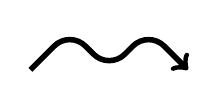
\begin{tikzpicture}[x=1mm,y=1mm]
  \draw[line width=2pt, rounded corners=8pt, ->]
  (0,0) -- (5,5) -- (10,0) -- (15,5) -- (20,0);
\end{tikzpicture}
が描かれる。
矢印は \verb'->'、\verb'<-'、\verb'<->'、\verb'->>' などが指定できる。
また、矢印の形には Ti\textit{k}Z 標準(
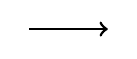
\begin{tikzpicture}[line width=1pt]
  \draw[->] (0,1) -- (1,1);
\end{tikzpicture}
)、\LaTeX{}標準(
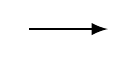
\begin{tikzpicture}[line width=1pt]
  \draw[-latex] (0,0.5) -- (1,0.5);
\end{tikzpicture}
)、ステルス戦闘機型(
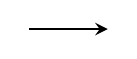
\begin{tikzpicture}[line width=1pt]
  \draw[-stealth] (0,0) -- (1,0);
\end{tikzpicture}
)などが用意されている。
\vspc{+0.50zw}\begin{mdframed}[roundcorner=0.50zw,leftmargin=3.00zw,rightmargin=3.00zw,skipabove=0.40zw,skipbelow=0.40zw,innertopmargin=4.00pt,innerbottommargin=4.00pt,innerleftmargin=5.00pt,innerrightmargin=5.00pt,linecolor=gray!020,linewidth=0.50pt,backgroundcolor=gray!20]
\begin{verbatim}
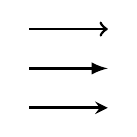
\begin{tikzpicture}[line width=1pt]
  \draw[->] (0,1) -- (1,1);
  \draw[-latex] (0,0.5) -- (1,0.5);
  \draw[-stealth] (0,0) -- (1,0);
\end{tikzpicture}
\end{verbatim}
\end{mdframed}\vspc{-0.70zw}
Ti\textit{k}Z 標準は、数式で $f:A \to B$ と書く際の \verb'\to'(\verb'\rightarrow')と(大きさは異なるが)同じ形である。\\

\verb'\draw' でグリッドや円、長方形、楕円も描くことができる。
勿論、日本語や数式も書くことができる。
\verb'\fill' にすると、指定した色で塗りつぶす(この例では 20\% の灰色)。
\vspc{+0.50zw}\begin{mdframed}[roundcorner=0.50zw,leftmargin=3.00zw,rightmargin=3.00zw,skipabove=0.40zw,skipbelow=0.40zw,innertopmargin=4.00pt,innerbottommargin=4.00pt,innerleftmargin=5.00pt,innerrightmargin=5.00pt,linecolor=gray!020,linewidth=0.50pt,backgroundcolor=gray!20]
\begin{verbatim}
\begin{tikzpicture}
  \draw[step=1,gray] (-0.2,-0.2) grid (2.2,2.2);
  \draw (0.5,0.5) circle (0.5) node {$\pi r^{2}$};
  \draw[line width=1pt] (1,0) rectangle (2,0.5);
  \fill[black!20] (1,1.5) ellipse (1 and 0.5);
  \draw (1,1.5) node {\hbox{\tate 楕円}};
\end{tikzpicture}
\end{verbatim}
\end{mdframed}\vspc{-0.70zw}
出力は次のようになる\\
\vspc{-2.50zw}\begin{center}
  \begin{tikzpicture}
    \draw[step=1,gray] (-0.2,-0.2) grid (2.2,2.2);
    \draw (0.5,0.5) circle (0.5) node {$\pi r^{2}$};
    \draw[line width=1pt] (1,0) rectangle (2,0.5);
    \fill[black!20] (1,1.5) ellipse (1 and 0.5);
    \draw (1,1.5) node {\hbox{\tate 楕円}};
  \end{tikzpicture}
\end{center}\vspc{-1.50zw}
より複雑な図形は、制御点を2つ与えたベジェ(B\'{e}zier)曲線で描くことができる。\enlargethispage{+0.90zw}
第 2 の制御点が第 1 のものと同じ場合は省略することができる。
\vspc{+0.50zw}\begin{mdframed}[roundcorner=0.50zw,leftmargin=3.00zw,rightmargin=3.00zw,skipabove=0.40zw,skipbelow=0.40zw,innertopmargin=4.00pt,innerbottommargin=4.00pt,innerleftmargin=5.00pt,innerrightmargin=5.00pt,linecolor=gray!020,linewidth=0.50pt,backgroundcolor=gray!20]
\begin{verbatim}
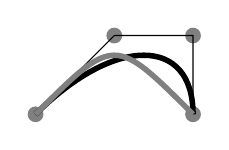
\begin{tikzpicture}[x=1mm,y=1mm]
  \fill[gray] ( 0, 0) circle (1)
              (10,10) circle (1)
              (20,10) circle (1)
              (20, 0) circle (1);
  \draw (0,0) -- (10,10) -- (20,10) -- (20,0);
  \draw[line width=2pt] (0,0) .. controls (10,10) and (20,10) .. (20,0);
  \draw[line width=2pt,gray] (0,0) .. controls (10,10) .. (20,0);
\end{tikzpicture}
\end{verbatim}
\end{mdframed}\vspc{-0.70zw}
出力は次のようになる。
\vspc{-1.50zw}\begin{center}
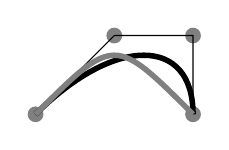
\begin{tikzpicture}[x=1mm,y=1mm]
  \fill[gray] ( 0, 0) circle (1)
              (10,10) circle (1)
              (20,10) circle (1)
              (20, 0) circle (1);
  \draw (0,0) -- (10,10) -- (20,10) -- (20,0);
  \draw[line width=2pt] (0,0) .. controls (10,10) and (20,10) .. (20,0);
  \draw[line width=2pt,gray] (0,0) .. controls (10,10) .. (20,0);
\end{tikzpicture}
\end{center}\vspc{-1.00zw}
折れ線と曲線は次のように混在させることができる。
\vspc{+0.00zw}\begin{mdframed}[roundcorner=0.50zw,leftmargin=3.00zw,rightmargin=3.00zw,skipabove=0.40zw,skipbelow=0.40zw,innertopmargin=4.00pt,innerbottommargin=4.00pt,innerleftmargin=5.00pt,innerrightmargin=5.00pt,linecolor=gray!020,linewidth=0.50pt,backgroundcolor=gray!20]
\begin{verbatim}

\begin{tikzpicture}[x=1mm,y=1mm,line width=2pt]
  \draw ( 2,2) circle (2);
  \draw ( 2,4) -- (6,4) -- ( 6,0) .. controls (6,3) and (7,4) ..
        (12,4) -- (9,0) -- (12,0);
\end{tikzpicture}
\end{verbatim}
\end{mdframed}\vspc{-0.70zw}
出力は次のようになる。
\vspc{-1.00zw}\begin{center}
  
\begin{tikzpicture}[x=1mm,y=1mm,line width=2pt]
    \draw (2,2) circle (2);
    \draw (2,4) -- (6,4) -- (6,0) .. controls (6,3) and (7,4) .. (12,4) -- (9,0) -- (12,0);
  \end{tikzpicture}
\end{center}\vspc{-1.00zw}
繰り返しも \verb'\foreach' という強力な命令で簡単に実現できる。
\verb'...' は書くのを省略したのではなく、本当にこのように記述すれば Ti\textit{k}Z が補ってくれる。
\vspc{+0.50zw}\begin{mdframed}[roundcorner=0.50zw,leftmargin=3.00zw,rightmargin=3.00zw,skipabove=0.40zw,skipbelow=0.40zw,innertopmargin=4.00pt,innerbottommargin=4.00pt,innerleftmargin=5.00pt,innerrightmargin=5.00pt,linecolor=gray!020,linewidth=0.50pt,backgroundcolor=gray!20]
\begin{verbatim}
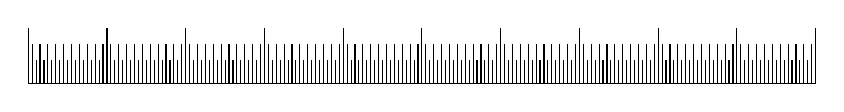
\begin{tikzpicture}[x=1mm,y=1mm]
  \draw (0,0) -- (100,0);
  \foreach \x in {0.0,...,100}    \draw (\x,0) -- (\x,3);
  \foreach \x in {0.5,...,100}    \draw (\x,0) -- (\x,5);
  \foreach \x in {0.0,10,...,100} \draw (\x,0) -- (\x,7);
\end{tikzpicture}
\end{verbatim}
\end{mdframed}\vspc{-0.70zw}
出力は次のようになる。
\vspc{-0.50zw}\begin{center}
  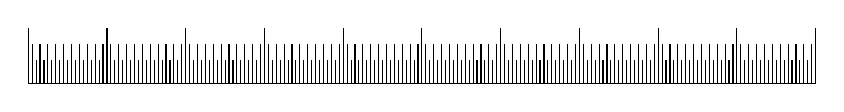
\begin{tikzpicture}[x=1mm,y=1mm]
  \draw (0,0) -- (100,0);
  \foreach \x in {0.0,...,100}    \draw (\x,0) -- (\x,3);
  \foreach \x in {0.5,...,100}    \draw (\x,0) -- (\x,5);
  \foreach \x in {0.0,10,...,100} \draw (\x,0) -- (\x,7);
\end{tikzpicture}
\end{center}\vspc{-0.50zw}
応用として、センター試験でよく使われる楕円の番号を作成してみる。
\vspc{+0.50zw}\begin{mdframed}[roundcorner=0.50zw,leftmargin=3.00zw,rightmargin=3.00zw,skipabove=0.40zw,skipbelow=0.40zw,innertopmargin=4.00pt,innerbottommargin=4.00pt,innerleftmargin=5.00pt,innerrightmargin=5.00pt,linecolor=gray!020,linewidth=0.50pt,backgroundcolor=gray!20]
\begin{verbatim}
\newcommand{\egg}[1]{\raisebox{-3pt}{%
    \begin{tikzpicture}[x=1pt,y=1pt,line width=1pt]
      \draw (0,0) ellipse (4.5 and 6);
      \draw (0,0) node {\fontfamily{phv}\fontsize{9pt}{0}\selectfont #1\/};
    \end{tikzpicture}}}
\newcommand{\eggg}[1]{\raisebox{-3pt}{%
    \begin{tikzpicture}[x=1pt,y=1pt,line width=1pt]
      \draw[fill=black!30] (0,0) ellipse (4.5 and 6);
      \draw (0,0) node {\fontfamily{phv}\fontsize{9pt}{0}\selectfont #1\/};
    \end{tikzpicture}}}
\end{verbatim}
\end{mdframed}\vspc{-0.70zw}
\newcommand{\egg}[1]{\raisebox{-3pt}{%
    \begin{tikzpicture}[x=1pt,y=1pt,line width=1pt]
      \draw (0,0) ellipse (4.5 and 6);
      \draw (0,0) node {\fontfamily{phv}\fontsize{9pt}{0}\selectfont #1\/};
    \end{tikzpicture}}}
\newcommand{\eggg}[1]{\raisebox{-3pt}{%
    \begin{tikzpicture}[x=1pt,y=1pt,line width=1pt]
      \draw[fill=black!30] (0,0) ellipse (4.5 and 6);
      \draw (0,0) node {\fontfamily{phv}\fontsize{9pt}{0}\selectfont #1\/};
    \end{tikzpicture}}}
これで \verb'\egg{0} \egg{1} \egg{2} \eggg{0} \eggg{1} \eggg{2}' とすれば \egg{0} \egg{1} \egg{2} \eggg{0} \eggg{1} \eggg{2} と出力される。\\
\renewcommand{\keytop}[2][12]{%
  \begin{tikzpicture}[x=0.1em,y=0.1em]
    \useasboundingbox (0,0) rectangle (#1,9);
    \shadedraw[top color=black!20,rounded corners=0.2em] (0,-3) rectangle (#1,9);
    \draw[anchor=base] (#1/2,0) node {\sffamily #2};
  \end{tikzpicture}}
次は \keytop{A} のようなキーボード記号である。
\vspc{+0.50zw}\begin{mdframed}[roundcorner=0.50zw,leftmargin=3.00zw,rightmargin=3.00zw,skipabove=0.40zw,skipbelow=0.40zw,innertopmargin=4.00pt,innerbottommargin=4.00pt,innerleftmargin=5.00pt,innerrightmargin=5.00pt,linecolor=gray!020,linewidth=0.50pt,backgroundcolor=gray!20]
\begin{verbatim}
\renewcommand{\keytop}[2][12]{%
  \begin{tikzpicture}[x=0.1em,y=0.1em]
    \useasboundingbox (0,0) rectangle (#1,9);
    \shadedraw[top color=black!20,rounded corners=0.2em] (0,-3)
    rectangle (#1,9);
    \draw[anchor=base] (#1/2,0) node {\sffamily #2};
\end{verbatim}
\end{mdframed}\vspc{-0.70zw}
\verb'\keytop{A}' と書けば \keytop{A} と出力される。
\keytop[30]{Enter} のように幅の広いものは \verb'\ketop[30]{Enter}' のように幅を 0.1em 単位で指定する。\enlargethispage{+1.00zw}
%%
%% 節:グラフの描画(1)
%%--------------------------------------------------------------------------------------------------------------------%%
\section{グラフの描画(1)}
Ti\textit{k}Z では \textrm{sin}、\textrm{cos}、\textrm{exp}、\textrm{sqrt} などの関数が利用できる。
但し、TeX{}で実装しているので、遅く、精度の低い固定小数点数である。
次のような簡単なことは可能である。
\vspc{+0.50zw}\begin{mdframed}[roundcorner=0.50zw,leftmargin=3.00zw,rightmargin=3.00zw,skipabove=0.40zw,skipbelow=0.40zw,innertopmargin=4.00pt,innerbottommargin=4.00pt,innerleftmargin=5.00pt,innerrightmargin=5.00pt,linecolor=gray!020,linewidth=0.50pt,backgroundcolor=gray!20]
\begin{verbatim}
\begin{tikzpicture}[domain=0:4,samples=200,>=stealth]
  \draw[->] (-0.5,0) -- (4.2,0) node[right] {$x$};
  \draw[->] (0,-0.5) -- (0,2.2) node[above] {$y$};
  \draw plot (\x, {sqrt(\x)}) node[below] {$y=\sqrt{x}$};
  \draw (0,0) node[below left] {O};
\end{tikzpicture}
\end{verbatim}
\end{mdframed}\vspc{-0.70zw}
出力は次のようになる。
\vspc{-0.50zw}\begin{center}
  \begin{tikzpicture}[domain=0:4,samples=200,>=stealth]
    \draw[->] (-0.5,0) -- (4.2,0) node[right] {$x$};
    \draw[->] (0,-0.5) -- (0,2.2) node[above] {$y$};
    \draw plot (\x, {sqrt(\x)}) node[below] {$y=\sqrt{x}$};
    \draw (0,0) node[below left] {O};
  \end{tikzpicture}
\end{center}\vspc{-0.50zw}
数値の表を与えてグラフをプロットすることもできる。
例えば、毎年の日本の合計特殊出生率が、
\vspc{-0.50zw}\begin{quote}
  1970 2.13 \\
  1971 2.16 \\
  1972 2.14 \\
  $\ldots$  \\
  2015 1.46
\end{quote}\vspc{-0.50zw}
のようなテキストファイル TFR.tbl で与えられているとする。
これを、
\begin{center}
  \begin{tikzpicture}[x=2mm,y=40mm]
    \draw (1968,1.2) -- (1968,2.2);
    \foreach \x in {1.2,1.4,1.6,1.8,2.0,2.2}
    \draw (1968,\x) -- (1967,\x) node[left] {\x};
    \draw (1970,1.1) -- (2015,1.1);
    \foreach \x in {1970,1980,...,2000,2010,2015}
    \draw (\x,1.1) -- (\x,1.05) node[below] {\x};
    \draw[mark=*] plot file {./Fig/TFR.tbl} node[above] {1.46};
  \end{tikzpicture}
\end{center}\vspc{-0.50zw}
のように描くには次のようにする。\enlargethispage{+0.50zw}
\vspc{+0.50zw}\begin{mdframed}[roundcorner=0.50zw,leftmargin=3.00zw,rightmargin=3.00zw,skipabove=0.40zw,skipbelow=0.40zw,innertopmargin=4.00pt,innerbottommargin=4.00pt,innerleftmargin=5.00pt,innerrightmargin=5.00pt,linecolor=gray!020,linewidth=0.50pt,backgroundcolor=gray!20]
\begin{verbatim}
\begin{tikzpicture}[x=2mm,y=40mm]
  \draw (1968,1.2) -- (1968,2.2);
  \foreach \x in {1.2,1.4,1.6,1.8,2.0,2.2}
  \draw (1968,\x) -- (1967,\x) node[left] {\x};
  \draw (1970,1.1) -- (2015,1.1);
  \foreach \x in {1970,1980,...,2000,2010,2015}
  \draw (\x,1.1) -- (\x,1.05) node[below] {\x};
  \draw[mark=*] plot file {TFR.tbl} node[above] {1.46};
\end{tikzpicture}
\end{verbatim}
\end{mdframed}\vspc{-0.50zw}
あるいは、もっと単純に
\begin{tikzpicture}[x=1pt]
  \fill (1970,2.13) circle (2pt) node[left] {2.13};
  \draw plot file {./Fig/TFR.tbl};
  \fill (2015,1.46) circle (2pt) node[right] {1.46};
\end{tikzpicture}
のようなスパークライン(sparkline)で描くには次のようにする。
\vspc{-1.00zw}\begin{mdframed}[roundcorner=0.50zw,leftmargin=3.00zw,rightmargin=3.00zw,skipabove=0.40zw,skipbelow=0.40zw,innertopmargin=4.00pt,innerbottommargin=4.00pt,innerleftmargin=5.00pt,innerrightmargin=5.00pt,linecolor=gray!020,linewidth=0.50pt,backgroundcolor=gray!20]
\begin{verbatim}
\begin{tikzpicture}[x=1pt]
  \fill (1970,2.13) circle (2pt) node[left] {2.13};
  \draw plot file {TFR.tbl};
  \fill (2015,1.46) circle (2pt) node[right] {1.46};
\end{tikzpicture}
\end{verbatim}
\end{mdframed}\vspc{-0.70zw}
但し、Ti\textit{k}Z は\TeX{}の固定小数点数で計算するので、あまり大きな値を扱うと ``ERROR:~Dimension too large.'' となることがある。
その場合は、適当に数値を切り詰める。\\

次の棒グラフの例では、年から 2000 を引いた値を$x$座標としている。
\vspc{+0.50zw}\begin{mdframed}[roundcorner=0.50zw,leftmargin=3.00zw,rightmargin=3.00zw,skipabove=0.40zw,skipbelow=0.40zw,innertopmargin=4.00pt,innerbottommargin=4.00pt,innerleftmargin=5.00pt,innerrightmargin=5.00pt,linecolor=gray!020,linewidth=0.50pt,backgroundcolor=gray!20]
\begin{verbatim}
\begin{tikzpicture}[ybar,x=5mm,y=0.005mm]
  \draw[fill=lightgray] plot coordinates
  {( 4,12415) ( 5,12317) ( 6,12214) ( 7,12043) ( 8,11813) ( 9,11695)
   (10,11585) (11,11528) (12,11366) (13,10792) (14,11123) (15,10945)};
  \draw (4,0) node[below] {2004};
  \draw (15,0) node[below] {2015};
  \draw (4,12315)|-(16,13000) node[right] {12415億円};
  \draw (15,10945)|-(16,12000) node[right] {10945億円};
  \draw (9.5,13000) node[above] {\large 国立大学運営費交付金};
\end{tikzpicture}
\end{verbatim}
\end{mdframed}\vspc{-0.70zw}
この例では、引出線を引くために \verb'--' ではなく \verb'|-' を使っている。
$(x_{1},y_{1})$ \verb'|-' $(x_{2},y_{2})$ は $(x_{1},y_{1})$ \verb'--' $(x_{1},y_{2})$ \verb'--' $(x_{2},y_{2})$ と同じことで、先に水平方向に、次に水平方向に線を引く。
水平と垂直の順序を入れ替えた \verb'-|' も用意されている。
\vspc{+0.50zw}\begin{center}
  \begin{tikzpicture}[ybar,x=5mm,y=0.005mm]
    \draw[fill=lightgray] plot coordinates
    {( 4,12415) ( 5,12317) ( 6,12214) ( 7,12043) ( 8,11813) ( 9,11695)
     (10,11585) (11,11528) (12,11366) (13,10792) (14,11123) (15,10945)};
    \draw (4,0) node[below] {2004};
    \draw (15,0) node[below] {2015};
    \draw (4,12315)|-(16,13000) node[right] {12415億円};
    \draw (15,10945)|-(16,12000) node[right] {10945億円};
    \draw (9.5, 13000) node[above] {\large 国立大学運営費交付金};
  \end{tikzpicture}
\end{center}\vspc{-0.70zw}
%%
%% 節:グラフの描画(2)
%%--------------------------------------------------------------------------------------------------------------------%%
\section{グラフの描画(2)}
グラフと言えば、グラフ理論のグラフも簡単に描くことができる。
ノード(点)に名前を付け、両端のノードを指定して辺を描けばよい。
次のグラフは、有名な \ruby{K\"{o}nigsberg}{ケーニヒスベルク} の橋の問題のグラフである。
\vspc{+0.50zw}\begin{mdframed}[roundcorner=0.50zw,leftmargin=3.00zw,rightmargin=3.00zw,skipabove=0.40zw,skipbelow=0.40zw,innertopmargin=4.00pt,innerbottommargin=4.00pt,innerleftmargin=5.00pt,innerrightmargin=5.00pt,linecolor=gray!020,linewidth=0.50pt,backgroundcolor=gray!20]
\begin{verbatim}
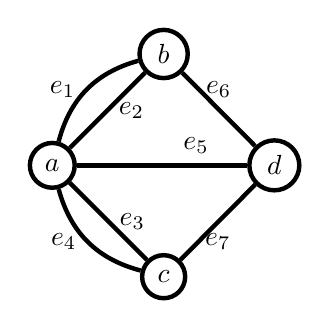
\begin{tikzpicture}[line width=1.6pt,node distance=2cm]
  \node(a) [draw,circle]{$a$};
  \node[above right of=a](b)                [draw,circle]{$b$};
  \node[below right of=a](c)                [draw,circle]{$c$};
  \node[right of=a,node distance=2.82cm](d) [draw,circle]{$d$};
  \draw (a) to[bend left]  node[midway,left]  {$e_{1}$} (b);
  \draw (a) --             node[midway,right] {$e_{2}$} (b);
  \draw (a) --             node[midway,right] {$e_{3}$} (c);
  \draw (a) to[bend right] node[midway,left]  {$e_{4}$} (c);
  \draw (a) --             node[pos=.7,above] {$e_{5}$} (d);
  \draw (b) --             node[midway,above] {$e_{6}$} (d);
  \draw (c) --             node[midway,below] {$e_{7}$} (d);
\end{tikzpicture}
\end{verbatim}
\end{mdframed}\vspc{-0.70zw}
\begin{center}
  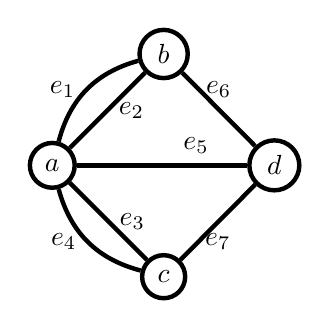
\begin{tikzpicture}[line width=1.6pt,node distance=2cm]
  \node(a) [draw,circle]{$a$};
  \node[above right of=a](b)                [draw,circle]{$b$};
  \node[below right of=a](c)                [draw,circle]{$c$};
  \node[right of=a,node distance=2.82cm](d) [draw,circle]{$d$};
  \draw (a) to[bend left]  node[midway,left]  {$e_{1}$} (b);
  \draw (a) --             node[midway,right] {$e_{2}$} (b);
  \draw (a) --             node[midway,right] {$e_{3}$} (c);
  \draw (a) to[bend right] node[midway,left]  {$e_{4}$} (c);
  \draw (a) --             node[pos=.7,above] {$e_{5}$} (d);
  \draw (b) --             node[midway,above] {$e_{6}$} (d);
  \draw (c) --             node[midway,below] {$e_{7}$} (d);
  \end{tikzpicture}
\end{center}
この例では、ノード$a$を基準とした相対的な位置で$b$、$c$、$d$を指定している。
辺は両端点で指定し、辺の途中にラベルを付けている。
bend left や bend right で湾曲した辺を描くには \verb'--'ではなく to を用いる(この例では \verb'--' を全て to に置き換えても構わない)。
%%
%% 節:gnuplot との連携
%%--------------------------------------------------------------------------------------------------------------------%%
\section{gnuplot との連携}
\ruby{gnuplot}{ニュープロット}\footnote{GNU プロジェクトを思わせる名前なのでグニュ―プロットと呼ばれることもあるが、GNU プロジェクトとは無関係である。} は昔から使われている強力なプロットツールである。
これと連携させて Ti\textit{k}Z のプロットを描くことができる。
例えば、標準正規分布のグラフを描いてみる。
次のように \verb'function{...}' という命令を使えば、関数の中身 \verb'exp(-x**2/2)/sqrt(2*pi)' が gnuplot に渡され、関数値の表に変換される。
この際、platex に \verb'-shell-escape' オプションを付けて起動しなければならない。
gnuplot で渡される命令と、返される表のファイル名は\LaTeX{}文書のファイル名と \verb'-id=' で与えられた名前から生成される。
一旦これらが生成されれば、関数を変えない限り gnuplot を呼び出すことはないので \verb'-shell-escape' オプションも不要である。\\
\vspc{-1.00zw}\begin{mdframed}[roundcorner=0.50zw,leftmargin=3.00zw,rightmargin=3.00zw,skipabove=0.40zw,skipbelow=0.40zw,innertopmargin=4.00pt,innerbottommargin=4.00pt,innerleftmargin=5.00pt,innerrightmargin=5.00pt,linecolor=gray!020,linewidth=0.50pt,backgroundcolor=gray!20]
\begin{verbatim}
\begin{tikzpicture}[domain=-3:3,samples=50,>=latex,y=8cm]
  \draw[->] (-3.2,0) -- (3.2,0) node[right] {$x$};
  \draw plot[id=dnorm,smooth] function{exp(-x**2/2)/sqrt(2*pi)};
  \draw (2,0.35) node {$y=\frac{1}{\sqrt{2\pi}}e^{-x^{2}\!\/2}$};
  \foreach \x in {-3,...,3}
  \draw (\x,0) -- (\x,-0.02) node[below=-2pt] {\footnotesize $\x$};
\end{tikzpicture}
\end{verbatim}
\end{mdframed}\vspc{-0.70zw}
\begin{center}
  \begin{tikzpicture}[domain=-3:3,samples=50,>=latex,y=8cm]
    \draw[->] (-3.2,0) -- (3.2,0) node[right] {$x$};
    \draw plot[id=dnorm,smooth] function{exp(-x**2/2)/sqrt(2*pi)};
    \draw (2,0.35) node {$y=\frac{1}{\sqrt{2\pi}}e^{-x^{2}\!\/2}$};
    \foreach \x in {-3,...,3}
    \draw (\x,0) -- (\x,-0.02) node[below=-2pt] {\footnotesize $\x$};
  \end{tikzpicture}
\end{center}
尚、これぐらいの関数であれば、Ti\textit{k}Z だけで、
\vspc{+0.50zw}\begin{mdframed}[roundcorner=0.50zw,leftmargin=3.00zw,rightmargin=3.00zw,skipabove=0.40zw,skipbelow=0.40zw,innertopmargin=4.00pt,innerbottommargin=4.00pt,innerleftmargin=5.00pt,innerrightmargin=5.00pt,linecolor=gray!020,linewidth=0.50pt,backgroundcolor=gray!20]
\begin{verbatim}
\draw plot[smooth] (\x, {exp(-0.5 * \x \x) / sqrt(2 * pi)});
\end{verbatim}
\end{mdframed}\vspc{-0.70zw}
のようにして描くこともできる。\\

gnuplot から返される表は、\# で始まるコメント行を除けば、次のような形式である。
\vspc{+0.50zw}\begin{mdframed}[roundcorner=0.50zw,leftmargin=3.00zw,rightmargin=3.00zw,skipabove=0.40zw,skipbelow=0.40zw,innertopmargin=4.00pt,innerbottommargin=4.00pt,innerleftmargin=5.00pt,innerrightmargin=5.00pt,linecolor=gray!020,linewidth=0.50pt,backgroundcolor=gray!20]
\begin{verbatim}
  -3.00000 0.00443 i
  -2.87755 0.00635 i
  -2.75510 0.00897 i
  ...
\end{verbatim}
\end{mdframed}\vspc{-0.70zw}
最後の文字 i は範囲内、o は範囲外、u は未定義を表す。\enlargethispage{+0.60zw}
gnuplot に関わらず、このような表を用意しておけば、
\vspc{+0.50zw}\begin{mdframed}[roundcorner=0.50zw,leftmargin=3.00zw,rightmargin=3.00zw,skipabove=0.40zw,skipbelow=0.40zw,innertopmargin=4.00pt,innerbottommargin=4.00pt,innerleftmargin=5.00pt,innerrightmargin=5.00pt,linecolor=gray!020,linewidth=0.50pt,backgroundcolor=gray!20]
\begin{verbatim}
\draw plot[smooth] file {ファイル名};
\end{verbatim}
\end{mdframed}\vspc{-0.70zw}
のようにしてプロットすることができる。

別の方法として gnuplot で、
\vspc{+0.50zw}\begin{mdframed}[roundcorner=0.50zw,leftmargin=3.00zw,rightmargin=3.00zw,skipabove=0.40zw,skipbelow=0.40zw,innertopmargin=4.00pt,innerbottommargin=4.00pt,innerleftmargin=5.00pt,innerrightmargin=5.00pt,linecolor=gray!020,linewidth=0.50pt,backgroundcolor=gray!20]
\begin{verbatim}
set term tikz
\end{verbatim}
\end{mdframed}\vspc{-0.70zw}
とすれば、Ti\textit{k}Z 形式の出力が得られる。
例えば、
\vspc{+0.50zw}\begin{mdframed}[roundcorner=0.50zw,leftmargin=3.00zw,rightmargin=3.00zw,skipabove=0.40zw,skipbelow=0.40zw,innertopmargin=4.00pt,innerbottommargin=4.00pt,innerleftmargin=5.00pt,innerrightmargin=5.00pt,linecolor=gray!020,linewidth=0.50pt,backgroundcolor=gray!20]
\begin{verbatim}
set term tikz monochrome
set output "dnorm-gp.tex"
set xrange [-3:3]
plot exp(-x**2/2)/sqrt(2*pi) with lines
exit
\end{verbatim}
\end{mdframed}\vspc{-0.70zw}
とし、\LaTeX{}文書の中では、
\vspc{+0.50zw}\begin{mdframed}[roundcorner=0.50zw,leftmargin=3.00zw,rightmargin=3.00zw,skipabove=0.40zw,skipbelow=0.40zw,innertopmargin=4.00pt,innerbottommargin=4.00pt,innerleftmargin=5.00pt,innerrightmargin=5.00pt,linecolor=gray!020,linewidth=0.50pt,backgroundcolor=gray!20]
\begin{verbatim}
\documentclass[dvipdfmx]{jsarticle}
\usepackage{gnuplot-lua-tikz}
\begin{document}
\begin{tikzpicture}[gnuplot]
%% generated with GNUPLOT 5.2p8 (Lua 5.3; terminal rev. Nov 2018, script rev. 108)
%% 2020年09月17日 09時41分47秒
\path (0.000,0.000) rectangle (12.500,8.750);
\gpcolor{color=gp lt color border}
\gpsetlinetype{gp lt border}
\gpsetdashtype{gp dt solid}
\gpsetlinewidth{1.00}
\draw[gp path] (1.196,0.616)--(1.376,0.616);
\draw[gp path] (11.947,0.616)--(11.767,0.616);
\node[gp node right] at (1.012,0.616) {$0$};
\draw[gp path] (1.196,1.594)--(1.376,1.594);
\draw[gp path] (11.947,1.594)--(11.767,1.594);
\node[gp node right] at (1.012,1.594) {$0.05$};
\draw[gp path] (1.196,2.572)--(1.376,2.572);
\draw[gp path] (11.947,2.572)--(11.767,2.572);
\node[gp node right] at (1.012,2.572) {$0.1$};
\draw[gp path] (1.196,3.550)--(1.376,3.550);
\draw[gp path] (11.947,3.550)--(11.767,3.550);
\node[gp node right] at (1.012,3.550) {$0.15$};
\draw[gp path] (1.196,4.529)--(1.376,4.529);
\draw[gp path] (11.947,4.529)--(11.767,4.529);
\node[gp node right] at (1.012,4.529) {$0.2$};
\draw[gp path] (1.196,5.507)--(1.376,5.507);
\draw[gp path] (11.947,5.507)--(11.767,5.507);
\node[gp node right] at (1.012,5.507) {$0.25$};
\draw[gp path] (1.196,6.485)--(1.376,6.485);
\draw[gp path] (11.947,6.485)--(11.767,6.485);
\node[gp node right] at (1.012,6.485) {$0.3$};
\draw[gp path] (1.196,7.463)--(1.376,7.463);
\draw[gp path] (11.947,7.463)--(11.767,7.463);
\node[gp node right] at (1.012,7.463) {$0.35$};
\draw[gp path] (1.196,8.441)--(1.376,8.441);
\draw[gp path] (11.947,8.441)--(11.767,8.441);
\node[gp node right] at (1.012,8.441) {$0.4$};
\draw[gp path] (1.196,0.616)--(1.196,0.796);
\draw[gp path] (1.196,8.441)--(1.196,8.261);
\node[gp node center] at (1.196,0.308) {$-3$};
\draw[gp path] (2.988,0.616)--(2.988,0.796);
\draw[gp path] (2.988,8.441)--(2.988,8.261);
\node[gp node center] at (2.988,0.308) {$-2$};
\draw[gp path] (4.780,0.616)--(4.780,0.796);
\draw[gp path] (4.780,8.441)--(4.780,8.261);
\node[gp node center] at (4.780,0.308) {$-1$};
\draw[gp path] (6.572,0.616)--(6.572,0.796);
\draw[gp path] (6.572,8.441)--(6.572,8.261);
\node[gp node center] at (6.572,0.308) {$0$};
\draw[gp path] (8.363,0.616)--(8.363,0.796);
\draw[gp path] (8.363,8.441)--(8.363,8.261);
\node[gp node center] at (8.363,0.308) {$1$};
\draw[gp path] (10.155,0.616)--(10.155,0.796);
\draw[gp path] (10.155,8.441)--(10.155,8.261);
\node[gp node center] at (10.155,0.308) {$2$};
\draw[gp path] (11.947,0.616)--(11.947,0.796);
\draw[gp path] (11.947,8.441)--(11.947,8.261);
\node[gp node center] at (11.947,0.308) {$3$};
\draw[gp path] (1.196,8.441)--(1.196,0.616)--(11.947,0.616)--(11.947,8.441)--cycle;
\node[gp node right] at (10.479,8.107) {exp(-x**2/2)/sqrt(2*pi)};
\draw[gp path] (10.663,8.107)--(11.579,8.107);
\draw[gp path] (1.196,0.703)--(1.305,0.720)--(1.413,0.740)--(1.522,0.763)--(1.630,0.790)%
  --(1.739,0.822)--(1.848,0.858)--(1.956,0.899)--(2.065,0.946)--(2.173,1.000)--(2.282,1.061)%
  --(2.391,1.129)--(2.499,1.206)--(2.608,1.292)--(2.716,1.387)--(2.825,1.493)--(2.934,1.610)%
  --(3.042,1.738)--(3.151,1.878)--(3.259,2.030)--(3.368,2.194)--(3.477,2.372)--(3.585,2.562)%
  --(3.694,2.765)--(3.802,2.980)--(3.911,3.208)--(4.019,3.446)--(4.128,3.696)--(4.237,3.955)%
  --(4.345,4.223)--(4.454,4.498)--(4.562,4.779)--(4.671,5.063)--(4.780,5.350)--(4.888,5.636)%
  --(4.997,5.920)--(5.105,6.200)--(5.214,6.473)--(5.323,6.737)--(5.431,6.990)--(5.540,7.228)%
  --(5.648,7.451)--(5.757,7.654)--(5.866,7.838)--(5.974,7.999)--(6.083,8.135)--(6.191,8.247)%
  --(6.300,8.331)--(6.409,8.388)--(6.517,8.417)--(6.626,8.417)--(6.734,8.388)--(6.843,8.331)%
  --(6.952,8.247)--(7.060,8.135)--(7.169,7.999)--(7.277,7.838)--(7.386,7.654)--(7.495,7.451)%
  --(7.603,7.228)--(7.712,6.990)--(7.820,6.737)--(7.929,6.473)--(8.038,6.200)--(8.146,5.920)%
  --(8.255,5.636)--(8.363,5.350)--(8.472,5.063)--(8.581,4.779)--(8.689,4.498)--(8.798,4.223)%
  --(8.906,3.955)--(9.015,3.696)--(9.124,3.446)--(9.232,3.208)--(9.341,2.980)--(9.449,2.765)%
  --(9.558,2.562)--(9.666,2.372)--(9.775,2.194)--(9.884,2.030)--(9.992,1.878)--(10.101,1.738)%
  --(10.209,1.610)--(10.318,1.493)--(10.427,1.387)--(10.535,1.292)--(10.644,1.206)--(10.752,1.129)%
  --(10.861,1.061)--(10.970,1.000)--(11.078,0.946)--(11.187,0.899)--(11.295,0.858)--(11.404,0.822)%
  --(11.513,0.790)--(11.621,0.763)--(11.730,0.740)--(11.838,0.720)--(11.947,0.703);
\draw[gp path] (1.196,8.441)--(1.196,0.616)--(11.947,0.616)--(11.947,8.441)--cycle;
%% coordinates of the plot area
\gpdefrectangularnode{gp plot 1}{\pgfpoint{1.196cm}{0.616cm}}{\pgfpoint{11.947cm}{8.441cm}}
\end{tikzpicture}
%% gnuplot variables

\end{document}
\end{verbatim}
\end{mdframed}\vspc{-0.70zw}
とすれば、下のような図が得られる。
実際には、更に手を加えて見栄えを良くする必要がある。
\begin{center}
  \begin{tikzpicture}[gnuplot]
%% generated with GNUPLOT 5.2p8 (Lua 5.3; terminal rev. Nov 2018, script rev. 108)
%% 2020年09月17日 09時41分47秒
\path (0.000,0.000) rectangle (12.500,8.750);
\gpcolor{color=gp lt color border}
\gpsetlinetype{gp lt border}
\gpsetdashtype{gp dt solid}
\gpsetlinewidth{1.00}
\draw[gp path] (1.196,0.616)--(1.376,0.616);
\draw[gp path] (11.947,0.616)--(11.767,0.616);
\node[gp node right] at (1.012,0.616) {$0$};
\draw[gp path] (1.196,1.594)--(1.376,1.594);
\draw[gp path] (11.947,1.594)--(11.767,1.594);
\node[gp node right] at (1.012,1.594) {$0.05$};
\draw[gp path] (1.196,2.572)--(1.376,2.572);
\draw[gp path] (11.947,2.572)--(11.767,2.572);
\node[gp node right] at (1.012,2.572) {$0.1$};
\draw[gp path] (1.196,3.550)--(1.376,3.550);
\draw[gp path] (11.947,3.550)--(11.767,3.550);
\node[gp node right] at (1.012,3.550) {$0.15$};
\draw[gp path] (1.196,4.529)--(1.376,4.529);
\draw[gp path] (11.947,4.529)--(11.767,4.529);
\node[gp node right] at (1.012,4.529) {$0.2$};
\draw[gp path] (1.196,5.507)--(1.376,5.507);
\draw[gp path] (11.947,5.507)--(11.767,5.507);
\node[gp node right] at (1.012,5.507) {$0.25$};
\draw[gp path] (1.196,6.485)--(1.376,6.485);
\draw[gp path] (11.947,6.485)--(11.767,6.485);
\node[gp node right] at (1.012,6.485) {$0.3$};
\draw[gp path] (1.196,7.463)--(1.376,7.463);
\draw[gp path] (11.947,7.463)--(11.767,7.463);
\node[gp node right] at (1.012,7.463) {$0.35$};
\draw[gp path] (1.196,8.441)--(1.376,8.441);
\draw[gp path] (11.947,8.441)--(11.767,8.441);
\node[gp node right] at (1.012,8.441) {$0.4$};
\draw[gp path] (1.196,0.616)--(1.196,0.796);
\draw[gp path] (1.196,8.441)--(1.196,8.261);
\node[gp node center] at (1.196,0.308) {$-3$};
\draw[gp path] (2.988,0.616)--(2.988,0.796);
\draw[gp path] (2.988,8.441)--(2.988,8.261);
\node[gp node center] at (2.988,0.308) {$-2$};
\draw[gp path] (4.780,0.616)--(4.780,0.796);
\draw[gp path] (4.780,8.441)--(4.780,8.261);
\node[gp node center] at (4.780,0.308) {$-1$};
\draw[gp path] (6.572,0.616)--(6.572,0.796);
\draw[gp path] (6.572,8.441)--(6.572,8.261);
\node[gp node center] at (6.572,0.308) {$0$};
\draw[gp path] (8.363,0.616)--(8.363,0.796);
\draw[gp path] (8.363,8.441)--(8.363,8.261);
\node[gp node center] at (8.363,0.308) {$1$};
\draw[gp path] (10.155,0.616)--(10.155,0.796);
\draw[gp path] (10.155,8.441)--(10.155,8.261);
\node[gp node center] at (10.155,0.308) {$2$};
\draw[gp path] (11.947,0.616)--(11.947,0.796);
\draw[gp path] (11.947,8.441)--(11.947,8.261);
\node[gp node center] at (11.947,0.308) {$3$};
\draw[gp path] (1.196,8.441)--(1.196,0.616)--(11.947,0.616)--(11.947,8.441)--cycle;
\node[gp node right] at (10.479,8.107) {exp(-x**2/2)/sqrt(2*pi)};
\draw[gp path] (10.663,8.107)--(11.579,8.107);
\draw[gp path] (1.196,0.703)--(1.305,0.720)--(1.413,0.740)--(1.522,0.763)--(1.630,0.790)%
  --(1.739,0.822)--(1.848,0.858)--(1.956,0.899)--(2.065,0.946)--(2.173,1.000)--(2.282,1.061)%
  --(2.391,1.129)--(2.499,1.206)--(2.608,1.292)--(2.716,1.387)--(2.825,1.493)--(2.934,1.610)%
  --(3.042,1.738)--(3.151,1.878)--(3.259,2.030)--(3.368,2.194)--(3.477,2.372)--(3.585,2.562)%
  --(3.694,2.765)--(3.802,2.980)--(3.911,3.208)--(4.019,3.446)--(4.128,3.696)--(4.237,3.955)%
  --(4.345,4.223)--(4.454,4.498)--(4.562,4.779)--(4.671,5.063)--(4.780,5.350)--(4.888,5.636)%
  --(4.997,5.920)--(5.105,6.200)--(5.214,6.473)--(5.323,6.737)--(5.431,6.990)--(5.540,7.228)%
  --(5.648,7.451)--(5.757,7.654)--(5.866,7.838)--(5.974,7.999)--(6.083,8.135)--(6.191,8.247)%
  --(6.300,8.331)--(6.409,8.388)--(6.517,8.417)--(6.626,8.417)--(6.734,8.388)--(6.843,8.331)%
  --(6.952,8.247)--(7.060,8.135)--(7.169,7.999)--(7.277,7.838)--(7.386,7.654)--(7.495,7.451)%
  --(7.603,7.228)--(7.712,6.990)--(7.820,6.737)--(7.929,6.473)--(8.038,6.200)--(8.146,5.920)%
  --(8.255,5.636)--(8.363,5.350)--(8.472,5.063)--(8.581,4.779)--(8.689,4.498)--(8.798,4.223)%
  --(8.906,3.955)--(9.015,3.696)--(9.124,3.446)--(9.232,3.208)--(9.341,2.980)--(9.449,2.765)%
  --(9.558,2.562)--(9.666,2.372)--(9.775,2.194)--(9.884,2.030)--(9.992,1.878)--(10.101,1.738)%
  --(10.209,1.610)--(10.318,1.493)--(10.427,1.387)--(10.535,1.292)--(10.644,1.206)--(10.752,1.129)%
  --(10.861,1.061)--(10.970,1.000)--(11.078,0.946)--(11.187,0.899)--(11.295,0.858)--(11.404,0.822)%
  --(11.513,0.790)--(11.621,0.763)--(11.730,0.740)--(11.838,0.720)--(11.947,0.703);
\draw[gp path] (1.196,8.441)--(1.196,0.616)--(11.947,0.616)--(11.947,8.441)--cycle;
%% coordinates of the plot area
\gpdefrectangularnode{gp plot 1}{\pgfpoint{1.196cm}{0.616cm}}{\pgfpoint{11.947cm}{8.441cm}}
\end{tikzpicture}
%% gnuplot variables

\end{center}
%%
%% 節:他の図との重ね書き
%%--------------------------------------------------------------------------------------------------------------------%%
\section{他の図との重ね書き節}
Ti\textit{k}Z は強力な描画能力を備えているが、コマンドだけで全てを描くのは難しい。
そこで、他のソフトで描いた図の上に\TeX{}の数式などを Ti\textit{k}Z で重ね書きする方法を考える。
例えば、Ghostscript の虎の絵に説明を加えてみる。
図は、\enlargethispage{+0.50zw}
\vspc{-1.00zw}\begin{mdframed}[roundcorner=0.50zw,leftmargin=3.00zw,rightmargin=3.00zw,skipabove=0.40zw,skipbelow=0.40zw,innertopmargin=4.00pt,innerbottommargin=4.00pt,innerleftmargin=5.00pt,innerrightmargin=5.00pt,linecolor=gray!020,linewidth=0.50pt,backgroundcolor=gray!20]
\begin{verbatim}
\includegraphics[width=3cm]{tiger.pdf}
\end{verbatim}
\end{mdframed}\vspc{-0.70zw}
のような命令で読み込むのであった。\\

この任意の位置に文字や図を重ね書きするために、一時的にグラフ用紙を重ね書きしてみる。
\vspc{+0.50zw}\begin{mdframed}[roundcorner=0.50zw,leftmargin=3.00zw,rightmargin=3.00zw,skipabove=0.40zw,skipbelow=0.40zw,innertopmargin=4.00pt,innerbottommargin=4.00pt,innerleftmargin=5.00pt,innerrightmargin=5.00pt,linecolor=gray!020,linewidth=0.50pt,backgroundcolor=gray!20]
\begin{verbatim}
\begin{tikzpicture}[inner sep=0pt]
  \node[anchor=south west] (image) at (0,0)
       {\includegraphics[width=3cm]{tiger.pdf}};
  \draw[step=0.1,lightgray] (0,0) grid (image.north east);
  \draw[step=1,gray] (0,0) grid (image.noth east);
\end{tikzpicture}
\end{verbatim}
\end{mdframed}\vspc{-0.70zw}
\begin{center}
  \begin{tikzpicture}[inner sep=0pt]
    \node[anchor=south west] (image) at (0,0)
         {
\includegraphics[width=3cm]{./Fig/Fig09_01.PNG}};
         \draw[step=0.1,lightgray] (0,0) grid (image.north east);
         \draw[step=1,gray] (0,0) grid (image.north east);
  \end{tikzpicture}
\end{center}
これを見ながら、座標 $(0.3,2.5)$ の場所を中心とする位置に文字を入れてみる。
tikzpicture 環境内に追加するのは次の 2 行である。
\vspc{+0.50zw}\begin{mdframed}[roundcorner=0.50zw,leftmargin=3.00zw,rightmargin=3.00zw,skipabove=0.40zw,skipbelow=0.40zw,innertopmargin=4.00pt,innerbottommargin=4.00pt,innerleftmargin=5.00pt,innerrightmargin=5.00pt,linecolor=gray!020,linewidth=0.50pt,backgroundcolor=gray!20]
\begin{verbatim}
\node[white] at (0.3,2.5) {\hbox{\tate {\LARGE 虎}さん}};
\node at (0.2,0.3) {がおー};
\end{verbatim}
\end{mdframed}\vspc{-0.70zw}
うまくいったらグラフ用紙(grid)を描く次の 2 行は消しておく。
\vspc{+0.50zw}\begin{mdframed}[roundcorner=0.50zw,leftmargin=3.00zw,rightmargin=3.00zw,skipabove=0.40zw,skipbelow=0.40zw,innertopmargin=4.00pt,innerbottommargin=4.00pt,innerleftmargin=5.00pt,innerrightmargin=5.00pt,linecolor=gray!020,linewidth=0.50pt,backgroundcolor=gray!20]
\begin{verbatim}
\draw[step=0.1,lightgray] (0,0) grid (image.north east);
\draw[step=1,gray] (0,0) grid (image.north east);
\end{verbatim}
\end{mdframed}\vspc{-0.70zw}
結果は下のようになる。
\begin{center}
  \begin{tikzpicture}[inner sep=0pt]
    \node[anchor=south west] (image) at (0,0)
         {
\includegraphics[width=3cm]{./Fig/Fig09_01.PNG}};
    \node[white] at (0.3,2.5) {\hbox{\tate {\LARGE 虎}さん}};
    \node at (0.2,0.3) {がおー};
  \end{tikzpicture}
\end{center}

\end{document}
